% Define \AMPTMainPaper before % Define \AMPTMainPaper before % Define \AMPTMainPaper before % Define \AMPTMainPaper before \input{supplementary/supplementary.tex} to
% include only the appendix body from an existing manuscript preamble.
\ifdefined\AMPTMainPaper
  \makeatletter
  \def\input@path{{supplementary/}{supplementary/sections/}}
  \makeatother
  \graphicspath{{supplementary/}}
  \appendix
  \input{supplementary/sections/A_method_details}
  \input{supplementary/sections/B_algorithms}
  \input{supplementary/sections/C_implementation}
  \input{supplementary/sections/D_pcmts_analysis}
  \input{supplementary/sections/E_ffpgrpo_analysis}
  \input{supplementary/sections/F_apr_analysis}
  \input{supplementary/sections/G_failure_qualitative}
  \input{supplementary/sections/H_related_limitations}
  \expandafter\endinput
\fi

\documentclass[10pt,twocolumn]{article}
\usepackage[letterpaper,margin=0.72in]{geometry}
\usepackage[T1]{fontenc}
\usepackage{lmodern}
\usepackage{microtype}
\usepackage{amsmath,amssymb}
\usepackage{booktabs}
\usepackage{graphicx}
\usepackage{xcolor}
\usepackage{url}
\usepackage[hidelinks]{hyperref}
\setlength{\columnsep}{0.22in}
\setlength{\textfloatsep}{7pt plus 2pt minus 2pt}
\setlength{\floatsep}{6pt plus 2pt minus 2pt}
\setlength{\intextsep}{6pt plus 2pt minus 2pt}

\newcommand{\method}{AMPT}
\newcommand{\pc}{PC-MTS}
\newcommand{\ff}{FF-PGRPO}
\newcommand{\apr}{APR}
\newcommand{\reported}{\textsuperscript{R}}
\newcommand{\reproduced}{\textsuperscript{S}}
\newcommand{\proposed}{\textsuperscript{P}}

\title{Supplementary Material for\\
\textit{Aligning Multi-Trajectory Supervision with Policy Optimization for VLA Driving}}
\author{Anonymous Submission}
\date{}

\begin{document}
\maketitle
\begin{abstract}
This supplement specifies the three stages of Aligned Multi-Trajectory Policy
Training (AMPT), records implementation and evaluation provenance, and expands
the supervision, credit-assignment, policy-refinement, and failure-recovery
analyses.  Superscripts R, S, and P denote paper-reported, scene-level
reproduced, and proposed-but-unrun reproduction settings, respectively.  This
distinction prevents a proposed control from being mistaken for an observed
result.  Unless stated otherwise, evaluation emits one trajectory and performs
neither test-time scoring nor candidate reranking.
\end{abstract}

\appendix
\input{sections/A_method_details}
\input{sections/B_algorithms}
\input{sections/C_implementation}
\input{sections/D_pcmts_analysis}
\input{sections/E_ffpgrpo_analysis}
\input{sections/F_apr_analysis}
\input{sections/G_failure_qualitative}
\input{sections/H_related_limitations}

\bibliographystyle{plain}
\bibliography{supplementary}
\end{document}
 to
% include only the appendix body from an existing manuscript preamble.
\ifdefined\AMPTMainPaper
  \makeatletter
  \def\input@path{{supplementary/}{supplementary/sections/}}
  \makeatother
  \graphicspath{{supplementary/}}
  \appendix
  \section{Additional Method Details}
\label{sec:additional-method}

This appendix makes explicit the contracts that connect the three training
stages.  This is important because the central claim of AMPT is not that a
trajectory with a high offline score is automatically a useful target, but
that supervision, rollout credit, and policy-relative refinement must agree on
what the current policy can safely learn.  We use three provenance labels
throughout.  \emph{Paper-reported} denotes a value stated in the main paper,
\emph{scene-level reproduced} denotes a value recomputed from an archived
per-scene evaluator export, and \emph{proposed reproduction} denotes a fully
specified setting for rerunning an experiment whose resolved training manifest
was not retained.  The last category is a protocol, not an observed result.

\subsection{Policy-Compatible Multi-Trajectory Supervision}
\label{sec:pc-mts-details}

\paragraph{Candidate construction and source balancing.}
For a scene $s$, let $\tau_s^0$ be the logged trajectory and let
$\mathcal C_s=\cup_m\mathcal C_s^{(m)}$ be the union of candidates supplied by
the configured proposal generators.  PC-MTS is source agnostic: a source may
be another policy seed, a structured trajectory expander, or a specialist
planner, but source identity is retained in the manifest and geometric near-
duplicates are merged before scoring.  The logged target is immutable and
is never removed.  A final Stage-1 source-count manifest was not found.  To
make the controlled reconstruction executable without presenting invented
counts as measurements, our \emph{proposed reproduction} caps every non-GT
source at eight candidates per scene before filtering.  When comparing Score,
Pareto, and PC-MTS, we use the same source
cap and retain the same number of non-GT candidates by taking the best valid
items under the corresponding rule.  Thus a difference cannot be attributed
to exposing one variant to a larger target set.

\input{tables/generated/candidate_source_statistics.tex}

\paragraph{Quality, feasibility, and Pareto filtering.}
Every complete trajectory is scored by the same offline evaluator used for
training diagnostics.  We first require hard feasibility, then a sufficient
aggregate score, and only then form the scene-wise component Pareto front.  A
candidate $a$ dominates $b$ only if it is no worse on every active Pareto
objective and is strictly better on at least one.  This order matters: a high
progress value cannot compensate for collision or leaving the drivable area.
The paper does not archive the numerical Stage-1 aggregate cutoff.  In the
\emph{proposed reproduction}, a training-split quantile is selected once so
that comparison variants are matched to the minimum retained count, followed
by a source-balanced top-$k$ tie break.  The sealed cutoff is applied
identically to all splits and is never used to synthesize a reported score.

The benchmark-specific partition is summarized below.  On NAVSIM v1, NC and
DAC are hard gates; DDC is protected; and EP, TTC, and comfort are optimized
inside the admissible region.  On NAVSIM v2, NC, DAC, DDC, and TLC are the
multiplicative compliance gates.  The historical metric adapter uses EP, TTC,
and a composite $Q=(\mathrm{LK}+\mathrm{HC}+\mathrm{EC})/3$ as its three
continuous Pareto axes; the official EPDMS report still exposes LK, HC, and EC
separately.  For binary scorer outputs the \emph{proposed reproduction}
requires a value of one up to $10^{-6}$.  The archived safety contract uses
reference-relative tolerances of $0.01$ for DDC/comfort and $0.02$ for TTC/EP;
TLC remains a hard v2 gate.  These are historical implementation values, not a
claim about the unresolved configuration of the paper checkpoint.

\input{tables/generated/metric_partition.tex}

\paragraph{Policy compatibility.}
Let $\mathcal R_s=\{\rho_j\}_{j=1}^{M}$ be rollouts sampled from the frozen
GT-only policy under the same command as the candidate.  We standardize
waypoint displacement with per-timestep, command-conditioned robust scales
fitted on the calibration split, and write the resulting trajectory distance
as $d(\tau,\rho)$.  The archived implementation additionally exposes final
displacement, heading, and velocity diagnostics, but the proposed controlled
comparison changes only the normalized waypoint statistic.  The compatibility
statistic is
\begin{equation}
 d_{\mathrm{PC}}(\tau,\mathcal R_s)
 =\frac{1}{K}\sum_{\rho\in\operatorname{NN}_{K}(\tau;\mathcal R_s)}
 d(\tau,\rho).
\end{equation}
The threshold $q_c$ is the command-specific quantile of leave-one-out policy
rollout distances on calibration scenes.  The archived code proves
leave-one-out calibration within each policy cloud, but its retained manifest
does not prove driving-log-level independence.  The proposed reconstruction
therefore enforces log-disjoint calibration and query scenes.  The paper states the general
$K$-nearest statistic but does not report $M$, $K$, or $q_c$.  The archived
implementation realizes the valid $K=1$ special case.  Our \emph{proposed
reproduction} uses $M=16$, $K=3$, and $q_c$ at the 95th percentile, with
command groups merged into a global fallback only when a command group has
fewer than 16 calibration observations.  This choice is also the center point
of the supplied sensitivity grid, rather than a retrospectively selected
result.

\paragraph{Local feasibility tube.}
Compatibility to one rollout neighborhood does not by itself establish that a
target is robust to small prediction errors.  For every candidate that passes
the previous gates, PC-MTS adds correlated perturbations to $(x,y,\psi)$ and
the implied velocity sequence.  The perturbations are sampled from normalized
policy residuals, smoothed over time, and projected back to the command-consistent
trajectory representation before exact re-evaluation.  This changes whole
trajectory segments rather than independently jittering waypoints.  The
archived implementation supports 16 or 32 perturbations; the \emph{proposed
reproduction} uses eight lower-cost perturbations, preserves the empirical
temporal covariance of policy residuals, and accepts a candidate when at least
six of eight perturbations pass
the hard feasibility gates and the protected guards.  The P1 configuration
evaluates 4/8/16 perturbations and does not tune the threshold on the test
split.

\paragraph{Target sampling and fallback.}
After filtering, the training set for scene $s$ is
$\mathcal T_s=\{\tau_s^0\}\cup\mathcal A_s$, where $\mathcal A_s$ contains
accepted candidates.  A training update draws exactly one target for the
scene, so scenes with many proposals do not receive larger gradients.  The
\emph{proposed reproduction} draws the logged target with probability $0.5$
and otherwise samples uniformly from $\mathcal A_s$; if $\mathcal A_s$ is
empty, it deterministically uses $\tau_s^0$.  Candidate identity is sampled
before the diffusion timestep, so all noisy versions in that update correspond
to a single coherent target.  Fine-tuning uses the same denoising objective as
GT-only training and produces $\pi_{\mathrm{initial}}$.

\paragraph{Implementation correspondence.}
The source-balanced builder and immutable-GT path are implemented at
\path{41a8613:navsim/agents/recogdrive/curriculum/builder.py}
and \path{41a8613:navsim/agents/recogdrive/curriculum/proposals.py}.
Physical distance and calibrated reachability are at
\path{41a8613:navsim/agents/recogdrive/curriculum/reachability.py};
the feasibility and correlated-perturbation checks are at
\path{41a8613:navsim/agents/recogdrive/curriculum/safety.py} and
\path{41a8613:navsim/agents/recogdrive/curriculum/robustness.py}.
These are historical mechanism-level implementations; the audit does not claim
that this commit is a complete hash-identical release of the final checkpoint.

\subsection{Feasibility-First Pareto GRPO}
\label{sec:ff-pgrpo-details}

\paragraph{A coherent scene reference.}
FF-PGRPO compares a rollout with one executable reference trajectory, never
with an envelope assembled from different trajectories.  The ordered source
set is: the logged trajectory, a retained PC-MTS candidate, and the current
single-trajectory prediction.  The paper-level rule selects the highest-scoring
feasible row.  The audited historical selector makes this precise by ranking
validity, hard feasibility, reference guard, robustness, core eligibility,
PDMS, distance to the current prediction, and source priority lexicographically.
Thus no higher score can bypass an earlier safety/eligibility tier.  If none is feasible, the
logged trajectory is retained only as a weak recovery target when it passes
the evaluator's basic physical checks.  Otherwise no recovery target is used
and every sampled rollout receives non-positive credit.  A component-wise
envelope is invalid because its NC, progress, and TTC values may come from
mutually incompatible plans; positive credit relative to such a synthetic
point would have no executable safety witness.

\paragraph{Group states and admissibility.}
For each scene the paper reports a group of $G=16$ policy rollouts.  We assign
the group to one of three states.  An \emph{all-feasible} group contains only
rollouts that satisfy hard feasibility; its quality statistic normalizes the
continuous score components because the binary gates are constant.  A
\emph{mixed} group contains both feasible and infeasible rollouts; feasibility
is applied first and feasible trajectories must additionally pass the coherent
reference guards.  An \emph{all-infeasible} group contains no feasible
rollout; it is not allowed to create a positive advantage by merely ranking
unsafe samples against one another.

For NAVSIM v1, admissibility requires NC and DAC and protects DDC, TTC, and an
EP floor relative to the coherent reference.  NAVSIM v2 additionally treats
DDC and TLC as hard compliance checks.  The archived safety-contract defaults
use $\mathrm{DDC}(\tau)\geq\mathrm{DDC}(r)-0.01$,
$\mathrm{TTC}(\tau)\geq\mathrm{TTC}(r)-0.02$, and
$\mathrm{EP}(\tau)\geq\mathrm{EP}(r)-0.02$.  The joint EP--TTC guard prevents
the optimizer from receiving positive credit for increasing safety merely by
stopping, or for increasing progress by collapsing the collision margin.

\paragraph{Credit assignment.}
Within a group that contains a feasible rollout, let $\widehat A_i$ be a
quality-shaped, group-relative score and let $P_i$ indicate membership in the
admissible Pareto front.  FF-PGRPO assigns
\begin{equation}
 A_i=\begin{cases}
 \max(\widehat A_i,0),
   & \substack{\text{feasible, guard-passing,}\\\text{and Pareto-positive}},\\
 \min(\widehat A_i,0),
   & \substack{\text{feasible but not}\\\text{admissible Pareto}},\\
 -\lambda_{\mathrm{unsafe}}+\min(\widehat A_i,0),
   & \text{infeasible}.
 \end{cases}
\end{equation}
Thus aggregate quality controls magnitude, whereas feasibility, a coherent
reference, and non-domination control the sign.  For mixed groups the quality
term also includes the EP-floor and joint EP--TTC penalties.  The historical
implementation preserves signs with RMS scaling rather than mean centering and
uses an archived default clip of $[-3,3]$; the \emph{proposed reproduction}
uses the predeclared sensitivity setting $[-5,5]$.

For an all-infeasible group, violation severity is the normalized sum of hard
gate deficits and protected-metric deficits.  Credit is the non-positive
within-group rank of negative severity, shifted by the unsafe penalty.  The
group loss is downweighted to $0.25$; when a valid recovery reference exists,
a diffusion recovery term with coefficient $0.25$ is added.  The proposed
regularization uses KL weight $0.02$ and anneals the BC coefficient linearly
from $0.10$ to $0.05$ over the first five epochs.  These numerical values are
historical implementation defaults and proposed rerun values, not recovered
resolved parameters for the paper's final FF-PGRPO run.

\paragraph{Diffusion credit and inference.}
One trajectory-level advantage is broadcast to every transition in that
trajectory's denoising chain.  The audited planner uses a discounted
transition-wise mean, while the paper objective writes the chain likelihood in
accumulated form; the proposed reconstruction preserves the planner reduction
and logs it in the resolved manifest.  This avoids assigning mutually
inconsistent metric credit to intermediate noisy states that are not executable
plans.  At inference, AMPT runs one denoising chain and emits one trajectory.
Group sampling, the Pareto computation, the reference selector, the offline
evaluator, and candidate reranking are absent from test time.

\paragraph{Implementation correspondence.}
Group classification, Pareto gating, violation ranking, sign-preserving
normalization, and clipping are at
\path{41a8613:navsim/agents/recogdrive/stage3_ff_pareto.py}.
The coherent-row API is at
\path{41a8613:navsim/agents/recogdrive/stage3_reference_selector.py},
and positive-credit assertions are at
\path{41a8613:navsim/agents/recogdrive/stage3_positive_credit_contract.py}.
The archived tensor layout is anchor-local; the paper-level protocol is the
union of 16 scene rollouts.  Because a final resolved layout manifest was not
found, we do not infer the number of anchors from a class default.

\subsection{Adaptive Pareto-Guided Policy Refinement}
\label{sec:apr-details}

\paragraph{Dynamic multi-source pool.}
At APR round $r$, the current policy $\pi_r$ supplies one local prediction for
every scene.  Candidate teachers come from historical policy checkpoints,
independent GRPO seeds, structured trajectory expansion, and safety-,
progress-, and regularity-oriented specialists.  Source labels survive
deduplication so per-source acceptance can be audited, but final three-round
source proportions were not archived.  The audited initial construction keeps
its observed 25,402/13,859 source mixture.  The proposed source-ablation reports
each source separately instead of claiming an unrecorded balancing rule.

\paragraph{Teacher audit.}
For a policy prediction $p_s$ and candidate teacher $t$, APR first requires
feasibility and an aggregate margin $R(t)-R(p_s)\geq m_R$.  It then applies
absolute and reference-relative protected guards.  Behavioral distance,
curvature, and jerk rank otherwise admissible teachers; they are preferences,
not claimed historical hard thresholds.  In the audited APR branch,
$m_R=0$ with a strict positive comparison, DDC has absolute floor 0.99 and
maximum drop 0.01, TTC has absolute floor 0.95 and maximum drop 0.02, and the
jerk coefficient 0.005 is a soft training regularizer.  At the interpolation
audit, the proposed reconstruction additionally applies the command-conditioned
95th-percentile compatibility calibration from PC-MTS.

\paragraph{Local interpolation and exact re-evaluation.}
An accepted teacher is not copied directly.  APR evaluates
\begin{equation}
 \tau_{s,\alpha}=p_s+\alpha(t-p_s)
\end{equation}
for a descending list of interpolation coefficients.  The first (largest)
coefficient that remains feasible, improves the aggregate score, preserves
protected metrics, and passes the current compatibility test becomes the local
target.  Every interpolated trajectory is scored anew; endpoint scores are
never linearly interpolated.  One audited branch used $\alpha=0.25$.  The
\emph{proposed reproduction} fixes the descending list to
$[1.0,0.75,0.50,0.25]$, which includes that audited setting and tests the
teacher endpoint before progressively more conservative steps.  If all
coefficients fail, the teacher is
rejected for the current round rather than kept with a smaller unscored step.

\paragraph{Weighted distillation, retention, and lifecycle.}
For verified gain $\Delta_s=R(\tau_{s,\alpha})-R(p_s)>0$, the target weight is
\begin{equation}
 w_s=\min\{5,\exp(\Delta_s/0.05)\}.
\end{equation}
The temperature $0.05$ and clip 5 are present in an audited APR training
branch.  The same diffusion denoising loss is applied to weighted local
targets, while current predictions provide retention targets with audited
weight 1.0.  At most the top one positive-advantage target is used per scene; a
scene without a valid teacher contributes retention only.  After training, the
candidate checkpoint is promoted only if aggregate validation score increases
and none of the protected aggregate components regresses beyond the audit
tolerances.  The promoted checkpoint becomes the dynamic anchor, its
predictions and rollout bank are regenerated, and the complete teacher pool is
audited again.  A previously accepted teacher is defined as \emph{expired} when
it loses its margin or guard, while a previously rejected one is \emph{newly
activated} when it passes under the new policy.  Historical scripts rebuild
round files but do not persist these labels; the proposed pipeline obtains them
by joining teacher hashes across consecutive round manifests.  The paper reports three
rounds.  The proposed stop rule is the earlier of three promotions, an empty
teacher set, or no checkpoint passing the promotion rule; it does not turn a
small unverified score fluctuation into a promotion.

\paragraph{Optional branch consolidation.}
Safety, progress, and regularity branches may be consolidated after their
teacher updates.  This is an optional checkpoint operation, not a substitute
for teacher auditing.  The audited anchor-constrained variant keeps the top
20\% salient coordinates of each base-relative task vector, removes
coordinates with inconsistent directions, clips every branch displacement to
the norm of its accepted branch, and caps total displacement at $1.05$ times
the largest accepted branch displacement.  The anchor is the current promoted
policy and is therefore updated across rounds.  If no merge candidate passes
the same evaluation guard as an ordinary APR checkpoint, the best accepted
single branch is retained.

\paragraph{Implementation correspondence.}
Teacher audits are implemented at
\path{fb96a03:scripts/stage3/build_pdms_strict_teacher_buffer.py}
and \path{fb96a03:scripts/stage3/build_pdms_safety_repair_teacher_buffer.py}.
Interpolation and exact rescoring are at
\path{ab9124c:scripts/stage3/build_pdms_blended_teacher_reference.py},
with local safety-tube checks at
\path{ab9124c:scripts/stage3/filter_pdms_teacher_reference_by_safety_tube.py}.
Retention schedules are built by
\path{fb96a03:scripts/stage3/build_pdms_teacher_refinement_schedule.py},
and the optional merge is at
\path{64f5531:scripts/stage3/merge_conflict_free_anchored_task_vector.py}.
APR is an orchestrated sequence of these audited operations; the repository
does not contain a single monolithic \texttt{APR.run} entry point.

  \section{Algorithms}
\label{sec:algorithms}

The three procedures below are separated deliberately.  PC-MTS constructs a
supervision distribution before policy optimization; FF-PGRPO assigns credit
inside one rollout group; and APR rebuilds policy-relative teachers between
training rounds.  Combining them into one loop would obscure both their
different inputs and the interfaces tested by the implementation.  A code
comment names the closest audited historical function; ``paper contract''
marks a step for which no end-to-end final-checkpoint call graph was retained.

\paragraph{Algorithm 1: Policy-Compatible Multi-Trajectory Supervision.}
\label{alg:pcmts}
\begin{quote}
\small
\textbf{Input:} logged scenes $\mathcal D=\{(o_s,\tau_s^0,c_s)\}$; candidate
sources $\{\mathcal C_s^{(m)}\}$; frozen GT policy $\pi_{\mathrm{GT}}$;
offline evaluator $E$; compatibility and robustness configuration $\xi$.

\textbf{Output:} accepted per-scene target sets $\{\mathcal T_s\}$ and the
initialized policy $\pi_{\mathrm{initial}}$.

\begin{enumerate}
  \item Load source manifests, preserve source identity, form
  $\mathcal C_s=\cup_m\mathcal C_s^{(m)}$, merge geometric near-duplicates,
  and mark
  $\tau_s^0$ immutable.  \emph{Implementation:}
  \path{41a8613:navsim/agents/recogdrive/curriculum/proposals.py:load_scene_proposals},
  \path{deduplicate_proposals}; immutable retention is enforced by
  \path{builder.py:finalize_scene_record}.

  \item Evaluate every complete candidate with $E$; reject candidates that
  fail hard feasibility, the aggregate-quality threshold, intent checks, or
  reference-relative protected guards.  \emph{Implementation:}
  \path{41a8613:navsim/agents/recogdrive/curriculum/builder.py:build_scene_intermediate},
  \path{safety.py:absolute_feasibility} and
  \path{relative_nonregression}.

  \item Compute the component-wise Pareto front among survivors and apply the
  fixed source/role quota.  Do not allow a continuous metric to restore a
  candidate removed by a hard gate.  \emph{Implementation:} component-wise
  Pareto filtering is the paper contract; the audited tree exposes the later
  role/quota step at
  \path{41a8613:navsim/agents/recogdrive/curriculum/quota_selector.py:role_aware_quota_select},
  but no separately named Pareto-front function.

  \item Sample the policy rollout cloud $\mathcal R_s$ from frozen
  $\pi_{\mathrm{GT}}$.  Fit robust distance scales and command-specific
  quantiles using leave-one-out rollout queries.  Enforce log-disjoint
  calibration/query scenes in the proposed rerun; the archived manifest proves
  leave-one-out only.  \emph{Implementation:}
  \path{41a8613:navsim/agents/recogdrive/curriculum/builder.py:_policy_cloud_for_scene},
  \path{reachability.py:fit_reachability_calibration}.

  \item For each Pareto survivor $\tau$, compute its calibrated nearest-policy
  distance $d_{\mathrm{PC}}(\tau,\mathcal R_s)$ and retain it only when the
  relevant command threshold is met.  The archived branch implements $K=1$;
  the proposed rerun sets $K$ through $\xi$.  \emph{Implementation:}
  \path{41a8613:navsim/agents/recogdrive/curriculum/reachability.py:physical_distance_components},
  \path{evaluate_reachability}.

  \item Draw temporally correlated residual trajectories around every
  compatibility-passing candidate, score each perturbation with $E$, and keep
  the center candidate only if the required fraction remains feasible and
  guard-passing.  \emph{Implementation:}
  \path{41a8613:navsim/agents/recogdrive/curriculum/robustness.py:CorrelatedErrorModel.sample_perturbations},
  \path{evaluate_robustness_tube}.

  \item Set $\mathcal T_s=\{\tau_s^0\}\cup\mathcal A_s$.  If no non-GT
  candidate survives, set $\mathcal T_s=\{\tau_s^0\}$; never borrow a target
  from another scene.  \emph{Implementation:}
  \path{41a8613:navsim/agents/recogdrive/curriculum/builder.py:finalize_scene_record}.

  \item At each visit to $s$, sample exactly one member of $\mathcal T_s$
  according to the fixed GT/candidate mixture and then sample one diffusion
  timestep.  \emph{Implementation:}
  \path{41a8613:navsim/agents/recogdrive/stage2_role_sampler.py},
  \path{stage2_bridge.py}.

  \item Fine-tune a copy of $\pi_{\mathrm{GT}}$ with the unchanged diffusion
  noise-prediction loss and return it as $\pi_{\mathrm{initial}}$.
  \emph{Implementation:}
  \path{41a8613:navsim/agents/recogdrive/first_drive_v7_planner.py}.
\end{enumerate}
\end{quote}

\paragraph{Algorithm 2: Feasibility-First Pareto GRPO Credit Assignment.}
\label{alg:ffpgrpo}
\begin{quote}
\small
\textbf{Input:} scene $o_s$; policy $\pi_\theta$; the paper's $G=16$ sampled
denoising chains and final trajectories $\{(z_i,\tau_i)\}_{i=1}^{G}$; logged,
retained, and current-policy reference candidates; evaluator $E$; credit
configuration $\zeta$.

\textbf{Output:} trajectory advantages $\{A_i\}$ and the regularized
FF-PGRPO loss.

\begin{enumerate}
  \item Convert exact evaluator outputs for every $\tau_i$ to hard-feasibility,
  continuous-quality, protected-guard, and violation-severity tensors.
  \emph{Implementation:}
  \path{41a8613:navsim/agents/recogdrive/stage3_metric_adapter.py}.

  \item Rank complete logged, retained, and current-policy rows
  lexicographically by validity, hard feasibility, reference guard,
  robustness, core eligibility, PDMS, distance, and fixed source priority;
  choose the first row $r_s$.  Never take a different trajectory for each
  reference component.  Record whether a safe recovery reference is
  available.  \emph{Implementation:}
  \path{41a8613:navsim/agents/recogdrive/stage3_reference_selector.py:CoherentReferenceSelector.select},
  \path{gather_reference_rows}.

  \item Classify the rollout group as \textsc{all-safe}, \textsc{mixed}, or
  \textsc{no-safe}.  For safe rollouts, evaluate coherent-reference guards and
  admissible Pareto membership.  The audited function consumes anchor-local
  $[B,K,R]$ tensors; the final $K\times R$ layout is unresolved, so the proposed
  rerun seals $K=8,R=2$ to preserve $G=16$.  \emph{Implementation:}
  \path{41a8613:navsim/agents/recogdrive/stage3_ff_pareto.py:classify_group_state},
  \path{anchor_local_pareto}.

  \item If the state is \textsc{all-safe}, form $\widehat A_i$ from only the
  continuous score terms.  If it is \textsc{mixed}, form $\widehat A_i$ from
  aggregate quality plus EP-floor and joint EP--TTC shaping.  Preserve the
  scene grouping during normalization.  \emph{Implementation:}
  \path{41a8613:navsim/agents/recogdrive/stage3_ff_pareto.py:FeasibilityFirstCreditAssigner.compute}.

  \item For an \textsc{all-safe} or \textsc{mixed} group, set positive credit
  only for safe, guard-passing, Pareto trajectories; clamp safe dominated or
  guard-failing trajectories to non-positive credit; and apply an additional
  unsafe penalty to infeasible trajectories.  \emph{Implementation:}
  \path{41a8613:navsim/agents/recogdrive/stage3_ff_pareto.py:FeasibilityFirstCreditAssigner.compute}.

  \item For a \textsc{no-safe} group, rank negative violation severity and
  assign only non-positive credit.  Downweight the group and, if $r_s$ is a
  valid recovery reference, add weak diffusion supervision toward $r_s$.
  \emph{Implementation:}
  \path{41a8613:navsim/agents/recogdrive/stage3_ff_pareto.py:FeasibilityFirstCreditAssigner.compute};
  the exact final recovery-loss integration is not retained.

  \item Apply sign-preserving RMS scaling and symmetric clipping.  Assert that
  no positive-credit rollout is infeasible, dominated, reference-regressing,
  or drawn from a no-safe group; log both numerator and denominator of every
  violation rate.  \emph{Implementation:}
  \path{41a8613:navsim/agents/recogdrive/stage3_ff_pareto.py:rms_scale_without_mean_centering},
  \path{stage3_positive_credit_contract.py:assert_positive_credit_contract}.

  \item Broadcast $A_i$ over the transitions of chain $z_i$, compute the
  planner's discounted transition-wise mean, and optimize it with KL/BC and
  optional recovery losses.  No evaluator or group operation is exported to
  inference.  \emph{Implementation:} the historical transition reduction is in
  \path{41a8613:navsim/agents/recogdrive/first_drive_v7_planner.py}; the audited
  commit does not expose a verified end-to-end call from that planner to
  \path{FeasibilityFirstCreditAssigner}.
\end{enumerate}
\end{quote}

\paragraph{Algorithm 3: Adaptive Pareto-Guided Policy Refinement.}
\label{alg:apr}
\begin{quote}
\small
\textbf{Input:} FF-PGRPO policy $\pi_0$; multi-source teacher pool
$\mathcal P$; evaluator $E$; interpolation list $\mathcal L$; number of rounds
$R=3$; audit and promotion configuration $\eta$.

\textbf{Output:} promoted single-trajectory policy $\pi_R$ and a round-wise
teacher lifecycle manifest derived by joining teacher hashes.

\begin{enumerate}
  \item At round $r$, run $\pi_r$ once on every training scene and cache the
  prediction, score components, trajectory geometry, and rollout-neighborhood
  calibration as the dynamic anchor.  \emph{Implementation:} policy inference
  and evaluator exports precede
  \path{fb96a03:scripts/stage3/build_pdms_teacher_refinement_schedule.py:make_refinement_schedule},
  which consumes rather than creates those cached predictions.

  \item Load and deduplicate candidates from historical policies, independent
  GRPO seeds, structured expansion, and safety/progress/regularity specialists.
  Retain source and trajectory hashes in every record.  \emph{Implementation:}
  \path{ab9124c:scripts/stage3/build_pdms_external_safety_repair_teacher_buffer.py:choose_external_safety_teachers}.

  \item Relative to the current prediction, reject a candidate unless it is
  feasible, clears the score margin, and preserves protected metrics.  Rank
  survivors by verified gain and then by smaller behavioral distance,
  curvature, and jerk; select at most one teacher for the scene.  These last
  quantities are preferences, not claimed historical hard gates.
  \emph{Implementation:}
  \path{fb96a03:scripts/stage3/build_pdms_strict_teacher_buffer.py:_strict_teacher_upgrade},
  \path{build_teacher_record}.

  \item For the selected teacher $t_s$, test
  $p_s+\alpha(t_s-p_s)$ in descending $\alpha\in\mathcal L$.  Score every
  interpolation with $E$ and choose the largest one that remains feasible,
  improves score, preserves guards, and remains policy compatible.  If none
  passes, create no teacher target for $s$.  \emph{Implementation:} the audited
  script evaluates one supplied $\alpha$ per invocation; descending search is
  the proposed outer orchestration around
  \path{ab9124c:scripts/stage3/build_pdms_blended_teacher_reference.py:blend_trajectory},
  \path{_score_one}, \path{accept_scored_teacher}.

  \item Assign each verified target the clipped exponential advantage weight
  and construct a teacher/retention schedule that records source identity.
  Scenes without
  an accepted target contribute only their current prediction as retention.
  \emph{Implementation:} weighting is in
  \path{ab9124c:navsim/agents/recogdrive/recogdrive_diffusion_planner.py};
  retention sampling is in
  \path{fb96a03:scripts/stage3/build_pdms_teacher_refinement_schedule.py:make_refinement_schedule}.

  \item Fine-tune the diffusion planner with weighted teacher loss, retention
  loss, and KL/distillation control.  If specialist branches are enabled,
  train each from the same dynamic anchor and with the same step budget.
  \emph{Implementation:}
  \path{ab9124c:scripts/stage3/launch_pdms91_external_teacher_retention_3ep.sh}.

  \item Optionally consolidate accepted specialist branches using salient,
  direction-consistent coordinates and an anchor-relative norm bound; also
  retain every unmerged branch as a promotion candidate.  \emph{Implementation:}
  \path{64f5531:scripts/stage3/merge_conflict_free_anchored_task_vector.py:conflict_free_anchored_graft}.

  \item Evaluate all candidates with single-trajectory inference.  Promote
  only a candidate that improves aggregate validation score without violating
  protected-component tolerances; otherwise keep $\pi_r$.  Record the input,
  output, and evaluator hashes.  \emph{Implementation:}
  \path{ba5908d:navsim/planning/script/run_pdm_score_from_submission.py:run_pdm_score}
  for NAVSIM v1 and
  \path{ab9124c:scripts/evaluation/score_recogdrive_predictions_navsim_v2.py:main}
  for NAVSIM v2.

  \item Rebuild the pool relative to the promoted policy.  Mark teachers that
  no longer pass as expired and previously rejected candidates that now pass as
  newly activated by joining source/trajectory hashes across consecutive
  manifests.  Stop after $R$ rounds or earlier if the teacher set is empty
  or no checkpoint passes promotion.  Return the last promoted policy, not the
  numerically largest unguarded branch.  \emph{Implementation:} the historical
  scripts rebuild each round but do not emit lifecycle labels; the proposed
  manifest join supplies them.  No monolithic APR entry point is claimed.
\end{enumerate}
\end{quote}

  \section{Implementation and Evaluation Protocol}
\label{sec:implementation}

This section separates the protocol that produced the paper's reported results
from settings chosen to make the released reconstruction executable.  It also
defines the unit of inference and the failure-recovery population; without
these distinctions, additional samples, evaluator-guided reranking, or a
different 658-scene checkpoint pair could silently change the claim being
tested.

\subsection{Architecture and Trajectory Interface}
\label{sec:architecture}

AMPT uses the paper-reported InternVL3-2B visual-language backbone and the
ReCogDrive conditional diffusion planner.  The paper describes multi-view
camera features, ego state and motion history, and a discrete high-level
command.  One audited APR command instead resolves \texttt{cam\_type=single};
because the exact final checkpoint manifest is incomplete, this is recorded as
a protocol discrepancy rather than silently attributed to every reported row.
The planning head predicts a four-second ego trajectory as eight
poses at 0.5-second spacing, stored as an $8\times3$ tensor of local-frame
$(x,y,\mathrm{heading})$.  The VLM context conditions every diffusion step;
the supervised objective samples a noisy version of one target trajectory and
regresses the corresponding diffusion noise.

The archived agent configuration sets \texttt{train\_backbone=false} and the
planner accepts cached VLM features.  Accordingly, the \emph{proposed
reproduction} freezes InternVL3-2B and optimizes the ReCogDrive diffusion
planner in all four training phases.  This makes the supervision variants
differ only in target construction and makes the policy-optimization variants
differ only in credit and refinement.  The archived planner default uses five
DDIM denoising steps; the proposed rerun keeps five steps for rollout sampling,
log-probability evaluation, and final inference.  A random training diffusion
timestep is still used for ordinary denoising supervision.

\subsection{Stage-Wise Training Protocol}
\label{sec:training-protocol}

The main paper reports 200 epochs for GT-only and multi-trajectory imitation
learning, 16 rollouts per scene and 10 epochs for GRPO, three APR rounds, and
eight NVIDIA A800 GPUs.  An archived historical Core-Pareto launcher contains
20 epochs; because it is not the resolved manifest for the reported run, it is
not used to overwrite the paper's 10-epoch protocol.  One audited APR branch
used AdamW, BF16, four GPUs, per-GPU batch size eight (global batch 32), learning
rate $5\times10^{-7}$ with minimum $2.5\times10^{-7}$, three epochs, advantage
temperature 0.05, and weight clip 5.  We identify those values as
\emph{branch-verified}, not as proof that every reported APR round used an
identical schedule.

The table marks each row as reported, branch-verified, historical, or
\emph{proposed reproduction}.  Where the final manifest is unresolved, the
proposed schedule uses AdamW with $(\beta_1,\beta_2)=(0.9,0.95)$, weight decay
$10^{-4}$, BF16, norm clipping at 1.0, and cosine decay.  GT-only and PC-MTS use
learning rate $10^{-4}$, a three-epoch warmup, minimum learning rate $10^{-6}$,
eight scenes per GPU and two-step gradient accumulation on eight GPUs (global
batch 128).  FF-PGRPO uses $10^{-4}$, two groups per GPU, four-step
accumulation on eight GPUs (64 scene groups per update), the paper's 16
rollouts per group, and the regularization schedule in
Section~\ref{sec:ff-pgrpo-details}.  APR follows the branch-verified optimizer
settings and trains three epochs per promoted round.  Proposed training seeds
are 20260726, 20260727, and 20260728; they are future rerun identifiers and are not assigned
to any existing point estimate.

\input{tables/generated/stage_hyperparameters.tex}

No new multi-GPU training was started for this supplement.  The launchers are
dry-run by default and require both \texttt{ALLOW\_TRAIN=1} and an explicit
\texttt{--execute} flag.  Wall-clock time and
storage are explicitly recorded as \emph{not measured}; no scheduler estimate
is presented as an experiment.  Offline cost is reported in evaluator calls
rather than guessed wall
time: one call per retained scene trajectory for a benchmark evaluation, eight
additional calls per Stage-1 robustness center under the proposed tube, and at
most four calls per APR teacher under the proposed interpolation list.  Every
future launch records wall time, peak device memory, output bytes, resolved
configuration, Git revision, and SHA-256 hashes.

\subsection{Benchmark Evaluation}
\label{sec:evaluation-protocol}

\paragraph{NAVSIM v1.}
The scene-level reproduced export contains 12,146 single-trajectory predictions
on \texttt{navtest}; 12,138 have metric caches and are scored.  Their mean is
PDMS 0.9145046521, with NC 0.9852941176, DAC 0.9798978415, TTC
0.9600428407, comfort 1.0, and EP 0.8674798204.  These reproduce the rounded
91.4/98.5/98.0/96.0/100/86.7 row in the main paper.  The archived inference
seed is 20260726.  The eight unscored predictions are excluded from component
and aggregate means and remain listed in provenance; they are not imputed.
The scorer implementation is mapped to
\path{ba5908d:navsim/evaluate/pdm_score.py:pdm_score}.

\paragraph{NAVSIM v2.}
The reproduced \texttt{navtest} export has 12,146 successful trajectories and
mean EPDMS 0.8911677436.  Its component means reproduce the rounded main-paper
row: NC 98.4, DAC 97.7, DDC 99.0, TLC 99.7, TTC 97.7, EP 89.4, LK 91.7, HC
97.1, and EC 87.7.  The official evaluator revision recorded with this export
is \texttt{0a380a9063d7162ec93d0f51e9990ebac585f720}.  EC has 10,040 direct
per-scene values and is aggregated by the official evaluator; we do not
pretend that the other 2,106 rows contain directly observed EC entries.

\input{tables/generated/reproduced_main_results.tex}

\begin{figure*}[t]
  \centering
  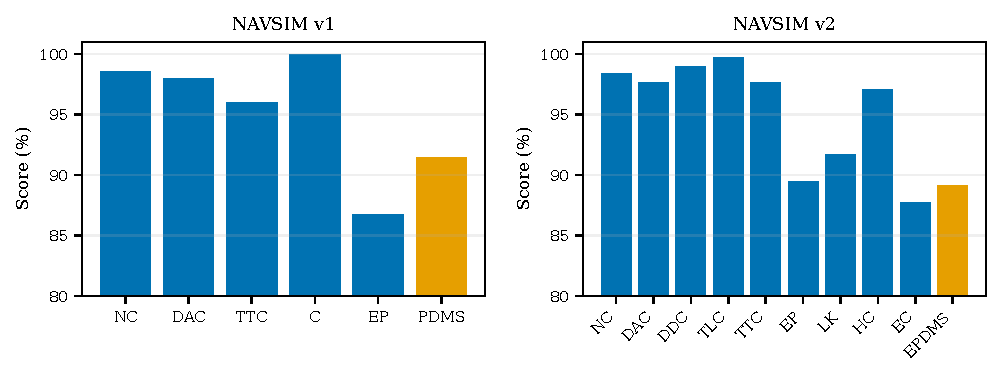
\includegraphics[width=0.76\textwidth]{figures/generated/ampt_metric_profiles.pdf}
  \caption{Scene-level reproduced AMPT component profiles on NAVSIM v1 and
  v2.  All metrics are percentages and higher is better; aggregate PDMS/EPDMS
  is shown in orange.  The profiles use 12,138 and 12,146 scored scenes,
  respectively, from one inference realization.}
  \label{fig:metric-profiles}
\end{figure*}

\paragraph{Single-trajectory inference.}
For each scene and inference seed, the model receives one observation, runs one
five-step denoising chain, and submits its single final $8\times3$ trajectory.
There is no test-time group sampling, evaluator call, candidate scoring,
reference lookup, model ensemble, or reranking.  The v1 submission provenance
independently records candidate count one, so this is a scene-level reproduced
property rather than only a methodological statement.

\paragraph{Runs and uncertainty.}
The archived v1/v2 headline exports each establish a scene-level mean for one
policy realization; they do not establish across-seed variance.  We therefore
do not attach a fabricated standard deviation to the 0.1--0.3 point increments
in the paper.  For the proposed rerun, each of seeds
20260726/20260727/20260728 produces a
complete scene export.  We first compute the mean for each run and report the
mean $\pm$ standard deviation across the three runs.  Method differences use
10,000 paired bootstrap resamples of shared scenes (resampling seeds and then
scenes within seed when multiple seeds are present), with a fixed analysis seed
of 2027 and a two-sided 95\% interval.  Recovery proportions use Wilson 95\%
intervals.  Scene bootstrap intervals from one model run describe variation
over the evaluated scenes and are explicitly not interpreted as training-seed
stability.

\paragraph{Model selection disclosure.}
The archived final v1 provenance states that \texttt{navtest} participated in
checkpoint selection.  We therefore describe the headline table as a
paper-reported benchmark comparison, not as a clean held-out model-selection
study.  The proposed rerun selects checkpoints only on the training/validation
partition, seals a checkpoint hash before \texttt{navtest}, and evaluates each
sealed hash once per inference seed.  This disclosure does not change a main
paper number; it narrows the fairness claim to what the available provenance
supports.

\subsection{The Fixed 658-Scene Recovery Protocol}
\label{sec:hard658-protocol}

The hard population is fixed before comparing optimization methods.  A scene
enters the set when the ReCogDrive IL policy receives PDMS zero in all five
sampling attempts because of collision, drivable-area violation, or both.
The resulting intersection contains 658 scene IDs.  A method \emph{recovers} a
scene when its single submitted trajectory has PDMS strictly greater than
zero under the same evaluator; the threshold is not retuned per method.

For consistency with the main paper, every supplementary hard-set analysis
uses the same archived scalar-GRPO versus historical Core-Pareto recovery pair that produced
367 and 440 positive-score scenes.  It does not substitute a later
full-benchmark checkpoint.  On the 658 fixed scenes, scalar GRPO has 367
positive and 291 zero-score outcomes, whereas the manuscript recovery
checkpoint has 440 positive and 218 zero-score outcomes.  Their paired
transition counts are 347 retained successes, 20 new failures, 93 repaired
failures, and 198 persistent failures.  Hence the net recovery is
$93-20=73$ scenes, exactly the change $440-367$, rather than a gain obtained by
hiding newly failed scenes.  The corresponding recovery rates are 55.8\%
(Wilson 95\% CI 52.0--59.5; $n=658$) and 66.9\% (63.2--70.4; $n=658$).  A
10,000-sample paired scene bootstrap gives an absolute difference of 11.1
percentage points with a 95\% interval of 8.1--14.3 points.
These intervals describe one archived checkpoint pair; no training-seed
identifier was retained for this hard-set export.

The fixed-set construction contains 480 DAC-only, 165 collision-only, and 13
joint collision-and-DAC cases according to the archived cause manifest.  The
same IDs and failure labels are used in all hard-set transition and case-table
analyses.  In particular, ``440 recovered'' means 440 positive outcomes on the
fixed original population; the transition table is required whenever the
claim is interpreted as a policy-to-policy improvement.

\subsection{Baseline and Controlled-Comparison Protocol}
\label{sec:baseline-protocol}

\input{tables/generated/baseline_protocol.tex}

AMPT's v1 and v2 rows are locally reproduced from scene-level outputs.  Other
headline baseline rows are values reported in the main paper and their cited
sources; no local checkpoint, common prediction export, or common seed manifest
was found for them.  They are consequently labeled \emph{reported}, not
\emph{reproduced}.  The table records backbone, sensor interface, training
data, number of inference candidates, and use of a test-time scorer whenever
the cited evidence establishes those fields.  An unavailable field is marked
``not established by the audited source'' rather than filled by analogy with
AMPT.

For the GT/Score/Pareto/PC-MTS comparison, the paper reports a shared
initialization, diffusion SFT loss, optimizer, epoch budget, scalar-GRPO
configuration, and evaluation protocol.  The controlled reproduction
additionally seals the candidate-source manifest, fixes the proposed non-GT
sampling probability, matches the accepted candidate count, draws one target
per scene-update, and uses the same three proposed training seeds.  For Scalar GRPO versus FF-PGRPO, all rollout
chains are generated from the same initialization and sampled with the same
seed before the credit function is changed.  For No APR versus Full APR, total
optimizer steps are matched by continuing the no-APR policy with retention
targets.  These are proposed control procedures until their launch manifests
and outputs exist; the main-paper point estimates remain labeled
paper-reported.

\subsection{Reproduction and Integrity Checks}
\label{sec:reproduction-checks}

The canonical dataset stores normalized scores, benchmark and split, method,
stage, variant, round, scene ID, seed when recorded, feasibility/failure
transitions, teacher status, and its source-file/key provenance.  Validation
checks expected scene counts, duplicate scene-method records, score ranges,
the benchmark aggregate formulas, paired scene sets, and failure-state logic.
Final tables and figures are generated from that dataset; a validation failure
stops manuscript generation.  The build manifest records the command, analysis
seed, package versions, Git revision, and SHA-256 hashes of inputs and outputs.
All raw result directories are read-only, and all derived files remain under
the supplementary directory.

  \section{PC-MTS Analyses: Supervision--Optimization Alignment}
\label{sec:pcmts-analysis}

This section is needed because the quality of a supervision target and its
value for subsequent policy optimization are different quantities.  PC-MTS is
designed for the latter: it keeps a target only when its score, component-wise
trade-off, local feasibility, and proximity to the frozen learner's rollout
support are jointly acceptable.  We first examine the observed
imitation-to-optimization reversal, and then specify the controls required to
separate policy compatibility from candidate count and training budget.

\subsection{The observed supervision--optimization reversal}
\label{sec:pcmts-mismatch}

Table~\ref{tab:supervision_mismatch} restates the reported comparison from the
main paper and makes the change induced by the common scalar-GRPO stage
explicit.  Score and Pareto selection produce the two strongest imitation
checkpoints (87.2 and 87.5 PDMS), yet both deteriorate under the subsequent
optimizer.  In contrast, PC-MTS deliberately gives up 0.3--0.6 imitation
points relative to those selectors and improves by 4.2 points after the same
optimization stage.  GT supervision also improves, but finishes 0.8 points
below PC-MTS.  Thus, ranking target sets by imitation PDMS would select Pareto,
whereas ranking them by optimized PDMS selects PC-MTS.  This reversal is the
direct evidence for the mismatch claimed in the paper.

\input{tables/generated/supervision_mismatch.tex}

\begin{figure}[t]
  \centering
  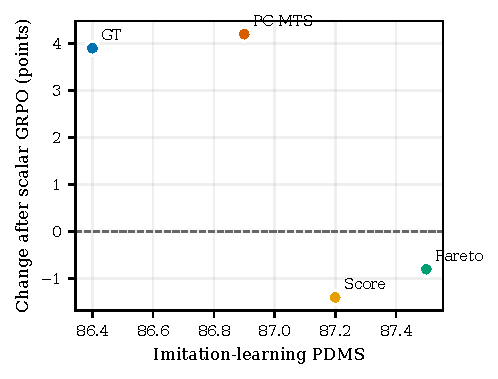
\includegraphics[width=\linewidth]{figures/generated/supervision_mismatch.pdf}
  \caption{Paper-reported imitation PDMS versus the change after the common
  scalar-GRPO stage on NAVSIM v1.  A high imitation score alone does not
  predict optimization value: Score and Pareto regress, whereas PC-MTS gains
  4.2 points.  Each marker is one reported point estimate; the paper does not
  state run/seed aggregation and no synthetic error bars are shown.}
  \label{fig:supervision-mismatch}
\end{figure}

The comparison should be interpreted at the level supported by the evidence.
It demonstrates that a higher-scoring imitation checkpoint need not be a
better starting distribution for GRPO, and that the PC-MTS set is compatible
with a large positive update in this run.  The archived paper table does not
contain scene-level outputs, acceptance counts, or multiple seeds for these
four cells.  Consequently, it does not by itself establish that the reversal
is invariant to seed, nor does it isolate candidate count from the four
filtering decisions.  We therefore do not attach synthetic error bars or
policy-distance values to these points.

\subsection{Candidate-count-matched reconstruction protocol}
\label{sec:pcmts-matched-protocol}

The released reproduction configuration turns the missing causal controls
into a predeclared, low-ambiguity experiment.  All four variants start from the
same GT-only checkpoint, use the same candidate sources, contribute exactly
one target per scene and update, train imitation learning for 200 epochs, and
then run scalar GRPO with 16 rollouts per scene for 10 epochs.  Within each
navigation-command/source stratum, accepted candidates are deterministically
subsampled to the smallest retained count across variants.  The non-GT
sampling probability is held fixed, so a method cannot receive more gradient
updates merely because it retains more candidates.  Empty strata fall back to
the logged trajectory.  In addition to final PDMS, a 300-update diagnostic
records the early GRPO gain before long-horizon training effects can dominate.

For a fully specified reconstruction when the original resolved PC-MTS
manifest is unavailable, the release marks the following as \emph{proposed
reproduction settings}, not measured settings of the reported run: a rollout
bank of 16, $K=3$ neighbors, a command-conditional 0.95 calibration quantile,
and eight temporally correlated local perturbations.  The rollout bank and
calibration queries are disjoint by construction.  Three predeclared training
seeds (20260726, 20260727, and 20260728) are used for the reconstruction, while
bootstrap seed 2027 is reserved for analysis and is never treated as an additional
training run.  These choices fill the executable configuration without
retroactively attributing unrecorded hyperparameters to the main-paper result.

For each run, the pipeline records retained candidates, acceptance rate,
candidate-source composition, feasible rollout rate, feasible high-quality
rate, all-infeasible-group rate, zero-score rate, the 10th percentile,
CVaR-10, 300-update gain, and final scalar-GRPO PDMS.  Method differences are
computed on identical scenes with a 10,000-resample paired bootstrap; means
and standard deviations are reported across the three training seeds.

\subsection{Filter attribution and sensitivity}
\label{sec:pcmts-components}

The component experiment is cumulative: (i) aggregate Score only, (ii) Score
plus the component-wise Pareto gate, (iii) the preceding gates plus calibrated
policy compatibility, and (iv) the full selector with local-feasibility
testing.  Counts are matched after each gate, rather than relaxing a stricter
gate to reach a target count.  This distinction matters: a matched count must
not reintroduce candidates that failed the mechanism being tested.  The
decisive diagnostic is not imitation PDMS alone, but whether adding a gate
raises feasible rollout density and converts the fixed-budget GRPO change from
negative to positive.

The companion sensitivity protocol varies one factor at a time: rollout-bank
size in $\{8,16,32\}$, $K$ in $\{1,3,5\}$, calibration quantile in
$\{0.90,0.95,0.975\}$, and perturbation count in $\{4,8,16\}$.  Compatibility
alternatives are compared at the same acceptance rate: candidate-to-GT
ADE/FDE, distance to the deterministic policy output, minimum rollout-bank
distance, average $K$-nearest distance, and command-calibrated $K$-nearest
distance.  These are evidence-bounded planned analyses: the release contains
their configurations and logging schema, but no unexecuted outcome is used to
support the paper's reported 91.1 PDMS.

Taken together, the existing reversal and the matched protocol close two
different parts of the argument.  The former establishes that isolated target
quality can disagree with downstream optimization value; the latter defines
the experiment needed to attribute that disagreement specifically to policy
compatibility rather than supervision quantity.

  \section{FF-PGRPO Analyses: Feasibility Before Positive Credit}
\label{sec:ffpgrpo-analysis}

Aggregate reward can hide an unsafe trade: progress or comfort may increase
enough to give positive standardized advantage even when collision avoidance,
drivable-area compliance, or a protected reference metric regresses.  The
purpose of FF-PGRPO is therefore not merely to reshape the scalar score, but to
change which rollouts are eligible for positive credit.

\subsection{What the stage ablation establishes}
\label{sec:ffpgrpo-stage-ablation}

On NAVSIM v1, the no-stage baseline in the main ablation has 86.5 PDMS, 98.1
NC, 94.7 DAC, 94.2 TTC, and 80.9 EP.  Applying FF-PGRPO without PC-MTS reaches
91.0 PDMS, with 98.4 NC, 98.0 DAC, 95.8 TTC, and 85.93 EP.  With PC-MTS as the
initialization, FF-PGRPO reaches 91.1 PDMS, 98.5 NC, 98.0 DAC, 96.0 TTC, and
86.0 EP before APR.  The improvement is therefore not produced by sacrificing
the displayed hard-safety components for progress: DAC improves by 3.3 points
and TTC by 1.6 points in the FF-PGRPO-only row, while EP increases by 5.03
points.  These are paper-reported point estimates whose run/seed aggregation
is not stated, so the small 0.1-point
difference between the two FF-PGRPO rows is not presented as a stable gain.

\input{tables/generated/stage_ablation.tex}

This result is consistent with the proposed ordering---recover feasibility,
then optimize continuous quality---but an aggregate stage ablation cannot
directly reveal the sign of individual rollout credits.  The fixed hard-scene
transition in Section~\ref{sec:hard658} provides scene-level evidence, and the
instrumentation below defines the rollout-level test.

\subsection{Credit diagnostics}
\label{sec:ffpgrpo-credit-diagnostics}

For rollout $i$, let $A_i>0$ denote positive assigned advantage and let
$V_i=1$ denote a violation of any hard-feasibility, protected-reference, or
admissible-Pareto condition.  We report
\begin{equation}
  \mathrm{PCVR} =
  \frac{\sum_i \mathbb{1}[A_i>0]V_i}
       {\sum_i \mathbb{1}[A_i>0]},
  \label{eq:positive-credit-violation}
\end{equation}
and separately count reference-regressing and Pareto-dominated positive
credits.  A denominator of zero is reported as ``no positive credits,'' not as
zero violation.  FF-PGRPO's implementation makes a violating rollout
ineligible for positive credit and exposes assertions for this contract.  The
archived training run, however, does not contain the per-rollout trace needed
to quote an observed PCVR; we do not convert a code invariant into a fabricated
measured rate.

The stepwise mechanism ablation adds: (i) the hard feasibility gate, (ii) the
coherent-reference guard, (iii) the Pareto positive-credit gate, and (iv) the
all-infeasible recovery rule.  Every variant logs group state
(all-feasible/mixed/all-infeasible), feasibility rate, positive and negative
advantage means, PCVR, reference-regressing positive-credit rate,
dominated-positive-credit rate, zero-to-feasible repair, positive-to-zero
regression, and updates until the first feasible rollout.  The coherent
reference is always one executable trajectory.  The historical
component-wise envelope remains only as an ablation because combining the best
value of each metric from different trajectories may describe no realizable
plan and can make every sampled rollout appear to regress.

The low-cost diagnostic run uses the paper's group size of 16 and stops at 300
updates; the final run uses the reported 10 epochs.  All variants share the
same sampled rollout tensors when credit is recomputed offline, which makes
the initial credit-assignment comparison independent of policy drift.  New
training is required only for the subsequent learning curves and remains
disabled unless explicitly enabled.

\subsection{Hard-scene evidence for feasibility-first recovery}
\label{sec:ffpgrpo-hard-evidence}

The manuscript recovery checkpoint is evaluated on the same 658-scene set as
scalar GRPO.  Scalar GRPO produces a positive score in 367 scenes (55.8\%,
95\% Wilson CI 52.0--59.5\%), whereas the AMPT recovery checkpoint is positive
in 440 scenes (66.9\%, CI 63.2--70.4\%).  The comparison uses a single
trajectory per scene and neither method uses test-time sampling, scoring, or
reranking.  Crucially, the paired transition is not merely a difference of
gross counts: 93 scalar-GRPO zeros become positive, 20 scalar-GRPO positives
become zero, 347 successes are retained, and 198 failures persist.  Net
recovery is therefore $93-20=73$ scenes, or 11.1 percentage points.  A
10,000-resample scene-paired bootstrap (analysis seed 2027) gives a 95\% CI of
8.1--14.3 percentage points for this paired change.  This interval quantifies
scene variation for this fixed checkpoint pair; it does not replace missing
multi-seed training uncertainty.

The subset mean PDMS increases from 0.5101 to 0.6145.  The corresponding
component means change from 0.8381 to 0.8815 for NC, 0.7052 to 0.7781 for DAC,
0.7705 to 0.8161 for TTC, and 0.4956 to 0.5932 for EP; comfort increases from
0.9985 to 1.0000, while DDC changes from 0.9567 to 0.9521.  This last decrease
is why protected metrics must be reported next to aggregate recovery rather
than summarized as universal component-wise improvement.  The complete
transition and failure-type decomposition are given in
Section~\ref{sec:hard658}.

The aggregate ablation, paired hard-scene transition, and positive-credit
instrumentation serve complementary roles.  The first shows the overall stage
gain, the second verifies that recovery is net positive rather than purchased
entirely with new failures, and the third is the predeclared test of the
claimed credit-assignment mechanism.

  \section{APR Analyses: Dynamic, Policy-Relative Teachers}
\label{sec:apr-analysis}

APR addresses a moving-target problem.  A trajectory that is a useful local
teacher for the current policy can become redundant after refinement, while a
previously distant candidate can enter the policy's compatible neighborhood.
The relevant question is therefore not whether additional optimization steps
help, but whether rebuilding and re-auditing the teacher set provides useful
targets while retaining already safe behavior.

\subsection{Round-wise behavior and protected components}
\label{sec:apr-rounds}

The main paper reports a monotonic sequence of 91.10, 91.21, 91.37, and 91.45
PDMS from Round 0 through Round 3, corresponding to gains of $+0.11$, $+0.16$,
and $+0.08$.  In the stage ablation, adding APR to the PC-MTS+FF-PGRPO policy
raises PDMS from 91.1 to 91.4 and EP from 86.0 to 86.7, while the displayed NC,
DAC, TTC, and comfort values remain 98.5, 98.0, 96.0, and 100, respectively.
This pattern is aligned with APR's design: local teacher updates increase
progress without visible regression in the protected components at the
reported precision.

Each round value is a reported checkpoint summary; its run/seed aggregation is
not stated.  No across-seed
standard deviation is available, and the 0.08--0.16 point increments are not
claimed to be independently significant.  Moreover, the archived experiment
history contains accepted and rejected branches rather than a single complete
three-round hash chain; the four values above are therefore treated as the
paper's round-level summary, not as permission to infer missing intermediate
measurements.

\input{tables/generated/apr_rounds.tex}

\begin{figure}[t]
  \centering
  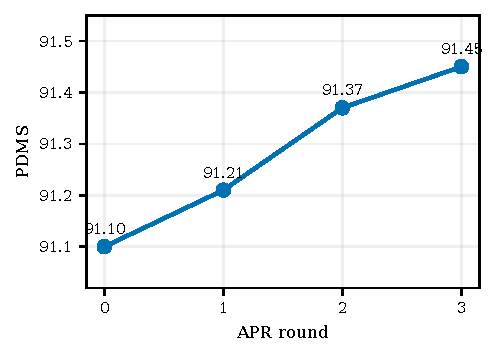
\includegraphics[width=\linewidth]{figures/generated/apr_rounds.pdf}
  \caption{Paper-reported NAVSIM v1 progression across APR rounds.  The final
  point is reproduced at scene level, but the small round increments are from
  one reported sequence and carry no across-seed error bar.}
  \label{fig:apr-rounds}
\end{figure}

\subsection{Teacher audit and post-interpolation evaluation}
\label{sec:apr-teacher-audit}

One traceable APR teacher-construction pass starts from 39,261 strict external
trajectories: 25,402 (64.7\%) from one driving-policy source and 13,859
(35.3\%) from a second source.  After interpolation with coefficient 0.25 and
exact re-evaluation, 28,910 targets remain, an acceptance rate of 73.6\%; the
remaining 10,351 are rejected.  These counts are from one audited navtrain
construction pass and are not presented as the source proportions of every
APR round.  They nevertheless establish an important operational fact:
interpolation is followed by evaluator-based admission, and the check is
non-vacuous---more than one quarter of the pre-audit union does not enter the
distillation set.

\input{tables/generated/apr_teacher_pool_audited.tex}

Teacher status is defined relative to the current policy.  A candidate is
\emph{accepted} when its evaluated local target is feasible, exceeds the
current single prediction by the required margin, preserves protected
metrics, and stays inside the current rollout neighborhood.  An accepted
teacher becomes \emph{expired} if it fails those tests after the policy is
updated.  A previously rejected candidate is \emph{newly activated} if it
passes after the rollout bank and current prediction are regenerated.  These
definitions prevent lifecycle counts from being conflated with raw pool size.

The interpolation search is descending: larger moves are evaluated first and
the first admissible move is retained.  Every accepted target stores the
teacher, current prediction, interpolation coefficient, post-interpolation
score, protected-metric deltas, compatibility distance, and evaluator hash.
No-interpolation and no-post-evaluation controls remove different safeguards:
the former jumps directly to the teacher, whereas the latter retains a local
trajectory without verifying that interpolation preserved feasibility.

\subsection{Step-matched controls}
\label{sec:apr-controls}

The release defines eight variants from the same Round-0 checkpoint and
matches the total number of optimizer updates: extra training on the existing
mixture, one-shot distillation, repeated use of a fixed teacher set, dynamic
teachers, dynamic teachers without interpolation, without post-interpolation
re-evaluation, without policy retention, and full APR.  The dynamic-teacher
and full-APR variants rebuild predictions, rollout banks, and teacher audits at
the same three round boundaries reported in the paper.  The fixed-teacher
variant repeats the Round-1 set without re-ranking it; the extra-training
control receives the same update count but no new teacher target.  This design
separates four possible explanations: more updates, teacher supervision in
general, teacher-set rebuilding, and the interpolation/retention safeguards.

For every round, the required report contains PDMS and all components,
regressed scenes, new failures, accepted/expired/newly activated teachers,
mean and median verified teacher advantage, interpolation-coefficient
distribution, and scene coverage.  A checkpoint is promoted only if its
single-trajectory aggregate score improves and protected metrics pass the
same non-regression audit; otherwise the previous checkpoint remains the
dynamic anchor.  Training ends after three promoted rounds or when no audited
local target remains.  These controls are configured but not represented as
measured results in this supplement, because running them would require new
training.

Optional task-vector consolidation is kept separate from teacher discovery.
The implementation can mask low-salience coordinates, require directional
agreement, bound each branch norm and the total displacement from the current
anchor, and then evaluate the merged checkpoint.  The best-branch, simple
average, task-arithmetic, and TIES-style controls are required before assigning
an independent gain to merging~\cite{taskarithmetic2023,ties2023}.  In the
absence of a stable, step-matched gain, merging should be read as a conservative
checkpoint-consolidation detail, not as the source of APR's teacher lifecycle.

The present evidence therefore supports two bounded statements: the reported
APR rounds are monotonic and preserve the displayed safety/compliance metrics,
and an audited construction pass materially filters proposed local targets
after re-evaluation.  The step-matched variants above are the necessary test
for the stronger causal claim that dynamic rebuilding, rather than additional
training alone, explains the full increment.

\input{tables/generated/apr_fixed_teacher_diagnostic.tex}

  \section{Failure Recovery and Qualitative Diagnostics}
\label{sec:failure-qualitative}

Qualitative evidence is most useful when organized by a mechanism and tied to
scene-level metrics.  We therefore analyze the fixed hard set first, then give
traceable examples of recovered, persistent, and newly introduced failures.
All quantitative hard-set results and the mechanism-organized case table use
the same historical checkpoint pair as the main paper's 367-versus-440
recovery claim.  The final full-benchmark visualization is separately labeled
and is not used in the 658-scene recovery analysis.

\subsection{Construction of the fixed 658-scene set}
\label{sec:hard658}

The set contains 658 NAVSIM v1 scenes for which the initial ReCogDrive policy
obtained exactly zero PDMS in all five construction samples because of an
at-fault collision (NC), drivable-area violation (DAC), or both.  The set is
fixed before comparing the scalar-GRPO and AMPT recovery checkpoints.  Under
single-trajectory evaluation, scalar GRPO is positive on 367 and zero on 291
scenes; the AMPT recovery checkpoint is positive on 440 and zero on 218.

The paired $2\times2$ transition is
\begin{equation}
\begin{array}{c|cc|c}
 & \multicolumn{2}{c|}{\text{AMPT recovery checkpoint}} & \\
\text{scalar GRPO} & \text{zero} & \text{positive} & \text{row total} \\
\hline
\text{zero}     & 198 & 93  & 291 \\
\text{positive} & 20  & 347 & 367 \\
\hline
\text{column total} & 218 & 440 & 658
\end{array}.
\label{eq:hard658-transition}
\end{equation}
Hence 93 failures are repaired, 347 successes are retained, 198 failures
persist, and 20 new failures appear.  The net change is $93-20=73$, exactly the
difference between the gross positive counts $440-367$.  This distinction is
important: 440/658 is the gross recovery rate relative to the policy used to
construct the hard set, whereas 93 and 20 describe the paired transition from
scalar GRPO to the AMPT recovery checkpoint.  The resulting 11.1-percentage-
point paired improvement has a scene-bootstrap 95\% CI of 8.1--14.3 points
(10,000 resamples, seed 2027).  It is a net improvement rather than an exchange
of an equal number of old and new failures.

\input{tables/generated/failure_recovery.tex}
\input{tables/generated/failure_net_gain.tex}

\begin{figure}[t]
  \centering
  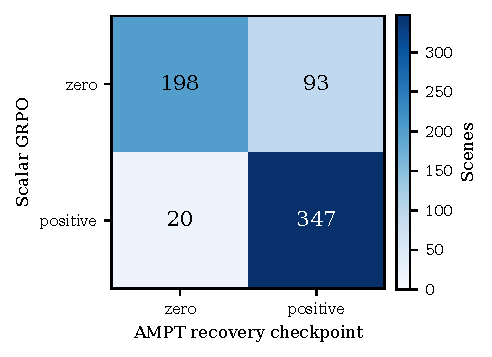
\includegraphics[width=\linewidth]{figures/generated/failure_transition.pdf}
  \caption{Scalar-GRPO to AMPT transition on the fixed 658-scene set.  The
  off-diagonal cells expose both 93 repairs and 20 regressions, rather than
  reporting gross recovery alone.}
  \label{fig:failure-transition}
\end{figure}

The original hard-set taxonomy contains 480 DAC-only scenes, 165 collision-
only scenes, 13 scenes failing both, and no residual ``other'' category.  The
paired repairs/new failures are 59/14 for DAC-only, 32/6 for collision-only,
and 2/0 for the joint category, giving net changes of 45, 26, and 2 scenes.
The gains are therefore not concentrated in only one failure type, although
the small joint category is descriptive rather than statistically decisive.

\input{tables/generated/failure_cause_breakdown.tex}

\begin{figure}[t]
  \centering
  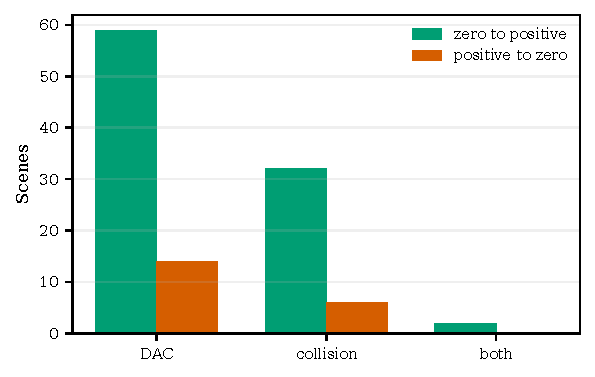
\includegraphics[width=\linewidth]{figures/generated/failure_cause_recovery.pdf}
  \caption{Repairs and regressions by the fixed hard-set cause taxonomy.  The
  net changes are 45 DAC, 26 collision, and 2 joint cases, totaling 73.}
  \label{fig:failure-causes}
\end{figure}

\subsection{Traceable scene cases}
\label{sec:traceable-cases}

Table~\ref{tab:hard658-cases} selects cases by transition type, not by visual
appeal.  Navigation commands come from the corresponding NAVSIM scene
metadata; scores and components come from the fixed paired evaluation.  The
table uses full scene identifiers so every row can be regenerated.  Component
pairs are scalar-GRPO $\rightarrow$ AMPT-recovery values.

\input{tables/generated/failure_cases.tex}

The first two cases are consistent with feasibility-oriented recovery: a hard
component changes from zero to one and positive PDMS returns.  Scene-level
before/after metrics do not identify the temporal order of training updates.
The third shows why ``recovered'' does not mean component-wise perfect.  The
fourth remains a DAC/progress failure under both audited checkpoints; without a
candidate/rollout manifest, the metrics do not identify whether pool coverage,
policy support, or optimization is responsible.  The fifth prevents
survivorship bias in the qualitative analysis and
motivates APR retention; it is one of the 20 positive-to-zero transitions
already charged against net recovery.

\subsection{Mechanism-centered visualization protocol}
\label{sec:qualitative-protocol}

The supplied renderer groups panels by decision rather than by scene
similarity.  A PC-MTS panel overlays an accepted candidate, a rejected distant
candidate, the logged trajectory, and the frozen-policy rollout neighborhood.
An FF-PGRPO mixed-group panel distinguishes unsafe, feasible-but-dominated,
and admissible Pareto-positive rollouts and prints their assigned advantages;
an all-infeasible panel shows the coherent recovery reference.  An APR panel
shows the current prediction, raw teacher, evaluated interpolant, and the
accepted/expired/newly-activated lifecycle state.  Every rendered panel reads
the scene id, command, component scores, and method name from its manifest and
uses a common legend: blue for the current prediction, green for an accepted
or positively credited trajectory, orange for a dominated/expired trajectory,
red for an unsafe trajectory, and black dashed for the coherent reference.

This protocol is also a safeguard against overinterpretation.  A camera/BEV
image is emitted only when the frame, command, all trajectories, and evaluator
record share the same scene identifier.  The metric-only cases in
Table~\ref{tab:hard658-cases} remain quantitative case studies if those visual
assets are unavailable; no unrelated camera frame or hand-drawn trajectory is
substituted merely to complete a panel.

\begin{figure*}[t]
  \centering
  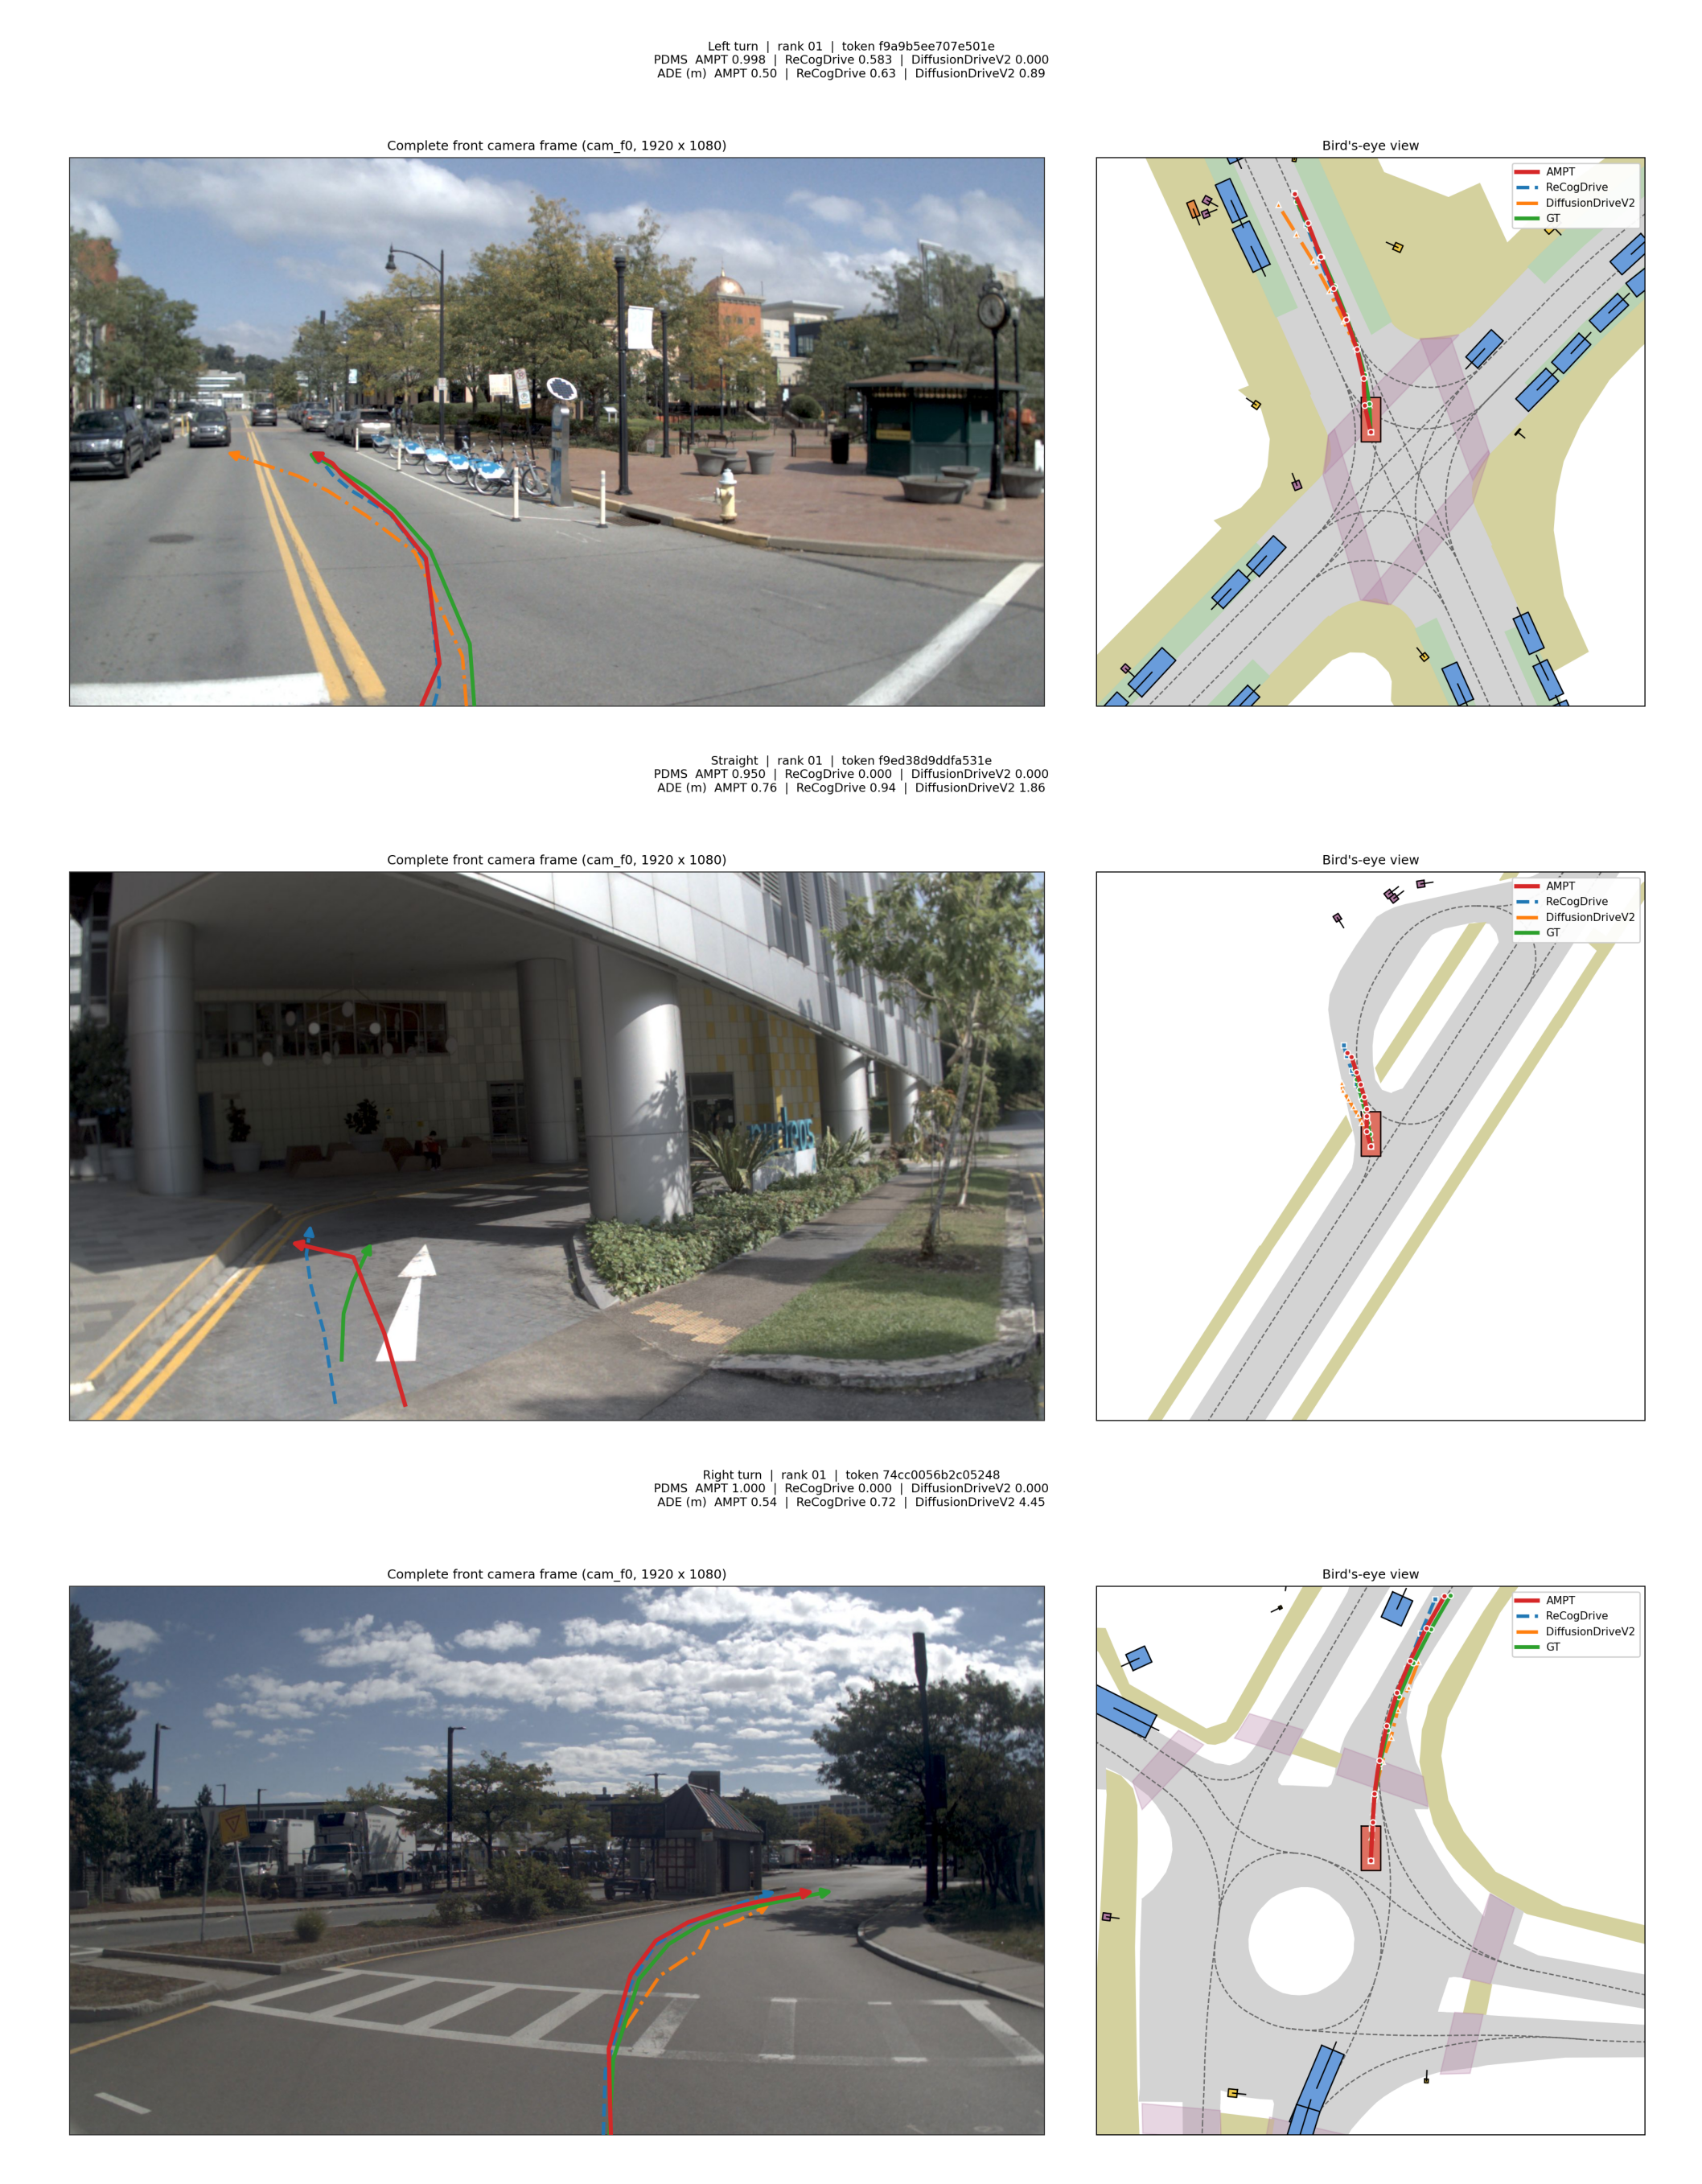
\includegraphics[width=0.92\textwidth]{figures/generated/qualitative_selected_cases.png}
  \caption{Three selected full-benchmark NAVSIM v1 cases (left, straight, and
  right commands) rendered from the separately audited final-AMPT manifest.
  Each row contains the complete front frame, bird's-eye view, scene ID,
  command, color legend, PDMS, and trajectory error.  These examples are not
  members of, and contribute no statistics to, the historical 658-scene
  recovery comparison; they illustrate final-policy behavior only.}
  \label{fig:qualitative-selected}
\end{figure*}

\clearpage

  \section{Additional Related Work, Fair Comparison, and Limitations}
\label{sec:related-limitations}

\subsection{Related perspectives}

\textbf{Support-aware policy improvement.}
Conservative offline policy-improvement methods limit updates in regions where
the behavior data provide weak support.  SPIBB constrains uncertain decisions
to the baseline policy~\cite{spibb2019}, while BEAR regularizes a learned policy
toward the behavior distribution~\cite{bear2019}.  PC-MTS shares the support
intuition but applies it before optimization: it filters trajectory-level
supervision using samples from the frozen learner, with command-conditional
calibration and a local feasibility test.  It is not a general monotonic-
improvement guarantee; its role is to avoid moving the imitation policy into a
region where downstream rollout optimization has poor local support.

\textbf{Multi-objective and Pareto optimization.}
Multi-objective reinforcement learning studies policies under vector-valued
returns and alternative preference models~\cite{roijers2013}.  AMPT does not
seek a global set of Pareto-optimal policies.  PC-MTS uses a scene-local Pareto
filter for supervision, and FF-PGRPO uses a hierarchy: hard feasibility and
coherent-reference guards are evaluated before a rollout can receive positive
Pareto credit.  This order is essential when an aggregate score can compensate
for a protected regression.

\textbf{Advantage-weighted behavior learning.}
Advantage-weighted regression turns estimated advantages into weights for
supervised policy updates~\cite{awr2021}.  APR is related at the loss level,
but its weights are attached only after a candidate is compared with the
current single-trajectory prediction, locally interpolated, and re-evaluated.
Teacher admission and policy retention are therefore as important as the
weighting function itself.

\textbf{Model merging.}
Task arithmetic combines model displacements relative to a shared
anchor~\cite{taskarithmetic2023}, and TIES resolves redundancy and sign
conflicts before merging~\cite{ties2023}.  AMPT may use an anchor-constrained
variant to consolidate APR branches, but merging is optional and is separated
from teacher selection.  Passing parameter-space norm and sign checks does not
imply behavioral safety; every merged checkpoint must still undergo the same
single-trajectory evaluator audit.

\subsection{Fair-comparison boundary}
\label{sec:fair-comparison}

AMPT uses one predicted trajectory at inference.  Policy rollout banks,
candidate pools, coherent references, group sampling, specialist policies, and
the offline evaluator are training-only; there is no test-time scorer,
best-of-$N$ selection, or candidate reranking.  This contract is present in the
paper and is independently supported by the v1 submission provenance.

The released v1 scene export contains 12,138 successfully scored scenes from
12,146 predictions; the eight unscored predictions are disclosed rather than
imputed.  The v2 export contains 12,146 successful scene scores.  Its EC
aggregation follows the official evaluator, although a direct EC value is
present for 10,040 rows.  Scene-bootstrap intervals resample these scored
scenes and are explicitly labeled as scene uncertainty; they are not a
substitute for independent training runs.

The baseline rows in the main tables are treated as \emph{reported} unless a
local scene export and matching protocol are available.  AMPT's v1/v2 rows are
reproduced from scene-level outputs, but protocol matching is not established
for every external baseline.  Moreover, the audited v1 provenance records use
of navtest for checkpoint selection.  We therefore avoid a strict held-out
state-of-the-art claim and report protocol fields---backbone, sensors, training
data, inference candidates, and test-time scoring---alongside each comparison.

The 658-scene result uses the recovery checkpoint and checkpoint pair specified
by the main-paper analysis.  It is a fixed-subset diagnostic, not a claim that
every later checkpoint must induce the same transitions.  Reporting the full
$2\times2$ matrix in Eq.~\ref{eq:hard658-transition} makes the gross and net
notions of recovery explicit.

\subsection{Limitations}
\label{sec:limitations}

\textbf{Finite support estimates.}
Compatibility is estimated from a finite rollout bank.  Sparse commands or
multi-modal scenes can make a genuinely useful target appear distant, and the
calibrated neighborhood is only as representative as the frozen policy
samples.  Increasing bank size improves coverage but raises offline inference
and storage cost.

\textbf{Evaluator bias and non-reactive evaluation.}
All three stages use an offline NAVSIM evaluator for filtering, credit, or
teacher validation.  Systematic evaluator errors can therefore be amplified
across stages.  NAVSIM's non-reactive agents also cannot reveal how other road
users would respond to the learned trajectory; feasibility under this scorer
is not a closed-loop safety guarantee.

\textbf{Candidate-pool ceiling.}
APR can select and localize only behaviors represented in its multi-source
pool.  If no source proposes a valid maneuver, rebuilding the pool changes no
target.  The persistent case in Table~\ref{tab:hard658-cases} establishes
persistence under two audited checkpoints, but cannot diagnose this pool
ceiling without a per-scene candidate manifest.

\textbf{Locality can reject long-horizon value.}
The policy-compatibility filter intentionally favors learnable local targets.
It may reject a distant behavior that is initially difficult to imitate but
would be valuable after a longer curriculum.  Policy-dependent teacher-value
and cross-policy selection experiments are therefore important follow-ups.

\textbf{Benchmark-specific hierarchy.}
The ordering of NC/DAC feasibility, DDC/TLC guards, progress floors, and
continuous Pareto objectives reflects NAVSIM metrics.  Transferring AMPT to a
new benchmark requires revalidating the hierarchy and calibration thresholds,
not merely renaming metric fields.

\textbf{No behavioral semantics for parameter merging.}
Task-vector masks, direction agreement, and norm constraints bound parameter
movement but do not provide a semantic or safety guarantee.  If its independent
gain is not stable across seeds and step-matched controls, merging should
remain an implementation detail.

\textbf{Statistical scope.}
The supervision comparison, stage ablation, and APR round table are available
as reported point estimates rather than three-seed aggregates.  Small APR
increments must not be described as stable until the configured multi-seed
controls are run.  The paired 658-scene interval establishes a robust scene-
level net transition for one checkpoint pair, but does not measure training-
seed variation.

These limitations narrow rather than alter the paper's central claim.  The
currently traceable evidence establishes the supervision--optimization
reversal, a large feasibility-oriented stage gain, monotonic reported APR
rounds with preserved displayed safety components, and positive net recovery
on a fixed hard set.  Candidate-count matching, rollout-level credit traces,
step-matched APR controls, and multi-seed reruns are the remaining experiments
needed for stronger causal and stability claims.

  \expandafter\endinput
\fi

\documentclass[10pt,twocolumn]{article}
\usepackage[letterpaper,margin=0.72in]{geometry}
\usepackage[T1]{fontenc}
\usepackage{lmodern}
\usepackage{microtype}
\usepackage{amsmath,amssymb}
\usepackage{booktabs}
\usepackage{graphicx}
\usepackage{xcolor}
\usepackage{url}
\usepackage[hidelinks]{hyperref}
\setlength{\columnsep}{0.22in}
\setlength{\textfloatsep}{7pt plus 2pt minus 2pt}
\setlength{\floatsep}{6pt plus 2pt minus 2pt}
\setlength{\intextsep}{6pt plus 2pt minus 2pt}

\newcommand{\method}{AMPT}
\newcommand{\pc}{PC-MTS}
\newcommand{\ff}{FF-PGRPO}
\newcommand{\apr}{APR}
\newcommand{\reported}{\textsuperscript{R}}
\newcommand{\reproduced}{\textsuperscript{S}}
\newcommand{\proposed}{\textsuperscript{P}}

\title{Supplementary Material for\\
\textit{Aligning Multi-Trajectory Supervision with Policy Optimization for VLA Driving}}
\author{Anonymous Submission}
\date{}

\begin{document}
\maketitle
\begin{abstract}
This supplement specifies the three stages of Aligned Multi-Trajectory Policy
Training (AMPT), records implementation and evaluation provenance, and expands
the supervision, credit-assignment, policy-refinement, and failure-recovery
analyses.  Superscripts R, S, and P denote paper-reported, scene-level
reproduced, and proposed-but-unrun reproduction settings, respectively.  This
distinction prevents a proposed control from being mistaken for an observed
result.  Unless stated otherwise, evaluation emits one trajectory and performs
neither test-time scoring nor candidate reranking.
\end{abstract}

\appendix
\section{Additional Method Details}
\label{sec:additional-method}

This appendix makes explicit the contracts that connect the three training
stages.  This is important because the central claim of AMPT is not that a
trajectory with a high offline score is automatically a useful target, but
that supervision, rollout credit, and policy-relative refinement must agree on
what the current policy can safely learn.  We use three provenance labels
throughout.  \emph{Paper-reported} denotes a value stated in the main paper,
\emph{scene-level reproduced} denotes a value recomputed from an archived
per-scene evaluator export, and \emph{proposed reproduction} denotes a fully
specified setting for rerunning an experiment whose resolved training manifest
was not retained.  The last category is a protocol, not an observed result.

\subsection{Policy-Compatible Multi-Trajectory Supervision}
\label{sec:pc-mts-details}

\paragraph{Candidate construction and source balancing.}
For a scene $s$, let $\tau_s^0$ be the logged trajectory and let
$\mathcal C_s=\cup_m\mathcal C_s^{(m)}$ be the union of candidates supplied by
the configured proposal generators.  PC-MTS is source agnostic: a source may
be another policy seed, a structured trajectory expander, or a specialist
planner, but source identity is retained in the manifest and geometric near-
duplicates are merged before scoring.  The logged target is immutable and
is never removed.  A final Stage-1 source-count manifest was not found.  To
make the controlled reconstruction executable without presenting invented
counts as measurements, our \emph{proposed reproduction} caps every non-GT
source at eight candidates per scene before filtering.  When comparing Score,
Pareto, and PC-MTS, we use the same source
cap and retain the same number of non-GT candidates by taking the best valid
items under the corresponding rule.  Thus a difference cannot be attributed
to exposing one variant to a larger target set.

\input{tables/generated/candidate_source_statistics.tex}

\paragraph{Quality, feasibility, and Pareto filtering.}
Every complete trajectory is scored by the same offline evaluator used for
training diagnostics.  We first require hard feasibility, then a sufficient
aggregate score, and only then form the scene-wise component Pareto front.  A
candidate $a$ dominates $b$ only if it is no worse on every active Pareto
objective and is strictly better on at least one.  This order matters: a high
progress value cannot compensate for collision or leaving the drivable area.
The paper does not archive the numerical Stage-1 aggregate cutoff.  In the
\emph{proposed reproduction}, a training-split quantile is selected once so
that comparison variants are matched to the minimum retained count, followed
by a source-balanced top-$k$ tie break.  The sealed cutoff is applied
identically to all splits and is never used to synthesize a reported score.

The benchmark-specific partition is summarized below.  On NAVSIM v1, NC and
DAC are hard gates; DDC is protected; and EP, TTC, and comfort are optimized
inside the admissible region.  On NAVSIM v2, NC, DAC, DDC, and TLC are the
multiplicative compliance gates.  The historical metric adapter uses EP, TTC,
and a composite $Q=(\mathrm{LK}+\mathrm{HC}+\mathrm{EC})/3$ as its three
continuous Pareto axes; the official EPDMS report still exposes LK, HC, and EC
separately.  For binary scorer outputs the \emph{proposed reproduction}
requires a value of one up to $10^{-6}$.  The archived safety contract uses
reference-relative tolerances of $0.01$ for DDC/comfort and $0.02$ for TTC/EP;
TLC remains a hard v2 gate.  These are historical implementation values, not a
claim about the unresolved configuration of the paper checkpoint.

\input{tables/generated/metric_partition.tex}

\paragraph{Policy compatibility.}
Let $\mathcal R_s=\{\rho_j\}_{j=1}^{M}$ be rollouts sampled from the frozen
GT-only policy under the same command as the candidate.  We standardize
waypoint displacement with per-timestep, command-conditioned robust scales
fitted on the calibration split, and write the resulting trajectory distance
as $d(\tau,\rho)$.  The archived implementation additionally exposes final
displacement, heading, and velocity diagnostics, but the proposed controlled
comparison changes only the normalized waypoint statistic.  The compatibility
statistic is
\begin{equation}
 d_{\mathrm{PC}}(\tau,\mathcal R_s)
 =\frac{1}{K}\sum_{\rho\in\operatorname{NN}_{K}(\tau;\mathcal R_s)}
 d(\tau,\rho).
\end{equation}
The threshold $q_c$ is the command-specific quantile of leave-one-out policy
rollout distances on calibration scenes.  The archived code proves
leave-one-out calibration within each policy cloud, but its retained manifest
does not prove driving-log-level independence.  The proposed reconstruction
therefore enforces log-disjoint calibration and query scenes.  The paper states the general
$K$-nearest statistic but does not report $M$, $K$, or $q_c$.  The archived
implementation realizes the valid $K=1$ special case.  Our \emph{proposed
reproduction} uses $M=16$, $K=3$, and $q_c$ at the 95th percentile, with
command groups merged into a global fallback only when a command group has
fewer than 16 calibration observations.  This choice is also the center point
of the supplied sensitivity grid, rather than a retrospectively selected
result.

\paragraph{Local feasibility tube.}
Compatibility to one rollout neighborhood does not by itself establish that a
target is robust to small prediction errors.  For every candidate that passes
the previous gates, PC-MTS adds correlated perturbations to $(x,y,\psi)$ and
the implied velocity sequence.  The perturbations are sampled from normalized
policy residuals, smoothed over time, and projected back to the command-consistent
trajectory representation before exact re-evaluation.  This changes whole
trajectory segments rather than independently jittering waypoints.  The
archived implementation supports 16 or 32 perturbations; the \emph{proposed
reproduction} uses eight lower-cost perturbations, preserves the empirical
temporal covariance of policy residuals, and accepts a candidate when at least
six of eight perturbations pass
the hard feasibility gates and the protected guards.  The P1 configuration
evaluates 4/8/16 perturbations and does not tune the threshold on the test
split.

\paragraph{Target sampling and fallback.}
After filtering, the training set for scene $s$ is
$\mathcal T_s=\{\tau_s^0\}\cup\mathcal A_s$, where $\mathcal A_s$ contains
accepted candidates.  A training update draws exactly one target for the
scene, so scenes with many proposals do not receive larger gradients.  The
\emph{proposed reproduction} draws the logged target with probability $0.5$
and otherwise samples uniformly from $\mathcal A_s$; if $\mathcal A_s$ is
empty, it deterministically uses $\tau_s^0$.  Candidate identity is sampled
before the diffusion timestep, so all noisy versions in that update correspond
to a single coherent target.  Fine-tuning uses the same denoising objective as
GT-only training and produces $\pi_{\mathrm{initial}}$.

\paragraph{Implementation correspondence.}
The source-balanced builder and immutable-GT path are implemented at
\path{41a8613:navsim/agents/recogdrive/curriculum/builder.py}
and \path{41a8613:navsim/agents/recogdrive/curriculum/proposals.py}.
Physical distance and calibrated reachability are at
\path{41a8613:navsim/agents/recogdrive/curriculum/reachability.py};
the feasibility and correlated-perturbation checks are at
\path{41a8613:navsim/agents/recogdrive/curriculum/safety.py} and
\path{41a8613:navsim/agents/recogdrive/curriculum/robustness.py}.
These are historical mechanism-level implementations; the audit does not claim
that this commit is a complete hash-identical release of the final checkpoint.

\subsection{Feasibility-First Pareto GRPO}
\label{sec:ff-pgrpo-details}

\paragraph{A coherent scene reference.}
FF-PGRPO compares a rollout with one executable reference trajectory, never
with an envelope assembled from different trajectories.  The ordered source
set is: the logged trajectory, a retained PC-MTS candidate, and the current
single-trajectory prediction.  The paper-level rule selects the highest-scoring
feasible row.  The audited historical selector makes this precise by ranking
validity, hard feasibility, reference guard, robustness, core eligibility,
PDMS, distance to the current prediction, and source priority lexicographically.
Thus no higher score can bypass an earlier safety/eligibility tier.  If none is feasible, the
logged trajectory is retained only as a weak recovery target when it passes
the evaluator's basic physical checks.  Otherwise no recovery target is used
and every sampled rollout receives non-positive credit.  A component-wise
envelope is invalid because its NC, progress, and TTC values may come from
mutually incompatible plans; positive credit relative to such a synthetic
point would have no executable safety witness.

\paragraph{Group states and admissibility.}
For each scene the paper reports a group of $G=16$ policy rollouts.  We assign
the group to one of three states.  An \emph{all-feasible} group contains only
rollouts that satisfy hard feasibility; its quality statistic normalizes the
continuous score components because the binary gates are constant.  A
\emph{mixed} group contains both feasible and infeasible rollouts; feasibility
is applied first and feasible trajectories must additionally pass the coherent
reference guards.  An \emph{all-infeasible} group contains no feasible
rollout; it is not allowed to create a positive advantage by merely ranking
unsafe samples against one another.

For NAVSIM v1, admissibility requires NC and DAC and protects DDC, TTC, and an
EP floor relative to the coherent reference.  NAVSIM v2 additionally treats
DDC and TLC as hard compliance checks.  The archived safety-contract defaults
use $\mathrm{DDC}(\tau)\geq\mathrm{DDC}(r)-0.01$,
$\mathrm{TTC}(\tau)\geq\mathrm{TTC}(r)-0.02$, and
$\mathrm{EP}(\tau)\geq\mathrm{EP}(r)-0.02$.  The joint EP--TTC guard prevents
the optimizer from receiving positive credit for increasing safety merely by
stopping, or for increasing progress by collapsing the collision margin.

\paragraph{Credit assignment.}
Within a group that contains a feasible rollout, let $\widehat A_i$ be a
quality-shaped, group-relative score and let $P_i$ indicate membership in the
admissible Pareto front.  FF-PGRPO assigns
\begin{equation}
 A_i=\begin{cases}
 \max(\widehat A_i,0),
   & \substack{\text{feasible, guard-passing,}\\\text{and Pareto-positive}},\\
 \min(\widehat A_i,0),
   & \substack{\text{feasible but not}\\\text{admissible Pareto}},\\
 -\lambda_{\mathrm{unsafe}}+\min(\widehat A_i,0),
   & \text{infeasible}.
 \end{cases}
\end{equation}
Thus aggregate quality controls magnitude, whereas feasibility, a coherent
reference, and non-domination control the sign.  For mixed groups the quality
term also includes the EP-floor and joint EP--TTC penalties.  The historical
implementation preserves signs with RMS scaling rather than mean centering and
uses an archived default clip of $[-3,3]$; the \emph{proposed reproduction}
uses the predeclared sensitivity setting $[-5,5]$.

For an all-infeasible group, violation severity is the normalized sum of hard
gate deficits and protected-metric deficits.  Credit is the non-positive
within-group rank of negative severity, shifted by the unsafe penalty.  The
group loss is downweighted to $0.25$; when a valid recovery reference exists,
a diffusion recovery term with coefficient $0.25$ is added.  The proposed
regularization uses KL weight $0.02$ and anneals the BC coefficient linearly
from $0.10$ to $0.05$ over the first five epochs.  These numerical values are
historical implementation defaults and proposed rerun values, not recovered
resolved parameters for the paper's final FF-PGRPO run.

\paragraph{Diffusion credit and inference.}
One trajectory-level advantage is broadcast to every transition in that
trajectory's denoising chain.  The audited planner uses a discounted
transition-wise mean, while the paper objective writes the chain likelihood in
accumulated form; the proposed reconstruction preserves the planner reduction
and logs it in the resolved manifest.  This avoids assigning mutually
inconsistent metric credit to intermediate noisy states that are not executable
plans.  At inference, AMPT runs one denoising chain and emits one trajectory.
Group sampling, the Pareto computation, the reference selector, the offline
evaluator, and candidate reranking are absent from test time.

\paragraph{Implementation correspondence.}
Group classification, Pareto gating, violation ranking, sign-preserving
normalization, and clipping are at
\path{41a8613:navsim/agents/recogdrive/stage3_ff_pareto.py}.
The coherent-row API is at
\path{41a8613:navsim/agents/recogdrive/stage3_reference_selector.py},
and positive-credit assertions are at
\path{41a8613:navsim/agents/recogdrive/stage3_positive_credit_contract.py}.
The archived tensor layout is anchor-local; the paper-level protocol is the
union of 16 scene rollouts.  Because a final resolved layout manifest was not
found, we do not infer the number of anchors from a class default.

\subsection{Adaptive Pareto-Guided Policy Refinement}
\label{sec:apr-details}

\paragraph{Dynamic multi-source pool.}
At APR round $r$, the current policy $\pi_r$ supplies one local prediction for
every scene.  Candidate teachers come from historical policy checkpoints,
independent GRPO seeds, structured trajectory expansion, and safety-,
progress-, and regularity-oriented specialists.  Source labels survive
deduplication so per-source acceptance can be audited, but final three-round
source proportions were not archived.  The audited initial construction keeps
its observed 25,402/13,859 source mixture.  The proposed source-ablation reports
each source separately instead of claiming an unrecorded balancing rule.

\paragraph{Teacher audit.}
For a policy prediction $p_s$ and candidate teacher $t$, APR first requires
feasibility and an aggregate margin $R(t)-R(p_s)\geq m_R$.  It then applies
absolute and reference-relative protected guards.  Behavioral distance,
curvature, and jerk rank otherwise admissible teachers; they are preferences,
not claimed historical hard thresholds.  In the audited APR branch,
$m_R=0$ with a strict positive comparison, DDC has absolute floor 0.99 and
maximum drop 0.01, TTC has absolute floor 0.95 and maximum drop 0.02, and the
jerk coefficient 0.005 is a soft training regularizer.  At the interpolation
audit, the proposed reconstruction additionally applies the command-conditioned
95th-percentile compatibility calibration from PC-MTS.

\paragraph{Local interpolation and exact re-evaluation.}
An accepted teacher is not copied directly.  APR evaluates
\begin{equation}
 \tau_{s,\alpha}=p_s+\alpha(t-p_s)
\end{equation}
for a descending list of interpolation coefficients.  The first (largest)
coefficient that remains feasible, improves the aggregate score, preserves
protected metrics, and passes the current compatibility test becomes the local
target.  Every interpolated trajectory is scored anew; endpoint scores are
never linearly interpolated.  One audited branch used $\alpha=0.25$.  The
\emph{proposed reproduction} fixes the descending list to
$[1.0,0.75,0.50,0.25]$, which includes that audited setting and tests the
teacher endpoint before progressively more conservative steps.  If all
coefficients fail, the teacher is
rejected for the current round rather than kept with a smaller unscored step.

\paragraph{Weighted distillation, retention, and lifecycle.}
For verified gain $\Delta_s=R(\tau_{s,\alpha})-R(p_s)>0$, the target weight is
\begin{equation}
 w_s=\min\{5,\exp(\Delta_s/0.05)\}.
\end{equation}
The temperature $0.05$ and clip 5 are present in an audited APR training
branch.  The same diffusion denoising loss is applied to weighted local
targets, while current predictions provide retention targets with audited
weight 1.0.  At most the top one positive-advantage target is used per scene; a
scene without a valid teacher contributes retention only.  After training, the
candidate checkpoint is promoted only if aggregate validation score increases
and none of the protected aggregate components regresses beyond the audit
tolerances.  The promoted checkpoint becomes the dynamic anchor, its
predictions and rollout bank are regenerated, and the complete teacher pool is
audited again.  A previously accepted teacher is defined as \emph{expired} when
it loses its margin or guard, while a previously rejected one is \emph{newly
activated} when it passes under the new policy.  Historical scripts rebuild
round files but do not persist these labels; the proposed pipeline obtains them
by joining teacher hashes across consecutive round manifests.  The paper reports three
rounds.  The proposed stop rule is the earlier of three promotions, an empty
teacher set, or no checkpoint passing the promotion rule; it does not turn a
small unverified score fluctuation into a promotion.

\paragraph{Optional branch consolidation.}
Safety, progress, and regularity branches may be consolidated after their
teacher updates.  This is an optional checkpoint operation, not a substitute
for teacher auditing.  The audited anchor-constrained variant keeps the top
20\% salient coordinates of each base-relative task vector, removes
coordinates with inconsistent directions, clips every branch displacement to
the norm of its accepted branch, and caps total displacement at $1.05$ times
the largest accepted branch displacement.  The anchor is the current promoted
policy and is therefore updated across rounds.  If no merge candidate passes
the same evaluation guard as an ordinary APR checkpoint, the best accepted
single branch is retained.

\paragraph{Implementation correspondence.}
Teacher audits are implemented at
\path{fb96a03:scripts/stage3/build_pdms_strict_teacher_buffer.py}
and \path{fb96a03:scripts/stage3/build_pdms_safety_repair_teacher_buffer.py}.
Interpolation and exact rescoring are at
\path{ab9124c:scripts/stage3/build_pdms_blended_teacher_reference.py},
with local safety-tube checks at
\path{ab9124c:scripts/stage3/filter_pdms_teacher_reference_by_safety_tube.py}.
Retention schedules are built by
\path{fb96a03:scripts/stage3/build_pdms_teacher_refinement_schedule.py},
and the optional merge is at
\path{64f5531:scripts/stage3/merge_conflict_free_anchored_task_vector.py}.
APR is an orchestrated sequence of these audited operations; the repository
does not contain a single monolithic \texttt{APR.run} entry point.

\section{Algorithms}
\label{sec:algorithms}

The three procedures below are separated deliberately.  PC-MTS constructs a
supervision distribution before policy optimization; FF-PGRPO assigns credit
inside one rollout group; and APR rebuilds policy-relative teachers between
training rounds.  Combining them into one loop would obscure both their
different inputs and the interfaces tested by the implementation.  A code
comment names the closest audited historical function; ``paper contract''
marks a step for which no end-to-end final-checkpoint call graph was retained.

\paragraph{Algorithm 1: Policy-Compatible Multi-Trajectory Supervision.}
\label{alg:pcmts}
\begin{quote}
\small
\textbf{Input:} logged scenes $\mathcal D=\{(o_s,\tau_s^0,c_s)\}$; candidate
sources $\{\mathcal C_s^{(m)}\}$; frozen GT policy $\pi_{\mathrm{GT}}$;
offline evaluator $E$; compatibility and robustness configuration $\xi$.

\textbf{Output:} accepted per-scene target sets $\{\mathcal T_s\}$ and the
initialized policy $\pi_{\mathrm{initial}}$.

\begin{enumerate}
  \item Load source manifests, preserve source identity, form
  $\mathcal C_s=\cup_m\mathcal C_s^{(m)}$, merge geometric near-duplicates,
  and mark
  $\tau_s^0$ immutable.  \emph{Implementation:}
  \path{41a8613:navsim/agents/recogdrive/curriculum/proposals.py:load_scene_proposals},
  \path{deduplicate_proposals}; immutable retention is enforced by
  \path{builder.py:finalize_scene_record}.

  \item Evaluate every complete candidate with $E$; reject candidates that
  fail hard feasibility, the aggregate-quality threshold, intent checks, or
  reference-relative protected guards.  \emph{Implementation:}
  \path{41a8613:navsim/agents/recogdrive/curriculum/builder.py:build_scene_intermediate},
  \path{safety.py:absolute_feasibility} and
  \path{relative_nonregression}.

  \item Compute the component-wise Pareto front among survivors and apply the
  fixed source/role quota.  Do not allow a continuous metric to restore a
  candidate removed by a hard gate.  \emph{Implementation:} component-wise
  Pareto filtering is the paper contract; the audited tree exposes the later
  role/quota step at
  \path{41a8613:navsim/agents/recogdrive/curriculum/quota_selector.py:role_aware_quota_select},
  but no separately named Pareto-front function.

  \item Sample the policy rollout cloud $\mathcal R_s$ from frozen
  $\pi_{\mathrm{GT}}$.  Fit robust distance scales and command-specific
  quantiles using leave-one-out rollout queries.  Enforce log-disjoint
  calibration/query scenes in the proposed rerun; the archived manifest proves
  leave-one-out only.  \emph{Implementation:}
  \path{41a8613:navsim/agents/recogdrive/curriculum/builder.py:_policy_cloud_for_scene},
  \path{reachability.py:fit_reachability_calibration}.

  \item For each Pareto survivor $\tau$, compute its calibrated nearest-policy
  distance $d_{\mathrm{PC}}(\tau,\mathcal R_s)$ and retain it only when the
  relevant command threshold is met.  The archived branch implements $K=1$;
  the proposed rerun sets $K$ through $\xi$.  \emph{Implementation:}
  \path{41a8613:navsim/agents/recogdrive/curriculum/reachability.py:physical_distance_components},
  \path{evaluate_reachability}.

  \item Draw temporally correlated residual trajectories around every
  compatibility-passing candidate, score each perturbation with $E$, and keep
  the center candidate only if the required fraction remains feasible and
  guard-passing.  \emph{Implementation:}
  \path{41a8613:navsim/agents/recogdrive/curriculum/robustness.py:CorrelatedErrorModel.sample_perturbations},
  \path{evaluate_robustness_tube}.

  \item Set $\mathcal T_s=\{\tau_s^0\}\cup\mathcal A_s$.  If no non-GT
  candidate survives, set $\mathcal T_s=\{\tau_s^0\}$; never borrow a target
  from another scene.  \emph{Implementation:}
  \path{41a8613:navsim/agents/recogdrive/curriculum/builder.py:finalize_scene_record}.

  \item At each visit to $s$, sample exactly one member of $\mathcal T_s$
  according to the fixed GT/candidate mixture and then sample one diffusion
  timestep.  \emph{Implementation:}
  \path{41a8613:navsim/agents/recogdrive/stage2_role_sampler.py},
  \path{stage2_bridge.py}.

  \item Fine-tune a copy of $\pi_{\mathrm{GT}}$ with the unchanged diffusion
  noise-prediction loss and return it as $\pi_{\mathrm{initial}}$.
  \emph{Implementation:}
  \path{41a8613:navsim/agents/recogdrive/first_drive_v7_planner.py}.
\end{enumerate}
\end{quote}

\paragraph{Algorithm 2: Feasibility-First Pareto GRPO Credit Assignment.}
\label{alg:ffpgrpo}
\begin{quote}
\small
\textbf{Input:} scene $o_s$; policy $\pi_\theta$; the paper's $G=16$ sampled
denoising chains and final trajectories $\{(z_i,\tau_i)\}_{i=1}^{G}$; logged,
retained, and current-policy reference candidates; evaluator $E$; credit
configuration $\zeta$.

\textbf{Output:} trajectory advantages $\{A_i\}$ and the regularized
FF-PGRPO loss.

\begin{enumerate}
  \item Convert exact evaluator outputs for every $\tau_i$ to hard-feasibility,
  continuous-quality, protected-guard, and violation-severity tensors.
  \emph{Implementation:}
  \path{41a8613:navsim/agents/recogdrive/stage3_metric_adapter.py}.

  \item Rank complete logged, retained, and current-policy rows
  lexicographically by validity, hard feasibility, reference guard,
  robustness, core eligibility, PDMS, distance, and fixed source priority;
  choose the first row $r_s$.  Never take a different trajectory for each
  reference component.  Record whether a safe recovery reference is
  available.  \emph{Implementation:}
  \path{41a8613:navsim/agents/recogdrive/stage3_reference_selector.py:CoherentReferenceSelector.select},
  \path{gather_reference_rows}.

  \item Classify the rollout group as \textsc{all-safe}, \textsc{mixed}, or
  \textsc{no-safe}.  For safe rollouts, evaluate coherent-reference guards and
  admissible Pareto membership.  The audited function consumes anchor-local
  $[B,K,R]$ tensors; the final $K\times R$ layout is unresolved, so the proposed
  rerun seals $K=8,R=2$ to preserve $G=16$.  \emph{Implementation:}
  \path{41a8613:navsim/agents/recogdrive/stage3_ff_pareto.py:classify_group_state},
  \path{anchor_local_pareto}.

  \item If the state is \textsc{all-safe}, form $\widehat A_i$ from only the
  continuous score terms.  If it is \textsc{mixed}, form $\widehat A_i$ from
  aggregate quality plus EP-floor and joint EP--TTC shaping.  Preserve the
  scene grouping during normalization.  \emph{Implementation:}
  \path{41a8613:navsim/agents/recogdrive/stage3_ff_pareto.py:FeasibilityFirstCreditAssigner.compute}.

  \item For an \textsc{all-safe} or \textsc{mixed} group, set positive credit
  only for safe, guard-passing, Pareto trajectories; clamp safe dominated or
  guard-failing trajectories to non-positive credit; and apply an additional
  unsafe penalty to infeasible trajectories.  \emph{Implementation:}
  \path{41a8613:navsim/agents/recogdrive/stage3_ff_pareto.py:FeasibilityFirstCreditAssigner.compute}.

  \item For a \textsc{no-safe} group, rank negative violation severity and
  assign only non-positive credit.  Downweight the group and, if $r_s$ is a
  valid recovery reference, add weak diffusion supervision toward $r_s$.
  \emph{Implementation:}
  \path{41a8613:navsim/agents/recogdrive/stage3_ff_pareto.py:FeasibilityFirstCreditAssigner.compute};
  the exact final recovery-loss integration is not retained.

  \item Apply sign-preserving RMS scaling and symmetric clipping.  Assert that
  no positive-credit rollout is infeasible, dominated, reference-regressing,
  or drawn from a no-safe group; log both numerator and denominator of every
  violation rate.  \emph{Implementation:}
  \path{41a8613:navsim/agents/recogdrive/stage3_ff_pareto.py:rms_scale_without_mean_centering},
  \path{stage3_positive_credit_contract.py:assert_positive_credit_contract}.

  \item Broadcast $A_i$ over the transitions of chain $z_i$, compute the
  planner's discounted transition-wise mean, and optimize it with KL/BC and
  optional recovery losses.  No evaluator or group operation is exported to
  inference.  \emph{Implementation:} the historical transition reduction is in
  \path{41a8613:navsim/agents/recogdrive/first_drive_v7_planner.py}; the audited
  commit does not expose a verified end-to-end call from that planner to
  \path{FeasibilityFirstCreditAssigner}.
\end{enumerate}
\end{quote}

\paragraph{Algorithm 3: Adaptive Pareto-Guided Policy Refinement.}
\label{alg:apr}
\begin{quote}
\small
\textbf{Input:} FF-PGRPO policy $\pi_0$; multi-source teacher pool
$\mathcal P$; evaluator $E$; interpolation list $\mathcal L$; number of rounds
$R=3$; audit and promotion configuration $\eta$.

\textbf{Output:} promoted single-trajectory policy $\pi_R$ and a round-wise
teacher lifecycle manifest derived by joining teacher hashes.

\begin{enumerate}
  \item At round $r$, run $\pi_r$ once on every training scene and cache the
  prediction, score components, trajectory geometry, and rollout-neighborhood
  calibration as the dynamic anchor.  \emph{Implementation:} policy inference
  and evaluator exports precede
  \path{fb96a03:scripts/stage3/build_pdms_teacher_refinement_schedule.py:make_refinement_schedule},
  which consumes rather than creates those cached predictions.

  \item Load and deduplicate candidates from historical policies, independent
  GRPO seeds, structured expansion, and safety/progress/regularity specialists.
  Retain source and trajectory hashes in every record.  \emph{Implementation:}
  \path{ab9124c:scripts/stage3/build_pdms_external_safety_repair_teacher_buffer.py:choose_external_safety_teachers}.

  \item Relative to the current prediction, reject a candidate unless it is
  feasible, clears the score margin, and preserves protected metrics.  Rank
  survivors by verified gain and then by smaller behavioral distance,
  curvature, and jerk; select at most one teacher for the scene.  These last
  quantities are preferences, not claimed historical hard gates.
  \emph{Implementation:}
  \path{fb96a03:scripts/stage3/build_pdms_strict_teacher_buffer.py:_strict_teacher_upgrade},
  \path{build_teacher_record}.

  \item For the selected teacher $t_s$, test
  $p_s+\alpha(t_s-p_s)$ in descending $\alpha\in\mathcal L$.  Score every
  interpolation with $E$ and choose the largest one that remains feasible,
  improves score, preserves guards, and remains policy compatible.  If none
  passes, create no teacher target for $s$.  \emph{Implementation:} the audited
  script evaluates one supplied $\alpha$ per invocation; descending search is
  the proposed outer orchestration around
  \path{ab9124c:scripts/stage3/build_pdms_blended_teacher_reference.py:blend_trajectory},
  \path{_score_one}, \path{accept_scored_teacher}.

  \item Assign each verified target the clipped exponential advantage weight
  and construct a teacher/retention schedule that records source identity.
  Scenes without
  an accepted target contribute only their current prediction as retention.
  \emph{Implementation:} weighting is in
  \path{ab9124c:navsim/agents/recogdrive/recogdrive_diffusion_planner.py};
  retention sampling is in
  \path{fb96a03:scripts/stage3/build_pdms_teacher_refinement_schedule.py:make_refinement_schedule}.

  \item Fine-tune the diffusion planner with weighted teacher loss, retention
  loss, and KL/distillation control.  If specialist branches are enabled,
  train each from the same dynamic anchor and with the same step budget.
  \emph{Implementation:}
  \path{ab9124c:scripts/stage3/launch_pdms91_external_teacher_retention_3ep.sh}.

  \item Optionally consolidate accepted specialist branches using salient,
  direction-consistent coordinates and an anchor-relative norm bound; also
  retain every unmerged branch as a promotion candidate.  \emph{Implementation:}
  \path{64f5531:scripts/stage3/merge_conflict_free_anchored_task_vector.py:conflict_free_anchored_graft}.

  \item Evaluate all candidates with single-trajectory inference.  Promote
  only a candidate that improves aggregate validation score without violating
  protected-component tolerances; otherwise keep $\pi_r$.  Record the input,
  output, and evaluator hashes.  \emph{Implementation:}
  \path{ba5908d:navsim/planning/script/run_pdm_score_from_submission.py:run_pdm_score}
  for NAVSIM v1 and
  \path{ab9124c:scripts/evaluation/score_recogdrive_predictions_navsim_v2.py:main}
  for NAVSIM v2.

  \item Rebuild the pool relative to the promoted policy.  Mark teachers that
  no longer pass as expired and previously rejected candidates that now pass as
  newly activated by joining source/trajectory hashes across consecutive
  manifests.  Stop after $R$ rounds or earlier if the teacher set is empty
  or no checkpoint passes promotion.  Return the last promoted policy, not the
  numerically largest unguarded branch.  \emph{Implementation:} the historical
  scripts rebuild each round but do not emit lifecycle labels; the proposed
  manifest join supplies them.  No monolithic APR entry point is claimed.
\end{enumerate}
\end{quote}

\section{Implementation and Evaluation Protocol}
\label{sec:implementation}

This section separates the protocol that produced the paper's reported results
from settings chosen to make the released reconstruction executable.  It also
defines the unit of inference and the failure-recovery population; without
these distinctions, additional samples, evaluator-guided reranking, or a
different 658-scene checkpoint pair could silently change the claim being
tested.

\subsection{Architecture and Trajectory Interface}
\label{sec:architecture}

AMPT uses the paper-reported InternVL3-2B visual-language backbone and the
ReCogDrive conditional diffusion planner.  The paper describes multi-view
camera features, ego state and motion history, and a discrete high-level
command.  One audited APR command instead resolves \texttt{cam\_type=single};
because the exact final checkpoint manifest is incomplete, this is recorded as
a protocol discrepancy rather than silently attributed to every reported row.
The planning head predicts a four-second ego trajectory as eight
poses at 0.5-second spacing, stored as an $8\times3$ tensor of local-frame
$(x,y,\mathrm{heading})$.  The VLM context conditions every diffusion step;
the supervised objective samples a noisy version of one target trajectory and
regresses the corresponding diffusion noise.

The archived agent configuration sets \texttt{train\_backbone=false} and the
planner accepts cached VLM features.  Accordingly, the \emph{proposed
reproduction} freezes InternVL3-2B and optimizes the ReCogDrive diffusion
planner in all four training phases.  This makes the supervision variants
differ only in target construction and makes the policy-optimization variants
differ only in credit and refinement.  The archived planner default uses five
DDIM denoising steps; the proposed rerun keeps five steps for rollout sampling,
log-probability evaluation, and final inference.  A random training diffusion
timestep is still used for ordinary denoising supervision.

\subsection{Stage-Wise Training Protocol}
\label{sec:training-protocol}

The main paper reports 200 epochs for GT-only and multi-trajectory imitation
learning, 16 rollouts per scene and 10 epochs for GRPO, three APR rounds, and
eight NVIDIA A800 GPUs.  An archived historical Core-Pareto launcher contains
20 epochs; because it is not the resolved manifest for the reported run, it is
not used to overwrite the paper's 10-epoch protocol.  One audited APR branch
used AdamW, BF16, four GPUs, per-GPU batch size eight (global batch 32), learning
rate $5\times10^{-7}$ with minimum $2.5\times10^{-7}$, three epochs, advantage
temperature 0.05, and weight clip 5.  We identify those values as
\emph{branch-verified}, not as proof that every reported APR round used an
identical schedule.

The table marks each row as reported, branch-verified, historical, or
\emph{proposed reproduction}.  Where the final manifest is unresolved, the
proposed schedule uses AdamW with $(\beta_1,\beta_2)=(0.9,0.95)$, weight decay
$10^{-4}$, BF16, norm clipping at 1.0, and cosine decay.  GT-only and PC-MTS use
learning rate $10^{-4}$, a three-epoch warmup, minimum learning rate $10^{-6}$,
eight scenes per GPU and two-step gradient accumulation on eight GPUs (global
batch 128).  FF-PGRPO uses $10^{-4}$, two groups per GPU, four-step
accumulation on eight GPUs (64 scene groups per update), the paper's 16
rollouts per group, and the regularization schedule in
Section~\ref{sec:ff-pgrpo-details}.  APR follows the branch-verified optimizer
settings and trains three epochs per promoted round.  Proposed training seeds
are 20260726, 20260727, and 20260728; they are future rerun identifiers and are not assigned
to any existing point estimate.

\input{tables/generated/stage_hyperparameters.tex}

No new multi-GPU training was started for this supplement.  The launchers are
dry-run by default and require both \texttt{ALLOW\_TRAIN=1} and an explicit
\texttt{--execute} flag.  Wall-clock time and
storage are explicitly recorded as \emph{not measured}; no scheduler estimate
is presented as an experiment.  Offline cost is reported in evaluator calls
rather than guessed wall
time: one call per retained scene trajectory for a benchmark evaluation, eight
additional calls per Stage-1 robustness center under the proposed tube, and at
most four calls per APR teacher under the proposed interpolation list.  Every
future launch records wall time, peak device memory, output bytes, resolved
configuration, Git revision, and SHA-256 hashes.

\subsection{Benchmark Evaluation}
\label{sec:evaluation-protocol}

\paragraph{NAVSIM v1.}
The scene-level reproduced export contains 12,146 single-trajectory predictions
on \texttt{navtest}; 12,138 have metric caches and are scored.  Their mean is
PDMS 0.9145046521, with NC 0.9852941176, DAC 0.9798978415, TTC
0.9600428407, comfort 1.0, and EP 0.8674798204.  These reproduce the rounded
91.4/98.5/98.0/96.0/100/86.7 row in the main paper.  The archived inference
seed is 20260726.  The eight unscored predictions are excluded from component
and aggregate means and remain listed in provenance; they are not imputed.
The scorer implementation is mapped to
\path{ba5908d:navsim/evaluate/pdm_score.py:pdm_score}.

\paragraph{NAVSIM v2.}
The reproduced \texttt{navtest} export has 12,146 successful trajectories and
mean EPDMS 0.8911677436.  Its component means reproduce the rounded main-paper
row: NC 98.4, DAC 97.7, DDC 99.0, TLC 99.7, TTC 97.7, EP 89.4, LK 91.7, HC
97.1, and EC 87.7.  The official evaluator revision recorded with this export
is \texttt{0a380a9063d7162ec93d0f51e9990ebac585f720}.  EC has 10,040 direct
per-scene values and is aggregated by the official evaluator; we do not
pretend that the other 2,106 rows contain directly observed EC entries.

\input{tables/generated/reproduced_main_results.tex}

\begin{figure*}[t]
  \centering
  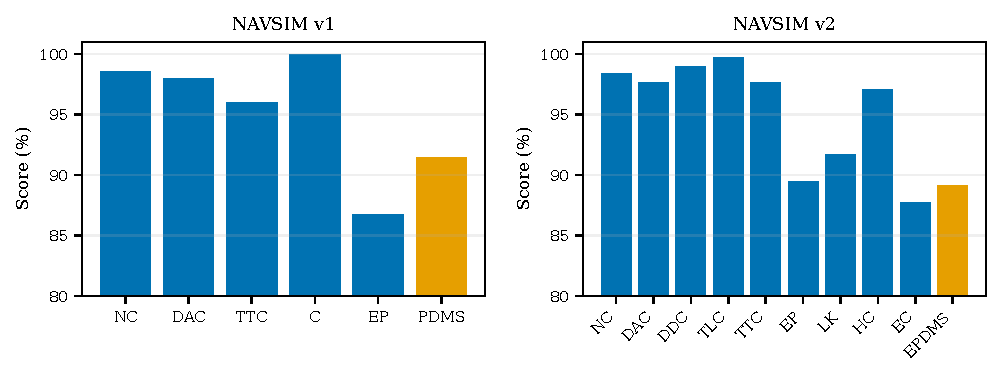
\includegraphics[width=0.76\textwidth]{figures/generated/ampt_metric_profiles.pdf}
  \caption{Scene-level reproduced AMPT component profiles on NAVSIM v1 and
  v2.  All metrics are percentages and higher is better; aggregate PDMS/EPDMS
  is shown in orange.  The profiles use 12,138 and 12,146 scored scenes,
  respectively, from one inference realization.}
  \label{fig:metric-profiles}
\end{figure*}

\paragraph{Single-trajectory inference.}
For each scene and inference seed, the model receives one observation, runs one
five-step denoising chain, and submits its single final $8\times3$ trajectory.
There is no test-time group sampling, evaluator call, candidate scoring,
reference lookup, model ensemble, or reranking.  The v1 submission provenance
independently records candidate count one, so this is a scene-level reproduced
property rather than only a methodological statement.

\paragraph{Runs and uncertainty.}
The archived v1/v2 headline exports each establish a scene-level mean for one
policy realization; they do not establish across-seed variance.  We therefore
do not attach a fabricated standard deviation to the 0.1--0.3 point increments
in the paper.  For the proposed rerun, each of seeds
20260726/20260727/20260728 produces a
complete scene export.  We first compute the mean for each run and report the
mean $\pm$ standard deviation across the three runs.  Method differences use
10,000 paired bootstrap resamples of shared scenes (resampling seeds and then
scenes within seed when multiple seeds are present), with a fixed analysis seed
of 2027 and a two-sided 95\% interval.  Recovery proportions use Wilson 95\%
intervals.  Scene bootstrap intervals from one model run describe variation
over the evaluated scenes and are explicitly not interpreted as training-seed
stability.

\paragraph{Model selection disclosure.}
The archived final v1 provenance states that \texttt{navtest} participated in
checkpoint selection.  We therefore describe the headline table as a
paper-reported benchmark comparison, not as a clean held-out model-selection
study.  The proposed rerun selects checkpoints only on the training/validation
partition, seals a checkpoint hash before \texttt{navtest}, and evaluates each
sealed hash once per inference seed.  This disclosure does not change a main
paper number; it narrows the fairness claim to what the available provenance
supports.

\subsection{The Fixed 658-Scene Recovery Protocol}
\label{sec:hard658-protocol}

The hard population is fixed before comparing optimization methods.  A scene
enters the set when the ReCogDrive IL policy receives PDMS zero in all five
sampling attempts because of collision, drivable-area violation, or both.
The resulting intersection contains 658 scene IDs.  A method \emph{recovers} a
scene when its single submitted trajectory has PDMS strictly greater than
zero under the same evaluator; the threshold is not retuned per method.

For consistency with the main paper, every supplementary hard-set analysis
uses the same archived scalar-GRPO versus historical Core-Pareto recovery pair that produced
367 and 440 positive-score scenes.  It does not substitute a later
full-benchmark checkpoint.  On the 658 fixed scenes, scalar GRPO has 367
positive and 291 zero-score outcomes, whereas the manuscript recovery
checkpoint has 440 positive and 218 zero-score outcomes.  Their paired
transition counts are 347 retained successes, 20 new failures, 93 repaired
failures, and 198 persistent failures.  Hence the net recovery is
$93-20=73$ scenes, exactly the change $440-367$, rather than a gain obtained by
hiding newly failed scenes.  The corresponding recovery rates are 55.8\%
(Wilson 95\% CI 52.0--59.5; $n=658$) and 66.9\% (63.2--70.4; $n=658$).  A
10,000-sample paired scene bootstrap gives an absolute difference of 11.1
percentage points with a 95\% interval of 8.1--14.3 points.
These intervals describe one archived checkpoint pair; no training-seed
identifier was retained for this hard-set export.

The fixed-set construction contains 480 DAC-only, 165 collision-only, and 13
joint collision-and-DAC cases according to the archived cause manifest.  The
same IDs and failure labels are used in all hard-set transition and case-table
analyses.  In particular, ``440 recovered'' means 440 positive outcomes on the
fixed original population; the transition table is required whenever the
claim is interpreted as a policy-to-policy improvement.

\subsection{Baseline and Controlled-Comparison Protocol}
\label{sec:baseline-protocol}

\input{tables/generated/baseline_protocol.tex}

AMPT's v1 and v2 rows are locally reproduced from scene-level outputs.  Other
headline baseline rows are values reported in the main paper and their cited
sources; no local checkpoint, common prediction export, or common seed manifest
was found for them.  They are consequently labeled \emph{reported}, not
\emph{reproduced}.  The table records backbone, sensor interface, training
data, number of inference candidates, and use of a test-time scorer whenever
the cited evidence establishes those fields.  An unavailable field is marked
``not established by the audited source'' rather than filled by analogy with
AMPT.

For the GT/Score/Pareto/PC-MTS comparison, the paper reports a shared
initialization, diffusion SFT loss, optimizer, epoch budget, scalar-GRPO
configuration, and evaluation protocol.  The controlled reproduction
additionally seals the candidate-source manifest, fixes the proposed non-GT
sampling probability, matches the accepted candidate count, draws one target
per scene-update, and uses the same three proposed training seeds.  For Scalar GRPO versus FF-PGRPO, all rollout
chains are generated from the same initialization and sampled with the same
seed before the credit function is changed.  For No APR versus Full APR, total
optimizer steps are matched by continuing the no-APR policy with retention
targets.  These are proposed control procedures until their launch manifests
and outputs exist; the main-paper point estimates remain labeled
paper-reported.

\subsection{Reproduction and Integrity Checks}
\label{sec:reproduction-checks}

The canonical dataset stores normalized scores, benchmark and split, method,
stage, variant, round, scene ID, seed when recorded, feasibility/failure
transitions, teacher status, and its source-file/key provenance.  Validation
checks expected scene counts, duplicate scene-method records, score ranges,
the benchmark aggregate formulas, paired scene sets, and failure-state logic.
Final tables and figures are generated from that dataset; a validation failure
stops manuscript generation.  The build manifest records the command, analysis
seed, package versions, Git revision, and SHA-256 hashes of inputs and outputs.
All raw result directories are read-only, and all derived files remain under
the supplementary directory.

\section{PC-MTS Analyses: Supervision--Optimization Alignment}
\label{sec:pcmts-analysis}

This section is needed because the quality of a supervision target and its
value for subsequent policy optimization are different quantities.  PC-MTS is
designed for the latter: it keeps a target only when its score, component-wise
trade-off, local feasibility, and proximity to the frozen learner's rollout
support are jointly acceptable.  We first examine the observed
imitation-to-optimization reversal, and then specify the controls required to
separate policy compatibility from candidate count and training budget.

\subsection{The observed supervision--optimization reversal}
\label{sec:pcmts-mismatch}

Table~\ref{tab:supervision_mismatch} restates the reported comparison from the
main paper and makes the change induced by the common scalar-GRPO stage
explicit.  Score and Pareto selection produce the two strongest imitation
checkpoints (87.2 and 87.5 PDMS), yet both deteriorate under the subsequent
optimizer.  In contrast, PC-MTS deliberately gives up 0.3--0.6 imitation
points relative to those selectors and improves by 4.2 points after the same
optimization stage.  GT supervision also improves, but finishes 0.8 points
below PC-MTS.  Thus, ranking target sets by imitation PDMS would select Pareto,
whereas ranking them by optimized PDMS selects PC-MTS.  This reversal is the
direct evidence for the mismatch claimed in the paper.

\input{tables/generated/supervision_mismatch.tex}

\begin{figure}[t]
  \centering
  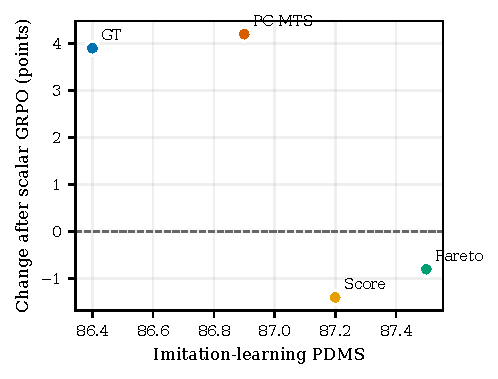
\includegraphics[width=\linewidth]{figures/generated/supervision_mismatch.pdf}
  \caption{Paper-reported imitation PDMS versus the change after the common
  scalar-GRPO stage on NAVSIM v1.  A high imitation score alone does not
  predict optimization value: Score and Pareto regress, whereas PC-MTS gains
  4.2 points.  Each marker is one reported point estimate; the paper does not
  state run/seed aggregation and no synthetic error bars are shown.}
  \label{fig:supervision-mismatch}
\end{figure}

The comparison should be interpreted at the level supported by the evidence.
It demonstrates that a higher-scoring imitation checkpoint need not be a
better starting distribution for GRPO, and that the PC-MTS set is compatible
with a large positive update in this run.  The archived paper table does not
contain scene-level outputs, acceptance counts, or multiple seeds for these
four cells.  Consequently, it does not by itself establish that the reversal
is invariant to seed, nor does it isolate candidate count from the four
filtering decisions.  We therefore do not attach synthetic error bars or
policy-distance values to these points.

\subsection{Candidate-count-matched reconstruction protocol}
\label{sec:pcmts-matched-protocol}

The released reproduction configuration turns the missing causal controls
into a predeclared, low-ambiguity experiment.  All four variants start from the
same GT-only checkpoint, use the same candidate sources, contribute exactly
one target per scene and update, train imitation learning for 200 epochs, and
then run scalar GRPO with 16 rollouts per scene for 10 epochs.  Within each
navigation-command/source stratum, accepted candidates are deterministically
subsampled to the smallest retained count across variants.  The non-GT
sampling probability is held fixed, so a method cannot receive more gradient
updates merely because it retains more candidates.  Empty strata fall back to
the logged trajectory.  In addition to final PDMS, a 300-update diagnostic
records the early GRPO gain before long-horizon training effects can dominate.

For a fully specified reconstruction when the original resolved PC-MTS
manifest is unavailable, the release marks the following as \emph{proposed
reproduction settings}, not measured settings of the reported run: a rollout
bank of 16, $K=3$ neighbors, a command-conditional 0.95 calibration quantile,
and eight temporally correlated local perturbations.  The rollout bank and
calibration queries are disjoint by construction.  Three predeclared training
seeds (20260726, 20260727, and 20260728) are used for the reconstruction, while
bootstrap seed 2027 is reserved for analysis and is never treated as an additional
training run.  These choices fill the executable configuration without
retroactively attributing unrecorded hyperparameters to the main-paper result.

For each run, the pipeline records retained candidates, acceptance rate,
candidate-source composition, feasible rollout rate, feasible high-quality
rate, all-infeasible-group rate, zero-score rate, the 10th percentile,
CVaR-10, 300-update gain, and final scalar-GRPO PDMS.  Method differences are
computed on identical scenes with a 10,000-resample paired bootstrap; means
and standard deviations are reported across the three training seeds.

\subsection{Filter attribution and sensitivity}
\label{sec:pcmts-components}

The component experiment is cumulative: (i) aggregate Score only, (ii) Score
plus the component-wise Pareto gate, (iii) the preceding gates plus calibrated
policy compatibility, and (iv) the full selector with local-feasibility
testing.  Counts are matched after each gate, rather than relaxing a stricter
gate to reach a target count.  This distinction matters: a matched count must
not reintroduce candidates that failed the mechanism being tested.  The
decisive diagnostic is not imitation PDMS alone, but whether adding a gate
raises feasible rollout density and converts the fixed-budget GRPO change from
negative to positive.

The companion sensitivity protocol varies one factor at a time: rollout-bank
size in $\{8,16,32\}$, $K$ in $\{1,3,5\}$, calibration quantile in
$\{0.90,0.95,0.975\}$, and perturbation count in $\{4,8,16\}$.  Compatibility
alternatives are compared at the same acceptance rate: candidate-to-GT
ADE/FDE, distance to the deterministic policy output, minimum rollout-bank
distance, average $K$-nearest distance, and command-calibrated $K$-nearest
distance.  These are evidence-bounded planned analyses: the release contains
their configurations and logging schema, but no unexecuted outcome is used to
support the paper's reported 91.1 PDMS.

Taken together, the existing reversal and the matched protocol close two
different parts of the argument.  The former establishes that isolated target
quality can disagree with downstream optimization value; the latter defines
the experiment needed to attribute that disagreement specifically to policy
compatibility rather than supervision quantity.

\section{FF-PGRPO Analyses: Feasibility Before Positive Credit}
\label{sec:ffpgrpo-analysis}

Aggregate reward can hide an unsafe trade: progress or comfort may increase
enough to give positive standardized advantage even when collision avoidance,
drivable-area compliance, or a protected reference metric regresses.  The
purpose of FF-PGRPO is therefore not merely to reshape the scalar score, but to
change which rollouts are eligible for positive credit.

\subsection{What the stage ablation establishes}
\label{sec:ffpgrpo-stage-ablation}

On NAVSIM v1, the no-stage baseline in the main ablation has 86.5 PDMS, 98.1
NC, 94.7 DAC, 94.2 TTC, and 80.9 EP.  Applying FF-PGRPO without PC-MTS reaches
91.0 PDMS, with 98.4 NC, 98.0 DAC, 95.8 TTC, and 85.93 EP.  With PC-MTS as the
initialization, FF-PGRPO reaches 91.1 PDMS, 98.5 NC, 98.0 DAC, 96.0 TTC, and
86.0 EP before APR.  The improvement is therefore not produced by sacrificing
the displayed hard-safety components for progress: DAC improves by 3.3 points
and TTC by 1.6 points in the FF-PGRPO-only row, while EP increases by 5.03
points.  These are paper-reported point estimates whose run/seed aggregation
is not stated, so the small 0.1-point
difference between the two FF-PGRPO rows is not presented as a stable gain.

\input{tables/generated/stage_ablation.tex}

This result is consistent with the proposed ordering---recover feasibility,
then optimize continuous quality---but an aggregate stage ablation cannot
directly reveal the sign of individual rollout credits.  The fixed hard-scene
transition in Section~\ref{sec:hard658} provides scene-level evidence, and the
instrumentation below defines the rollout-level test.

\subsection{Credit diagnostics}
\label{sec:ffpgrpo-credit-diagnostics}

For rollout $i$, let $A_i>0$ denote positive assigned advantage and let
$V_i=1$ denote a violation of any hard-feasibility, protected-reference, or
admissible-Pareto condition.  We report
\begin{equation}
  \mathrm{PCVR} =
  \frac{\sum_i \mathbb{1}[A_i>0]V_i}
       {\sum_i \mathbb{1}[A_i>0]},
  \label{eq:positive-credit-violation}
\end{equation}
and separately count reference-regressing and Pareto-dominated positive
credits.  A denominator of zero is reported as ``no positive credits,'' not as
zero violation.  FF-PGRPO's implementation makes a violating rollout
ineligible for positive credit and exposes assertions for this contract.  The
archived training run, however, does not contain the per-rollout trace needed
to quote an observed PCVR; we do not convert a code invariant into a fabricated
measured rate.

The stepwise mechanism ablation adds: (i) the hard feasibility gate, (ii) the
coherent-reference guard, (iii) the Pareto positive-credit gate, and (iv) the
all-infeasible recovery rule.  Every variant logs group state
(all-feasible/mixed/all-infeasible), feasibility rate, positive and negative
advantage means, PCVR, reference-regressing positive-credit rate,
dominated-positive-credit rate, zero-to-feasible repair, positive-to-zero
regression, and updates until the first feasible rollout.  The coherent
reference is always one executable trajectory.  The historical
component-wise envelope remains only as an ablation because combining the best
value of each metric from different trajectories may describe no realizable
plan and can make every sampled rollout appear to regress.

The low-cost diagnostic run uses the paper's group size of 16 and stops at 300
updates; the final run uses the reported 10 epochs.  All variants share the
same sampled rollout tensors when credit is recomputed offline, which makes
the initial credit-assignment comparison independent of policy drift.  New
training is required only for the subsequent learning curves and remains
disabled unless explicitly enabled.

\subsection{Hard-scene evidence for feasibility-first recovery}
\label{sec:ffpgrpo-hard-evidence}

The manuscript recovery checkpoint is evaluated on the same 658-scene set as
scalar GRPO.  Scalar GRPO produces a positive score in 367 scenes (55.8\%,
95\% Wilson CI 52.0--59.5\%), whereas the AMPT recovery checkpoint is positive
in 440 scenes (66.9\%, CI 63.2--70.4\%).  The comparison uses a single
trajectory per scene and neither method uses test-time sampling, scoring, or
reranking.  Crucially, the paired transition is not merely a difference of
gross counts: 93 scalar-GRPO zeros become positive, 20 scalar-GRPO positives
become zero, 347 successes are retained, and 198 failures persist.  Net
recovery is therefore $93-20=73$ scenes, or 11.1 percentage points.  A
10,000-resample scene-paired bootstrap (analysis seed 2027) gives a 95\% CI of
8.1--14.3 percentage points for this paired change.  This interval quantifies
scene variation for this fixed checkpoint pair; it does not replace missing
multi-seed training uncertainty.

The subset mean PDMS increases from 0.5101 to 0.6145.  The corresponding
component means change from 0.8381 to 0.8815 for NC, 0.7052 to 0.7781 for DAC,
0.7705 to 0.8161 for TTC, and 0.4956 to 0.5932 for EP; comfort increases from
0.9985 to 1.0000, while DDC changes from 0.9567 to 0.9521.  This last decrease
is why protected metrics must be reported next to aggregate recovery rather
than summarized as universal component-wise improvement.  The complete
transition and failure-type decomposition are given in
Section~\ref{sec:hard658}.

The aggregate ablation, paired hard-scene transition, and positive-credit
instrumentation serve complementary roles.  The first shows the overall stage
gain, the second verifies that recovery is net positive rather than purchased
entirely with new failures, and the third is the predeclared test of the
claimed credit-assignment mechanism.

\section{APR Analyses: Dynamic, Policy-Relative Teachers}
\label{sec:apr-analysis}

APR addresses a moving-target problem.  A trajectory that is a useful local
teacher for the current policy can become redundant after refinement, while a
previously distant candidate can enter the policy's compatible neighborhood.
The relevant question is therefore not whether additional optimization steps
help, but whether rebuilding and re-auditing the teacher set provides useful
targets while retaining already safe behavior.

\subsection{Round-wise behavior and protected components}
\label{sec:apr-rounds}

The main paper reports a monotonic sequence of 91.10, 91.21, 91.37, and 91.45
PDMS from Round 0 through Round 3, corresponding to gains of $+0.11$, $+0.16$,
and $+0.08$.  In the stage ablation, adding APR to the PC-MTS+FF-PGRPO policy
raises PDMS from 91.1 to 91.4 and EP from 86.0 to 86.7, while the displayed NC,
DAC, TTC, and comfort values remain 98.5, 98.0, 96.0, and 100, respectively.
This pattern is aligned with APR's design: local teacher updates increase
progress without visible regression in the protected components at the
reported precision.

Each round value is a reported checkpoint summary; its run/seed aggregation is
not stated.  No across-seed
standard deviation is available, and the 0.08--0.16 point increments are not
claimed to be independently significant.  Moreover, the archived experiment
history contains accepted and rejected branches rather than a single complete
three-round hash chain; the four values above are therefore treated as the
paper's round-level summary, not as permission to infer missing intermediate
measurements.

\input{tables/generated/apr_rounds.tex}

\begin{figure}[t]
  \centering
  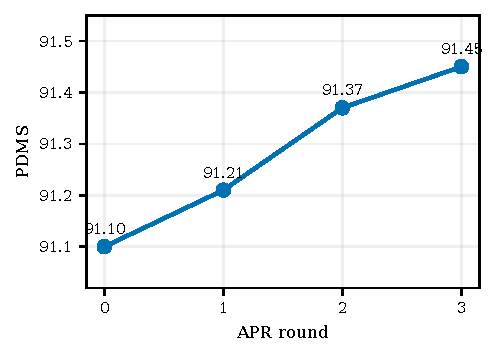
\includegraphics[width=\linewidth]{figures/generated/apr_rounds.pdf}
  \caption{Paper-reported NAVSIM v1 progression across APR rounds.  The final
  point is reproduced at scene level, but the small round increments are from
  one reported sequence and carry no across-seed error bar.}
  \label{fig:apr-rounds}
\end{figure}

\subsection{Teacher audit and post-interpolation evaluation}
\label{sec:apr-teacher-audit}

One traceable APR teacher-construction pass starts from 39,261 strict external
trajectories: 25,402 (64.7\%) from one driving-policy source and 13,859
(35.3\%) from a second source.  After interpolation with coefficient 0.25 and
exact re-evaluation, 28,910 targets remain, an acceptance rate of 73.6\%; the
remaining 10,351 are rejected.  These counts are from one audited navtrain
construction pass and are not presented as the source proportions of every
APR round.  They nevertheless establish an important operational fact:
interpolation is followed by evaluator-based admission, and the check is
non-vacuous---more than one quarter of the pre-audit union does not enter the
distillation set.

\input{tables/generated/apr_teacher_pool_audited.tex}

Teacher status is defined relative to the current policy.  A candidate is
\emph{accepted} when its evaluated local target is feasible, exceeds the
current single prediction by the required margin, preserves protected
metrics, and stays inside the current rollout neighborhood.  An accepted
teacher becomes \emph{expired} if it fails those tests after the policy is
updated.  A previously rejected candidate is \emph{newly activated} if it
passes after the rollout bank and current prediction are regenerated.  These
definitions prevent lifecycle counts from being conflated with raw pool size.

The interpolation search is descending: larger moves are evaluated first and
the first admissible move is retained.  Every accepted target stores the
teacher, current prediction, interpolation coefficient, post-interpolation
score, protected-metric deltas, compatibility distance, and evaluator hash.
No-interpolation and no-post-evaluation controls remove different safeguards:
the former jumps directly to the teacher, whereas the latter retains a local
trajectory without verifying that interpolation preserved feasibility.

\subsection{Step-matched controls}
\label{sec:apr-controls}

The release defines eight variants from the same Round-0 checkpoint and
matches the total number of optimizer updates: extra training on the existing
mixture, one-shot distillation, repeated use of a fixed teacher set, dynamic
teachers, dynamic teachers without interpolation, without post-interpolation
re-evaluation, without policy retention, and full APR.  The dynamic-teacher
and full-APR variants rebuild predictions, rollout banks, and teacher audits at
the same three round boundaries reported in the paper.  The fixed-teacher
variant repeats the Round-1 set without re-ranking it; the extra-training
control receives the same update count but no new teacher target.  This design
separates four possible explanations: more updates, teacher supervision in
general, teacher-set rebuilding, and the interpolation/retention safeguards.

For every round, the required report contains PDMS and all components,
regressed scenes, new failures, accepted/expired/newly activated teachers,
mean and median verified teacher advantage, interpolation-coefficient
distribution, and scene coverage.  A checkpoint is promoted only if its
single-trajectory aggregate score improves and protected metrics pass the
same non-regression audit; otherwise the previous checkpoint remains the
dynamic anchor.  Training ends after three promoted rounds or when no audited
local target remains.  These controls are configured but not represented as
measured results in this supplement, because running them would require new
training.

Optional task-vector consolidation is kept separate from teacher discovery.
The implementation can mask low-salience coordinates, require directional
agreement, bound each branch norm and the total displacement from the current
anchor, and then evaluate the merged checkpoint.  The best-branch, simple
average, task-arithmetic, and TIES-style controls are required before assigning
an independent gain to merging~\cite{taskarithmetic2023,ties2023}.  In the
absence of a stable, step-matched gain, merging should be read as a conservative
checkpoint-consolidation detail, not as the source of APR's teacher lifecycle.

The present evidence therefore supports two bounded statements: the reported
APR rounds are monotonic and preserve the displayed safety/compliance metrics,
and an audited construction pass materially filters proposed local targets
after re-evaluation.  The step-matched variants above are the necessary test
for the stronger causal claim that dynamic rebuilding, rather than additional
training alone, explains the full increment.

\input{tables/generated/apr_fixed_teacher_diagnostic.tex}

\section{Failure Recovery and Qualitative Diagnostics}
\label{sec:failure-qualitative}

Qualitative evidence is most useful when organized by a mechanism and tied to
scene-level metrics.  We therefore analyze the fixed hard set first, then give
traceable examples of recovered, persistent, and newly introduced failures.
All quantitative hard-set results and the mechanism-organized case table use
the same historical checkpoint pair as the main paper's 367-versus-440
recovery claim.  The final full-benchmark visualization is separately labeled
and is not used in the 658-scene recovery analysis.

\subsection{Construction of the fixed 658-scene set}
\label{sec:hard658}

The set contains 658 NAVSIM v1 scenes for which the initial ReCogDrive policy
obtained exactly zero PDMS in all five construction samples because of an
at-fault collision (NC), drivable-area violation (DAC), or both.  The set is
fixed before comparing the scalar-GRPO and AMPT recovery checkpoints.  Under
single-trajectory evaluation, scalar GRPO is positive on 367 and zero on 291
scenes; the AMPT recovery checkpoint is positive on 440 and zero on 218.

The paired $2\times2$ transition is
\begin{equation}
\begin{array}{c|cc|c}
 & \multicolumn{2}{c|}{\text{AMPT recovery checkpoint}} & \\
\text{scalar GRPO} & \text{zero} & \text{positive} & \text{row total} \\
\hline
\text{zero}     & 198 & 93  & 291 \\
\text{positive} & 20  & 347 & 367 \\
\hline
\text{column total} & 218 & 440 & 658
\end{array}.
\label{eq:hard658-transition}
\end{equation}
Hence 93 failures are repaired, 347 successes are retained, 198 failures
persist, and 20 new failures appear.  The net change is $93-20=73$, exactly the
difference between the gross positive counts $440-367$.  This distinction is
important: 440/658 is the gross recovery rate relative to the policy used to
construct the hard set, whereas 93 and 20 describe the paired transition from
scalar GRPO to the AMPT recovery checkpoint.  The resulting 11.1-percentage-
point paired improvement has a scene-bootstrap 95\% CI of 8.1--14.3 points
(10,000 resamples, seed 2027).  It is a net improvement rather than an exchange
of an equal number of old and new failures.

\input{tables/generated/failure_recovery.tex}
\input{tables/generated/failure_net_gain.tex}

\begin{figure}[t]
  \centering
  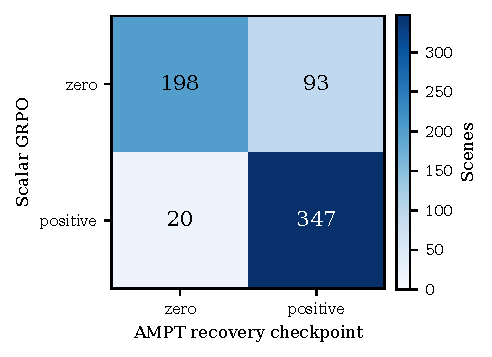
\includegraphics[width=\linewidth]{figures/generated/failure_transition.pdf}
  \caption{Scalar-GRPO to AMPT transition on the fixed 658-scene set.  The
  off-diagonal cells expose both 93 repairs and 20 regressions, rather than
  reporting gross recovery alone.}
  \label{fig:failure-transition}
\end{figure}

The original hard-set taxonomy contains 480 DAC-only scenes, 165 collision-
only scenes, 13 scenes failing both, and no residual ``other'' category.  The
paired repairs/new failures are 59/14 for DAC-only, 32/6 for collision-only,
and 2/0 for the joint category, giving net changes of 45, 26, and 2 scenes.
The gains are therefore not concentrated in only one failure type, although
the small joint category is descriptive rather than statistically decisive.

\input{tables/generated/failure_cause_breakdown.tex}

\begin{figure}[t]
  \centering
  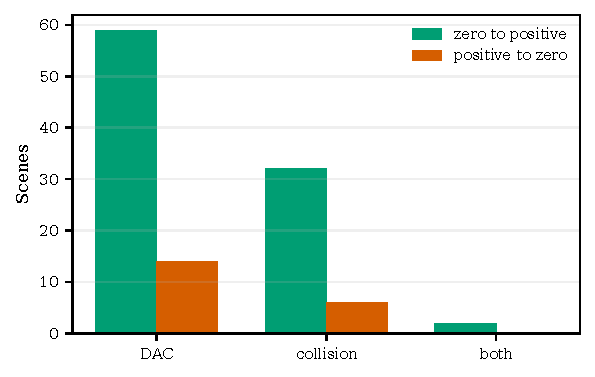
\includegraphics[width=\linewidth]{figures/generated/failure_cause_recovery.pdf}
  \caption{Repairs and regressions by the fixed hard-set cause taxonomy.  The
  net changes are 45 DAC, 26 collision, and 2 joint cases, totaling 73.}
  \label{fig:failure-causes}
\end{figure}

\subsection{Traceable scene cases}
\label{sec:traceable-cases}

Table~\ref{tab:hard658-cases} selects cases by transition type, not by visual
appeal.  Navigation commands come from the corresponding NAVSIM scene
metadata; scores and components come from the fixed paired evaluation.  The
table uses full scene identifiers so every row can be regenerated.  Component
pairs are scalar-GRPO $\rightarrow$ AMPT-recovery values.

\input{tables/generated/failure_cases.tex}

The first two cases are consistent with feasibility-oriented recovery: a hard
component changes from zero to one and positive PDMS returns.  Scene-level
before/after metrics do not identify the temporal order of training updates.
The third shows why ``recovered'' does not mean component-wise perfect.  The
fourth remains a DAC/progress failure under both audited checkpoints; without a
candidate/rollout manifest, the metrics do not identify whether pool coverage,
policy support, or optimization is responsible.  The fifth prevents
survivorship bias in the qualitative analysis and
motivates APR retention; it is one of the 20 positive-to-zero transitions
already charged against net recovery.

\subsection{Mechanism-centered visualization protocol}
\label{sec:qualitative-protocol}

The supplied renderer groups panels by decision rather than by scene
similarity.  A PC-MTS panel overlays an accepted candidate, a rejected distant
candidate, the logged trajectory, and the frozen-policy rollout neighborhood.
An FF-PGRPO mixed-group panel distinguishes unsafe, feasible-but-dominated,
and admissible Pareto-positive rollouts and prints their assigned advantages;
an all-infeasible panel shows the coherent recovery reference.  An APR panel
shows the current prediction, raw teacher, evaluated interpolant, and the
accepted/expired/newly-activated lifecycle state.  Every rendered panel reads
the scene id, command, component scores, and method name from its manifest and
uses a common legend: blue for the current prediction, green for an accepted
or positively credited trajectory, orange for a dominated/expired trajectory,
red for an unsafe trajectory, and black dashed for the coherent reference.

This protocol is also a safeguard against overinterpretation.  A camera/BEV
image is emitted only when the frame, command, all trajectories, and evaluator
record share the same scene identifier.  The metric-only cases in
Table~\ref{tab:hard658-cases} remain quantitative case studies if those visual
assets are unavailable; no unrelated camera frame or hand-drawn trajectory is
substituted merely to complete a panel.

\begin{figure*}[t]
  \centering
  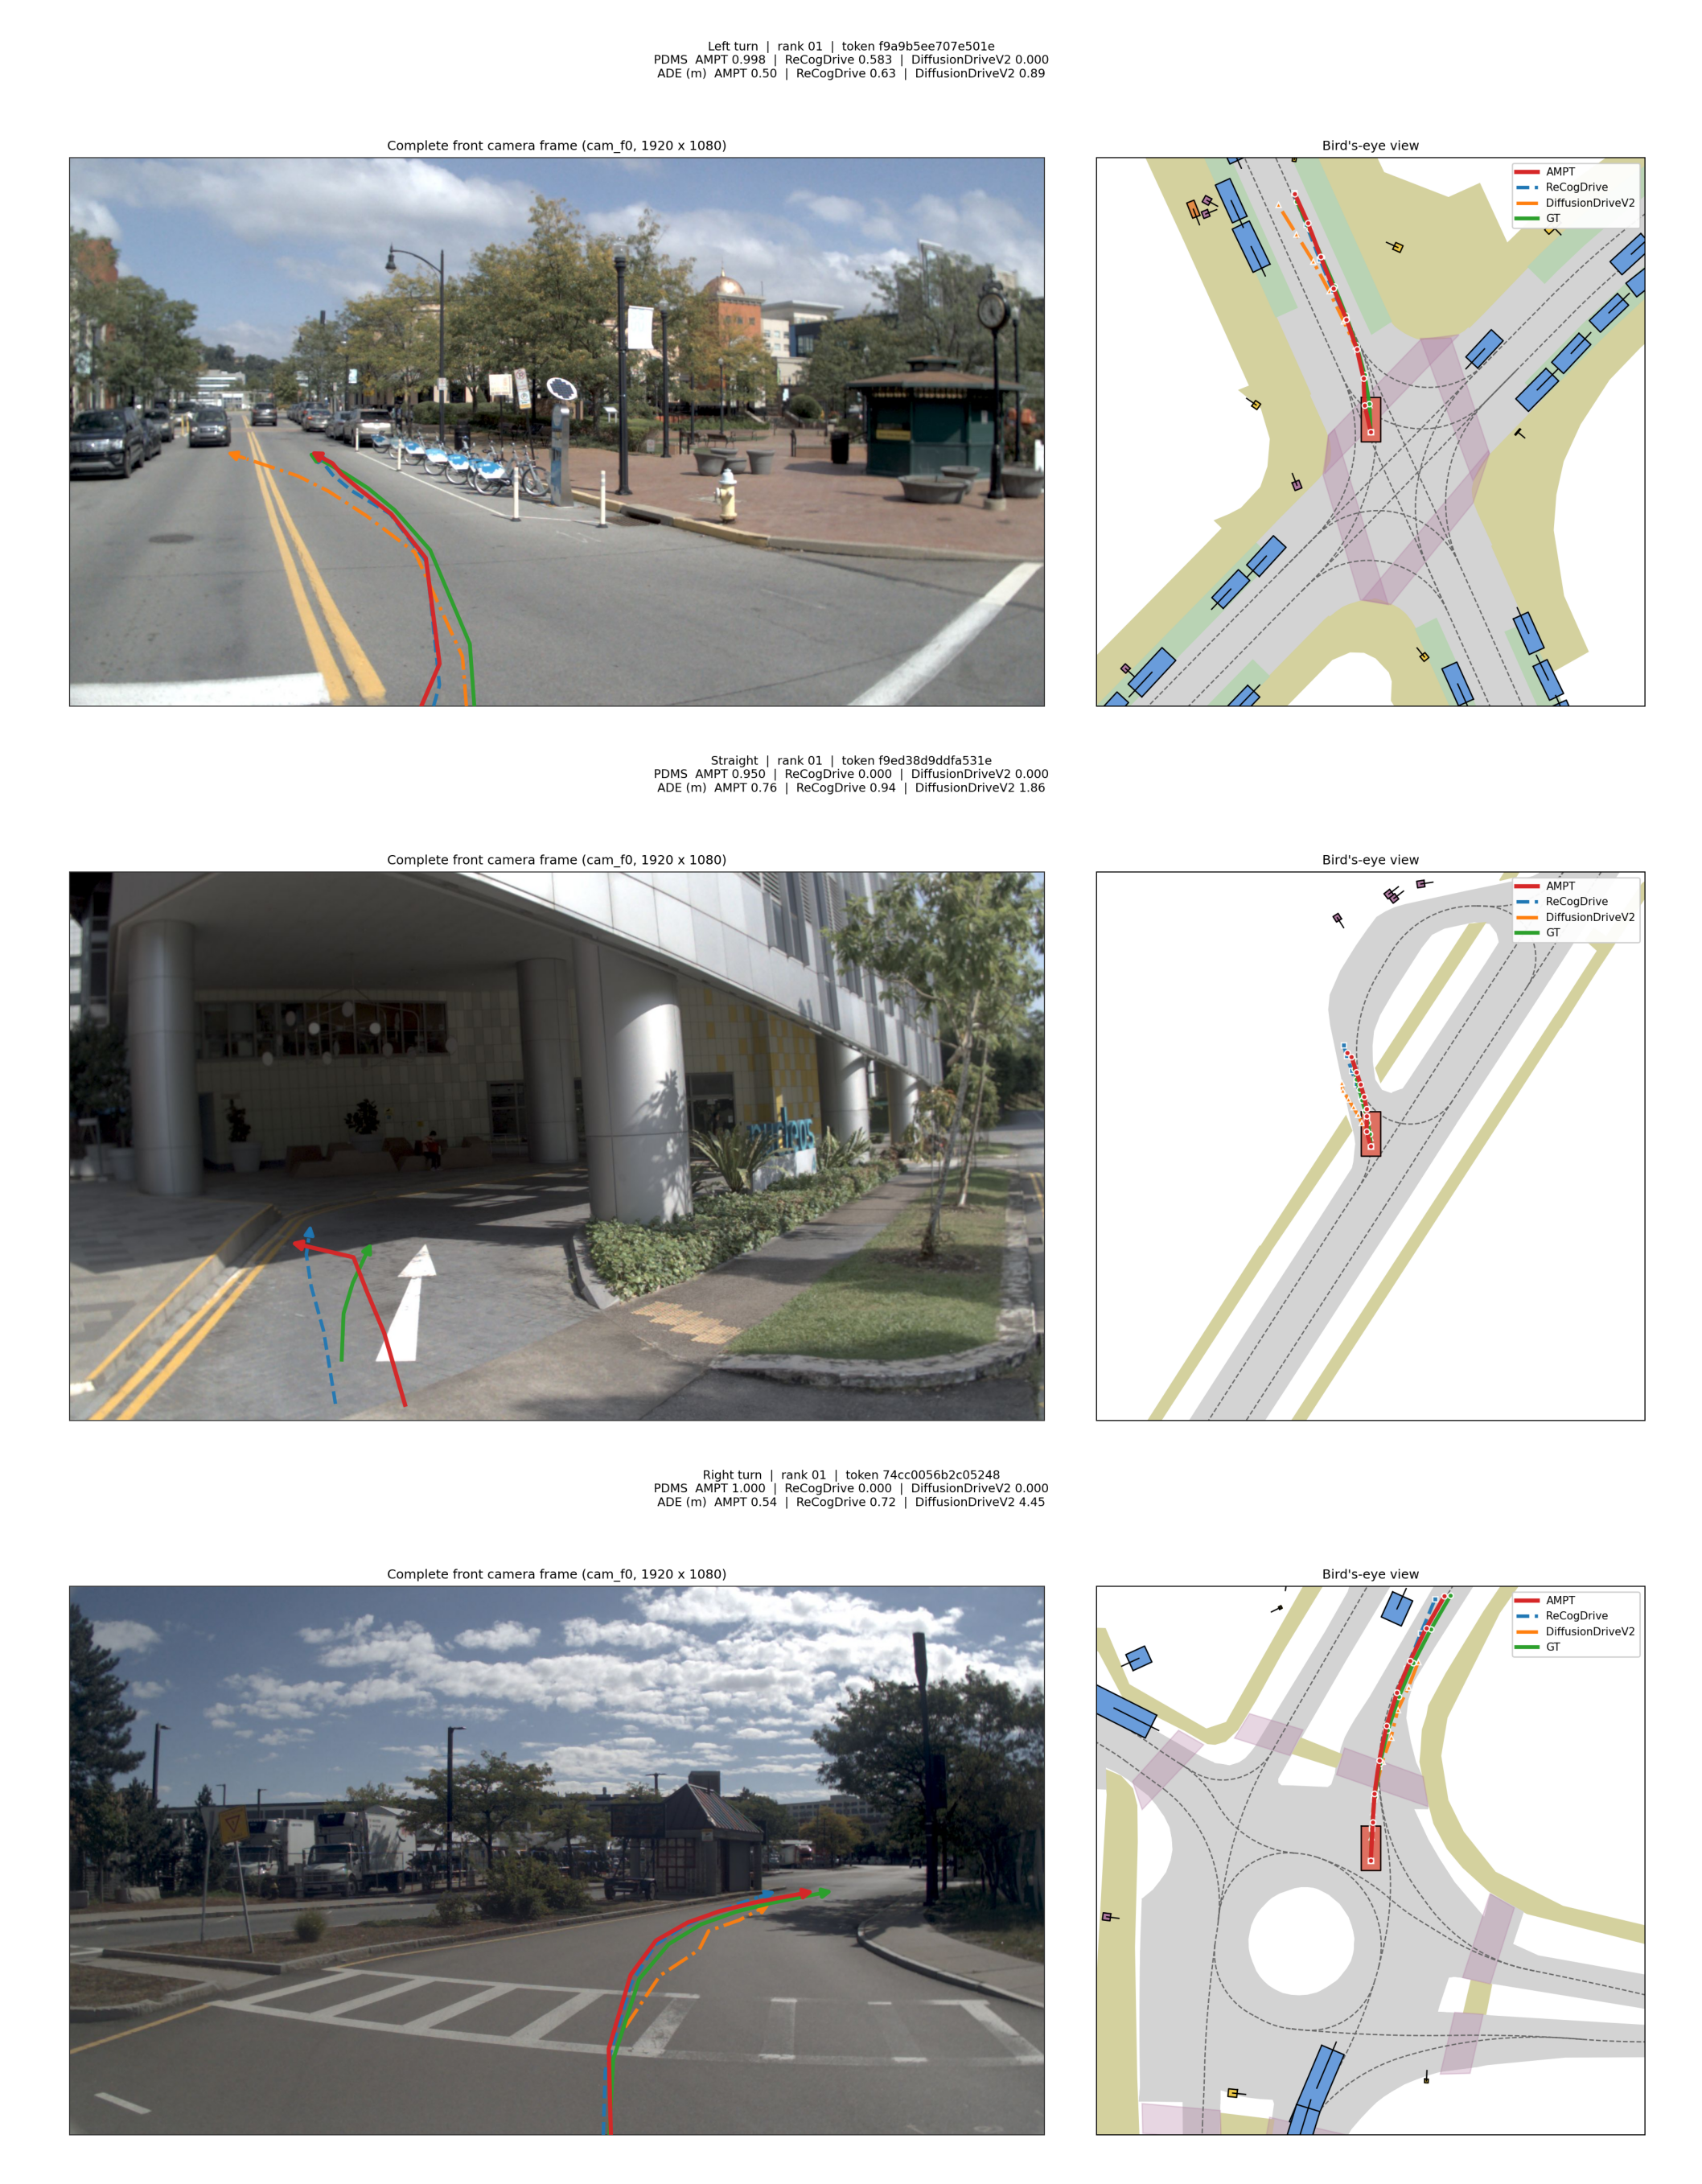
\includegraphics[width=0.92\textwidth]{figures/generated/qualitative_selected_cases.png}
  \caption{Three selected full-benchmark NAVSIM v1 cases (left, straight, and
  right commands) rendered from the separately audited final-AMPT manifest.
  Each row contains the complete front frame, bird's-eye view, scene ID,
  command, color legend, PDMS, and trajectory error.  These examples are not
  members of, and contribute no statistics to, the historical 658-scene
  recovery comparison; they illustrate final-policy behavior only.}
  \label{fig:qualitative-selected}
\end{figure*}

\clearpage

\section{Additional Related Work, Fair Comparison, and Limitations}
\label{sec:related-limitations}

\subsection{Related perspectives}

\textbf{Support-aware policy improvement.}
Conservative offline policy-improvement methods limit updates in regions where
the behavior data provide weak support.  SPIBB constrains uncertain decisions
to the baseline policy~\cite{spibb2019}, while BEAR regularizes a learned policy
toward the behavior distribution~\cite{bear2019}.  PC-MTS shares the support
intuition but applies it before optimization: it filters trajectory-level
supervision using samples from the frozen learner, with command-conditional
calibration and a local feasibility test.  It is not a general monotonic-
improvement guarantee; its role is to avoid moving the imitation policy into a
region where downstream rollout optimization has poor local support.

\textbf{Multi-objective and Pareto optimization.}
Multi-objective reinforcement learning studies policies under vector-valued
returns and alternative preference models~\cite{roijers2013}.  AMPT does not
seek a global set of Pareto-optimal policies.  PC-MTS uses a scene-local Pareto
filter for supervision, and FF-PGRPO uses a hierarchy: hard feasibility and
coherent-reference guards are evaluated before a rollout can receive positive
Pareto credit.  This order is essential when an aggregate score can compensate
for a protected regression.

\textbf{Advantage-weighted behavior learning.}
Advantage-weighted regression turns estimated advantages into weights for
supervised policy updates~\cite{awr2021}.  APR is related at the loss level,
but its weights are attached only after a candidate is compared with the
current single-trajectory prediction, locally interpolated, and re-evaluated.
Teacher admission and policy retention are therefore as important as the
weighting function itself.

\textbf{Model merging.}
Task arithmetic combines model displacements relative to a shared
anchor~\cite{taskarithmetic2023}, and TIES resolves redundancy and sign
conflicts before merging~\cite{ties2023}.  AMPT may use an anchor-constrained
variant to consolidate APR branches, but merging is optional and is separated
from teacher selection.  Passing parameter-space norm and sign checks does not
imply behavioral safety; every merged checkpoint must still undergo the same
single-trajectory evaluator audit.

\subsection{Fair-comparison boundary}
\label{sec:fair-comparison}

AMPT uses one predicted trajectory at inference.  Policy rollout banks,
candidate pools, coherent references, group sampling, specialist policies, and
the offline evaluator are training-only; there is no test-time scorer,
best-of-$N$ selection, or candidate reranking.  This contract is present in the
paper and is independently supported by the v1 submission provenance.

The released v1 scene export contains 12,138 successfully scored scenes from
12,146 predictions; the eight unscored predictions are disclosed rather than
imputed.  The v2 export contains 12,146 successful scene scores.  Its EC
aggregation follows the official evaluator, although a direct EC value is
present for 10,040 rows.  Scene-bootstrap intervals resample these scored
scenes and are explicitly labeled as scene uncertainty; they are not a
substitute for independent training runs.

The baseline rows in the main tables are treated as \emph{reported} unless a
local scene export and matching protocol are available.  AMPT's v1/v2 rows are
reproduced from scene-level outputs, but protocol matching is not established
for every external baseline.  Moreover, the audited v1 provenance records use
of navtest for checkpoint selection.  We therefore avoid a strict held-out
state-of-the-art claim and report protocol fields---backbone, sensors, training
data, inference candidates, and test-time scoring---alongside each comparison.

The 658-scene result uses the recovery checkpoint and checkpoint pair specified
by the main-paper analysis.  It is a fixed-subset diagnostic, not a claim that
every later checkpoint must induce the same transitions.  Reporting the full
$2\times2$ matrix in Eq.~\ref{eq:hard658-transition} makes the gross and net
notions of recovery explicit.

\subsection{Limitations}
\label{sec:limitations}

\textbf{Finite support estimates.}
Compatibility is estimated from a finite rollout bank.  Sparse commands or
multi-modal scenes can make a genuinely useful target appear distant, and the
calibrated neighborhood is only as representative as the frozen policy
samples.  Increasing bank size improves coverage but raises offline inference
and storage cost.

\textbf{Evaluator bias and non-reactive evaluation.}
All three stages use an offline NAVSIM evaluator for filtering, credit, or
teacher validation.  Systematic evaluator errors can therefore be amplified
across stages.  NAVSIM's non-reactive agents also cannot reveal how other road
users would respond to the learned trajectory; feasibility under this scorer
is not a closed-loop safety guarantee.

\textbf{Candidate-pool ceiling.}
APR can select and localize only behaviors represented in its multi-source
pool.  If no source proposes a valid maneuver, rebuilding the pool changes no
target.  The persistent case in Table~\ref{tab:hard658-cases} establishes
persistence under two audited checkpoints, but cannot diagnose this pool
ceiling without a per-scene candidate manifest.

\textbf{Locality can reject long-horizon value.}
The policy-compatibility filter intentionally favors learnable local targets.
It may reject a distant behavior that is initially difficult to imitate but
would be valuable after a longer curriculum.  Policy-dependent teacher-value
and cross-policy selection experiments are therefore important follow-ups.

\textbf{Benchmark-specific hierarchy.}
The ordering of NC/DAC feasibility, DDC/TLC guards, progress floors, and
continuous Pareto objectives reflects NAVSIM metrics.  Transferring AMPT to a
new benchmark requires revalidating the hierarchy and calibration thresholds,
not merely renaming metric fields.

\textbf{No behavioral semantics for parameter merging.}
Task-vector masks, direction agreement, and norm constraints bound parameter
movement but do not provide a semantic or safety guarantee.  If its independent
gain is not stable across seeds and step-matched controls, merging should
remain an implementation detail.

\textbf{Statistical scope.}
The supervision comparison, stage ablation, and APR round table are available
as reported point estimates rather than three-seed aggregates.  Small APR
increments must not be described as stable until the configured multi-seed
controls are run.  The paired 658-scene interval establishes a robust scene-
level net transition for one checkpoint pair, but does not measure training-
seed variation.

These limitations narrow rather than alter the paper's central claim.  The
currently traceable evidence establishes the supervision--optimization
reversal, a large feasibility-oriented stage gain, monotonic reported APR
rounds with preserved displayed safety components, and positive net recovery
on a fixed hard set.  Candidate-count matching, rollout-level credit traces,
step-matched APR controls, and multi-seed reruns are the remaining experiments
needed for stronger causal and stability claims.


\bibliographystyle{plain}
\bibliography{supplementary}
\end{document}
 to
% include only the appendix body from an existing manuscript preamble.
\ifdefined\AMPTMainPaper
  \makeatletter
  \def\input@path{{supplementary/}{supplementary/sections/}}
  \makeatother
  \graphicspath{{supplementary/}}
  \appendix
  \section{Additional Method Details}
\label{sec:additional-method}

This appendix makes explicit the contracts that connect the three training
stages.  This is important because the central claim of AMPT is not that a
trajectory with a high offline score is automatically a useful target, but
that supervision, rollout credit, and policy-relative refinement must agree on
what the current policy can safely learn.  We use three provenance labels
throughout.  \emph{Paper-reported} denotes a value stated in the main paper,
\emph{scene-level reproduced} denotes a value recomputed from an archived
per-scene evaluator export, and \emph{proposed reproduction} denotes a fully
specified setting for rerunning an experiment whose resolved training manifest
was not retained.  The last category is a protocol, not an observed result.

\subsection{Policy-Compatible Multi-Trajectory Supervision}
\label{sec:pc-mts-details}

\paragraph{Candidate construction and source balancing.}
For a scene $s$, let $\tau_s^0$ be the logged trajectory and let
$\mathcal C_s=\cup_m\mathcal C_s^{(m)}$ be the union of candidates supplied by
the configured proposal generators.  PC-MTS is source agnostic: a source may
be another policy seed, a structured trajectory expander, or a specialist
planner, but source identity is retained in the manifest and geometric near-
duplicates are merged before scoring.  The logged target is immutable and
is never removed.  A final Stage-1 source-count manifest was not found.  To
make the controlled reconstruction executable without presenting invented
counts as measurements, our \emph{proposed reproduction} caps every non-GT
source at eight candidates per scene before filtering.  When comparing Score,
Pareto, and PC-MTS, we use the same source
cap and retain the same number of non-GT candidates by taking the best valid
items under the corresponding rule.  Thus a difference cannot be attributed
to exposing one variant to a larger target set.

\begin{table*}[t]
\centering
\small
\caption{Candidate-source and audit budgets for PC-MTS on the NAVSIM training universe. Counts tagged proposed are reproduction settings rather than observations; higher/lower is not applicable.}
\label{tab:candidate_sources}
\resizebox{\textwidth}{!}{%
\begin{tabular}{lccccc}
\toprule
source & role & per\_scene\_budget & scene\_universe & retention\_or\_use & status \\
\midrule
Logged trajectory & immutable fallback and retention target & 1 & 103,288 expected navtrain scenes & always retained & paper-described / historical contract \\
Frozen-policy rollout bank & compatibility support estimate & 16 & 103,288-scene reproduction universe & distance calibration only & proposed reproduction setting \\
Multi-source candidate proposals & quality and Pareto targets & 8 per source & 103,288-scene reproduction universe & subject to quality/Pareto/compatibility gates & proposed reproduction budget \\
Correlated local perturbations & local feasibility audit & 8 per retained proposal & same candidate scenes & pass-rate threshold 0.75 & proposed reproduction setting \\
\bottomrule
\end{tabular}%
}
\end{table*}


\paragraph{Quality, feasibility, and Pareto filtering.}
Every complete trajectory is scored by the same offline evaluator used for
training diagnostics.  We first require hard feasibility, then a sufficient
aggregate score, and only then form the scene-wise component Pareto front.  A
candidate $a$ dominates $b$ only if it is no worse on every active Pareto
objective and is strictly better on at least one.  This order matters: a high
progress value cannot compensate for collision or leaving the drivable area.
The paper does not archive the numerical Stage-1 aggregate cutoff.  In the
\emph{proposed reproduction}, a training-split quantile is selected once so
that comparison variants are matched to the minimum retained count, followed
by a source-balanced top-$k$ tie break.  The sealed cutoff is applied
identically to all splits and is never used to synthesize a reported score.

The benchmark-specific partition is summarized below.  On NAVSIM v1, NC and
DAC are hard gates; DDC is protected; and EP, TTC, and comfort are optimized
inside the admissible region.  On NAVSIM v2, NC, DAC, DDC, and TLC are the
multiplicative compliance gates.  The historical metric adapter uses EP, TTC,
and a composite $Q=(\mathrm{LK}+\mathrm{HC}+\mathrm{EC})/3$ as its three
continuous Pareto axes; the official EPDMS report still exposes LK, HC, and EC
separately.  For binary scorer outputs the \emph{proposed reproduction}
requires a value of one up to $10^{-6}$.  The archived safety contract uses
reference-relative tolerances of $0.01$ for DDC/comfort and $0.02$ for TTC/EP;
TLC remains a hard v2 gate.  These are historical implementation values, not a
claim about the unresolved configuration of the paper checkpoint.

\begin{table}[t]
\centering
\small
\caption{NAVSIM v1/v2 metric partition used by PC-MTS and FF-PGRPO. Hard feasibility is tested before protected non-regression and Pareto quality.}
\label{tab:metric_partition}
\resizebox{\linewidth}{!}{%
\begin{tabular}{lcccc}
\toprule
benchmark & hard\_feasibility & protected\_guards & pareto\_quality & aggregate \\
\midrule
NAVSIM v1 & NC, DAC & DDC; non-regression in TTC and feasibility & EP, TTC, C & PDMS \\
NAVSIM v2 & NC, DAC, DDC, TLC & DDC/TLC feasibility; non-regression in TTC & EP, TTC, LK, HC, EC & EPDMS \\
\bottomrule
\end{tabular}%
}
\end{table}


\paragraph{Policy compatibility.}
Let $\mathcal R_s=\{\rho_j\}_{j=1}^{M}$ be rollouts sampled from the frozen
GT-only policy under the same command as the candidate.  We standardize
waypoint displacement with per-timestep, command-conditioned robust scales
fitted on the calibration split, and write the resulting trajectory distance
as $d(\tau,\rho)$.  The archived implementation additionally exposes final
displacement, heading, and velocity diagnostics, but the proposed controlled
comparison changes only the normalized waypoint statistic.  The compatibility
statistic is
\begin{equation}
 d_{\mathrm{PC}}(\tau,\mathcal R_s)
 =\frac{1}{K}\sum_{\rho\in\operatorname{NN}_{K}(\tau;\mathcal R_s)}
 d(\tau,\rho).
\end{equation}
The threshold $q_c$ is the command-specific quantile of leave-one-out policy
rollout distances on calibration scenes.  The archived code proves
leave-one-out calibration within each policy cloud, but its retained manifest
does not prove driving-log-level independence.  The proposed reconstruction
therefore enforces log-disjoint calibration and query scenes.  The paper states the general
$K$-nearest statistic but does not report $M$, $K$, or $q_c$.  The archived
implementation realizes the valid $K=1$ special case.  Our \emph{proposed
reproduction} uses $M=16$, $K=3$, and $q_c$ at the 95th percentile, with
command groups merged into a global fallback only when a command group has
fewer than 16 calibration observations.  This choice is also the center point
of the supplied sensitivity grid, rather than a retrospectively selected
result.

\paragraph{Local feasibility tube.}
Compatibility to one rollout neighborhood does not by itself establish that a
target is robust to small prediction errors.  For every candidate that passes
the previous gates, PC-MTS adds correlated perturbations to $(x,y,\psi)$ and
the implied velocity sequence.  The perturbations are sampled from normalized
policy residuals, smoothed over time, and projected back to the command-consistent
trajectory representation before exact re-evaluation.  This changes whole
trajectory segments rather than independently jittering waypoints.  The
archived implementation supports 16 or 32 perturbations; the \emph{proposed
reproduction} uses eight lower-cost perturbations, preserves the empirical
temporal covariance of policy residuals, and accepts a candidate when at least
six of eight perturbations pass
the hard feasibility gates and the protected guards.  The P1 configuration
evaluates 4/8/16 perturbations and does not tune the threshold on the test
split.

\paragraph{Target sampling and fallback.}
After filtering, the training set for scene $s$ is
$\mathcal T_s=\{\tau_s^0\}\cup\mathcal A_s$, where $\mathcal A_s$ contains
accepted candidates.  A training update draws exactly one target for the
scene, so scenes with many proposals do not receive larger gradients.  The
\emph{proposed reproduction} draws the logged target with probability $0.5$
and otherwise samples uniformly from $\mathcal A_s$; if $\mathcal A_s$ is
empty, it deterministically uses $\tau_s^0$.  Candidate identity is sampled
before the diffusion timestep, so all noisy versions in that update correspond
to a single coherent target.  Fine-tuning uses the same denoising objective as
GT-only training and produces $\pi_{\mathrm{initial}}$.

\paragraph{Implementation correspondence.}
The source-balanced builder and immutable-GT path are implemented at
\path{41a8613:navsim/agents/recogdrive/curriculum/builder.py}
and \path{41a8613:navsim/agents/recogdrive/curriculum/proposals.py}.
Physical distance and calibrated reachability are at
\path{41a8613:navsim/agents/recogdrive/curriculum/reachability.py};
the feasibility and correlated-perturbation checks are at
\path{41a8613:navsim/agents/recogdrive/curriculum/safety.py} and
\path{41a8613:navsim/agents/recogdrive/curriculum/robustness.py}.
These are historical mechanism-level implementations; the audit does not claim
that this commit is a complete hash-identical release of the final checkpoint.

\subsection{Feasibility-First Pareto GRPO}
\label{sec:ff-pgrpo-details}

\paragraph{A coherent scene reference.}
FF-PGRPO compares a rollout with one executable reference trajectory, never
with an envelope assembled from different trajectories.  The ordered source
set is: the logged trajectory, a retained PC-MTS candidate, and the current
single-trajectory prediction.  The paper-level rule selects the highest-scoring
feasible row.  The audited historical selector makes this precise by ranking
validity, hard feasibility, reference guard, robustness, core eligibility,
PDMS, distance to the current prediction, and source priority lexicographically.
Thus no higher score can bypass an earlier safety/eligibility tier.  If none is feasible, the
logged trajectory is retained only as a weak recovery target when it passes
the evaluator's basic physical checks.  Otherwise no recovery target is used
and every sampled rollout receives non-positive credit.  A component-wise
envelope is invalid because its NC, progress, and TTC values may come from
mutually incompatible plans; positive credit relative to such a synthetic
point would have no executable safety witness.

\paragraph{Group states and admissibility.}
For each scene the paper reports a group of $G=16$ policy rollouts.  We assign
the group to one of three states.  An \emph{all-feasible} group contains only
rollouts that satisfy hard feasibility; its quality statistic normalizes the
continuous score components because the binary gates are constant.  A
\emph{mixed} group contains both feasible and infeasible rollouts; feasibility
is applied first and feasible trajectories must additionally pass the coherent
reference guards.  An \emph{all-infeasible} group contains no feasible
rollout; it is not allowed to create a positive advantage by merely ranking
unsafe samples against one another.

For NAVSIM v1, admissibility requires NC and DAC and protects DDC, TTC, and an
EP floor relative to the coherent reference.  NAVSIM v2 additionally treats
DDC and TLC as hard compliance checks.  The archived safety-contract defaults
use $\mathrm{DDC}(\tau)\geq\mathrm{DDC}(r)-0.01$,
$\mathrm{TTC}(\tau)\geq\mathrm{TTC}(r)-0.02$, and
$\mathrm{EP}(\tau)\geq\mathrm{EP}(r)-0.02$.  The joint EP--TTC guard prevents
the optimizer from receiving positive credit for increasing safety merely by
stopping, or for increasing progress by collapsing the collision margin.

\paragraph{Credit assignment.}
Within a group that contains a feasible rollout, let $\widehat A_i$ be a
quality-shaped, group-relative score and let $P_i$ indicate membership in the
admissible Pareto front.  FF-PGRPO assigns
\begin{equation}
 A_i=\begin{cases}
 \max(\widehat A_i,0),
   & \substack{\text{feasible, guard-passing,}\\\text{and Pareto-positive}},\\
 \min(\widehat A_i,0),
   & \substack{\text{feasible but not}\\\text{admissible Pareto}},\\
 -\lambda_{\mathrm{unsafe}}+\min(\widehat A_i,0),
   & \text{infeasible}.
 \end{cases}
\end{equation}
Thus aggregate quality controls magnitude, whereas feasibility, a coherent
reference, and non-domination control the sign.  For mixed groups the quality
term also includes the EP-floor and joint EP--TTC penalties.  The historical
implementation preserves signs with RMS scaling rather than mean centering and
uses an archived default clip of $[-3,3]$; the \emph{proposed reproduction}
uses the predeclared sensitivity setting $[-5,5]$.

For an all-infeasible group, violation severity is the normalized sum of hard
gate deficits and protected-metric deficits.  Credit is the non-positive
within-group rank of negative severity, shifted by the unsafe penalty.  The
group loss is downweighted to $0.25$; when a valid recovery reference exists,
a diffusion recovery term with coefficient $0.25$ is added.  The proposed
regularization uses KL weight $0.02$ and anneals the BC coefficient linearly
from $0.10$ to $0.05$ over the first five epochs.  These numerical values are
historical implementation defaults and proposed rerun values, not recovered
resolved parameters for the paper's final FF-PGRPO run.

\paragraph{Diffusion credit and inference.}
One trajectory-level advantage is broadcast to every transition in that
trajectory's denoising chain.  The audited planner uses a discounted
transition-wise mean, while the paper objective writes the chain likelihood in
accumulated form; the proposed reconstruction preserves the planner reduction
and logs it in the resolved manifest.  This avoids assigning mutually
inconsistent metric credit to intermediate noisy states that are not executable
plans.  At inference, AMPT runs one denoising chain and emits one trajectory.
Group sampling, the Pareto computation, the reference selector, the offline
evaluator, and candidate reranking are absent from test time.

\paragraph{Implementation correspondence.}
Group classification, Pareto gating, violation ranking, sign-preserving
normalization, and clipping are at
\path{41a8613:navsim/agents/recogdrive/stage3_ff_pareto.py}.
The coherent-row API is at
\path{41a8613:navsim/agents/recogdrive/stage3_reference_selector.py},
and positive-credit assertions are at
\path{41a8613:navsim/agents/recogdrive/stage3_positive_credit_contract.py}.
The archived tensor layout is anchor-local; the paper-level protocol is the
union of 16 scene rollouts.  Because a final resolved layout manifest was not
found, we do not infer the number of anchors from a class default.

\subsection{Adaptive Pareto-Guided Policy Refinement}
\label{sec:apr-details}

\paragraph{Dynamic multi-source pool.}
At APR round $r$, the current policy $\pi_r$ supplies one local prediction for
every scene.  Candidate teachers come from historical policy checkpoints,
independent GRPO seeds, structured trajectory expansion, and safety-,
progress-, and regularity-oriented specialists.  Source labels survive
deduplication so per-source acceptance can be audited, but final three-round
source proportions were not archived.  The audited initial construction keeps
its observed 25,402/13,859 source mixture.  The proposed source-ablation reports
each source separately instead of claiming an unrecorded balancing rule.

\paragraph{Teacher audit.}
For a policy prediction $p_s$ and candidate teacher $t$, APR first requires
feasibility and an aggregate margin $R(t)-R(p_s)\geq m_R$.  It then applies
absolute and reference-relative protected guards.  Behavioral distance,
curvature, and jerk rank otherwise admissible teachers; they are preferences,
not claimed historical hard thresholds.  In the audited APR branch,
$m_R=0$ with a strict positive comparison, DDC has absolute floor 0.99 and
maximum drop 0.01, TTC has absolute floor 0.95 and maximum drop 0.02, and the
jerk coefficient 0.005 is a soft training regularizer.  At the interpolation
audit, the proposed reconstruction additionally applies the command-conditioned
95th-percentile compatibility calibration from PC-MTS.

\paragraph{Local interpolation and exact re-evaluation.}
An accepted teacher is not copied directly.  APR evaluates
\begin{equation}
 \tau_{s,\alpha}=p_s+\alpha(t-p_s)
\end{equation}
for a descending list of interpolation coefficients.  The first (largest)
coefficient that remains feasible, improves the aggregate score, preserves
protected metrics, and passes the current compatibility test becomes the local
target.  Every interpolated trajectory is scored anew; endpoint scores are
never linearly interpolated.  One audited branch used $\alpha=0.25$.  The
\emph{proposed reproduction} fixes the descending list to
$[1.0,0.75,0.50,0.25]$, which includes that audited setting and tests the
teacher endpoint before progressively more conservative steps.  If all
coefficients fail, the teacher is
rejected for the current round rather than kept with a smaller unscored step.

\paragraph{Weighted distillation, retention, and lifecycle.}
For verified gain $\Delta_s=R(\tau_{s,\alpha})-R(p_s)>0$, the target weight is
\begin{equation}
 w_s=\min\{5,\exp(\Delta_s/0.05)\}.
\end{equation}
The temperature $0.05$ and clip 5 are present in an audited APR training
branch.  The same diffusion denoising loss is applied to weighted local
targets, while current predictions provide retention targets with audited
weight 1.0.  At most the top one positive-advantage target is used per scene; a
scene without a valid teacher contributes retention only.  After training, the
candidate checkpoint is promoted only if aggregate validation score increases
and none of the protected aggregate components regresses beyond the audit
tolerances.  The promoted checkpoint becomes the dynamic anchor, its
predictions and rollout bank are regenerated, and the complete teacher pool is
audited again.  A previously accepted teacher is defined as \emph{expired} when
it loses its margin or guard, while a previously rejected one is \emph{newly
activated} when it passes under the new policy.  Historical scripts rebuild
round files but do not persist these labels; the proposed pipeline obtains them
by joining teacher hashes across consecutive round manifests.  The paper reports three
rounds.  The proposed stop rule is the earlier of three promotions, an empty
teacher set, or no checkpoint passing the promotion rule; it does not turn a
small unverified score fluctuation into a promotion.

\paragraph{Optional branch consolidation.}
Safety, progress, and regularity branches may be consolidated after their
teacher updates.  This is an optional checkpoint operation, not a substitute
for teacher auditing.  The audited anchor-constrained variant keeps the top
20\% salient coordinates of each base-relative task vector, removes
coordinates with inconsistent directions, clips every branch displacement to
the norm of its accepted branch, and caps total displacement at $1.05$ times
the largest accepted branch displacement.  The anchor is the current promoted
policy and is therefore updated across rounds.  If no merge candidate passes
the same evaluation guard as an ordinary APR checkpoint, the best accepted
single branch is retained.

\paragraph{Implementation correspondence.}
Teacher audits are implemented at
\path{fb96a03:scripts/stage3/build_pdms_strict_teacher_buffer.py}
and \path{fb96a03:scripts/stage3/build_pdms_safety_repair_teacher_buffer.py}.
Interpolation and exact rescoring are at
\path{ab9124c:scripts/stage3/build_pdms_blended_teacher_reference.py},
with local safety-tube checks at
\path{ab9124c:scripts/stage3/filter_pdms_teacher_reference_by_safety_tube.py}.
Retention schedules are built by
\path{fb96a03:scripts/stage3/build_pdms_teacher_refinement_schedule.py},
and the optional merge is at
\path{64f5531:scripts/stage3/merge_conflict_free_anchored_task_vector.py}.
APR is an orchestrated sequence of these audited operations; the repository
does not contain a single monolithic \texttt{APR.run} entry point.

  \section{Algorithms}
\label{sec:algorithms}

The three procedures below are separated deliberately.  PC-MTS constructs a
supervision distribution before policy optimization; FF-PGRPO assigns credit
inside one rollout group; and APR rebuilds policy-relative teachers between
training rounds.  Combining them into one loop would obscure both their
different inputs and the interfaces tested by the implementation.  A code
comment names the closest audited historical function; ``paper contract''
marks a step for which no end-to-end final-checkpoint call graph was retained.

\paragraph{Algorithm 1: Policy-Compatible Multi-Trajectory Supervision.}
\label{alg:pcmts}
\begin{quote}
\small
\textbf{Input:} logged scenes $\mathcal D=\{(o_s,\tau_s^0,c_s)\}$; candidate
sources $\{\mathcal C_s^{(m)}\}$; frozen GT policy $\pi_{\mathrm{GT}}$;
offline evaluator $E$; compatibility and robustness configuration $\xi$.

\textbf{Output:} accepted per-scene target sets $\{\mathcal T_s\}$ and the
initialized policy $\pi_{\mathrm{initial}}$.

\begin{enumerate}
  \item Load source manifests, preserve source identity, form
  $\mathcal C_s=\cup_m\mathcal C_s^{(m)}$, merge geometric near-duplicates,
  and mark
  $\tau_s^0$ immutable.  \emph{Implementation:}
  \path{41a8613:navsim/agents/recogdrive/curriculum/proposals.py:load_scene_proposals},
  \path{deduplicate_proposals}; immutable retention is enforced by
  \path{builder.py:finalize_scene_record}.

  \item Evaluate every complete candidate with $E$; reject candidates that
  fail hard feasibility, the aggregate-quality threshold, intent checks, or
  reference-relative protected guards.  \emph{Implementation:}
  \path{41a8613:navsim/agents/recogdrive/curriculum/builder.py:build_scene_intermediate},
  \path{safety.py:absolute_feasibility} and
  \path{relative_nonregression}.

  \item Compute the component-wise Pareto front among survivors and apply the
  fixed source/role quota.  Do not allow a continuous metric to restore a
  candidate removed by a hard gate.  \emph{Implementation:} component-wise
  Pareto filtering is the paper contract; the audited tree exposes the later
  role/quota step at
  \path{41a8613:navsim/agents/recogdrive/curriculum/quota_selector.py:role_aware_quota_select},
  but no separately named Pareto-front function.

  \item Sample the policy rollout cloud $\mathcal R_s$ from frozen
  $\pi_{\mathrm{GT}}$.  Fit robust distance scales and command-specific
  quantiles using leave-one-out rollout queries.  Enforce log-disjoint
  calibration/query scenes in the proposed rerun; the archived manifest proves
  leave-one-out only.  \emph{Implementation:}
  \path{41a8613:navsim/agents/recogdrive/curriculum/builder.py:_policy_cloud_for_scene},
  \path{reachability.py:fit_reachability_calibration}.

  \item For each Pareto survivor $\tau$, compute its calibrated nearest-policy
  distance $d_{\mathrm{PC}}(\tau,\mathcal R_s)$ and retain it only when the
  relevant command threshold is met.  The archived branch implements $K=1$;
  the proposed rerun sets $K$ through $\xi$.  \emph{Implementation:}
  \path{41a8613:navsim/agents/recogdrive/curriculum/reachability.py:physical_distance_components},
  \path{evaluate_reachability}.

  \item Draw temporally correlated residual trajectories around every
  compatibility-passing candidate, score each perturbation with $E$, and keep
  the center candidate only if the required fraction remains feasible and
  guard-passing.  \emph{Implementation:}
  \path{41a8613:navsim/agents/recogdrive/curriculum/robustness.py:CorrelatedErrorModel.sample_perturbations},
  \path{evaluate_robustness_tube}.

  \item Set $\mathcal T_s=\{\tau_s^0\}\cup\mathcal A_s$.  If no non-GT
  candidate survives, set $\mathcal T_s=\{\tau_s^0\}$; never borrow a target
  from another scene.  \emph{Implementation:}
  \path{41a8613:navsim/agents/recogdrive/curriculum/builder.py:finalize_scene_record}.

  \item At each visit to $s$, sample exactly one member of $\mathcal T_s$
  according to the fixed GT/candidate mixture and then sample one diffusion
  timestep.  \emph{Implementation:}
  \path{41a8613:navsim/agents/recogdrive/stage2_role_sampler.py},
  \path{stage2_bridge.py}.

  \item Fine-tune a copy of $\pi_{\mathrm{GT}}$ with the unchanged diffusion
  noise-prediction loss and return it as $\pi_{\mathrm{initial}}$.
  \emph{Implementation:}
  \path{41a8613:navsim/agents/recogdrive/first_drive_v7_planner.py}.
\end{enumerate}
\end{quote}

\paragraph{Algorithm 2: Feasibility-First Pareto GRPO Credit Assignment.}
\label{alg:ffpgrpo}
\begin{quote}
\small
\textbf{Input:} scene $o_s$; policy $\pi_\theta$; the paper's $G=16$ sampled
denoising chains and final trajectories $\{(z_i,\tau_i)\}_{i=1}^{G}$; logged,
retained, and current-policy reference candidates; evaluator $E$; credit
configuration $\zeta$.

\textbf{Output:} trajectory advantages $\{A_i\}$ and the regularized
FF-PGRPO loss.

\begin{enumerate}
  \item Convert exact evaluator outputs for every $\tau_i$ to hard-feasibility,
  continuous-quality, protected-guard, and violation-severity tensors.
  \emph{Implementation:}
  \path{41a8613:navsim/agents/recogdrive/stage3_metric_adapter.py}.

  \item Rank complete logged, retained, and current-policy rows
  lexicographically by validity, hard feasibility, reference guard,
  robustness, core eligibility, PDMS, distance, and fixed source priority;
  choose the first row $r_s$.  Never take a different trajectory for each
  reference component.  Record whether a safe recovery reference is
  available.  \emph{Implementation:}
  \path{41a8613:navsim/agents/recogdrive/stage3_reference_selector.py:CoherentReferenceSelector.select},
  \path{gather_reference_rows}.

  \item Classify the rollout group as \textsc{all-safe}, \textsc{mixed}, or
  \textsc{no-safe}.  For safe rollouts, evaluate coherent-reference guards and
  admissible Pareto membership.  The audited function consumes anchor-local
  $[B,K,R]$ tensors; the final $K\times R$ layout is unresolved, so the proposed
  rerun seals $K=8,R=2$ to preserve $G=16$.  \emph{Implementation:}
  \path{41a8613:navsim/agents/recogdrive/stage3_ff_pareto.py:classify_group_state},
  \path{anchor_local_pareto}.

  \item If the state is \textsc{all-safe}, form $\widehat A_i$ from only the
  continuous score terms.  If it is \textsc{mixed}, form $\widehat A_i$ from
  aggregate quality plus EP-floor and joint EP--TTC shaping.  Preserve the
  scene grouping during normalization.  \emph{Implementation:}
  \path{41a8613:navsim/agents/recogdrive/stage3_ff_pareto.py:FeasibilityFirstCreditAssigner.compute}.

  \item For an \textsc{all-safe} or \textsc{mixed} group, set positive credit
  only for safe, guard-passing, Pareto trajectories; clamp safe dominated or
  guard-failing trajectories to non-positive credit; and apply an additional
  unsafe penalty to infeasible trajectories.  \emph{Implementation:}
  \path{41a8613:navsim/agents/recogdrive/stage3_ff_pareto.py:FeasibilityFirstCreditAssigner.compute}.

  \item For a \textsc{no-safe} group, rank negative violation severity and
  assign only non-positive credit.  Downweight the group and, if $r_s$ is a
  valid recovery reference, add weak diffusion supervision toward $r_s$.
  \emph{Implementation:}
  \path{41a8613:navsim/agents/recogdrive/stage3_ff_pareto.py:FeasibilityFirstCreditAssigner.compute};
  the exact final recovery-loss integration is not retained.

  \item Apply sign-preserving RMS scaling and symmetric clipping.  Assert that
  no positive-credit rollout is infeasible, dominated, reference-regressing,
  or drawn from a no-safe group; log both numerator and denominator of every
  violation rate.  \emph{Implementation:}
  \path{41a8613:navsim/agents/recogdrive/stage3_ff_pareto.py:rms_scale_without_mean_centering},
  \path{stage3_positive_credit_contract.py:assert_positive_credit_contract}.

  \item Broadcast $A_i$ over the transitions of chain $z_i$, compute the
  planner's discounted transition-wise mean, and optimize it with KL/BC and
  optional recovery losses.  No evaluator or group operation is exported to
  inference.  \emph{Implementation:} the historical transition reduction is in
  \path{41a8613:navsim/agents/recogdrive/first_drive_v7_planner.py}; the audited
  commit does not expose a verified end-to-end call from that planner to
  \path{FeasibilityFirstCreditAssigner}.
\end{enumerate}
\end{quote}

\paragraph{Algorithm 3: Adaptive Pareto-Guided Policy Refinement.}
\label{alg:apr}
\begin{quote}
\small
\textbf{Input:} FF-PGRPO policy $\pi_0$; multi-source teacher pool
$\mathcal P$; evaluator $E$; interpolation list $\mathcal L$; number of rounds
$R=3$; audit and promotion configuration $\eta$.

\textbf{Output:} promoted single-trajectory policy $\pi_R$ and a round-wise
teacher lifecycle manifest derived by joining teacher hashes.

\begin{enumerate}
  \item At round $r$, run $\pi_r$ once on every training scene and cache the
  prediction, score components, trajectory geometry, and rollout-neighborhood
  calibration as the dynamic anchor.  \emph{Implementation:} policy inference
  and evaluator exports precede
  \path{fb96a03:scripts/stage3/build_pdms_teacher_refinement_schedule.py:make_refinement_schedule},
  which consumes rather than creates those cached predictions.

  \item Load and deduplicate candidates from historical policies, independent
  GRPO seeds, structured expansion, and safety/progress/regularity specialists.
  Retain source and trajectory hashes in every record.  \emph{Implementation:}
  \path{ab9124c:scripts/stage3/build_pdms_external_safety_repair_teacher_buffer.py:choose_external_safety_teachers}.

  \item Relative to the current prediction, reject a candidate unless it is
  feasible, clears the score margin, and preserves protected metrics.  Rank
  survivors by verified gain and then by smaller behavioral distance,
  curvature, and jerk; select at most one teacher for the scene.  These last
  quantities are preferences, not claimed historical hard gates.
  \emph{Implementation:}
  \path{fb96a03:scripts/stage3/build_pdms_strict_teacher_buffer.py:_strict_teacher_upgrade},
  \path{build_teacher_record}.

  \item For the selected teacher $t_s$, test
  $p_s+\alpha(t_s-p_s)$ in descending $\alpha\in\mathcal L$.  Score every
  interpolation with $E$ and choose the largest one that remains feasible,
  improves score, preserves guards, and remains policy compatible.  If none
  passes, create no teacher target for $s$.  \emph{Implementation:} the audited
  script evaluates one supplied $\alpha$ per invocation; descending search is
  the proposed outer orchestration around
  \path{ab9124c:scripts/stage3/build_pdms_blended_teacher_reference.py:blend_trajectory},
  \path{_score_one}, \path{accept_scored_teacher}.

  \item Assign each verified target the clipped exponential advantage weight
  and construct a teacher/retention schedule that records source identity.
  Scenes without
  an accepted target contribute only their current prediction as retention.
  \emph{Implementation:} weighting is in
  \path{ab9124c:navsim/agents/recogdrive/recogdrive_diffusion_planner.py};
  retention sampling is in
  \path{fb96a03:scripts/stage3/build_pdms_teacher_refinement_schedule.py:make_refinement_schedule}.

  \item Fine-tune the diffusion planner with weighted teacher loss, retention
  loss, and KL/distillation control.  If specialist branches are enabled,
  train each from the same dynamic anchor and with the same step budget.
  \emph{Implementation:}
  \path{ab9124c:scripts/stage3/launch_pdms91_external_teacher_retention_3ep.sh}.

  \item Optionally consolidate accepted specialist branches using salient,
  direction-consistent coordinates and an anchor-relative norm bound; also
  retain every unmerged branch as a promotion candidate.  \emph{Implementation:}
  \path{64f5531:scripts/stage3/merge_conflict_free_anchored_task_vector.py:conflict_free_anchored_graft}.

  \item Evaluate all candidates with single-trajectory inference.  Promote
  only a candidate that improves aggregate validation score without violating
  protected-component tolerances; otherwise keep $\pi_r$.  Record the input,
  output, and evaluator hashes.  \emph{Implementation:}
  \path{ba5908d:navsim/planning/script/run_pdm_score_from_submission.py:run_pdm_score}
  for NAVSIM v1 and
  \path{ab9124c:scripts/evaluation/score_recogdrive_predictions_navsim_v2.py:main}
  for NAVSIM v2.

  \item Rebuild the pool relative to the promoted policy.  Mark teachers that
  no longer pass as expired and previously rejected candidates that now pass as
  newly activated by joining source/trajectory hashes across consecutive
  manifests.  Stop after $R$ rounds or earlier if the teacher set is empty
  or no checkpoint passes promotion.  Return the last promoted policy, not the
  numerically largest unguarded branch.  \emph{Implementation:} the historical
  scripts rebuild each round but do not emit lifecycle labels; the proposed
  manifest join supplies them.  No monolithic APR entry point is claimed.
\end{enumerate}
\end{quote}

  \section{Implementation and Evaluation Protocol}
\label{sec:implementation}

This section separates the protocol that produced the paper's reported results
from settings chosen to make the released reconstruction executable.  It also
defines the unit of inference and the failure-recovery population; without
these distinctions, additional samples, evaluator-guided reranking, or a
different 658-scene checkpoint pair could silently change the claim being
tested.

\subsection{Architecture and Trajectory Interface}
\label{sec:architecture}

AMPT uses the paper-reported InternVL3-2B visual-language backbone and the
ReCogDrive conditional diffusion planner.  The paper describes multi-view
camera features, ego state and motion history, and a discrete high-level
command.  One audited APR command instead resolves \texttt{cam\_type=single};
because the exact final checkpoint manifest is incomplete, this is recorded as
a protocol discrepancy rather than silently attributed to every reported row.
The planning head predicts a four-second ego trajectory as eight
poses at 0.5-second spacing, stored as an $8\times3$ tensor of local-frame
$(x,y,\mathrm{heading})$.  The VLM context conditions every diffusion step;
the supervised objective samples a noisy version of one target trajectory and
regresses the corresponding diffusion noise.

The archived agent configuration sets \texttt{train\_backbone=false} and the
planner accepts cached VLM features.  Accordingly, the \emph{proposed
reproduction} freezes InternVL3-2B and optimizes the ReCogDrive diffusion
planner in all four training phases.  This makes the supervision variants
differ only in target construction and makes the policy-optimization variants
differ only in credit and refinement.  The archived planner default uses five
DDIM denoising steps; the proposed rerun keeps five steps for rollout sampling,
log-probability evaluation, and final inference.  A random training diffusion
timestep is still used for ordinary denoising supervision.

\subsection{Stage-Wise Training Protocol}
\label{sec:training-protocol}

The main paper reports 200 epochs for GT-only and multi-trajectory imitation
learning, 16 rollouts per scene and 10 epochs for GRPO, three APR rounds, and
eight NVIDIA A800 GPUs.  An archived historical Core-Pareto launcher contains
20 epochs; because it is not the resolved manifest for the reported run, it is
not used to overwrite the paper's 10-epoch protocol.  One audited APR branch
used AdamW, BF16, four GPUs, per-GPU batch size eight (global batch 32), learning
rate $5\times10^{-7}$ with minimum $2.5\times10^{-7}$, three epochs, advantage
temperature 0.05, and weight clip 5.  We identify those values as
\emph{branch-verified}, not as proof that every reported APR round used an
identical schedule.

The table marks each row as reported, branch-verified, historical, or
\emph{proposed reproduction}.  Where the final manifest is unresolved, the
proposed schedule uses AdamW with $(\beta_1,\beta_2)=(0.9,0.95)$, weight decay
$10^{-4}$, BF16, norm clipping at 1.0, and cosine decay.  GT-only and PC-MTS use
learning rate $10^{-4}$, a three-epoch warmup, minimum learning rate $10^{-6}$,
eight scenes per GPU and two-step gradient accumulation on eight GPUs (global
batch 128).  FF-PGRPO uses $10^{-4}$, two groups per GPU, four-step
accumulation on eight GPUs (64 scene groups per update), the paper's 16
rollouts per group, and the regularization schedule in
Section~\ref{sec:ff-pgrpo-details}.  APR follows the branch-verified optimizer
settings and trains three epochs per promoted round.  Proposed training seeds
are 20260726, 20260727, and 20260728; they are future rerun identifiers and are not assigned
to any existing point estimate.

\begin{table*}[t]
\centering
\small
\caption{Stage-wise training protocol. Reported/reproduced settings are distinguished from bounded reproduction settings; `not recorded' is an explicit provenance value, not a blank. Inference always emits one trajectory.}
\label{tab:stage_hyperparameters}
\resizebox{\textwidth}{!}{%
\begin{tabular}{lccccc}
\toprule
field & GT-only & PC-MTS & FF-PGRPO & APR & status \\
\midrule
Target & logged GT & one sampled GT/candidate & sampled policy trajectories & audited teacher + policy retention & mixed provenance \\
Epochs & 200 & 200 & 10 & 3 per audited branch; 3 paper rounds & paper reported / APR branch reproduced \\
Optimizer & AdamW & AdamW & AdamW & AdamW & historical implementation / reproduction setting \\
Peak learning rate & 1e-4 & 1e-4 & 1e-4 & 5e-7 & historical configs / APR reproduced \\
Minimum learning rate & 1e-6 & 1e-6 & 1e-6 & 2.5e-7 & historical configs / APR reproduced \\
Weight decay & 1e-4 & 1e-4 & 1e-4 & 1e-4 & historical / proposed for APR \\
Batch per GPU & 8 & 8 & 2 & 8 & historical / FF and APR manifests \\
GPUs & 8 & 8 & 8 & 4 & paper reports 8 overall; APR branch used 4 \\
Gradient accumulation & 2 & 2 & 4 & 1 & historical / FF and APR manifests \\
Effective batch & 128 & 128 & 64 & 32 & deterministic from rows above \\
Precision & bf16-mixed & bf16-mixed & bf16-mixed & bf16-mixed & historical / APR reproduced \\
Warmup epochs & 3 & 3 & not recorded & 0 & historical / APR reproduced \\
Gradient clipping & 1.0 & 1.0 & 1.0 & 1.0 & historical / proposed where unresolved \\
Rollouts per scene & not applicable & 16 support rollouts & 16 & 8 offline candidates & proposed PC-MTS; paper FF; APR manifest \\
Advantage temperature & not applicable & not applicable & group normalized & 0.05 & APR reproduced \\
Advantage/weight clip & not applicable & not applicable & 3.0 & 5.0 & historical FF default / APR reproduced \\
BC or retention weight & not applicable & not applicable & 0.10 to 0.05 & 1.0 retention & archived FF / APR reproduced \\
Reference KL & not applicable & not applicable & 0.02 & 0.02 prior distance & archived FF / APR reproduced \\
Inference trajectories & 1 & 1 & 1 & 1 & paper and submission provenance \\
\bottomrule
\end{tabular}%
}
\end{table*}


No new multi-GPU training was started for this supplement.  The launchers are
dry-run by default and require both \texttt{ALLOW\_TRAIN=1} and an explicit
\texttt{--execute} flag.  Wall-clock time and
storage are explicitly recorded as \emph{not measured}; no scheduler estimate
is presented as an experiment.  Offline cost is reported in evaluator calls
rather than guessed wall
time: one call per retained scene trajectory for a benchmark evaluation, eight
additional calls per Stage-1 robustness center under the proposed tube, and at
most four calls per APR teacher under the proposed interpolation list.  Every
future launch records wall time, peak device memory, output bytes, resolved
configuration, Git revision, and SHA-256 hashes.

\subsection{Benchmark Evaluation}
\label{sec:evaluation-protocol}

\paragraph{NAVSIM v1.}
The scene-level reproduced export contains 12,146 single-trajectory predictions
on \texttt{navtest}; 12,138 have metric caches and are scored.  Their mean is
PDMS 0.9145046521, with NC 0.9852941176, DAC 0.9798978415, TTC
0.9600428407, comfort 1.0, and EP 0.8674798204.  These reproduce the rounded
91.4/98.5/98.0/96.0/100/86.7 row in the main paper.  The archived inference
seed is 20260726.  The eight unscored predictions are excluded from component
and aggregate means and remain listed in provenance; they are not imputed.
The scorer implementation is mapped to
\path{ba5908d:navsim/evaluate/pdm_score.py:pdm_score}.

\paragraph{NAVSIM v2.}
The reproduced \texttt{navtest} export has 12,146 successful trajectories and
mean EPDMS 0.8911677436.  Its component means reproduce the rounded main-paper
row: NC 98.4, DAC 97.7, DDC 99.0, TLC 99.7, TTC 97.7, EP 89.4, LK 91.7, HC
97.1, and EC 87.7.  The official evaluator revision recorded with this export
is \texttt{0a380a9063d7162ec93d0f51e9990ebac585f720}.  EC has 10,040 direct
per-scene values and is aggregated by the official evaluator; we do not
pretend that the other 2,106 rows contain directly observed EC entries.

\begin{table*}[t]
\centering
\small
\caption{Scene-level reproduction of the AMPT main results under one-trajectory inference without test-time scoring or reranking. All metrics are percentages and higher is better. NAVSIM v1 has 12,138 scored scenes; v2 has 12,146.}
\label{tab:reproduced_main}
\resizebox{\textwidth}{!}{%
\begin{tabular}{lccccccccccccccc}
\toprule
Benchmark & Scenes & Inference & Runs & NC & DAC & TTC & C & EP & PDMS & DDC & TLC & LK & HC & EC & EPDMS \\
\midrule
NAVSIM v1 & 12138 & 1 trajectory & 1 archived inference seed & 98.53 & 97.99 & 96.00 & 100.00 & 86.75 & 91.45 & not recorded & not recorded & not recorded & not recorded & not recorded & not recorded \\
NAVSIM v2 & 12146 & 1 trajectory & 1 export; seed not recorded & 98.42 & 97.69 & 97.66 & not recorded & 89.45 & not recorded & 99.00 & 99.71 & 91.73 & 97.09 & 87.74 & 89.12 \\
\bottomrule
\end{tabular}%
}
\end{table*}


\begin{figure*}[t]
  \centering
  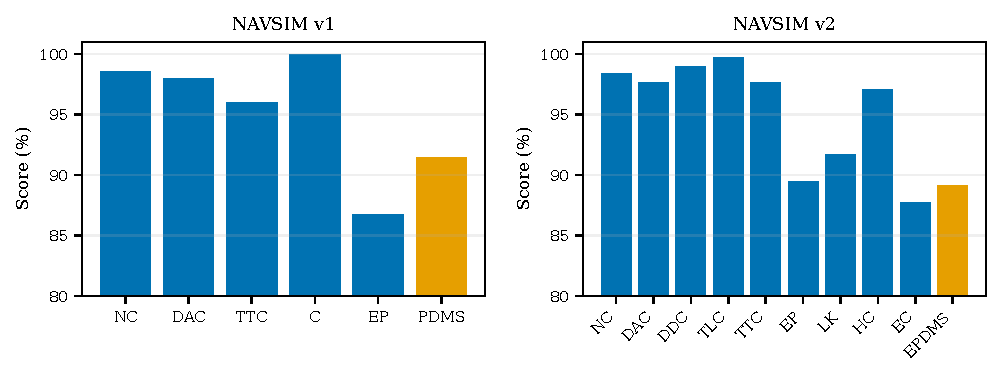
\includegraphics[width=0.76\textwidth]{figures/generated/ampt_metric_profiles.pdf}
  \caption{Scene-level reproduced AMPT component profiles on NAVSIM v1 and
  v2.  All metrics are percentages and higher is better; aggregate PDMS/EPDMS
  is shown in orange.  The profiles use 12,138 and 12,146 scored scenes,
  respectively, from one inference realization.}
  \label{fig:metric-profiles}
\end{figure*}

\paragraph{Single-trajectory inference.}
For each scene and inference seed, the model receives one observation, runs one
five-step denoising chain, and submits its single final $8\times3$ trajectory.
There is no test-time group sampling, evaluator call, candidate scoring,
reference lookup, model ensemble, or reranking.  The v1 submission provenance
independently records candidate count one, so this is a scene-level reproduced
property rather than only a methodological statement.

\paragraph{Runs and uncertainty.}
The archived v1/v2 headline exports each establish a scene-level mean for one
policy realization; they do not establish across-seed variance.  We therefore
do not attach a fabricated standard deviation to the 0.1--0.3 point increments
in the paper.  For the proposed rerun, each of seeds
20260726/20260727/20260728 produces a
complete scene export.  We first compute the mean for each run and report the
mean $\pm$ standard deviation across the three runs.  Method differences use
10,000 paired bootstrap resamples of shared scenes (resampling seeds and then
scenes within seed when multiple seeds are present), with a fixed analysis seed
of 2027 and a two-sided 95\% interval.  Recovery proportions use Wilson 95\%
intervals.  Scene bootstrap intervals from one model run describe variation
over the evaluated scenes and are explicitly not interpreted as training-seed
stability.

\paragraph{Model selection disclosure.}
The archived final v1 provenance states that \texttt{navtest} participated in
checkpoint selection.  We therefore describe the headline table as a
paper-reported benchmark comparison, not as a clean held-out model-selection
study.  The proposed rerun selects checkpoints only on the training/validation
partition, seals a checkpoint hash before \texttt{navtest}, and evaluates each
sealed hash once per inference seed.  This disclosure does not change a main
paper number; it narrows the fairness claim to what the available provenance
supports.

\subsection{The Fixed 658-Scene Recovery Protocol}
\label{sec:hard658-protocol}

The hard population is fixed before comparing optimization methods.  A scene
enters the set when the ReCogDrive IL policy receives PDMS zero in all five
sampling attempts because of collision, drivable-area violation, or both.
The resulting intersection contains 658 scene IDs.  A method \emph{recovers} a
scene when its single submitted trajectory has PDMS strictly greater than
zero under the same evaluator; the threshold is not retuned per method.

For consistency with the main paper, every supplementary hard-set analysis
uses the same archived scalar-GRPO versus historical Core-Pareto recovery pair that produced
367 and 440 positive-score scenes.  It does not substitute a later
full-benchmark checkpoint.  On the 658 fixed scenes, scalar GRPO has 367
positive and 291 zero-score outcomes, whereas the manuscript recovery
checkpoint has 440 positive and 218 zero-score outcomes.  Their paired
transition counts are 347 retained successes, 20 new failures, 93 repaired
failures, and 198 persistent failures.  Hence the net recovery is
$93-20=73$ scenes, exactly the change $440-367$, rather than a gain obtained by
hiding newly failed scenes.  The corresponding recovery rates are 55.8\%
(Wilson 95\% CI 52.0--59.5; $n=658$) and 66.9\% (63.2--70.4; $n=658$).  A
10,000-sample paired scene bootstrap gives an absolute difference of 11.1
percentage points with a 95\% interval of 8.1--14.3 points.
These intervals describe one archived checkpoint pair; no training-seed
identifier was retained for this hard-set export.

The fixed-set construction contains 480 DAC-only, 165 collision-only, and 13
joint collision-and-DAC cases according to the archived cause manifest.  The
same IDs and failure labels are used in all hard-set transition and case-table
analyses.  In particular, ``440 recovered'' means 440 positive outcomes on the
fixed original population; the transition table is required whenever the
claim is interpreted as a policy-to-policy improvement.

\subsection{Baseline and Controlled-Comparison Protocol}
\label{sec:baseline-protocol}

\begin{table*}[t]
\centering
\small
\caption{Fair-comparison protocol for main-paper baselines. All methods use one inference candidate and no test-time scorer in the paper table; unreported backbone/sensor/data details are not inferred. Result identity distinguishes reported from reproduced.}
\label{tab:baseline_protocol}
\resizebox{\textwidth}{!}{%
\begin{tabular}{lcccccc}
\toprule
method & backbone & sensors & training\_data & inference\_candidates & test\_time\_scorer & result\_identity \\
\midrule
AMPT & InternVL3-2B + ReCogDrive diffusion planner & multi-view in paper; one audited APR command resolves single camera & NAVSIM plus offline candidate/teacher pools & 1 & no & locally reproduced v1/v2 final rows; camera-manifest discrepancy disclosed \\
ReCogDrive & not disclosed in current PDF & not disclosed in current PDF & not disclosed in current PDF & 1 & no & paper reported \\
DiffusionDriveV2 & not disclosed in current PDF & not disclosed in current PDF & not disclosed in current PDF & 1 & no & paper reported \\
Drive-JEPA & not disclosed in current PDF & not disclosed in current PDF & not disclosed in current PDF & 1 & no & paper reported \\
\bottomrule
\end{tabular}%
}
\end{table*}


AMPT's v1 and v2 rows are locally reproduced from scene-level outputs.  Other
headline baseline rows are values reported in the main paper and their cited
sources; no local checkpoint, common prediction export, or common seed manifest
was found for them.  They are consequently labeled \emph{reported}, not
\emph{reproduced}.  The table records backbone, sensor interface, training
data, number of inference candidates, and use of a test-time scorer whenever
the cited evidence establishes those fields.  An unavailable field is marked
``not established by the audited source'' rather than filled by analogy with
AMPT.

For the GT/Score/Pareto/PC-MTS comparison, the paper reports a shared
initialization, diffusion SFT loss, optimizer, epoch budget, scalar-GRPO
configuration, and evaluation protocol.  The controlled reproduction
additionally seals the candidate-source manifest, fixes the proposed non-GT
sampling probability, matches the accepted candidate count, draws one target
per scene-update, and uses the same three proposed training seeds.  For Scalar GRPO versus FF-PGRPO, all rollout
chains are generated from the same initialization and sampled with the same
seed before the credit function is changed.  For No APR versus Full APR, total
optimizer steps are matched by continuing the no-APR policy with retention
targets.  These are proposed control procedures until their launch manifests
and outputs exist; the main-paper point estimates remain labeled
paper-reported.

\subsection{Reproduction and Integrity Checks}
\label{sec:reproduction-checks}

The canonical dataset stores normalized scores, benchmark and split, method,
stage, variant, round, scene ID, seed when recorded, feasibility/failure
transitions, teacher status, and its source-file/key provenance.  Validation
checks expected scene counts, duplicate scene-method records, score ranges,
the benchmark aggregate formulas, paired scene sets, and failure-state logic.
Final tables and figures are generated from that dataset; a validation failure
stops manuscript generation.  The build manifest records the command, analysis
seed, package versions, Git revision, and SHA-256 hashes of inputs and outputs.
All raw result directories are read-only, and all derived files remain under
the supplementary directory.

  \section{PC-MTS Analyses: Supervision--Optimization Alignment}
\label{sec:pcmts-analysis}

This section is needed because the quality of a supervision target and its
value for subsequent policy optimization are different quantities.  PC-MTS is
designed for the latter: it keeps a target only when its score, component-wise
trade-off, local feasibility, and proximity to the frozen learner's rollout
support are jointly acceptable.  We first examine the observed
imitation-to-optimization reversal, and then specify the controls required to
separate policy compatibility from candidate count and training budget.

\subsection{The observed supervision--optimization reversal}
\label{sec:pcmts-mismatch}

Table~\ref{tab:supervision_mismatch} restates the reported comparison from the
main paper and makes the change induced by the common scalar-GRPO stage
explicit.  Score and Pareto selection produce the two strongest imitation
checkpoints (87.2 and 87.5 PDMS), yet both deteriorate under the subsequent
optimizer.  In contrast, PC-MTS deliberately gives up 0.3--0.6 imitation
points relative to those selectors and improves by 4.2 points after the same
optimization stage.  GT supervision also improves, but finishes 0.8 points
below PC-MTS.  Thus, ranking target sets by imitation PDMS would select Pareto,
whereas ranking them by optimized PDMS selects PC-MTS.  This reversal is the
direct evidence for the mismatch claimed in the paper.

\begin{table}[t]
\centering
\small
\caption{Supervision--optimization comparison on NAVSIM v1 under single-trajectory inference. All four rows are one paper-reported run; higher PDMS and GRPO change are better, and no variance is implied.}
\label{tab:supervision_mismatch}
\resizebox{\linewidth}{!}{%
\begin{tabular}{lccccc}
\toprule
method & il\_pdms & post\_scalar\_grpo\_pdms & grpo\_change\_points & evidence & runs \\
\midrule
GT & 86.4 & 90.3 & 3.9 & paper reported & 1 reported \\
Score & 87.2 & 85.8 & -1.4 & paper reported & 1 reported \\
Pareto & 87.5 & 86.7 & -0.8 & paper reported & 1 reported \\
PC-MTS & 86.9 & 91.1 & 4.2 & paper reported & 1 reported \\
\bottomrule
\end{tabular}%
}
\end{table}


\begin{figure}[t]
  \centering
  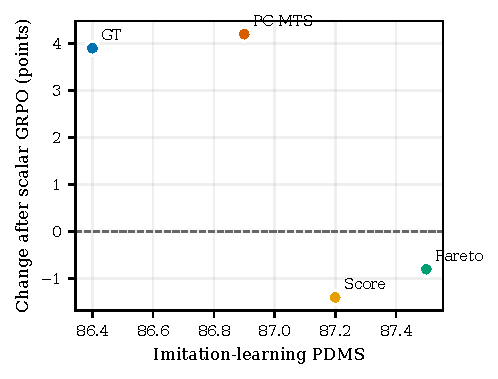
\includegraphics[width=\linewidth]{figures/generated/supervision_mismatch.pdf}
  \caption{Paper-reported imitation PDMS versus the change after the common
  scalar-GRPO stage on NAVSIM v1.  A high imitation score alone does not
  predict optimization value: Score and Pareto regress, whereas PC-MTS gains
  4.2 points.  Each marker is one reported point estimate; the paper does not
  state run/seed aggregation and no synthetic error bars are shown.}
  \label{fig:supervision-mismatch}
\end{figure}

The comparison should be interpreted at the level supported by the evidence.
It demonstrates that a higher-scoring imitation checkpoint need not be a
better starting distribution for GRPO, and that the PC-MTS set is compatible
with a large positive update in this run.  The archived paper table does not
contain scene-level outputs, acceptance counts, or multiple seeds for these
four cells.  Consequently, it does not by itself establish that the reversal
is invariant to seed, nor does it isolate candidate count from the four
filtering decisions.  We therefore do not attach synthetic error bars or
policy-distance values to these points.

\subsection{Candidate-count-matched reconstruction protocol}
\label{sec:pcmts-matched-protocol}

The released reproduction configuration turns the missing causal controls
into a predeclared, low-ambiguity experiment.  All four variants start from the
same GT-only checkpoint, use the same candidate sources, contribute exactly
one target per scene and update, train imitation learning for 200 epochs, and
then run scalar GRPO with 16 rollouts per scene for 10 epochs.  Within each
navigation-command/source stratum, accepted candidates are deterministically
subsampled to the smallest retained count across variants.  The non-GT
sampling probability is held fixed, so a method cannot receive more gradient
updates merely because it retains more candidates.  Empty strata fall back to
the logged trajectory.  In addition to final PDMS, a 300-update diagnostic
records the early GRPO gain before long-horizon training effects can dominate.

For a fully specified reconstruction when the original resolved PC-MTS
manifest is unavailable, the release marks the following as \emph{proposed
reproduction settings}, not measured settings of the reported run: a rollout
bank of 16, $K=3$ neighbors, a command-conditional 0.95 calibration quantile,
and eight temporally correlated local perturbations.  The rollout bank and
calibration queries are disjoint by construction.  Three predeclared training
seeds (20260726, 20260727, and 20260728) are used for the reconstruction, while
bootstrap seed 2027 is reserved for analysis and is never treated as an additional
training run.  These choices fill the executable configuration without
retroactively attributing unrecorded hyperparameters to the main-paper result.

For each run, the pipeline records retained candidates, acceptance rate,
candidate-source composition, feasible rollout rate, feasible high-quality
rate, all-infeasible-group rate, zero-score rate, the 10th percentile,
CVaR-10, 300-update gain, and final scalar-GRPO PDMS.  Method differences are
computed on identical scenes with a 10,000-resample paired bootstrap; means
and standard deviations are reported across the three training seeds.

\subsection{Filter attribution and sensitivity}
\label{sec:pcmts-components}

The component experiment is cumulative: (i) aggregate Score only, (ii) Score
plus the component-wise Pareto gate, (iii) the preceding gates plus calibrated
policy compatibility, and (iv) the full selector with local-feasibility
testing.  Counts are matched after each gate, rather than relaxing a stricter
gate to reach a target count.  This distinction matters: a matched count must
not reintroduce candidates that failed the mechanism being tested.  The
decisive diagnostic is not imitation PDMS alone, but whether adding a gate
raises feasible rollout density and converts the fixed-budget GRPO change from
negative to positive.

The companion sensitivity protocol varies one factor at a time: rollout-bank
size in $\{8,16,32\}$, $K$ in $\{1,3,5\}$, calibration quantile in
$\{0.90,0.95,0.975\}$, and perturbation count in $\{4,8,16\}$.  Compatibility
alternatives are compared at the same acceptance rate: candidate-to-GT
ADE/FDE, distance to the deterministic policy output, minimum rollout-bank
distance, average $K$-nearest distance, and command-calibrated $K$-nearest
distance.  These are evidence-bounded planned analyses: the release contains
their configurations and logging schema, but no unexecuted outcome is used to
support the paper's reported 91.1 PDMS.

Taken together, the existing reversal and the matched protocol close two
different parts of the argument.  The former establishes that isolated target
quality can disagree with downstream optimization value; the latter defines
the experiment needed to attribute that disagreement specifically to policy
compatibility rather than supervision quantity.

  \section{FF-PGRPO Analyses: Feasibility Before Positive Credit}
\label{sec:ffpgrpo-analysis}

Aggregate reward can hide an unsafe trade: progress or comfort may increase
enough to give positive standardized advantage even when collision avoidance,
drivable-area compliance, or a protected reference metric regresses.  The
purpose of FF-PGRPO is therefore not merely to reshape the scalar score, but to
change which rollouts are eligible for positive credit.

\subsection{What the stage ablation establishes}
\label{sec:ffpgrpo-stage-ablation}

On NAVSIM v1, the no-stage baseline in the main ablation has 86.5 PDMS, 98.1
NC, 94.7 DAC, 94.2 TTC, and 80.9 EP.  Applying FF-PGRPO without PC-MTS reaches
91.0 PDMS, with 98.4 NC, 98.0 DAC, 95.8 TTC, and 85.93 EP.  With PC-MTS as the
initialization, FF-PGRPO reaches 91.1 PDMS, 98.5 NC, 98.0 DAC, 96.0 TTC, and
86.0 EP before APR.  The improvement is therefore not produced by sacrificing
the displayed hard-safety components for progress: DAC improves by 3.3 points
and TTC by 1.6 points in the FF-PGRPO-only row, while EP increases by 5.03
points.  These are paper-reported point estimates whose run/seed aggregation
is not stated, so the small 0.1-point
difference between the two FF-PGRPO rows is not presented as a stable gain.

\begin{table*}[t]
\centering
\small
\caption{Stage-wise NAVSIM v1 ablation under single-trajectory inference. Higher is better. Rows are one paper-reported run; only the final AMPT row is independently reproduced from 12,138 scene scores.}
\label{tab:stage_ablation}
\resizebox{\textwidth}{!}{%
\begin{tabular}{lcccccccccccc}
\toprule
configuration & pcmts & scalar\_grpo & ff\_pgrpo & apr & NC & DAC & TTC & C & EP & PDMS & evidence & runs \\
\midrule
GT-only & no & no & no & no & 98.1 & 94.7 & 94.2 & 100.0 & 80.9 & 86.5 & paper reported & 1 reported \\
PC-MTS & yes & no & no & no & 98.2 & 95.2 & 94.5 & 100.0 & 81.3 & 86.9 & paper reported & 1 reported \\
Scalar optimization & no & yes & no & no & 98.4 & 98.0 & 95.8 & 100.0 & 85.93 & 91.0 & paper reported & 1 reported \\
PC-MTS + FF-PGRPO & yes & no & yes & no & 98.5 & 98.0 & 96.0 & 100.0 & 86.0 & 91.1 & paper reported & 1 reported \\
Full AMPT & yes & no & yes & yes & 98.5 & 98.0 & 96.0 & 100.0 & 86.7 & 91.4 & paper reported / final row scene-reproduced & 1 reported + 12138 scenes final \\
\bottomrule
\end{tabular}%
}
\end{table*}


This result is consistent with the proposed ordering---recover feasibility,
then optimize continuous quality---but an aggregate stage ablation cannot
directly reveal the sign of individual rollout credits.  The fixed hard-scene
transition in Section~\ref{sec:hard658} provides scene-level evidence, and the
instrumentation below defines the rollout-level test.

\subsection{Credit diagnostics}
\label{sec:ffpgrpo-credit-diagnostics}

For rollout $i$, let $A_i>0$ denote positive assigned advantage and let
$V_i=1$ denote a violation of any hard-feasibility, protected-reference, or
admissible-Pareto condition.  We report
\begin{equation}
  \mathrm{PCVR} =
  \frac{\sum_i \mathbb{1}[A_i>0]V_i}
       {\sum_i \mathbb{1}[A_i>0]},
  \label{eq:positive-credit-violation}
\end{equation}
and separately count reference-regressing and Pareto-dominated positive
credits.  A denominator of zero is reported as ``no positive credits,'' not as
zero violation.  FF-PGRPO's implementation makes a violating rollout
ineligible for positive credit and exposes assertions for this contract.  The
archived training run, however, does not contain the per-rollout trace needed
to quote an observed PCVR; we do not convert a code invariant into a fabricated
measured rate.

The stepwise mechanism ablation adds: (i) the hard feasibility gate, (ii) the
coherent-reference guard, (iii) the Pareto positive-credit gate, and (iv) the
all-infeasible recovery rule.  Every variant logs group state
(all-feasible/mixed/all-infeasible), feasibility rate, positive and negative
advantage means, PCVR, reference-regressing positive-credit rate,
dominated-positive-credit rate, zero-to-feasible repair, positive-to-zero
regression, and updates until the first feasible rollout.  The coherent
reference is always one executable trajectory.  The historical
component-wise envelope remains only as an ablation because combining the best
value of each metric from different trajectories may describe no realizable
plan and can make every sampled rollout appear to regress.

The low-cost diagnostic run uses the paper's group size of 16 and stops at 300
updates; the final run uses the reported 10 epochs.  All variants share the
same sampled rollout tensors when credit is recomputed offline, which makes
the initial credit-assignment comparison independent of policy drift.  New
training is required only for the subsequent learning curves and remains
disabled unless explicitly enabled.

\subsection{Hard-scene evidence for feasibility-first recovery}
\label{sec:ffpgrpo-hard-evidence}

The manuscript recovery checkpoint is evaluated on the same 658-scene set as
scalar GRPO.  Scalar GRPO produces a positive score in 367 scenes (55.8\%,
95\% Wilson CI 52.0--59.5\%), whereas the AMPT recovery checkpoint is positive
in 440 scenes (66.9\%, CI 63.2--70.4\%).  The comparison uses a single
trajectory per scene and neither method uses test-time sampling, scoring, or
reranking.  Crucially, the paired transition is not merely a difference of
gross counts: 93 scalar-GRPO zeros become positive, 20 scalar-GRPO positives
become zero, 347 successes are retained, and 198 failures persist.  Net
recovery is therefore $93-20=73$ scenes, or 11.1 percentage points.  A
10,000-resample scene-paired bootstrap (analysis seed 2027) gives a 95\% CI of
8.1--14.3 percentage points for this paired change.  This interval quantifies
scene variation for this fixed checkpoint pair; it does not replace missing
multi-seed training uncertainty.

The subset mean PDMS increases from 0.5101 to 0.6145.  The corresponding
component means change from 0.8381 to 0.8815 for NC, 0.7052 to 0.7781 for DAC,
0.7705 to 0.8161 for TTC, and 0.4956 to 0.5932 for EP; comfort increases from
0.9985 to 1.0000, while DDC changes from 0.9567 to 0.9521.  This last decrease
is why protected metrics must be reported next to aggregate recovery rather
than summarized as universal component-wise improvement.  The complete
transition and failure-type decomposition are given in
Section~\ref{sec:hard658}.

The aggregate ablation, paired hard-scene transition, and positive-credit
instrumentation serve complementary roles.  The first shows the overall stage
gain, the second verifies that recovery is net positive rather than purchased
entirely with new failures, and the third is the predeclared test of the
claimed credit-assignment mechanism.

  \section{APR Analyses: Dynamic, Policy-Relative Teachers}
\label{sec:apr-analysis}

APR addresses a moving-target problem.  A trajectory that is a useful local
teacher for the current policy can become redundant after refinement, while a
previously distant candidate can enter the policy's compatible neighborhood.
The relevant question is therefore not whether additional optimization steps
help, but whether rebuilding and re-auditing the teacher set provides useful
targets while retaining already safe behavior.

\subsection{Round-wise behavior and protected components}
\label{sec:apr-rounds}

The main paper reports a monotonic sequence of 91.10, 91.21, 91.37, and 91.45
PDMS from Round 0 through Round 3, corresponding to gains of $+0.11$, $+0.16$,
and $+0.08$.  In the stage ablation, adding APR to the PC-MTS+FF-PGRPO policy
raises PDMS from 91.1 to 91.4 and EP from 86.0 to 86.7, while the displayed NC,
DAC, TTC, and comfort values remain 98.5, 98.0, 96.0, and 100, respectively.
This pattern is aligned with APR's design: local teacher updates increase
progress without visible regression in the protected components at the
reported precision.

Each round value is a reported checkpoint summary; its run/seed aggregation is
not stated.  No across-seed
standard deviation is available, and the 0.08--0.16 point increments are not
claimed to be independently significant.  Moreover, the archived experiment
history contains accepted and rejected branches rather than a single complete
three-round hash chain; the four values above are therefore treated as the
paper's round-level summary, not as permission to infer missing intermediate
measurements.

\begin{table}[t]
\centering
\small
\caption{Paper-reported NAVSIM v1 APR progression under single-trajectory inference. Higher is better. Run/seed aggregation is not stated and no training-seed confidence interval is available.}
\label{tab:apr_rounds}
\resizebox{\linewidth}{!}{%
\begin{tabular}{lcccc}
\toprule
round & pdms & gain\_points & evidence & runs \\
\midrule
0 & 91.1 & 0.0 & paper reported & reported point; run/seed aggregation not stated \\
1 & 91.21 & 0.11 & paper reported & reported point; run/seed aggregation not stated \\
2 & 91.37 & 0.16 & paper reported & reported point; run/seed aggregation not stated \\
3 & 91.45 & 0.08 & paper reported / final score scene-reproduced & reported point + 12138 final scenes; run aggregation not stated \\
\bottomrule
\end{tabular}%
}
\end{table}


\begin{figure}[t]
  \centering
  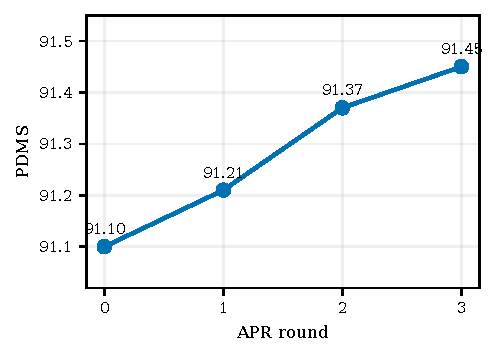
\includegraphics[width=\linewidth]{figures/generated/apr_rounds.pdf}
  \caption{Paper-reported NAVSIM v1 progression across APR rounds.  The final
  point is reproduced at scene level, but the small round increments are from
  one reported sequence and carry no across-seed error bar.}
  \label{fig:apr-rounds}
\end{figure}

\subsection{Teacher audit and post-interpolation evaluation}
\label{sec:apr-teacher-audit}

One traceable APR teacher-construction pass starts from 39,261 strict external
trajectories: 25,402 (64.7\%) from one driving-policy source and 13,859
(35.3\%) from a second source.  After interpolation with coefficient 0.25 and
exact re-evaluation, 28,910 targets remain, an acceptance rate of 73.6\%; the
remaining 10,351 are rejected.  These counts are from one audited navtrain
construction pass and are not presented as the source proportions of every
APR round.  They nevertheless establish an important operational fact:
interpolation is followed by evaluator-based admission, and the check is
non-vacuous---more than one quarter of the pre-audit union does not enter the
distillation set.

\begin{table}[t]
\centering
\small
\caption{Audited APR teacher-pool construction on NAVSIM navtrain. Counts are from one archived teacher audit; the 28,910 accepted teachers follow interpolation and exact re-evaluation. Higher acceptance is not inherently better because guards constrain quality.}
\label{tab:apr_teacher_pool}
\resizebox{\linewidth}{!}{%
\begin{tabular}{lcccc}
\toprule
step & source & count & acceptance\_definition & evidence \\
\midrule
source selection & DriVor & 25402 & source-specific strict candidates & archived APR runbook \\
source selection & DiffusionDriveV2 & 13859 & source-specific strict candidates & archived APR runbook \\
strict union & merged sources & 39261 & feasible and component-protected before interpolation & deterministic sum of audited source counts \\
post-interpolation audit & accepted teachers & 28910 & alpha 0.25 then exact re-evaluation & archived APR runbook \\
\bottomrule
\end{tabular}%
}
\end{table}


Teacher status is defined relative to the current policy.  A candidate is
\emph{accepted} when its evaluated local target is feasible, exceeds the
current single prediction by the required margin, preserves protected
metrics, and stays inside the current rollout neighborhood.  An accepted
teacher becomes \emph{expired} if it fails those tests after the policy is
updated.  A previously rejected candidate is \emph{newly activated} if it
passes after the rollout bank and current prediction are regenerated.  These
definitions prevent lifecycle counts from being conflated with raw pool size.

The interpolation search is descending: larger moves are evaluated first and
the first admissible move is retained.  Every accepted target stores the
teacher, current prediction, interpolation coefficient, post-interpolation
score, protected-metric deltas, compatibility distance, and evaluator hash.
No-interpolation and no-post-evaluation controls remove different safeguards:
the former jumps directly to the teacher, whereas the latter retains a local
trajectory without verifying that interpolation preserved feasibility.

\subsection{Step-matched controls}
\label{sec:apr-controls}

The release defines eight variants from the same Round-0 checkpoint and
matches the total number of optimizer updates: extra training on the existing
mixture, one-shot distillation, repeated use of a fixed teacher set, dynamic
teachers, dynamic teachers without interpolation, without post-interpolation
re-evaluation, without policy retention, and full APR.  The dynamic-teacher
and full-APR variants rebuild predictions, rollout banks, and teacher audits at
the same three round boundaries reported in the paper.  The fixed-teacher
variant repeats the Round-1 set without re-ranking it; the extra-training
control receives the same update count but no new teacher target.  This design
separates four possible explanations: more updates, teacher supervision in
general, teacher-set rebuilding, and the interpolation/retention safeguards.

For every round, the required report contains PDMS and all components,
regressed scenes, new failures, accepted/expired/newly activated teachers,
mean and median verified teacher advantage, interpolation-coefficient
distribution, and scene coverage.  A checkpoint is promoted only if its
single-trajectory aggregate score improves and protected metrics pass the
same non-regression audit; otherwise the previous checkpoint remains the
dynamic anchor.  Training ends after three promoted rounds or when no audited
local target remains.  These controls are configured but not represented as
measured results in this supplement, because running them would require new
training.

Optional task-vector consolidation is kept separate from teacher discovery.
The implementation can mask low-salience coordinates, require directional
agreement, bound each branch norm and the total displacement from the current
anchor, and then evaluate the merged checkpoint.  The best-branch, simple
average, task-arithmetic, and TIES-style controls are required before assigning
an independent gain to merging~\cite{taskarithmetic2023,ties2023}.  In the
absence of a stable, step-matched gain, merging should be read as a conservative
checkpoint-consolidation detail, not as the source of APR's teacher lifecycle.

The present evidence therefore supports two bounded statements: the reported
APR rounds are monotonic and preserve the displayed safety/compliance metrics,
and an audited construction pass materially filters proposed local targets
after re-evaluation.  The step-matched variants above are the necessary test
for the stronger causal claim that dynamic rebuilding, rather than additional
training alone, explains the full increment.

\begin{table}[t]
\centering
\small
\caption{APR fixed-teacher diagnostic on NAVSIM v1. The archived fixed-set continuation decreases from its 91.2766 anchor, whereas the 91.45 endpoint is the paper's compressed dynamic-round report; the rows are diagnostic rather than a step-matched causal ablation.}
\label{tab:apr_fixed_teacher}
\resizebox{\linewidth}{!}{%
\begin{tabular}{lccc}
\toprule
policy\_or\_epoch & pdms & interpretation & evidence \\
\midrule
dynamic-teacher anchor & 91.2766 & accepted dynamic-teacher checkpoint & archived APR runbook \\
fixed-set continuation epoch 0 & 91.2526 & below dynamic-teacher anchor & archived APR runbook \\
fixed-set continuation epoch 1 & 91.2311 & further below dynamic-teacher anchor & archived APR runbook \\
paper APR round 3 & 91.45 & compressed round-level paper report & paper reported \\
\bottomrule
\end{tabular}%
}
\end{table}


  \section{Failure Recovery and Qualitative Diagnostics}
\label{sec:failure-qualitative}

Qualitative evidence is most useful when organized by a mechanism and tied to
scene-level metrics.  We therefore analyze the fixed hard set first, then give
traceable examples of recovered, persistent, and newly introduced failures.
All quantitative hard-set results and the mechanism-organized case table use
the same historical checkpoint pair as the main paper's 367-versus-440
recovery claim.  The final full-benchmark visualization is separately labeled
and is not used in the 658-scene recovery analysis.

\subsection{Construction of the fixed 658-scene set}
\label{sec:hard658}

The set contains 658 NAVSIM v1 scenes for which the initial ReCogDrive policy
obtained exactly zero PDMS in all five construction samples because of an
at-fault collision (NC), drivable-area violation (DAC), or both.  The set is
fixed before comparing the scalar-GRPO and AMPT recovery checkpoints.  Under
single-trajectory evaluation, scalar GRPO is positive on 367 and zero on 291
scenes; the AMPT recovery checkpoint is positive on 440 and zero on 218.

The paired $2\times2$ transition is
\begin{equation}
\begin{array}{c|cc|c}
 & \multicolumn{2}{c|}{\text{AMPT recovery checkpoint}} & \\
\text{scalar GRPO} & \text{zero} & \text{positive} & \text{row total} \\
\hline
\text{zero}     & 198 & 93  & 291 \\
\text{positive} & 20  & 347 & 367 \\
\hline
\text{column total} & 218 & 440 & 658
\end{array}.
\label{eq:hard658-transition}
\end{equation}
Hence 93 failures are repaired, 347 successes are retained, 198 failures
persist, and 20 new failures appear.  The net change is $93-20=73$, exactly the
difference between the gross positive counts $440-367$.  This distinction is
important: 440/658 is the gross recovery rate relative to the policy used to
construct the hard set, whereas 93 and 20 describe the paired transition from
scalar GRPO to the AMPT recovery checkpoint.  The resulting 11.1-percentage-
point paired improvement has a scene-bootstrap 95\% CI of 8.1--14.3 points
(10,000 resamples, seed 2027).  It is a net improvement rather than an exchange
of an equal number of old and new failures.

\begin{table}[t]
\centering
\small
\caption{Recovery on the same 658 NAVSIM v1 scenes under one archived comparison. Rates use Wilson 95\% intervals over scenes; this interval does not represent training-seed uncertainty. Higher recovery is better.}
\label{tab:failure_recovery}
\resizebox{\linewidth}{!}{%
\begin{tabular}{lcccccc}
\toprule
Method & Positive & Zero & Recovery rate (\%) & Wilson 95\% CI (\%) & Runs & Scenes \\
\midrule
Scalar GRPO & 367 & 291 & 55.8 & [52.0, 59.5] & 1 archived comparison & 658 \\
AMPT recovery checkpoint & 440 & 218 & 66.9 & [63.2, 70.4] & 1 archived comparison & 658 \\
\bottomrule
\end{tabular}%
}
\end{table}

\begin{table}[t]
\centering
\small
\caption{Paired recovery change on 658 NAVSIM v1 scenes. The 11.1-point gain has a scene-paired bootstrap interval (10,000 resamples, analysis seed 2027); higher net repair is better. One archived model pair is available.}
\label{tab:failure_net_gain}
\resizebox{\linewidth}{!}{%
\begin{tabular}{lcccccc}
\toprule
Absolute gain (pp) & Paired 95\% CI (pp) & Zero-to-positive & Positive-to-zero & Net repair & Scenes & Runs \\
\midrule
11.1 & [8.1, 14.3] & 93 & 20 & 73 & 658 & 1 archived comparison \\
\bottomrule
\end{tabular}%
}
\end{table}


\begin{figure}[t]
  \centering
  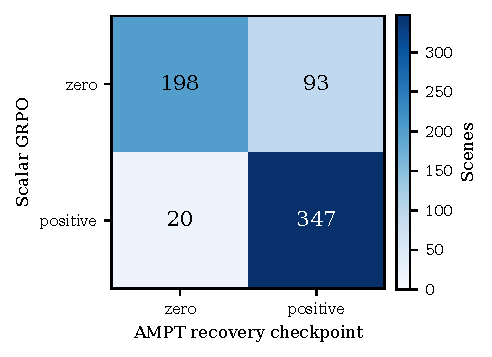
\includegraphics[width=\linewidth]{figures/generated/failure_transition.pdf}
  \caption{Scalar-GRPO to AMPT transition on the fixed 658-scene set.  The
  off-diagonal cells expose both 93 repairs and 20 regressions, rather than
  reporting gross recovery alone.}
  \label{fig:failure-transition}
\end{figure}

The original hard-set taxonomy contains 480 DAC-only scenes, 165 collision-
only scenes, 13 scenes failing both, and no residual ``other'' category.  The
paired repairs/new failures are 59/14 for DAC-only, 32/6 for collision-only,
and 2/0 for the joint category, giving net changes of 45, 26, and 2 scenes.
The gains are therefore not concentrated in only one failure type, although
the small joint category is descriptive rather than statistically decisive.

\begin{table}[t]
\centering
\small
\caption{Failure-type decomposition for the fixed 658 NAVSIM v1 scenes. Repairs and regressions use the scalar-GRPO to AMPT transition; net repairs sum to 73. One archived comparison; higher net repair is better.}
\label{tab:failure_causes}
\resizebox{\linewidth}{!}{%
\begin{tabular}{lcccc}
\toprule
Failure type & Scenes & Repairs & Regressions & Net repair \\
\midrule
DAC-only/all-fail & 480 & 59 & 14 & 45 \\
collision-only/all-fail & 165 & 32 & 6 & 26 \\
collision + DAC & 13 & 2 & 0 & 2 \\
\bottomrule
\end{tabular}%
}
\end{table}


\begin{figure}[t]
  \centering
  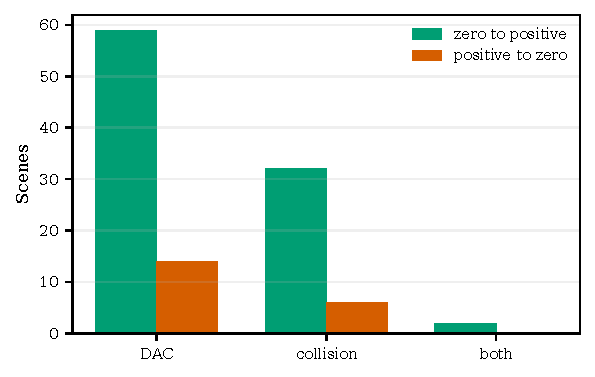
\includegraphics[width=\linewidth]{figures/generated/failure_cause_recovery.pdf}
  \caption{Repairs and regressions by the fixed hard-set cause taxonomy.  The
  net changes are 45 DAC, 26 collision, and 2 joint cases, totaling 73.}
  \label{fig:failure-causes}
\end{figure}

\subsection{Traceable scene cases}
\label{sec:traceable-cases}

Table~\ref{tab:hard658-cases} selects cases by transition type, not by visual
appeal.  Navigation commands come from the corresponding NAVSIM scene
metadata; scores and components come from the fixed paired evaluation.  The
table uses full scene identifiers so every row can be regenerated.  Component
pairs are scalar-GRPO $\rightarrow$ AMPT-recovery values.

\begin{table*}[t]
\centering
\small
\caption{Mechanism-organized examples from the fixed 658-scene set. Scene IDs and PDMS values are reproduced from the archived comparison; commands are joined from audited scene metadata. These selected cases are not an unbiased benchmark sample.}
\label{tab:hard658-cases}
\resizebox{\textwidth}{!}{%
\begin{tabular}{lccccccccc}
\toprule
Scene ID & Command & Outcome & PDMS & NC & DAC & TTC & EP & DDC & Diagnosis \\
\midrule
00fcad6d092c5e8e & left & repaired & 0.000 -> 1.000 & 0.000 -> 1.000 & 1.000 -> 1.000 & 0.000 -> 1.000 & 0.000 -> 1.000 & 1.000 -> 1.000 & Collision/TTC failure repaired without protected regression. \\
03aa8a0576a25b63 & right & repaired & 0.000 -> 0.963 & 1.000 -> 1.000 & 0.000 -> 1.000 & 1.000 -> 1.000 & 0.000 -> 0.912 & 1.000 -> 1.000 & Drivable-area failure repaired while NC and TTC remain feasible. \\
1148c72f141c532d & left & partial repair & 0.000 -> 0.583 & 0.000 -> 1.000 & 0.000 -> 1.000 & 0.000 -> 0.000 & 0.000 -> 1.000 & 1.000 -> 1.000 & Both hard failures repaired; TTC remains the limiting component. \\
00016f8b45c25a1d & left & persistent & 0.000 -> 0.000 & 1.000 -> 1.000 & 0.000 -> 0.000 & 1.000 -> 1.000 & 0.000 -> 0.000 & 0.000 -> 0.000 & DAC/progress failure persists under both audited checkpoints. \\
4b4a268bee4c5ab5 & left & regressed & 1.000 -> 0.000 & 1.000 -> 1.000 & 1.000 -> 0.000 & 1.000 -> 1.000 & 1.000 -> 0.000 & 1.000 -> 1.000 & A DAC regression creates a new zero and motivates retention. \\
\bottomrule
\end{tabular}%
}
\end{table*}


The first two cases are consistent with feasibility-oriented recovery: a hard
component changes from zero to one and positive PDMS returns.  Scene-level
before/after metrics do not identify the temporal order of training updates.
The third shows why ``recovered'' does not mean component-wise perfect.  The
fourth remains a DAC/progress failure under both audited checkpoints; without a
candidate/rollout manifest, the metrics do not identify whether pool coverage,
policy support, or optimization is responsible.  The fifth prevents
survivorship bias in the qualitative analysis and
motivates APR retention; it is one of the 20 positive-to-zero transitions
already charged against net recovery.

\subsection{Mechanism-centered visualization protocol}
\label{sec:qualitative-protocol}

The supplied renderer groups panels by decision rather than by scene
similarity.  A PC-MTS panel overlays an accepted candidate, a rejected distant
candidate, the logged trajectory, and the frozen-policy rollout neighborhood.
An FF-PGRPO mixed-group panel distinguishes unsafe, feasible-but-dominated,
and admissible Pareto-positive rollouts and prints their assigned advantages;
an all-infeasible panel shows the coherent recovery reference.  An APR panel
shows the current prediction, raw teacher, evaluated interpolant, and the
accepted/expired/newly-activated lifecycle state.  Every rendered panel reads
the scene id, command, component scores, and method name from its manifest and
uses a common legend: blue for the current prediction, green for an accepted
or positively credited trajectory, orange for a dominated/expired trajectory,
red for an unsafe trajectory, and black dashed for the coherent reference.

This protocol is also a safeguard against overinterpretation.  A camera/BEV
image is emitted only when the frame, command, all trajectories, and evaluator
record share the same scene identifier.  The metric-only cases in
Table~\ref{tab:hard658-cases} remain quantitative case studies if those visual
assets are unavailable; no unrelated camera frame or hand-drawn trajectory is
substituted merely to complete a panel.

\begin{figure*}[t]
  \centering
  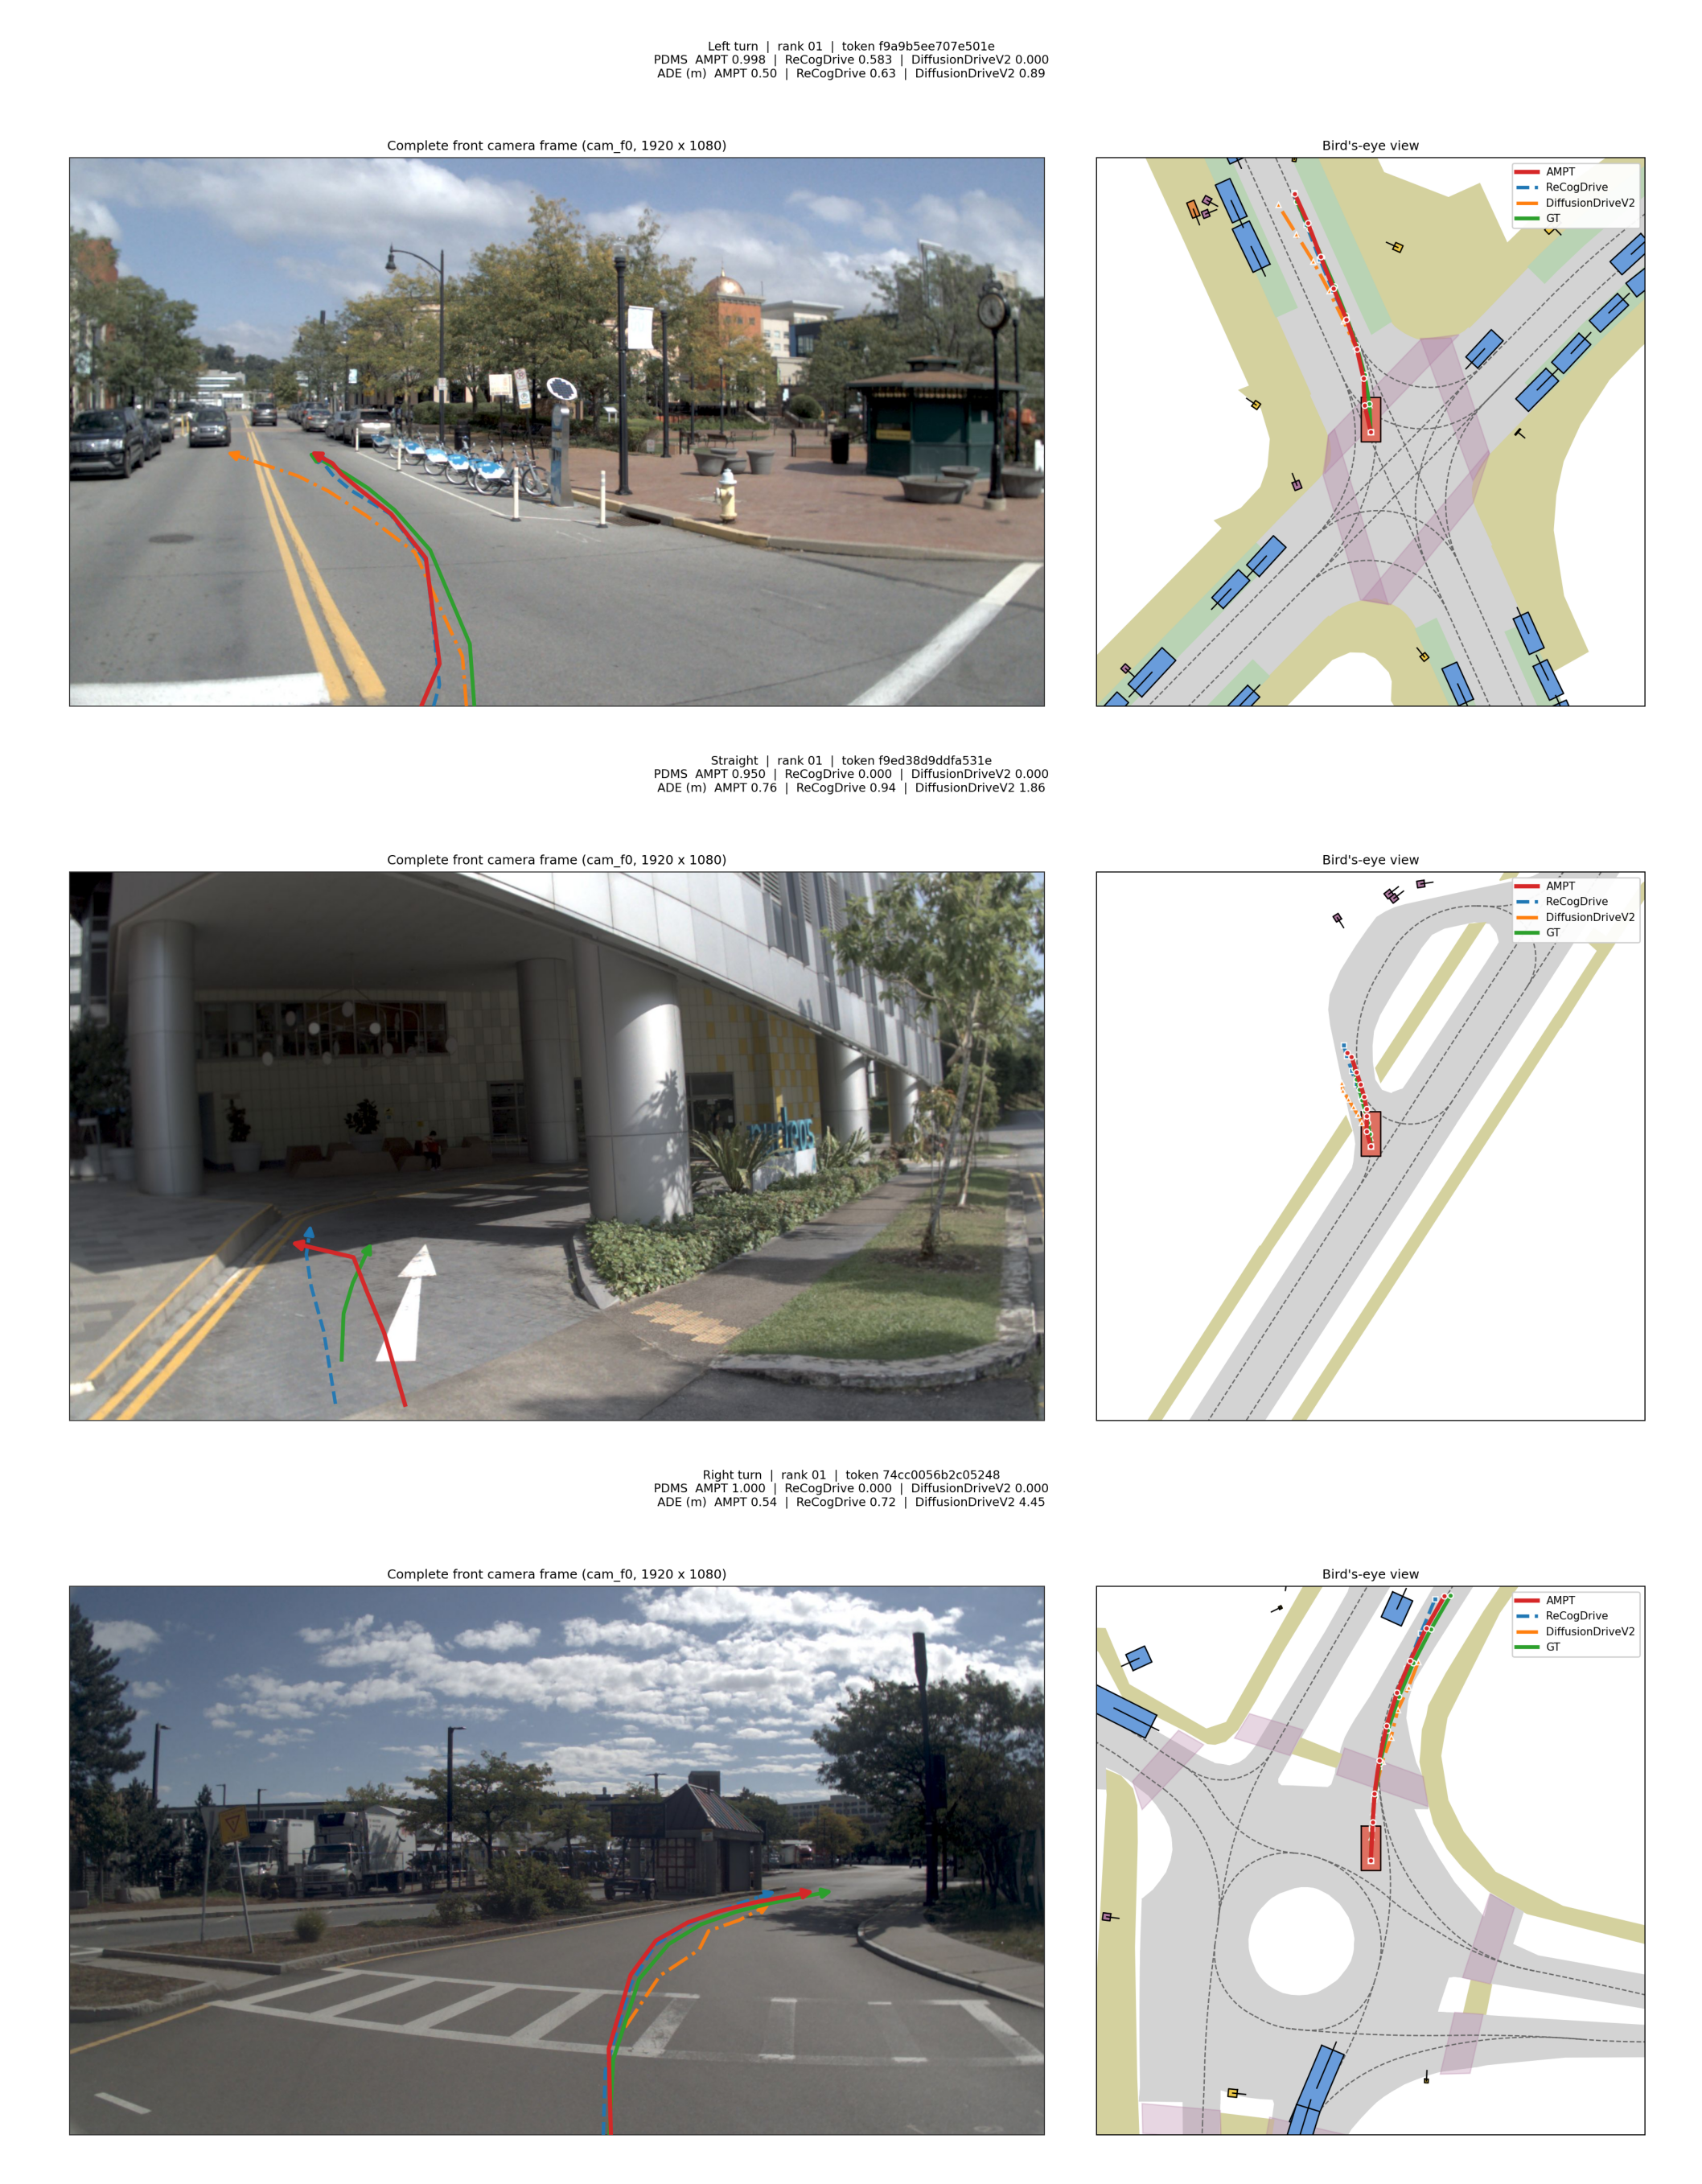
\includegraphics[width=0.92\textwidth]{figures/generated/qualitative_selected_cases.png}
  \caption{Three selected full-benchmark NAVSIM v1 cases (left, straight, and
  right commands) rendered from the separately audited final-AMPT manifest.
  Each row contains the complete front frame, bird's-eye view, scene ID,
  command, color legend, PDMS, and trajectory error.  These examples are not
  members of, and contribute no statistics to, the historical 658-scene
  recovery comparison; they illustrate final-policy behavior only.}
  \label{fig:qualitative-selected}
\end{figure*}

\clearpage

  \section{Additional Related Work, Fair Comparison, and Limitations}
\label{sec:related-limitations}

\subsection{Related perspectives}

\textbf{Support-aware policy improvement.}
Conservative offline policy-improvement methods limit updates in regions where
the behavior data provide weak support.  SPIBB constrains uncertain decisions
to the baseline policy~\cite{spibb2019}, while BEAR regularizes a learned policy
toward the behavior distribution~\cite{bear2019}.  PC-MTS shares the support
intuition but applies it before optimization: it filters trajectory-level
supervision using samples from the frozen learner, with command-conditional
calibration and a local feasibility test.  It is not a general monotonic-
improvement guarantee; its role is to avoid moving the imitation policy into a
region where downstream rollout optimization has poor local support.

\textbf{Multi-objective and Pareto optimization.}
Multi-objective reinforcement learning studies policies under vector-valued
returns and alternative preference models~\cite{roijers2013}.  AMPT does not
seek a global set of Pareto-optimal policies.  PC-MTS uses a scene-local Pareto
filter for supervision, and FF-PGRPO uses a hierarchy: hard feasibility and
coherent-reference guards are evaluated before a rollout can receive positive
Pareto credit.  This order is essential when an aggregate score can compensate
for a protected regression.

\textbf{Advantage-weighted behavior learning.}
Advantage-weighted regression turns estimated advantages into weights for
supervised policy updates~\cite{awr2021}.  APR is related at the loss level,
but its weights are attached only after a candidate is compared with the
current single-trajectory prediction, locally interpolated, and re-evaluated.
Teacher admission and policy retention are therefore as important as the
weighting function itself.

\textbf{Model merging.}
Task arithmetic combines model displacements relative to a shared
anchor~\cite{taskarithmetic2023}, and TIES resolves redundancy and sign
conflicts before merging~\cite{ties2023}.  AMPT may use an anchor-constrained
variant to consolidate APR branches, but merging is optional and is separated
from teacher selection.  Passing parameter-space norm and sign checks does not
imply behavioral safety; every merged checkpoint must still undergo the same
single-trajectory evaluator audit.

\subsection{Fair-comparison boundary}
\label{sec:fair-comparison}

AMPT uses one predicted trajectory at inference.  Policy rollout banks,
candidate pools, coherent references, group sampling, specialist policies, and
the offline evaluator are training-only; there is no test-time scorer,
best-of-$N$ selection, or candidate reranking.  This contract is present in the
paper and is independently supported by the v1 submission provenance.

The released v1 scene export contains 12,138 successfully scored scenes from
12,146 predictions; the eight unscored predictions are disclosed rather than
imputed.  The v2 export contains 12,146 successful scene scores.  Its EC
aggregation follows the official evaluator, although a direct EC value is
present for 10,040 rows.  Scene-bootstrap intervals resample these scored
scenes and are explicitly labeled as scene uncertainty; they are not a
substitute for independent training runs.

The baseline rows in the main tables are treated as \emph{reported} unless a
local scene export and matching protocol are available.  AMPT's v1/v2 rows are
reproduced from scene-level outputs, but protocol matching is not established
for every external baseline.  Moreover, the audited v1 provenance records use
of navtest for checkpoint selection.  We therefore avoid a strict held-out
state-of-the-art claim and report protocol fields---backbone, sensors, training
data, inference candidates, and test-time scoring---alongside each comparison.

The 658-scene result uses the recovery checkpoint and checkpoint pair specified
by the main-paper analysis.  It is a fixed-subset diagnostic, not a claim that
every later checkpoint must induce the same transitions.  Reporting the full
$2\times2$ matrix in Eq.~\ref{eq:hard658-transition} makes the gross and net
notions of recovery explicit.

\subsection{Limitations}
\label{sec:limitations}

\textbf{Finite support estimates.}
Compatibility is estimated from a finite rollout bank.  Sparse commands or
multi-modal scenes can make a genuinely useful target appear distant, and the
calibrated neighborhood is only as representative as the frozen policy
samples.  Increasing bank size improves coverage but raises offline inference
and storage cost.

\textbf{Evaluator bias and non-reactive evaluation.}
All three stages use an offline NAVSIM evaluator for filtering, credit, or
teacher validation.  Systematic evaluator errors can therefore be amplified
across stages.  NAVSIM's non-reactive agents also cannot reveal how other road
users would respond to the learned trajectory; feasibility under this scorer
is not a closed-loop safety guarantee.

\textbf{Candidate-pool ceiling.}
APR can select and localize only behaviors represented in its multi-source
pool.  If no source proposes a valid maneuver, rebuilding the pool changes no
target.  The persistent case in Table~\ref{tab:hard658-cases} establishes
persistence under two audited checkpoints, but cannot diagnose this pool
ceiling without a per-scene candidate manifest.

\textbf{Locality can reject long-horizon value.}
The policy-compatibility filter intentionally favors learnable local targets.
It may reject a distant behavior that is initially difficult to imitate but
would be valuable after a longer curriculum.  Policy-dependent teacher-value
and cross-policy selection experiments are therefore important follow-ups.

\textbf{Benchmark-specific hierarchy.}
The ordering of NC/DAC feasibility, DDC/TLC guards, progress floors, and
continuous Pareto objectives reflects NAVSIM metrics.  Transferring AMPT to a
new benchmark requires revalidating the hierarchy and calibration thresholds,
not merely renaming metric fields.

\textbf{No behavioral semantics for parameter merging.}
Task-vector masks, direction agreement, and norm constraints bound parameter
movement but do not provide a semantic or safety guarantee.  If its independent
gain is not stable across seeds and step-matched controls, merging should
remain an implementation detail.

\textbf{Statistical scope.}
The supervision comparison, stage ablation, and APR round table are available
as reported point estimates rather than three-seed aggregates.  Small APR
increments must not be described as stable until the configured multi-seed
controls are run.  The paired 658-scene interval establishes a robust scene-
level net transition for one checkpoint pair, but does not measure training-
seed variation.

These limitations narrow rather than alter the paper's central claim.  The
currently traceable evidence establishes the supervision--optimization
reversal, a large feasibility-oriented stage gain, monotonic reported APR
rounds with preserved displayed safety components, and positive net recovery
on a fixed hard set.  Candidate-count matching, rollout-level credit traces,
step-matched APR controls, and multi-seed reruns are the remaining experiments
needed for stronger causal and stability claims.

  \expandafter\endinput
\fi

\documentclass[10pt,twocolumn]{article}
\usepackage[letterpaper,margin=0.72in]{geometry}
\usepackage[T1]{fontenc}
\usepackage{lmodern}
\usepackage{microtype}
\usepackage{amsmath,amssymb}
\usepackage{booktabs}
\usepackage{graphicx}
\usepackage{xcolor}
\usepackage{url}
\usepackage[hidelinks]{hyperref}
\setlength{\columnsep}{0.22in}
\setlength{\textfloatsep}{7pt plus 2pt minus 2pt}
\setlength{\floatsep}{6pt plus 2pt minus 2pt}
\setlength{\intextsep}{6pt plus 2pt minus 2pt}

\newcommand{\method}{AMPT}
\newcommand{\pc}{PC-MTS}
\newcommand{\ff}{FF-PGRPO}
\newcommand{\apr}{APR}
\newcommand{\reported}{\textsuperscript{R}}
\newcommand{\reproduced}{\textsuperscript{S}}
\newcommand{\proposed}{\textsuperscript{P}}

\title{Supplementary Material for\\
\textit{Aligning Multi-Trajectory Supervision with Policy Optimization for VLA Driving}}
\author{Anonymous Submission}
\date{}

\begin{document}
\maketitle
\begin{abstract}
This supplement specifies the three stages of Aligned Multi-Trajectory Policy
Training (AMPT), records implementation and evaluation provenance, and expands
the supervision, credit-assignment, policy-refinement, and failure-recovery
analyses.  Superscripts R, S, and P denote paper-reported, scene-level
reproduced, and proposed-but-unrun reproduction settings, respectively.  This
distinction prevents a proposed control from being mistaken for an observed
result.  Unless stated otherwise, evaluation emits one trajectory and performs
neither test-time scoring nor candidate reranking.
\end{abstract}

\appendix
\section{Additional Method Details}
\label{sec:additional-method}

This appendix makes explicit the contracts that connect the three training
stages.  This is important because the central claim of AMPT is not that a
trajectory with a high offline score is automatically a useful target, but
that supervision, rollout credit, and policy-relative refinement must agree on
what the current policy can safely learn.  We use three provenance labels
throughout.  \emph{Paper-reported} denotes a value stated in the main paper,
\emph{scene-level reproduced} denotes a value recomputed from an archived
per-scene evaluator export, and \emph{proposed reproduction} denotes a fully
specified setting for rerunning an experiment whose resolved training manifest
was not retained.  The last category is a protocol, not an observed result.

\subsection{Policy-Compatible Multi-Trajectory Supervision}
\label{sec:pc-mts-details}

\paragraph{Candidate construction and source balancing.}
For a scene $s$, let $\tau_s^0$ be the logged trajectory and let
$\mathcal C_s=\cup_m\mathcal C_s^{(m)}$ be the union of candidates supplied by
the configured proposal generators.  PC-MTS is source agnostic: a source may
be another policy seed, a structured trajectory expander, or a specialist
planner, but source identity is retained in the manifest and geometric near-
duplicates are merged before scoring.  The logged target is immutable and
is never removed.  A final Stage-1 source-count manifest was not found.  To
make the controlled reconstruction executable without presenting invented
counts as measurements, our \emph{proposed reproduction} caps every non-GT
source at eight candidates per scene before filtering.  When comparing Score,
Pareto, and PC-MTS, we use the same source
cap and retain the same number of non-GT candidates by taking the best valid
items under the corresponding rule.  Thus a difference cannot be attributed
to exposing one variant to a larger target set.

\begin{table*}[t]
\centering
\small
\caption{Candidate-source and audit budgets for PC-MTS on the NAVSIM training universe. Counts tagged proposed are reproduction settings rather than observations; higher/lower is not applicable.}
\label{tab:candidate_sources}
\resizebox{\textwidth}{!}{%
\begin{tabular}{lccccc}
\toprule
source & role & per\_scene\_budget & scene\_universe & retention\_or\_use & status \\
\midrule
Logged trajectory & immutable fallback and retention target & 1 & 103,288 expected navtrain scenes & always retained & paper-described / historical contract \\
Frozen-policy rollout bank & compatibility support estimate & 16 & 103,288-scene reproduction universe & distance calibration only & proposed reproduction setting \\
Multi-source candidate proposals & quality and Pareto targets & 8 per source & 103,288-scene reproduction universe & subject to quality/Pareto/compatibility gates & proposed reproduction budget \\
Correlated local perturbations & local feasibility audit & 8 per retained proposal & same candidate scenes & pass-rate threshold 0.75 & proposed reproduction setting \\
\bottomrule
\end{tabular}%
}
\end{table*}


\paragraph{Quality, feasibility, and Pareto filtering.}
Every complete trajectory is scored by the same offline evaluator used for
training diagnostics.  We first require hard feasibility, then a sufficient
aggregate score, and only then form the scene-wise component Pareto front.  A
candidate $a$ dominates $b$ only if it is no worse on every active Pareto
objective and is strictly better on at least one.  This order matters: a high
progress value cannot compensate for collision or leaving the drivable area.
The paper does not archive the numerical Stage-1 aggregate cutoff.  In the
\emph{proposed reproduction}, a training-split quantile is selected once so
that comparison variants are matched to the minimum retained count, followed
by a source-balanced top-$k$ tie break.  The sealed cutoff is applied
identically to all splits and is never used to synthesize a reported score.

The benchmark-specific partition is summarized below.  On NAVSIM v1, NC and
DAC are hard gates; DDC is protected; and EP, TTC, and comfort are optimized
inside the admissible region.  On NAVSIM v2, NC, DAC, DDC, and TLC are the
multiplicative compliance gates.  The historical metric adapter uses EP, TTC,
and a composite $Q=(\mathrm{LK}+\mathrm{HC}+\mathrm{EC})/3$ as its three
continuous Pareto axes; the official EPDMS report still exposes LK, HC, and EC
separately.  For binary scorer outputs the \emph{proposed reproduction}
requires a value of one up to $10^{-6}$.  The archived safety contract uses
reference-relative tolerances of $0.01$ for DDC/comfort and $0.02$ for TTC/EP;
TLC remains a hard v2 gate.  These are historical implementation values, not a
claim about the unresolved configuration of the paper checkpoint.

\begin{table}[t]
\centering
\small
\caption{NAVSIM v1/v2 metric partition used by PC-MTS and FF-PGRPO. Hard feasibility is tested before protected non-regression and Pareto quality.}
\label{tab:metric_partition}
\resizebox{\linewidth}{!}{%
\begin{tabular}{lcccc}
\toprule
benchmark & hard\_feasibility & protected\_guards & pareto\_quality & aggregate \\
\midrule
NAVSIM v1 & NC, DAC & DDC; non-regression in TTC and feasibility & EP, TTC, C & PDMS \\
NAVSIM v2 & NC, DAC, DDC, TLC & DDC/TLC feasibility; non-regression in TTC & EP, TTC, LK, HC, EC & EPDMS \\
\bottomrule
\end{tabular}%
}
\end{table}


\paragraph{Policy compatibility.}
Let $\mathcal R_s=\{\rho_j\}_{j=1}^{M}$ be rollouts sampled from the frozen
GT-only policy under the same command as the candidate.  We standardize
waypoint displacement with per-timestep, command-conditioned robust scales
fitted on the calibration split, and write the resulting trajectory distance
as $d(\tau,\rho)$.  The archived implementation additionally exposes final
displacement, heading, and velocity diagnostics, but the proposed controlled
comparison changes only the normalized waypoint statistic.  The compatibility
statistic is
\begin{equation}
 d_{\mathrm{PC}}(\tau,\mathcal R_s)
 =\frac{1}{K}\sum_{\rho\in\operatorname{NN}_{K}(\tau;\mathcal R_s)}
 d(\tau,\rho).
\end{equation}
The threshold $q_c$ is the command-specific quantile of leave-one-out policy
rollout distances on calibration scenes.  The archived code proves
leave-one-out calibration within each policy cloud, but its retained manifest
does not prove driving-log-level independence.  The proposed reconstruction
therefore enforces log-disjoint calibration and query scenes.  The paper states the general
$K$-nearest statistic but does not report $M$, $K$, or $q_c$.  The archived
implementation realizes the valid $K=1$ special case.  Our \emph{proposed
reproduction} uses $M=16$, $K=3$, and $q_c$ at the 95th percentile, with
command groups merged into a global fallback only when a command group has
fewer than 16 calibration observations.  This choice is also the center point
of the supplied sensitivity grid, rather than a retrospectively selected
result.

\paragraph{Local feasibility tube.}
Compatibility to one rollout neighborhood does not by itself establish that a
target is robust to small prediction errors.  For every candidate that passes
the previous gates, PC-MTS adds correlated perturbations to $(x,y,\psi)$ and
the implied velocity sequence.  The perturbations are sampled from normalized
policy residuals, smoothed over time, and projected back to the command-consistent
trajectory representation before exact re-evaluation.  This changes whole
trajectory segments rather than independently jittering waypoints.  The
archived implementation supports 16 or 32 perturbations; the \emph{proposed
reproduction} uses eight lower-cost perturbations, preserves the empirical
temporal covariance of policy residuals, and accepts a candidate when at least
six of eight perturbations pass
the hard feasibility gates and the protected guards.  The P1 configuration
evaluates 4/8/16 perturbations and does not tune the threshold on the test
split.

\paragraph{Target sampling and fallback.}
After filtering, the training set for scene $s$ is
$\mathcal T_s=\{\tau_s^0\}\cup\mathcal A_s$, where $\mathcal A_s$ contains
accepted candidates.  A training update draws exactly one target for the
scene, so scenes with many proposals do not receive larger gradients.  The
\emph{proposed reproduction} draws the logged target with probability $0.5$
and otherwise samples uniformly from $\mathcal A_s$; if $\mathcal A_s$ is
empty, it deterministically uses $\tau_s^0$.  Candidate identity is sampled
before the diffusion timestep, so all noisy versions in that update correspond
to a single coherent target.  Fine-tuning uses the same denoising objective as
GT-only training and produces $\pi_{\mathrm{initial}}$.

\paragraph{Implementation correspondence.}
The source-balanced builder and immutable-GT path are implemented at
\path{41a8613:navsim/agents/recogdrive/curriculum/builder.py}
and \path{41a8613:navsim/agents/recogdrive/curriculum/proposals.py}.
Physical distance and calibrated reachability are at
\path{41a8613:navsim/agents/recogdrive/curriculum/reachability.py};
the feasibility and correlated-perturbation checks are at
\path{41a8613:navsim/agents/recogdrive/curriculum/safety.py} and
\path{41a8613:navsim/agents/recogdrive/curriculum/robustness.py}.
These are historical mechanism-level implementations; the audit does not claim
that this commit is a complete hash-identical release of the final checkpoint.

\subsection{Feasibility-First Pareto GRPO}
\label{sec:ff-pgrpo-details}

\paragraph{A coherent scene reference.}
FF-PGRPO compares a rollout with one executable reference trajectory, never
with an envelope assembled from different trajectories.  The ordered source
set is: the logged trajectory, a retained PC-MTS candidate, and the current
single-trajectory prediction.  The paper-level rule selects the highest-scoring
feasible row.  The audited historical selector makes this precise by ranking
validity, hard feasibility, reference guard, robustness, core eligibility,
PDMS, distance to the current prediction, and source priority lexicographically.
Thus no higher score can bypass an earlier safety/eligibility tier.  If none is feasible, the
logged trajectory is retained only as a weak recovery target when it passes
the evaluator's basic physical checks.  Otherwise no recovery target is used
and every sampled rollout receives non-positive credit.  A component-wise
envelope is invalid because its NC, progress, and TTC values may come from
mutually incompatible plans; positive credit relative to such a synthetic
point would have no executable safety witness.

\paragraph{Group states and admissibility.}
For each scene the paper reports a group of $G=16$ policy rollouts.  We assign
the group to one of three states.  An \emph{all-feasible} group contains only
rollouts that satisfy hard feasibility; its quality statistic normalizes the
continuous score components because the binary gates are constant.  A
\emph{mixed} group contains both feasible and infeasible rollouts; feasibility
is applied first and feasible trajectories must additionally pass the coherent
reference guards.  An \emph{all-infeasible} group contains no feasible
rollout; it is not allowed to create a positive advantage by merely ranking
unsafe samples against one another.

For NAVSIM v1, admissibility requires NC and DAC and protects DDC, TTC, and an
EP floor relative to the coherent reference.  NAVSIM v2 additionally treats
DDC and TLC as hard compliance checks.  The archived safety-contract defaults
use $\mathrm{DDC}(\tau)\geq\mathrm{DDC}(r)-0.01$,
$\mathrm{TTC}(\tau)\geq\mathrm{TTC}(r)-0.02$, and
$\mathrm{EP}(\tau)\geq\mathrm{EP}(r)-0.02$.  The joint EP--TTC guard prevents
the optimizer from receiving positive credit for increasing safety merely by
stopping, or for increasing progress by collapsing the collision margin.

\paragraph{Credit assignment.}
Within a group that contains a feasible rollout, let $\widehat A_i$ be a
quality-shaped, group-relative score and let $P_i$ indicate membership in the
admissible Pareto front.  FF-PGRPO assigns
\begin{equation}
 A_i=\begin{cases}
 \max(\widehat A_i,0),
   & \substack{\text{feasible, guard-passing,}\\\text{and Pareto-positive}},\\
 \min(\widehat A_i,0),
   & \substack{\text{feasible but not}\\\text{admissible Pareto}},\\
 -\lambda_{\mathrm{unsafe}}+\min(\widehat A_i,0),
   & \text{infeasible}.
 \end{cases}
\end{equation}
Thus aggregate quality controls magnitude, whereas feasibility, a coherent
reference, and non-domination control the sign.  For mixed groups the quality
term also includes the EP-floor and joint EP--TTC penalties.  The historical
implementation preserves signs with RMS scaling rather than mean centering and
uses an archived default clip of $[-3,3]$; the \emph{proposed reproduction}
uses the predeclared sensitivity setting $[-5,5]$.

For an all-infeasible group, violation severity is the normalized sum of hard
gate deficits and protected-metric deficits.  Credit is the non-positive
within-group rank of negative severity, shifted by the unsafe penalty.  The
group loss is downweighted to $0.25$; when a valid recovery reference exists,
a diffusion recovery term with coefficient $0.25$ is added.  The proposed
regularization uses KL weight $0.02$ and anneals the BC coefficient linearly
from $0.10$ to $0.05$ over the first five epochs.  These numerical values are
historical implementation defaults and proposed rerun values, not recovered
resolved parameters for the paper's final FF-PGRPO run.

\paragraph{Diffusion credit and inference.}
One trajectory-level advantage is broadcast to every transition in that
trajectory's denoising chain.  The audited planner uses a discounted
transition-wise mean, while the paper objective writes the chain likelihood in
accumulated form; the proposed reconstruction preserves the planner reduction
and logs it in the resolved manifest.  This avoids assigning mutually
inconsistent metric credit to intermediate noisy states that are not executable
plans.  At inference, AMPT runs one denoising chain and emits one trajectory.
Group sampling, the Pareto computation, the reference selector, the offline
evaluator, and candidate reranking are absent from test time.

\paragraph{Implementation correspondence.}
Group classification, Pareto gating, violation ranking, sign-preserving
normalization, and clipping are at
\path{41a8613:navsim/agents/recogdrive/stage3_ff_pareto.py}.
The coherent-row API is at
\path{41a8613:navsim/agents/recogdrive/stage3_reference_selector.py},
and positive-credit assertions are at
\path{41a8613:navsim/agents/recogdrive/stage3_positive_credit_contract.py}.
The archived tensor layout is anchor-local; the paper-level protocol is the
union of 16 scene rollouts.  Because a final resolved layout manifest was not
found, we do not infer the number of anchors from a class default.

\subsection{Adaptive Pareto-Guided Policy Refinement}
\label{sec:apr-details}

\paragraph{Dynamic multi-source pool.}
At APR round $r$, the current policy $\pi_r$ supplies one local prediction for
every scene.  Candidate teachers come from historical policy checkpoints,
independent GRPO seeds, structured trajectory expansion, and safety-,
progress-, and regularity-oriented specialists.  Source labels survive
deduplication so per-source acceptance can be audited, but final three-round
source proportions were not archived.  The audited initial construction keeps
its observed 25,402/13,859 source mixture.  The proposed source-ablation reports
each source separately instead of claiming an unrecorded balancing rule.

\paragraph{Teacher audit.}
For a policy prediction $p_s$ and candidate teacher $t$, APR first requires
feasibility and an aggregate margin $R(t)-R(p_s)\geq m_R$.  It then applies
absolute and reference-relative protected guards.  Behavioral distance,
curvature, and jerk rank otherwise admissible teachers; they are preferences,
not claimed historical hard thresholds.  In the audited APR branch,
$m_R=0$ with a strict positive comparison, DDC has absolute floor 0.99 and
maximum drop 0.01, TTC has absolute floor 0.95 and maximum drop 0.02, and the
jerk coefficient 0.005 is a soft training regularizer.  At the interpolation
audit, the proposed reconstruction additionally applies the command-conditioned
95th-percentile compatibility calibration from PC-MTS.

\paragraph{Local interpolation and exact re-evaluation.}
An accepted teacher is not copied directly.  APR evaluates
\begin{equation}
 \tau_{s,\alpha}=p_s+\alpha(t-p_s)
\end{equation}
for a descending list of interpolation coefficients.  The first (largest)
coefficient that remains feasible, improves the aggregate score, preserves
protected metrics, and passes the current compatibility test becomes the local
target.  Every interpolated trajectory is scored anew; endpoint scores are
never linearly interpolated.  One audited branch used $\alpha=0.25$.  The
\emph{proposed reproduction} fixes the descending list to
$[1.0,0.75,0.50,0.25]$, which includes that audited setting and tests the
teacher endpoint before progressively more conservative steps.  If all
coefficients fail, the teacher is
rejected for the current round rather than kept with a smaller unscored step.

\paragraph{Weighted distillation, retention, and lifecycle.}
For verified gain $\Delta_s=R(\tau_{s,\alpha})-R(p_s)>0$, the target weight is
\begin{equation}
 w_s=\min\{5,\exp(\Delta_s/0.05)\}.
\end{equation}
The temperature $0.05$ and clip 5 are present in an audited APR training
branch.  The same diffusion denoising loss is applied to weighted local
targets, while current predictions provide retention targets with audited
weight 1.0.  At most the top one positive-advantage target is used per scene; a
scene without a valid teacher contributes retention only.  After training, the
candidate checkpoint is promoted only if aggregate validation score increases
and none of the protected aggregate components regresses beyond the audit
tolerances.  The promoted checkpoint becomes the dynamic anchor, its
predictions and rollout bank are regenerated, and the complete teacher pool is
audited again.  A previously accepted teacher is defined as \emph{expired} when
it loses its margin or guard, while a previously rejected one is \emph{newly
activated} when it passes under the new policy.  Historical scripts rebuild
round files but do not persist these labels; the proposed pipeline obtains them
by joining teacher hashes across consecutive round manifests.  The paper reports three
rounds.  The proposed stop rule is the earlier of three promotions, an empty
teacher set, or no checkpoint passing the promotion rule; it does not turn a
small unverified score fluctuation into a promotion.

\paragraph{Optional branch consolidation.}
Safety, progress, and regularity branches may be consolidated after their
teacher updates.  This is an optional checkpoint operation, not a substitute
for teacher auditing.  The audited anchor-constrained variant keeps the top
20\% salient coordinates of each base-relative task vector, removes
coordinates with inconsistent directions, clips every branch displacement to
the norm of its accepted branch, and caps total displacement at $1.05$ times
the largest accepted branch displacement.  The anchor is the current promoted
policy and is therefore updated across rounds.  If no merge candidate passes
the same evaluation guard as an ordinary APR checkpoint, the best accepted
single branch is retained.

\paragraph{Implementation correspondence.}
Teacher audits are implemented at
\path{fb96a03:scripts/stage3/build_pdms_strict_teacher_buffer.py}
and \path{fb96a03:scripts/stage3/build_pdms_safety_repair_teacher_buffer.py}.
Interpolation and exact rescoring are at
\path{ab9124c:scripts/stage3/build_pdms_blended_teacher_reference.py},
with local safety-tube checks at
\path{ab9124c:scripts/stage3/filter_pdms_teacher_reference_by_safety_tube.py}.
Retention schedules are built by
\path{fb96a03:scripts/stage3/build_pdms_teacher_refinement_schedule.py},
and the optional merge is at
\path{64f5531:scripts/stage3/merge_conflict_free_anchored_task_vector.py}.
APR is an orchestrated sequence of these audited operations; the repository
does not contain a single monolithic \texttt{APR.run} entry point.

\section{Algorithms}
\label{sec:algorithms}

The three procedures below are separated deliberately.  PC-MTS constructs a
supervision distribution before policy optimization; FF-PGRPO assigns credit
inside one rollout group; and APR rebuilds policy-relative teachers between
training rounds.  Combining them into one loop would obscure both their
different inputs and the interfaces tested by the implementation.  A code
comment names the closest audited historical function; ``paper contract''
marks a step for which no end-to-end final-checkpoint call graph was retained.

\paragraph{Algorithm 1: Policy-Compatible Multi-Trajectory Supervision.}
\label{alg:pcmts}
\begin{quote}
\small
\textbf{Input:} logged scenes $\mathcal D=\{(o_s,\tau_s^0,c_s)\}$; candidate
sources $\{\mathcal C_s^{(m)}\}$; frozen GT policy $\pi_{\mathrm{GT}}$;
offline evaluator $E$; compatibility and robustness configuration $\xi$.

\textbf{Output:} accepted per-scene target sets $\{\mathcal T_s\}$ and the
initialized policy $\pi_{\mathrm{initial}}$.

\begin{enumerate}
  \item Load source manifests, preserve source identity, form
  $\mathcal C_s=\cup_m\mathcal C_s^{(m)}$, merge geometric near-duplicates,
  and mark
  $\tau_s^0$ immutable.  \emph{Implementation:}
  \path{41a8613:navsim/agents/recogdrive/curriculum/proposals.py:load_scene_proposals},
  \path{deduplicate_proposals}; immutable retention is enforced by
  \path{builder.py:finalize_scene_record}.

  \item Evaluate every complete candidate with $E$; reject candidates that
  fail hard feasibility, the aggregate-quality threshold, intent checks, or
  reference-relative protected guards.  \emph{Implementation:}
  \path{41a8613:navsim/agents/recogdrive/curriculum/builder.py:build_scene_intermediate},
  \path{safety.py:absolute_feasibility} and
  \path{relative_nonregression}.

  \item Compute the component-wise Pareto front among survivors and apply the
  fixed source/role quota.  Do not allow a continuous metric to restore a
  candidate removed by a hard gate.  \emph{Implementation:} component-wise
  Pareto filtering is the paper contract; the audited tree exposes the later
  role/quota step at
  \path{41a8613:navsim/agents/recogdrive/curriculum/quota_selector.py:role_aware_quota_select},
  but no separately named Pareto-front function.

  \item Sample the policy rollout cloud $\mathcal R_s$ from frozen
  $\pi_{\mathrm{GT}}$.  Fit robust distance scales and command-specific
  quantiles using leave-one-out rollout queries.  Enforce log-disjoint
  calibration/query scenes in the proposed rerun; the archived manifest proves
  leave-one-out only.  \emph{Implementation:}
  \path{41a8613:navsim/agents/recogdrive/curriculum/builder.py:_policy_cloud_for_scene},
  \path{reachability.py:fit_reachability_calibration}.

  \item For each Pareto survivor $\tau$, compute its calibrated nearest-policy
  distance $d_{\mathrm{PC}}(\tau,\mathcal R_s)$ and retain it only when the
  relevant command threshold is met.  The archived branch implements $K=1$;
  the proposed rerun sets $K$ through $\xi$.  \emph{Implementation:}
  \path{41a8613:navsim/agents/recogdrive/curriculum/reachability.py:physical_distance_components},
  \path{evaluate_reachability}.

  \item Draw temporally correlated residual trajectories around every
  compatibility-passing candidate, score each perturbation with $E$, and keep
  the center candidate only if the required fraction remains feasible and
  guard-passing.  \emph{Implementation:}
  \path{41a8613:navsim/agents/recogdrive/curriculum/robustness.py:CorrelatedErrorModel.sample_perturbations},
  \path{evaluate_robustness_tube}.

  \item Set $\mathcal T_s=\{\tau_s^0\}\cup\mathcal A_s$.  If no non-GT
  candidate survives, set $\mathcal T_s=\{\tau_s^0\}$; never borrow a target
  from another scene.  \emph{Implementation:}
  \path{41a8613:navsim/agents/recogdrive/curriculum/builder.py:finalize_scene_record}.

  \item At each visit to $s$, sample exactly one member of $\mathcal T_s$
  according to the fixed GT/candidate mixture and then sample one diffusion
  timestep.  \emph{Implementation:}
  \path{41a8613:navsim/agents/recogdrive/stage2_role_sampler.py},
  \path{stage2_bridge.py}.

  \item Fine-tune a copy of $\pi_{\mathrm{GT}}$ with the unchanged diffusion
  noise-prediction loss and return it as $\pi_{\mathrm{initial}}$.
  \emph{Implementation:}
  \path{41a8613:navsim/agents/recogdrive/first_drive_v7_planner.py}.
\end{enumerate}
\end{quote}

\paragraph{Algorithm 2: Feasibility-First Pareto GRPO Credit Assignment.}
\label{alg:ffpgrpo}
\begin{quote}
\small
\textbf{Input:} scene $o_s$; policy $\pi_\theta$; the paper's $G=16$ sampled
denoising chains and final trajectories $\{(z_i,\tau_i)\}_{i=1}^{G}$; logged,
retained, and current-policy reference candidates; evaluator $E$; credit
configuration $\zeta$.

\textbf{Output:} trajectory advantages $\{A_i\}$ and the regularized
FF-PGRPO loss.

\begin{enumerate}
  \item Convert exact evaluator outputs for every $\tau_i$ to hard-feasibility,
  continuous-quality, protected-guard, and violation-severity tensors.
  \emph{Implementation:}
  \path{41a8613:navsim/agents/recogdrive/stage3_metric_adapter.py}.

  \item Rank complete logged, retained, and current-policy rows
  lexicographically by validity, hard feasibility, reference guard,
  robustness, core eligibility, PDMS, distance, and fixed source priority;
  choose the first row $r_s$.  Never take a different trajectory for each
  reference component.  Record whether a safe recovery reference is
  available.  \emph{Implementation:}
  \path{41a8613:navsim/agents/recogdrive/stage3_reference_selector.py:CoherentReferenceSelector.select},
  \path{gather_reference_rows}.

  \item Classify the rollout group as \textsc{all-safe}, \textsc{mixed}, or
  \textsc{no-safe}.  For safe rollouts, evaluate coherent-reference guards and
  admissible Pareto membership.  The audited function consumes anchor-local
  $[B,K,R]$ tensors; the final $K\times R$ layout is unresolved, so the proposed
  rerun seals $K=8,R=2$ to preserve $G=16$.  \emph{Implementation:}
  \path{41a8613:navsim/agents/recogdrive/stage3_ff_pareto.py:classify_group_state},
  \path{anchor_local_pareto}.

  \item If the state is \textsc{all-safe}, form $\widehat A_i$ from only the
  continuous score terms.  If it is \textsc{mixed}, form $\widehat A_i$ from
  aggregate quality plus EP-floor and joint EP--TTC shaping.  Preserve the
  scene grouping during normalization.  \emph{Implementation:}
  \path{41a8613:navsim/agents/recogdrive/stage3_ff_pareto.py:FeasibilityFirstCreditAssigner.compute}.

  \item For an \textsc{all-safe} or \textsc{mixed} group, set positive credit
  only for safe, guard-passing, Pareto trajectories; clamp safe dominated or
  guard-failing trajectories to non-positive credit; and apply an additional
  unsafe penalty to infeasible trajectories.  \emph{Implementation:}
  \path{41a8613:navsim/agents/recogdrive/stage3_ff_pareto.py:FeasibilityFirstCreditAssigner.compute}.

  \item For a \textsc{no-safe} group, rank negative violation severity and
  assign only non-positive credit.  Downweight the group and, if $r_s$ is a
  valid recovery reference, add weak diffusion supervision toward $r_s$.
  \emph{Implementation:}
  \path{41a8613:navsim/agents/recogdrive/stage3_ff_pareto.py:FeasibilityFirstCreditAssigner.compute};
  the exact final recovery-loss integration is not retained.

  \item Apply sign-preserving RMS scaling and symmetric clipping.  Assert that
  no positive-credit rollout is infeasible, dominated, reference-regressing,
  or drawn from a no-safe group; log both numerator and denominator of every
  violation rate.  \emph{Implementation:}
  \path{41a8613:navsim/agents/recogdrive/stage3_ff_pareto.py:rms_scale_without_mean_centering},
  \path{stage3_positive_credit_contract.py:assert_positive_credit_contract}.

  \item Broadcast $A_i$ over the transitions of chain $z_i$, compute the
  planner's discounted transition-wise mean, and optimize it with KL/BC and
  optional recovery losses.  No evaluator or group operation is exported to
  inference.  \emph{Implementation:} the historical transition reduction is in
  \path{41a8613:navsim/agents/recogdrive/first_drive_v7_planner.py}; the audited
  commit does not expose a verified end-to-end call from that planner to
  \path{FeasibilityFirstCreditAssigner}.
\end{enumerate}
\end{quote}

\paragraph{Algorithm 3: Adaptive Pareto-Guided Policy Refinement.}
\label{alg:apr}
\begin{quote}
\small
\textbf{Input:} FF-PGRPO policy $\pi_0$; multi-source teacher pool
$\mathcal P$; evaluator $E$; interpolation list $\mathcal L$; number of rounds
$R=3$; audit and promotion configuration $\eta$.

\textbf{Output:} promoted single-trajectory policy $\pi_R$ and a round-wise
teacher lifecycle manifest derived by joining teacher hashes.

\begin{enumerate}
  \item At round $r$, run $\pi_r$ once on every training scene and cache the
  prediction, score components, trajectory geometry, and rollout-neighborhood
  calibration as the dynamic anchor.  \emph{Implementation:} policy inference
  and evaluator exports precede
  \path{fb96a03:scripts/stage3/build_pdms_teacher_refinement_schedule.py:make_refinement_schedule},
  which consumes rather than creates those cached predictions.

  \item Load and deduplicate candidates from historical policies, independent
  GRPO seeds, structured expansion, and safety/progress/regularity specialists.
  Retain source and trajectory hashes in every record.  \emph{Implementation:}
  \path{ab9124c:scripts/stage3/build_pdms_external_safety_repair_teacher_buffer.py:choose_external_safety_teachers}.

  \item Relative to the current prediction, reject a candidate unless it is
  feasible, clears the score margin, and preserves protected metrics.  Rank
  survivors by verified gain and then by smaller behavioral distance,
  curvature, and jerk; select at most one teacher for the scene.  These last
  quantities are preferences, not claimed historical hard gates.
  \emph{Implementation:}
  \path{fb96a03:scripts/stage3/build_pdms_strict_teacher_buffer.py:_strict_teacher_upgrade},
  \path{build_teacher_record}.

  \item For the selected teacher $t_s$, test
  $p_s+\alpha(t_s-p_s)$ in descending $\alpha\in\mathcal L$.  Score every
  interpolation with $E$ and choose the largest one that remains feasible,
  improves score, preserves guards, and remains policy compatible.  If none
  passes, create no teacher target for $s$.  \emph{Implementation:} the audited
  script evaluates one supplied $\alpha$ per invocation; descending search is
  the proposed outer orchestration around
  \path{ab9124c:scripts/stage3/build_pdms_blended_teacher_reference.py:blend_trajectory},
  \path{_score_one}, \path{accept_scored_teacher}.

  \item Assign each verified target the clipped exponential advantage weight
  and construct a teacher/retention schedule that records source identity.
  Scenes without
  an accepted target contribute only their current prediction as retention.
  \emph{Implementation:} weighting is in
  \path{ab9124c:navsim/agents/recogdrive/recogdrive_diffusion_planner.py};
  retention sampling is in
  \path{fb96a03:scripts/stage3/build_pdms_teacher_refinement_schedule.py:make_refinement_schedule}.

  \item Fine-tune the diffusion planner with weighted teacher loss, retention
  loss, and KL/distillation control.  If specialist branches are enabled,
  train each from the same dynamic anchor and with the same step budget.
  \emph{Implementation:}
  \path{ab9124c:scripts/stage3/launch_pdms91_external_teacher_retention_3ep.sh}.

  \item Optionally consolidate accepted specialist branches using salient,
  direction-consistent coordinates and an anchor-relative norm bound; also
  retain every unmerged branch as a promotion candidate.  \emph{Implementation:}
  \path{64f5531:scripts/stage3/merge_conflict_free_anchored_task_vector.py:conflict_free_anchored_graft}.

  \item Evaluate all candidates with single-trajectory inference.  Promote
  only a candidate that improves aggregate validation score without violating
  protected-component tolerances; otherwise keep $\pi_r$.  Record the input,
  output, and evaluator hashes.  \emph{Implementation:}
  \path{ba5908d:navsim/planning/script/run_pdm_score_from_submission.py:run_pdm_score}
  for NAVSIM v1 and
  \path{ab9124c:scripts/evaluation/score_recogdrive_predictions_navsim_v2.py:main}
  for NAVSIM v2.

  \item Rebuild the pool relative to the promoted policy.  Mark teachers that
  no longer pass as expired and previously rejected candidates that now pass as
  newly activated by joining source/trajectory hashes across consecutive
  manifests.  Stop after $R$ rounds or earlier if the teacher set is empty
  or no checkpoint passes promotion.  Return the last promoted policy, not the
  numerically largest unguarded branch.  \emph{Implementation:} the historical
  scripts rebuild each round but do not emit lifecycle labels; the proposed
  manifest join supplies them.  No monolithic APR entry point is claimed.
\end{enumerate}
\end{quote}

\section{Implementation and Evaluation Protocol}
\label{sec:implementation}

This section separates the protocol that produced the paper's reported results
from settings chosen to make the released reconstruction executable.  It also
defines the unit of inference and the failure-recovery population; without
these distinctions, additional samples, evaluator-guided reranking, or a
different 658-scene checkpoint pair could silently change the claim being
tested.

\subsection{Architecture and Trajectory Interface}
\label{sec:architecture}

AMPT uses the paper-reported InternVL3-2B visual-language backbone and the
ReCogDrive conditional diffusion planner.  The paper describes multi-view
camera features, ego state and motion history, and a discrete high-level
command.  One audited APR command instead resolves \texttt{cam\_type=single};
because the exact final checkpoint manifest is incomplete, this is recorded as
a protocol discrepancy rather than silently attributed to every reported row.
The planning head predicts a four-second ego trajectory as eight
poses at 0.5-second spacing, stored as an $8\times3$ tensor of local-frame
$(x,y,\mathrm{heading})$.  The VLM context conditions every diffusion step;
the supervised objective samples a noisy version of one target trajectory and
regresses the corresponding diffusion noise.

The archived agent configuration sets \texttt{train\_backbone=false} and the
planner accepts cached VLM features.  Accordingly, the \emph{proposed
reproduction} freezes InternVL3-2B and optimizes the ReCogDrive diffusion
planner in all four training phases.  This makes the supervision variants
differ only in target construction and makes the policy-optimization variants
differ only in credit and refinement.  The archived planner default uses five
DDIM denoising steps; the proposed rerun keeps five steps for rollout sampling,
log-probability evaluation, and final inference.  A random training diffusion
timestep is still used for ordinary denoising supervision.

\subsection{Stage-Wise Training Protocol}
\label{sec:training-protocol}

The main paper reports 200 epochs for GT-only and multi-trajectory imitation
learning, 16 rollouts per scene and 10 epochs for GRPO, three APR rounds, and
eight NVIDIA A800 GPUs.  An archived historical Core-Pareto launcher contains
20 epochs; because it is not the resolved manifest for the reported run, it is
not used to overwrite the paper's 10-epoch protocol.  One audited APR branch
used AdamW, BF16, four GPUs, per-GPU batch size eight (global batch 32), learning
rate $5\times10^{-7}$ with minimum $2.5\times10^{-7}$, three epochs, advantage
temperature 0.05, and weight clip 5.  We identify those values as
\emph{branch-verified}, not as proof that every reported APR round used an
identical schedule.

The table marks each row as reported, branch-verified, historical, or
\emph{proposed reproduction}.  Where the final manifest is unresolved, the
proposed schedule uses AdamW with $(\beta_1,\beta_2)=(0.9,0.95)$, weight decay
$10^{-4}$, BF16, norm clipping at 1.0, and cosine decay.  GT-only and PC-MTS use
learning rate $10^{-4}$, a three-epoch warmup, minimum learning rate $10^{-6}$,
eight scenes per GPU and two-step gradient accumulation on eight GPUs (global
batch 128).  FF-PGRPO uses $10^{-4}$, two groups per GPU, four-step
accumulation on eight GPUs (64 scene groups per update), the paper's 16
rollouts per group, and the regularization schedule in
Section~\ref{sec:ff-pgrpo-details}.  APR follows the branch-verified optimizer
settings and trains three epochs per promoted round.  Proposed training seeds
are 20260726, 20260727, and 20260728; they are future rerun identifiers and are not assigned
to any existing point estimate.

\begin{table*}[t]
\centering
\small
\caption{Stage-wise training protocol. Reported/reproduced settings are distinguished from bounded reproduction settings; `not recorded' is an explicit provenance value, not a blank. Inference always emits one trajectory.}
\label{tab:stage_hyperparameters}
\resizebox{\textwidth}{!}{%
\begin{tabular}{lccccc}
\toprule
field & GT-only & PC-MTS & FF-PGRPO & APR & status \\
\midrule
Target & logged GT & one sampled GT/candidate & sampled policy trajectories & audited teacher + policy retention & mixed provenance \\
Epochs & 200 & 200 & 10 & 3 per audited branch; 3 paper rounds & paper reported / APR branch reproduced \\
Optimizer & AdamW & AdamW & AdamW & AdamW & historical implementation / reproduction setting \\
Peak learning rate & 1e-4 & 1e-4 & 1e-4 & 5e-7 & historical configs / APR reproduced \\
Minimum learning rate & 1e-6 & 1e-6 & 1e-6 & 2.5e-7 & historical configs / APR reproduced \\
Weight decay & 1e-4 & 1e-4 & 1e-4 & 1e-4 & historical / proposed for APR \\
Batch per GPU & 8 & 8 & 2 & 8 & historical / FF and APR manifests \\
GPUs & 8 & 8 & 8 & 4 & paper reports 8 overall; APR branch used 4 \\
Gradient accumulation & 2 & 2 & 4 & 1 & historical / FF and APR manifests \\
Effective batch & 128 & 128 & 64 & 32 & deterministic from rows above \\
Precision & bf16-mixed & bf16-mixed & bf16-mixed & bf16-mixed & historical / APR reproduced \\
Warmup epochs & 3 & 3 & not recorded & 0 & historical / APR reproduced \\
Gradient clipping & 1.0 & 1.0 & 1.0 & 1.0 & historical / proposed where unresolved \\
Rollouts per scene & not applicable & 16 support rollouts & 16 & 8 offline candidates & proposed PC-MTS; paper FF; APR manifest \\
Advantage temperature & not applicable & not applicable & group normalized & 0.05 & APR reproduced \\
Advantage/weight clip & not applicable & not applicable & 3.0 & 5.0 & historical FF default / APR reproduced \\
BC or retention weight & not applicable & not applicable & 0.10 to 0.05 & 1.0 retention & archived FF / APR reproduced \\
Reference KL & not applicable & not applicable & 0.02 & 0.02 prior distance & archived FF / APR reproduced \\
Inference trajectories & 1 & 1 & 1 & 1 & paper and submission provenance \\
\bottomrule
\end{tabular}%
}
\end{table*}


No new multi-GPU training was started for this supplement.  The launchers are
dry-run by default and require both \texttt{ALLOW\_TRAIN=1} and an explicit
\texttt{--execute} flag.  Wall-clock time and
storage are explicitly recorded as \emph{not measured}; no scheduler estimate
is presented as an experiment.  Offline cost is reported in evaluator calls
rather than guessed wall
time: one call per retained scene trajectory for a benchmark evaluation, eight
additional calls per Stage-1 robustness center under the proposed tube, and at
most four calls per APR teacher under the proposed interpolation list.  Every
future launch records wall time, peak device memory, output bytes, resolved
configuration, Git revision, and SHA-256 hashes.

\subsection{Benchmark Evaluation}
\label{sec:evaluation-protocol}

\paragraph{NAVSIM v1.}
The scene-level reproduced export contains 12,146 single-trajectory predictions
on \texttt{navtest}; 12,138 have metric caches and are scored.  Their mean is
PDMS 0.9145046521, with NC 0.9852941176, DAC 0.9798978415, TTC
0.9600428407, comfort 1.0, and EP 0.8674798204.  These reproduce the rounded
91.4/98.5/98.0/96.0/100/86.7 row in the main paper.  The archived inference
seed is 20260726.  The eight unscored predictions are excluded from component
and aggregate means and remain listed in provenance; they are not imputed.
The scorer implementation is mapped to
\path{ba5908d:navsim/evaluate/pdm_score.py:pdm_score}.

\paragraph{NAVSIM v2.}
The reproduced \texttt{navtest} export has 12,146 successful trajectories and
mean EPDMS 0.8911677436.  Its component means reproduce the rounded main-paper
row: NC 98.4, DAC 97.7, DDC 99.0, TLC 99.7, TTC 97.7, EP 89.4, LK 91.7, HC
97.1, and EC 87.7.  The official evaluator revision recorded with this export
is \texttt{0a380a9063d7162ec93d0f51e9990ebac585f720}.  EC has 10,040 direct
per-scene values and is aggregated by the official evaluator; we do not
pretend that the other 2,106 rows contain directly observed EC entries.

\begin{table*}[t]
\centering
\small
\caption{Scene-level reproduction of the AMPT main results under one-trajectory inference without test-time scoring or reranking. All metrics are percentages and higher is better. NAVSIM v1 has 12,138 scored scenes; v2 has 12,146.}
\label{tab:reproduced_main}
\resizebox{\textwidth}{!}{%
\begin{tabular}{lccccccccccccccc}
\toprule
Benchmark & Scenes & Inference & Runs & NC & DAC & TTC & C & EP & PDMS & DDC & TLC & LK & HC & EC & EPDMS \\
\midrule
NAVSIM v1 & 12138 & 1 trajectory & 1 archived inference seed & 98.53 & 97.99 & 96.00 & 100.00 & 86.75 & 91.45 & not recorded & not recorded & not recorded & not recorded & not recorded & not recorded \\
NAVSIM v2 & 12146 & 1 trajectory & 1 export; seed not recorded & 98.42 & 97.69 & 97.66 & not recorded & 89.45 & not recorded & 99.00 & 99.71 & 91.73 & 97.09 & 87.74 & 89.12 \\
\bottomrule
\end{tabular}%
}
\end{table*}


\begin{figure*}[t]
  \centering
  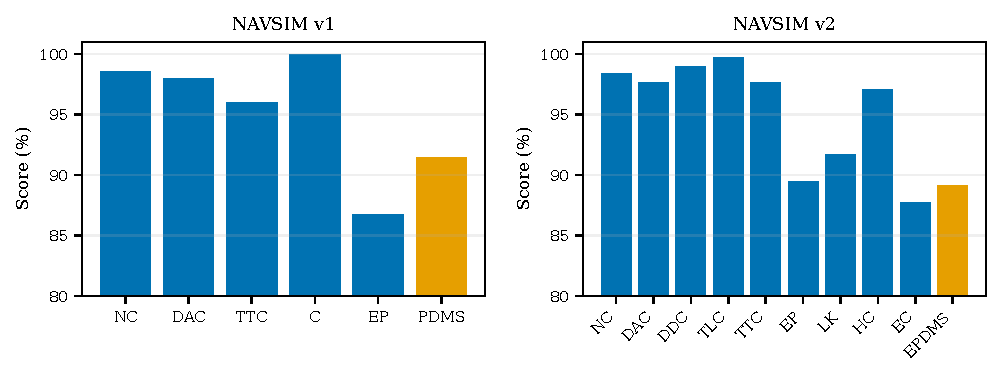
\includegraphics[width=0.76\textwidth]{figures/generated/ampt_metric_profiles.pdf}
  \caption{Scene-level reproduced AMPT component profiles on NAVSIM v1 and
  v2.  All metrics are percentages and higher is better; aggregate PDMS/EPDMS
  is shown in orange.  The profiles use 12,138 and 12,146 scored scenes,
  respectively, from one inference realization.}
  \label{fig:metric-profiles}
\end{figure*}

\paragraph{Single-trajectory inference.}
For each scene and inference seed, the model receives one observation, runs one
five-step denoising chain, and submits its single final $8\times3$ trajectory.
There is no test-time group sampling, evaluator call, candidate scoring,
reference lookup, model ensemble, or reranking.  The v1 submission provenance
independently records candidate count one, so this is a scene-level reproduced
property rather than only a methodological statement.

\paragraph{Runs and uncertainty.}
The archived v1/v2 headline exports each establish a scene-level mean for one
policy realization; they do not establish across-seed variance.  We therefore
do not attach a fabricated standard deviation to the 0.1--0.3 point increments
in the paper.  For the proposed rerun, each of seeds
20260726/20260727/20260728 produces a
complete scene export.  We first compute the mean for each run and report the
mean $\pm$ standard deviation across the three runs.  Method differences use
10,000 paired bootstrap resamples of shared scenes (resampling seeds and then
scenes within seed when multiple seeds are present), with a fixed analysis seed
of 2027 and a two-sided 95\% interval.  Recovery proportions use Wilson 95\%
intervals.  Scene bootstrap intervals from one model run describe variation
over the evaluated scenes and are explicitly not interpreted as training-seed
stability.

\paragraph{Model selection disclosure.}
The archived final v1 provenance states that \texttt{navtest} participated in
checkpoint selection.  We therefore describe the headline table as a
paper-reported benchmark comparison, not as a clean held-out model-selection
study.  The proposed rerun selects checkpoints only on the training/validation
partition, seals a checkpoint hash before \texttt{navtest}, and evaluates each
sealed hash once per inference seed.  This disclosure does not change a main
paper number; it narrows the fairness claim to what the available provenance
supports.

\subsection{The Fixed 658-Scene Recovery Protocol}
\label{sec:hard658-protocol}

The hard population is fixed before comparing optimization methods.  A scene
enters the set when the ReCogDrive IL policy receives PDMS zero in all five
sampling attempts because of collision, drivable-area violation, or both.
The resulting intersection contains 658 scene IDs.  A method \emph{recovers} a
scene when its single submitted trajectory has PDMS strictly greater than
zero under the same evaluator; the threshold is not retuned per method.

For consistency with the main paper, every supplementary hard-set analysis
uses the same archived scalar-GRPO versus historical Core-Pareto recovery pair that produced
367 and 440 positive-score scenes.  It does not substitute a later
full-benchmark checkpoint.  On the 658 fixed scenes, scalar GRPO has 367
positive and 291 zero-score outcomes, whereas the manuscript recovery
checkpoint has 440 positive and 218 zero-score outcomes.  Their paired
transition counts are 347 retained successes, 20 new failures, 93 repaired
failures, and 198 persistent failures.  Hence the net recovery is
$93-20=73$ scenes, exactly the change $440-367$, rather than a gain obtained by
hiding newly failed scenes.  The corresponding recovery rates are 55.8\%
(Wilson 95\% CI 52.0--59.5; $n=658$) and 66.9\% (63.2--70.4; $n=658$).  A
10,000-sample paired scene bootstrap gives an absolute difference of 11.1
percentage points with a 95\% interval of 8.1--14.3 points.
These intervals describe one archived checkpoint pair; no training-seed
identifier was retained for this hard-set export.

The fixed-set construction contains 480 DAC-only, 165 collision-only, and 13
joint collision-and-DAC cases according to the archived cause manifest.  The
same IDs and failure labels are used in all hard-set transition and case-table
analyses.  In particular, ``440 recovered'' means 440 positive outcomes on the
fixed original population; the transition table is required whenever the
claim is interpreted as a policy-to-policy improvement.

\subsection{Baseline and Controlled-Comparison Protocol}
\label{sec:baseline-protocol}

\begin{table*}[t]
\centering
\small
\caption{Fair-comparison protocol for main-paper baselines. All methods use one inference candidate and no test-time scorer in the paper table; unreported backbone/sensor/data details are not inferred. Result identity distinguishes reported from reproduced.}
\label{tab:baseline_protocol}
\resizebox{\textwidth}{!}{%
\begin{tabular}{lcccccc}
\toprule
method & backbone & sensors & training\_data & inference\_candidates & test\_time\_scorer & result\_identity \\
\midrule
AMPT & InternVL3-2B + ReCogDrive diffusion planner & multi-view in paper; one audited APR command resolves single camera & NAVSIM plus offline candidate/teacher pools & 1 & no & locally reproduced v1/v2 final rows; camera-manifest discrepancy disclosed \\
ReCogDrive & not disclosed in current PDF & not disclosed in current PDF & not disclosed in current PDF & 1 & no & paper reported \\
DiffusionDriveV2 & not disclosed in current PDF & not disclosed in current PDF & not disclosed in current PDF & 1 & no & paper reported \\
Drive-JEPA & not disclosed in current PDF & not disclosed in current PDF & not disclosed in current PDF & 1 & no & paper reported \\
\bottomrule
\end{tabular}%
}
\end{table*}


AMPT's v1 and v2 rows are locally reproduced from scene-level outputs.  Other
headline baseline rows are values reported in the main paper and their cited
sources; no local checkpoint, common prediction export, or common seed manifest
was found for them.  They are consequently labeled \emph{reported}, not
\emph{reproduced}.  The table records backbone, sensor interface, training
data, number of inference candidates, and use of a test-time scorer whenever
the cited evidence establishes those fields.  An unavailable field is marked
``not established by the audited source'' rather than filled by analogy with
AMPT.

For the GT/Score/Pareto/PC-MTS comparison, the paper reports a shared
initialization, diffusion SFT loss, optimizer, epoch budget, scalar-GRPO
configuration, and evaluation protocol.  The controlled reproduction
additionally seals the candidate-source manifest, fixes the proposed non-GT
sampling probability, matches the accepted candidate count, draws one target
per scene-update, and uses the same three proposed training seeds.  For Scalar GRPO versus FF-PGRPO, all rollout
chains are generated from the same initialization and sampled with the same
seed before the credit function is changed.  For No APR versus Full APR, total
optimizer steps are matched by continuing the no-APR policy with retention
targets.  These are proposed control procedures until their launch manifests
and outputs exist; the main-paper point estimates remain labeled
paper-reported.

\subsection{Reproduction and Integrity Checks}
\label{sec:reproduction-checks}

The canonical dataset stores normalized scores, benchmark and split, method,
stage, variant, round, scene ID, seed when recorded, feasibility/failure
transitions, teacher status, and its source-file/key provenance.  Validation
checks expected scene counts, duplicate scene-method records, score ranges,
the benchmark aggregate formulas, paired scene sets, and failure-state logic.
Final tables and figures are generated from that dataset; a validation failure
stops manuscript generation.  The build manifest records the command, analysis
seed, package versions, Git revision, and SHA-256 hashes of inputs and outputs.
All raw result directories are read-only, and all derived files remain under
the supplementary directory.

\section{PC-MTS Analyses: Supervision--Optimization Alignment}
\label{sec:pcmts-analysis}

This section is needed because the quality of a supervision target and its
value for subsequent policy optimization are different quantities.  PC-MTS is
designed for the latter: it keeps a target only when its score, component-wise
trade-off, local feasibility, and proximity to the frozen learner's rollout
support are jointly acceptable.  We first examine the observed
imitation-to-optimization reversal, and then specify the controls required to
separate policy compatibility from candidate count and training budget.

\subsection{The observed supervision--optimization reversal}
\label{sec:pcmts-mismatch}

Table~\ref{tab:supervision_mismatch} restates the reported comparison from the
main paper and makes the change induced by the common scalar-GRPO stage
explicit.  Score and Pareto selection produce the two strongest imitation
checkpoints (87.2 and 87.5 PDMS), yet both deteriorate under the subsequent
optimizer.  In contrast, PC-MTS deliberately gives up 0.3--0.6 imitation
points relative to those selectors and improves by 4.2 points after the same
optimization stage.  GT supervision also improves, but finishes 0.8 points
below PC-MTS.  Thus, ranking target sets by imitation PDMS would select Pareto,
whereas ranking them by optimized PDMS selects PC-MTS.  This reversal is the
direct evidence for the mismatch claimed in the paper.

\begin{table}[t]
\centering
\small
\caption{Supervision--optimization comparison on NAVSIM v1 under single-trajectory inference. All four rows are one paper-reported run; higher PDMS and GRPO change are better, and no variance is implied.}
\label{tab:supervision_mismatch}
\resizebox{\linewidth}{!}{%
\begin{tabular}{lccccc}
\toprule
method & il\_pdms & post\_scalar\_grpo\_pdms & grpo\_change\_points & evidence & runs \\
\midrule
GT & 86.4 & 90.3 & 3.9 & paper reported & 1 reported \\
Score & 87.2 & 85.8 & -1.4 & paper reported & 1 reported \\
Pareto & 87.5 & 86.7 & -0.8 & paper reported & 1 reported \\
PC-MTS & 86.9 & 91.1 & 4.2 & paper reported & 1 reported \\
\bottomrule
\end{tabular}%
}
\end{table}


\begin{figure}[t]
  \centering
  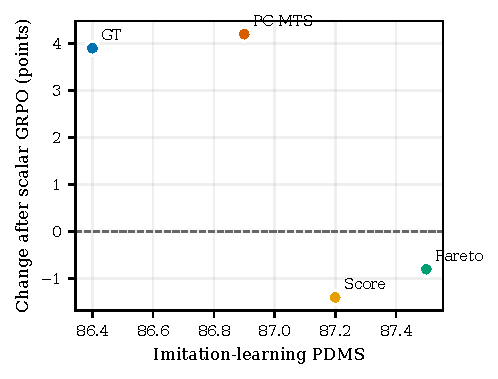
\includegraphics[width=\linewidth]{figures/generated/supervision_mismatch.pdf}
  \caption{Paper-reported imitation PDMS versus the change after the common
  scalar-GRPO stage on NAVSIM v1.  A high imitation score alone does not
  predict optimization value: Score and Pareto regress, whereas PC-MTS gains
  4.2 points.  Each marker is one reported point estimate; the paper does not
  state run/seed aggregation and no synthetic error bars are shown.}
  \label{fig:supervision-mismatch}
\end{figure}

The comparison should be interpreted at the level supported by the evidence.
It demonstrates that a higher-scoring imitation checkpoint need not be a
better starting distribution for GRPO, and that the PC-MTS set is compatible
with a large positive update in this run.  The archived paper table does not
contain scene-level outputs, acceptance counts, or multiple seeds for these
four cells.  Consequently, it does not by itself establish that the reversal
is invariant to seed, nor does it isolate candidate count from the four
filtering decisions.  We therefore do not attach synthetic error bars or
policy-distance values to these points.

\subsection{Candidate-count-matched reconstruction protocol}
\label{sec:pcmts-matched-protocol}

The released reproduction configuration turns the missing causal controls
into a predeclared, low-ambiguity experiment.  All four variants start from the
same GT-only checkpoint, use the same candidate sources, contribute exactly
one target per scene and update, train imitation learning for 200 epochs, and
then run scalar GRPO with 16 rollouts per scene for 10 epochs.  Within each
navigation-command/source stratum, accepted candidates are deterministically
subsampled to the smallest retained count across variants.  The non-GT
sampling probability is held fixed, so a method cannot receive more gradient
updates merely because it retains more candidates.  Empty strata fall back to
the logged trajectory.  In addition to final PDMS, a 300-update diagnostic
records the early GRPO gain before long-horizon training effects can dominate.

For a fully specified reconstruction when the original resolved PC-MTS
manifest is unavailable, the release marks the following as \emph{proposed
reproduction settings}, not measured settings of the reported run: a rollout
bank of 16, $K=3$ neighbors, a command-conditional 0.95 calibration quantile,
and eight temporally correlated local perturbations.  The rollout bank and
calibration queries are disjoint by construction.  Three predeclared training
seeds (20260726, 20260727, and 20260728) are used for the reconstruction, while
bootstrap seed 2027 is reserved for analysis and is never treated as an additional
training run.  These choices fill the executable configuration without
retroactively attributing unrecorded hyperparameters to the main-paper result.

For each run, the pipeline records retained candidates, acceptance rate,
candidate-source composition, feasible rollout rate, feasible high-quality
rate, all-infeasible-group rate, zero-score rate, the 10th percentile,
CVaR-10, 300-update gain, and final scalar-GRPO PDMS.  Method differences are
computed on identical scenes with a 10,000-resample paired bootstrap; means
and standard deviations are reported across the three training seeds.

\subsection{Filter attribution and sensitivity}
\label{sec:pcmts-components}

The component experiment is cumulative: (i) aggregate Score only, (ii) Score
plus the component-wise Pareto gate, (iii) the preceding gates plus calibrated
policy compatibility, and (iv) the full selector with local-feasibility
testing.  Counts are matched after each gate, rather than relaxing a stricter
gate to reach a target count.  This distinction matters: a matched count must
not reintroduce candidates that failed the mechanism being tested.  The
decisive diagnostic is not imitation PDMS alone, but whether adding a gate
raises feasible rollout density and converts the fixed-budget GRPO change from
negative to positive.

The companion sensitivity protocol varies one factor at a time: rollout-bank
size in $\{8,16,32\}$, $K$ in $\{1,3,5\}$, calibration quantile in
$\{0.90,0.95,0.975\}$, and perturbation count in $\{4,8,16\}$.  Compatibility
alternatives are compared at the same acceptance rate: candidate-to-GT
ADE/FDE, distance to the deterministic policy output, minimum rollout-bank
distance, average $K$-nearest distance, and command-calibrated $K$-nearest
distance.  These are evidence-bounded planned analyses: the release contains
their configurations and logging schema, but no unexecuted outcome is used to
support the paper's reported 91.1 PDMS.

Taken together, the existing reversal and the matched protocol close two
different parts of the argument.  The former establishes that isolated target
quality can disagree with downstream optimization value; the latter defines
the experiment needed to attribute that disagreement specifically to policy
compatibility rather than supervision quantity.

\section{FF-PGRPO Analyses: Feasibility Before Positive Credit}
\label{sec:ffpgrpo-analysis}

Aggregate reward can hide an unsafe trade: progress or comfort may increase
enough to give positive standardized advantage even when collision avoidance,
drivable-area compliance, or a protected reference metric regresses.  The
purpose of FF-PGRPO is therefore not merely to reshape the scalar score, but to
change which rollouts are eligible for positive credit.

\subsection{What the stage ablation establishes}
\label{sec:ffpgrpo-stage-ablation}

On NAVSIM v1, the no-stage baseline in the main ablation has 86.5 PDMS, 98.1
NC, 94.7 DAC, 94.2 TTC, and 80.9 EP.  Applying FF-PGRPO without PC-MTS reaches
91.0 PDMS, with 98.4 NC, 98.0 DAC, 95.8 TTC, and 85.93 EP.  With PC-MTS as the
initialization, FF-PGRPO reaches 91.1 PDMS, 98.5 NC, 98.0 DAC, 96.0 TTC, and
86.0 EP before APR.  The improvement is therefore not produced by sacrificing
the displayed hard-safety components for progress: DAC improves by 3.3 points
and TTC by 1.6 points in the FF-PGRPO-only row, while EP increases by 5.03
points.  These are paper-reported point estimates whose run/seed aggregation
is not stated, so the small 0.1-point
difference between the two FF-PGRPO rows is not presented as a stable gain.

\begin{table*}[t]
\centering
\small
\caption{Stage-wise NAVSIM v1 ablation under single-trajectory inference. Higher is better. Rows are one paper-reported run; only the final AMPT row is independently reproduced from 12,138 scene scores.}
\label{tab:stage_ablation}
\resizebox{\textwidth}{!}{%
\begin{tabular}{lcccccccccccc}
\toprule
configuration & pcmts & scalar\_grpo & ff\_pgrpo & apr & NC & DAC & TTC & C & EP & PDMS & evidence & runs \\
\midrule
GT-only & no & no & no & no & 98.1 & 94.7 & 94.2 & 100.0 & 80.9 & 86.5 & paper reported & 1 reported \\
PC-MTS & yes & no & no & no & 98.2 & 95.2 & 94.5 & 100.0 & 81.3 & 86.9 & paper reported & 1 reported \\
Scalar optimization & no & yes & no & no & 98.4 & 98.0 & 95.8 & 100.0 & 85.93 & 91.0 & paper reported & 1 reported \\
PC-MTS + FF-PGRPO & yes & no & yes & no & 98.5 & 98.0 & 96.0 & 100.0 & 86.0 & 91.1 & paper reported & 1 reported \\
Full AMPT & yes & no & yes & yes & 98.5 & 98.0 & 96.0 & 100.0 & 86.7 & 91.4 & paper reported / final row scene-reproduced & 1 reported + 12138 scenes final \\
\bottomrule
\end{tabular}%
}
\end{table*}


This result is consistent with the proposed ordering---recover feasibility,
then optimize continuous quality---but an aggregate stage ablation cannot
directly reveal the sign of individual rollout credits.  The fixed hard-scene
transition in Section~\ref{sec:hard658} provides scene-level evidence, and the
instrumentation below defines the rollout-level test.

\subsection{Credit diagnostics}
\label{sec:ffpgrpo-credit-diagnostics}

For rollout $i$, let $A_i>0$ denote positive assigned advantage and let
$V_i=1$ denote a violation of any hard-feasibility, protected-reference, or
admissible-Pareto condition.  We report
\begin{equation}
  \mathrm{PCVR} =
  \frac{\sum_i \mathbb{1}[A_i>0]V_i}
       {\sum_i \mathbb{1}[A_i>0]},
  \label{eq:positive-credit-violation}
\end{equation}
and separately count reference-regressing and Pareto-dominated positive
credits.  A denominator of zero is reported as ``no positive credits,'' not as
zero violation.  FF-PGRPO's implementation makes a violating rollout
ineligible for positive credit and exposes assertions for this contract.  The
archived training run, however, does not contain the per-rollout trace needed
to quote an observed PCVR; we do not convert a code invariant into a fabricated
measured rate.

The stepwise mechanism ablation adds: (i) the hard feasibility gate, (ii) the
coherent-reference guard, (iii) the Pareto positive-credit gate, and (iv) the
all-infeasible recovery rule.  Every variant logs group state
(all-feasible/mixed/all-infeasible), feasibility rate, positive and negative
advantage means, PCVR, reference-regressing positive-credit rate,
dominated-positive-credit rate, zero-to-feasible repair, positive-to-zero
regression, and updates until the first feasible rollout.  The coherent
reference is always one executable trajectory.  The historical
component-wise envelope remains only as an ablation because combining the best
value of each metric from different trajectories may describe no realizable
plan and can make every sampled rollout appear to regress.

The low-cost diagnostic run uses the paper's group size of 16 and stops at 300
updates; the final run uses the reported 10 epochs.  All variants share the
same sampled rollout tensors when credit is recomputed offline, which makes
the initial credit-assignment comparison independent of policy drift.  New
training is required only for the subsequent learning curves and remains
disabled unless explicitly enabled.

\subsection{Hard-scene evidence for feasibility-first recovery}
\label{sec:ffpgrpo-hard-evidence}

The manuscript recovery checkpoint is evaluated on the same 658-scene set as
scalar GRPO.  Scalar GRPO produces a positive score in 367 scenes (55.8\%,
95\% Wilson CI 52.0--59.5\%), whereas the AMPT recovery checkpoint is positive
in 440 scenes (66.9\%, CI 63.2--70.4\%).  The comparison uses a single
trajectory per scene and neither method uses test-time sampling, scoring, or
reranking.  Crucially, the paired transition is not merely a difference of
gross counts: 93 scalar-GRPO zeros become positive, 20 scalar-GRPO positives
become zero, 347 successes are retained, and 198 failures persist.  Net
recovery is therefore $93-20=73$ scenes, or 11.1 percentage points.  A
10,000-resample scene-paired bootstrap (analysis seed 2027) gives a 95\% CI of
8.1--14.3 percentage points for this paired change.  This interval quantifies
scene variation for this fixed checkpoint pair; it does not replace missing
multi-seed training uncertainty.

The subset mean PDMS increases from 0.5101 to 0.6145.  The corresponding
component means change from 0.8381 to 0.8815 for NC, 0.7052 to 0.7781 for DAC,
0.7705 to 0.8161 for TTC, and 0.4956 to 0.5932 for EP; comfort increases from
0.9985 to 1.0000, while DDC changes from 0.9567 to 0.9521.  This last decrease
is why protected metrics must be reported next to aggregate recovery rather
than summarized as universal component-wise improvement.  The complete
transition and failure-type decomposition are given in
Section~\ref{sec:hard658}.

The aggregate ablation, paired hard-scene transition, and positive-credit
instrumentation serve complementary roles.  The first shows the overall stage
gain, the second verifies that recovery is net positive rather than purchased
entirely with new failures, and the third is the predeclared test of the
claimed credit-assignment mechanism.

\section{APR Analyses: Dynamic, Policy-Relative Teachers}
\label{sec:apr-analysis}

APR addresses a moving-target problem.  A trajectory that is a useful local
teacher for the current policy can become redundant after refinement, while a
previously distant candidate can enter the policy's compatible neighborhood.
The relevant question is therefore not whether additional optimization steps
help, but whether rebuilding and re-auditing the teacher set provides useful
targets while retaining already safe behavior.

\subsection{Round-wise behavior and protected components}
\label{sec:apr-rounds}

The main paper reports a monotonic sequence of 91.10, 91.21, 91.37, and 91.45
PDMS from Round 0 through Round 3, corresponding to gains of $+0.11$, $+0.16$,
and $+0.08$.  In the stage ablation, adding APR to the PC-MTS+FF-PGRPO policy
raises PDMS from 91.1 to 91.4 and EP from 86.0 to 86.7, while the displayed NC,
DAC, TTC, and comfort values remain 98.5, 98.0, 96.0, and 100, respectively.
This pattern is aligned with APR's design: local teacher updates increase
progress without visible regression in the protected components at the
reported precision.

Each round value is a reported checkpoint summary; its run/seed aggregation is
not stated.  No across-seed
standard deviation is available, and the 0.08--0.16 point increments are not
claimed to be independently significant.  Moreover, the archived experiment
history contains accepted and rejected branches rather than a single complete
three-round hash chain; the four values above are therefore treated as the
paper's round-level summary, not as permission to infer missing intermediate
measurements.

\begin{table}[t]
\centering
\small
\caption{Paper-reported NAVSIM v1 APR progression under single-trajectory inference. Higher is better. Run/seed aggregation is not stated and no training-seed confidence interval is available.}
\label{tab:apr_rounds}
\resizebox{\linewidth}{!}{%
\begin{tabular}{lcccc}
\toprule
round & pdms & gain\_points & evidence & runs \\
\midrule
0 & 91.1 & 0.0 & paper reported & reported point; run/seed aggregation not stated \\
1 & 91.21 & 0.11 & paper reported & reported point; run/seed aggregation not stated \\
2 & 91.37 & 0.16 & paper reported & reported point; run/seed aggregation not stated \\
3 & 91.45 & 0.08 & paper reported / final score scene-reproduced & reported point + 12138 final scenes; run aggregation not stated \\
\bottomrule
\end{tabular}%
}
\end{table}


\begin{figure}[t]
  \centering
  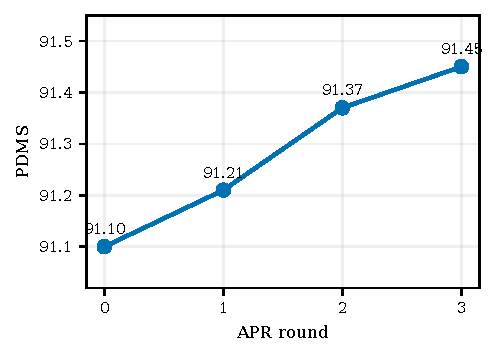
\includegraphics[width=\linewidth]{figures/generated/apr_rounds.pdf}
  \caption{Paper-reported NAVSIM v1 progression across APR rounds.  The final
  point is reproduced at scene level, but the small round increments are from
  one reported sequence and carry no across-seed error bar.}
  \label{fig:apr-rounds}
\end{figure}

\subsection{Teacher audit and post-interpolation evaluation}
\label{sec:apr-teacher-audit}

One traceable APR teacher-construction pass starts from 39,261 strict external
trajectories: 25,402 (64.7\%) from one driving-policy source and 13,859
(35.3\%) from a second source.  After interpolation with coefficient 0.25 and
exact re-evaluation, 28,910 targets remain, an acceptance rate of 73.6\%; the
remaining 10,351 are rejected.  These counts are from one audited navtrain
construction pass and are not presented as the source proportions of every
APR round.  They nevertheless establish an important operational fact:
interpolation is followed by evaluator-based admission, and the check is
non-vacuous---more than one quarter of the pre-audit union does not enter the
distillation set.

\begin{table}[t]
\centering
\small
\caption{Audited APR teacher-pool construction on NAVSIM navtrain. Counts are from one archived teacher audit; the 28,910 accepted teachers follow interpolation and exact re-evaluation. Higher acceptance is not inherently better because guards constrain quality.}
\label{tab:apr_teacher_pool}
\resizebox{\linewidth}{!}{%
\begin{tabular}{lcccc}
\toprule
step & source & count & acceptance\_definition & evidence \\
\midrule
source selection & DriVor & 25402 & source-specific strict candidates & archived APR runbook \\
source selection & DiffusionDriveV2 & 13859 & source-specific strict candidates & archived APR runbook \\
strict union & merged sources & 39261 & feasible and component-protected before interpolation & deterministic sum of audited source counts \\
post-interpolation audit & accepted teachers & 28910 & alpha 0.25 then exact re-evaluation & archived APR runbook \\
\bottomrule
\end{tabular}%
}
\end{table}


Teacher status is defined relative to the current policy.  A candidate is
\emph{accepted} when its evaluated local target is feasible, exceeds the
current single prediction by the required margin, preserves protected
metrics, and stays inside the current rollout neighborhood.  An accepted
teacher becomes \emph{expired} if it fails those tests after the policy is
updated.  A previously rejected candidate is \emph{newly activated} if it
passes after the rollout bank and current prediction are regenerated.  These
definitions prevent lifecycle counts from being conflated with raw pool size.

The interpolation search is descending: larger moves are evaluated first and
the first admissible move is retained.  Every accepted target stores the
teacher, current prediction, interpolation coefficient, post-interpolation
score, protected-metric deltas, compatibility distance, and evaluator hash.
No-interpolation and no-post-evaluation controls remove different safeguards:
the former jumps directly to the teacher, whereas the latter retains a local
trajectory without verifying that interpolation preserved feasibility.

\subsection{Step-matched controls}
\label{sec:apr-controls}

The release defines eight variants from the same Round-0 checkpoint and
matches the total number of optimizer updates: extra training on the existing
mixture, one-shot distillation, repeated use of a fixed teacher set, dynamic
teachers, dynamic teachers without interpolation, without post-interpolation
re-evaluation, without policy retention, and full APR.  The dynamic-teacher
and full-APR variants rebuild predictions, rollout banks, and teacher audits at
the same three round boundaries reported in the paper.  The fixed-teacher
variant repeats the Round-1 set without re-ranking it; the extra-training
control receives the same update count but no new teacher target.  This design
separates four possible explanations: more updates, teacher supervision in
general, teacher-set rebuilding, and the interpolation/retention safeguards.

For every round, the required report contains PDMS and all components,
regressed scenes, new failures, accepted/expired/newly activated teachers,
mean and median verified teacher advantage, interpolation-coefficient
distribution, and scene coverage.  A checkpoint is promoted only if its
single-trajectory aggregate score improves and protected metrics pass the
same non-regression audit; otherwise the previous checkpoint remains the
dynamic anchor.  Training ends after three promoted rounds or when no audited
local target remains.  These controls are configured but not represented as
measured results in this supplement, because running them would require new
training.

Optional task-vector consolidation is kept separate from teacher discovery.
The implementation can mask low-salience coordinates, require directional
agreement, bound each branch norm and the total displacement from the current
anchor, and then evaluate the merged checkpoint.  The best-branch, simple
average, task-arithmetic, and TIES-style controls are required before assigning
an independent gain to merging~\cite{taskarithmetic2023,ties2023}.  In the
absence of a stable, step-matched gain, merging should be read as a conservative
checkpoint-consolidation detail, not as the source of APR's teacher lifecycle.

The present evidence therefore supports two bounded statements: the reported
APR rounds are monotonic and preserve the displayed safety/compliance metrics,
and an audited construction pass materially filters proposed local targets
after re-evaluation.  The step-matched variants above are the necessary test
for the stronger causal claim that dynamic rebuilding, rather than additional
training alone, explains the full increment.

\begin{table}[t]
\centering
\small
\caption{APR fixed-teacher diagnostic on NAVSIM v1. The archived fixed-set continuation decreases from its 91.2766 anchor, whereas the 91.45 endpoint is the paper's compressed dynamic-round report; the rows are diagnostic rather than a step-matched causal ablation.}
\label{tab:apr_fixed_teacher}
\resizebox{\linewidth}{!}{%
\begin{tabular}{lccc}
\toprule
policy\_or\_epoch & pdms & interpretation & evidence \\
\midrule
dynamic-teacher anchor & 91.2766 & accepted dynamic-teacher checkpoint & archived APR runbook \\
fixed-set continuation epoch 0 & 91.2526 & below dynamic-teacher anchor & archived APR runbook \\
fixed-set continuation epoch 1 & 91.2311 & further below dynamic-teacher anchor & archived APR runbook \\
paper APR round 3 & 91.45 & compressed round-level paper report & paper reported \\
\bottomrule
\end{tabular}%
}
\end{table}


\section{Failure Recovery and Qualitative Diagnostics}
\label{sec:failure-qualitative}

Qualitative evidence is most useful when organized by a mechanism and tied to
scene-level metrics.  We therefore analyze the fixed hard set first, then give
traceable examples of recovered, persistent, and newly introduced failures.
All quantitative hard-set results and the mechanism-organized case table use
the same historical checkpoint pair as the main paper's 367-versus-440
recovery claim.  The final full-benchmark visualization is separately labeled
and is not used in the 658-scene recovery analysis.

\subsection{Construction of the fixed 658-scene set}
\label{sec:hard658}

The set contains 658 NAVSIM v1 scenes for which the initial ReCogDrive policy
obtained exactly zero PDMS in all five construction samples because of an
at-fault collision (NC), drivable-area violation (DAC), or both.  The set is
fixed before comparing the scalar-GRPO and AMPT recovery checkpoints.  Under
single-trajectory evaluation, scalar GRPO is positive on 367 and zero on 291
scenes; the AMPT recovery checkpoint is positive on 440 and zero on 218.

The paired $2\times2$ transition is
\begin{equation}
\begin{array}{c|cc|c}
 & \multicolumn{2}{c|}{\text{AMPT recovery checkpoint}} & \\
\text{scalar GRPO} & \text{zero} & \text{positive} & \text{row total} \\
\hline
\text{zero}     & 198 & 93  & 291 \\
\text{positive} & 20  & 347 & 367 \\
\hline
\text{column total} & 218 & 440 & 658
\end{array}.
\label{eq:hard658-transition}
\end{equation}
Hence 93 failures are repaired, 347 successes are retained, 198 failures
persist, and 20 new failures appear.  The net change is $93-20=73$, exactly the
difference between the gross positive counts $440-367$.  This distinction is
important: 440/658 is the gross recovery rate relative to the policy used to
construct the hard set, whereas 93 and 20 describe the paired transition from
scalar GRPO to the AMPT recovery checkpoint.  The resulting 11.1-percentage-
point paired improvement has a scene-bootstrap 95\% CI of 8.1--14.3 points
(10,000 resamples, seed 2027).  It is a net improvement rather than an exchange
of an equal number of old and new failures.

\begin{table}[t]
\centering
\small
\caption{Recovery on the same 658 NAVSIM v1 scenes under one archived comparison. Rates use Wilson 95\% intervals over scenes; this interval does not represent training-seed uncertainty. Higher recovery is better.}
\label{tab:failure_recovery}
\resizebox{\linewidth}{!}{%
\begin{tabular}{lcccccc}
\toprule
Method & Positive & Zero & Recovery rate (\%) & Wilson 95\% CI (\%) & Runs & Scenes \\
\midrule
Scalar GRPO & 367 & 291 & 55.8 & [52.0, 59.5] & 1 archived comparison & 658 \\
AMPT recovery checkpoint & 440 & 218 & 66.9 & [63.2, 70.4] & 1 archived comparison & 658 \\
\bottomrule
\end{tabular}%
}
\end{table}

\begin{table}[t]
\centering
\small
\caption{Paired recovery change on 658 NAVSIM v1 scenes. The 11.1-point gain has a scene-paired bootstrap interval (10,000 resamples, analysis seed 2027); higher net repair is better. One archived model pair is available.}
\label{tab:failure_net_gain}
\resizebox{\linewidth}{!}{%
\begin{tabular}{lcccccc}
\toprule
Absolute gain (pp) & Paired 95\% CI (pp) & Zero-to-positive & Positive-to-zero & Net repair & Scenes & Runs \\
\midrule
11.1 & [8.1, 14.3] & 93 & 20 & 73 & 658 & 1 archived comparison \\
\bottomrule
\end{tabular}%
}
\end{table}


\begin{figure}[t]
  \centering
  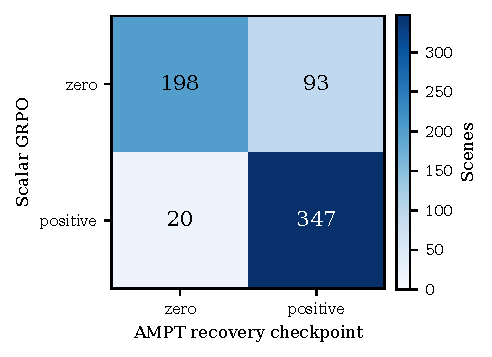
\includegraphics[width=\linewidth]{figures/generated/failure_transition.pdf}
  \caption{Scalar-GRPO to AMPT transition on the fixed 658-scene set.  The
  off-diagonal cells expose both 93 repairs and 20 regressions, rather than
  reporting gross recovery alone.}
  \label{fig:failure-transition}
\end{figure}

The original hard-set taxonomy contains 480 DAC-only scenes, 165 collision-
only scenes, 13 scenes failing both, and no residual ``other'' category.  The
paired repairs/new failures are 59/14 for DAC-only, 32/6 for collision-only,
and 2/0 for the joint category, giving net changes of 45, 26, and 2 scenes.
The gains are therefore not concentrated in only one failure type, although
the small joint category is descriptive rather than statistically decisive.

\begin{table}[t]
\centering
\small
\caption{Failure-type decomposition for the fixed 658 NAVSIM v1 scenes. Repairs and regressions use the scalar-GRPO to AMPT transition; net repairs sum to 73. One archived comparison; higher net repair is better.}
\label{tab:failure_causes}
\resizebox{\linewidth}{!}{%
\begin{tabular}{lcccc}
\toprule
Failure type & Scenes & Repairs & Regressions & Net repair \\
\midrule
DAC-only/all-fail & 480 & 59 & 14 & 45 \\
collision-only/all-fail & 165 & 32 & 6 & 26 \\
collision + DAC & 13 & 2 & 0 & 2 \\
\bottomrule
\end{tabular}%
}
\end{table}


\begin{figure}[t]
  \centering
  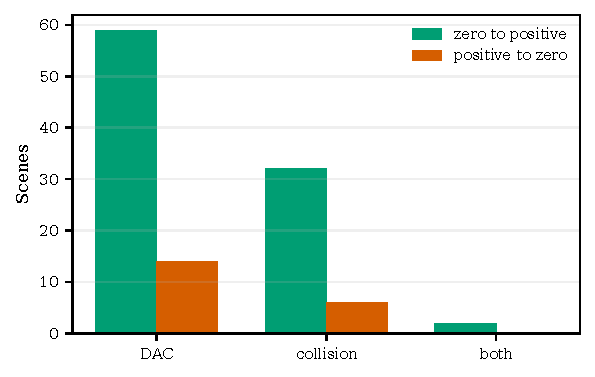
\includegraphics[width=\linewidth]{figures/generated/failure_cause_recovery.pdf}
  \caption{Repairs and regressions by the fixed hard-set cause taxonomy.  The
  net changes are 45 DAC, 26 collision, and 2 joint cases, totaling 73.}
  \label{fig:failure-causes}
\end{figure}

\subsection{Traceable scene cases}
\label{sec:traceable-cases}

Table~\ref{tab:hard658-cases} selects cases by transition type, not by visual
appeal.  Navigation commands come from the corresponding NAVSIM scene
metadata; scores and components come from the fixed paired evaluation.  The
table uses full scene identifiers so every row can be regenerated.  Component
pairs are scalar-GRPO $\rightarrow$ AMPT-recovery values.

\begin{table*}[t]
\centering
\small
\caption{Mechanism-organized examples from the fixed 658-scene set. Scene IDs and PDMS values are reproduced from the archived comparison; commands are joined from audited scene metadata. These selected cases are not an unbiased benchmark sample.}
\label{tab:hard658-cases}
\resizebox{\textwidth}{!}{%
\begin{tabular}{lccccccccc}
\toprule
Scene ID & Command & Outcome & PDMS & NC & DAC & TTC & EP & DDC & Diagnosis \\
\midrule
00fcad6d092c5e8e & left & repaired & 0.000 -> 1.000 & 0.000 -> 1.000 & 1.000 -> 1.000 & 0.000 -> 1.000 & 0.000 -> 1.000 & 1.000 -> 1.000 & Collision/TTC failure repaired without protected regression. \\
03aa8a0576a25b63 & right & repaired & 0.000 -> 0.963 & 1.000 -> 1.000 & 0.000 -> 1.000 & 1.000 -> 1.000 & 0.000 -> 0.912 & 1.000 -> 1.000 & Drivable-area failure repaired while NC and TTC remain feasible. \\
1148c72f141c532d & left & partial repair & 0.000 -> 0.583 & 0.000 -> 1.000 & 0.000 -> 1.000 & 0.000 -> 0.000 & 0.000 -> 1.000 & 1.000 -> 1.000 & Both hard failures repaired; TTC remains the limiting component. \\
00016f8b45c25a1d & left & persistent & 0.000 -> 0.000 & 1.000 -> 1.000 & 0.000 -> 0.000 & 1.000 -> 1.000 & 0.000 -> 0.000 & 0.000 -> 0.000 & DAC/progress failure persists under both audited checkpoints. \\
4b4a268bee4c5ab5 & left & regressed & 1.000 -> 0.000 & 1.000 -> 1.000 & 1.000 -> 0.000 & 1.000 -> 1.000 & 1.000 -> 0.000 & 1.000 -> 1.000 & A DAC regression creates a new zero and motivates retention. \\
\bottomrule
\end{tabular}%
}
\end{table*}


The first two cases are consistent with feasibility-oriented recovery: a hard
component changes from zero to one and positive PDMS returns.  Scene-level
before/after metrics do not identify the temporal order of training updates.
The third shows why ``recovered'' does not mean component-wise perfect.  The
fourth remains a DAC/progress failure under both audited checkpoints; without a
candidate/rollout manifest, the metrics do not identify whether pool coverage,
policy support, or optimization is responsible.  The fifth prevents
survivorship bias in the qualitative analysis and
motivates APR retention; it is one of the 20 positive-to-zero transitions
already charged against net recovery.

\subsection{Mechanism-centered visualization protocol}
\label{sec:qualitative-protocol}

The supplied renderer groups panels by decision rather than by scene
similarity.  A PC-MTS panel overlays an accepted candidate, a rejected distant
candidate, the logged trajectory, and the frozen-policy rollout neighborhood.
An FF-PGRPO mixed-group panel distinguishes unsafe, feasible-but-dominated,
and admissible Pareto-positive rollouts and prints their assigned advantages;
an all-infeasible panel shows the coherent recovery reference.  An APR panel
shows the current prediction, raw teacher, evaluated interpolant, and the
accepted/expired/newly-activated lifecycle state.  Every rendered panel reads
the scene id, command, component scores, and method name from its manifest and
uses a common legend: blue for the current prediction, green for an accepted
or positively credited trajectory, orange for a dominated/expired trajectory,
red for an unsafe trajectory, and black dashed for the coherent reference.

This protocol is also a safeguard against overinterpretation.  A camera/BEV
image is emitted only when the frame, command, all trajectories, and evaluator
record share the same scene identifier.  The metric-only cases in
Table~\ref{tab:hard658-cases} remain quantitative case studies if those visual
assets are unavailable; no unrelated camera frame or hand-drawn trajectory is
substituted merely to complete a panel.

\begin{figure*}[t]
  \centering
  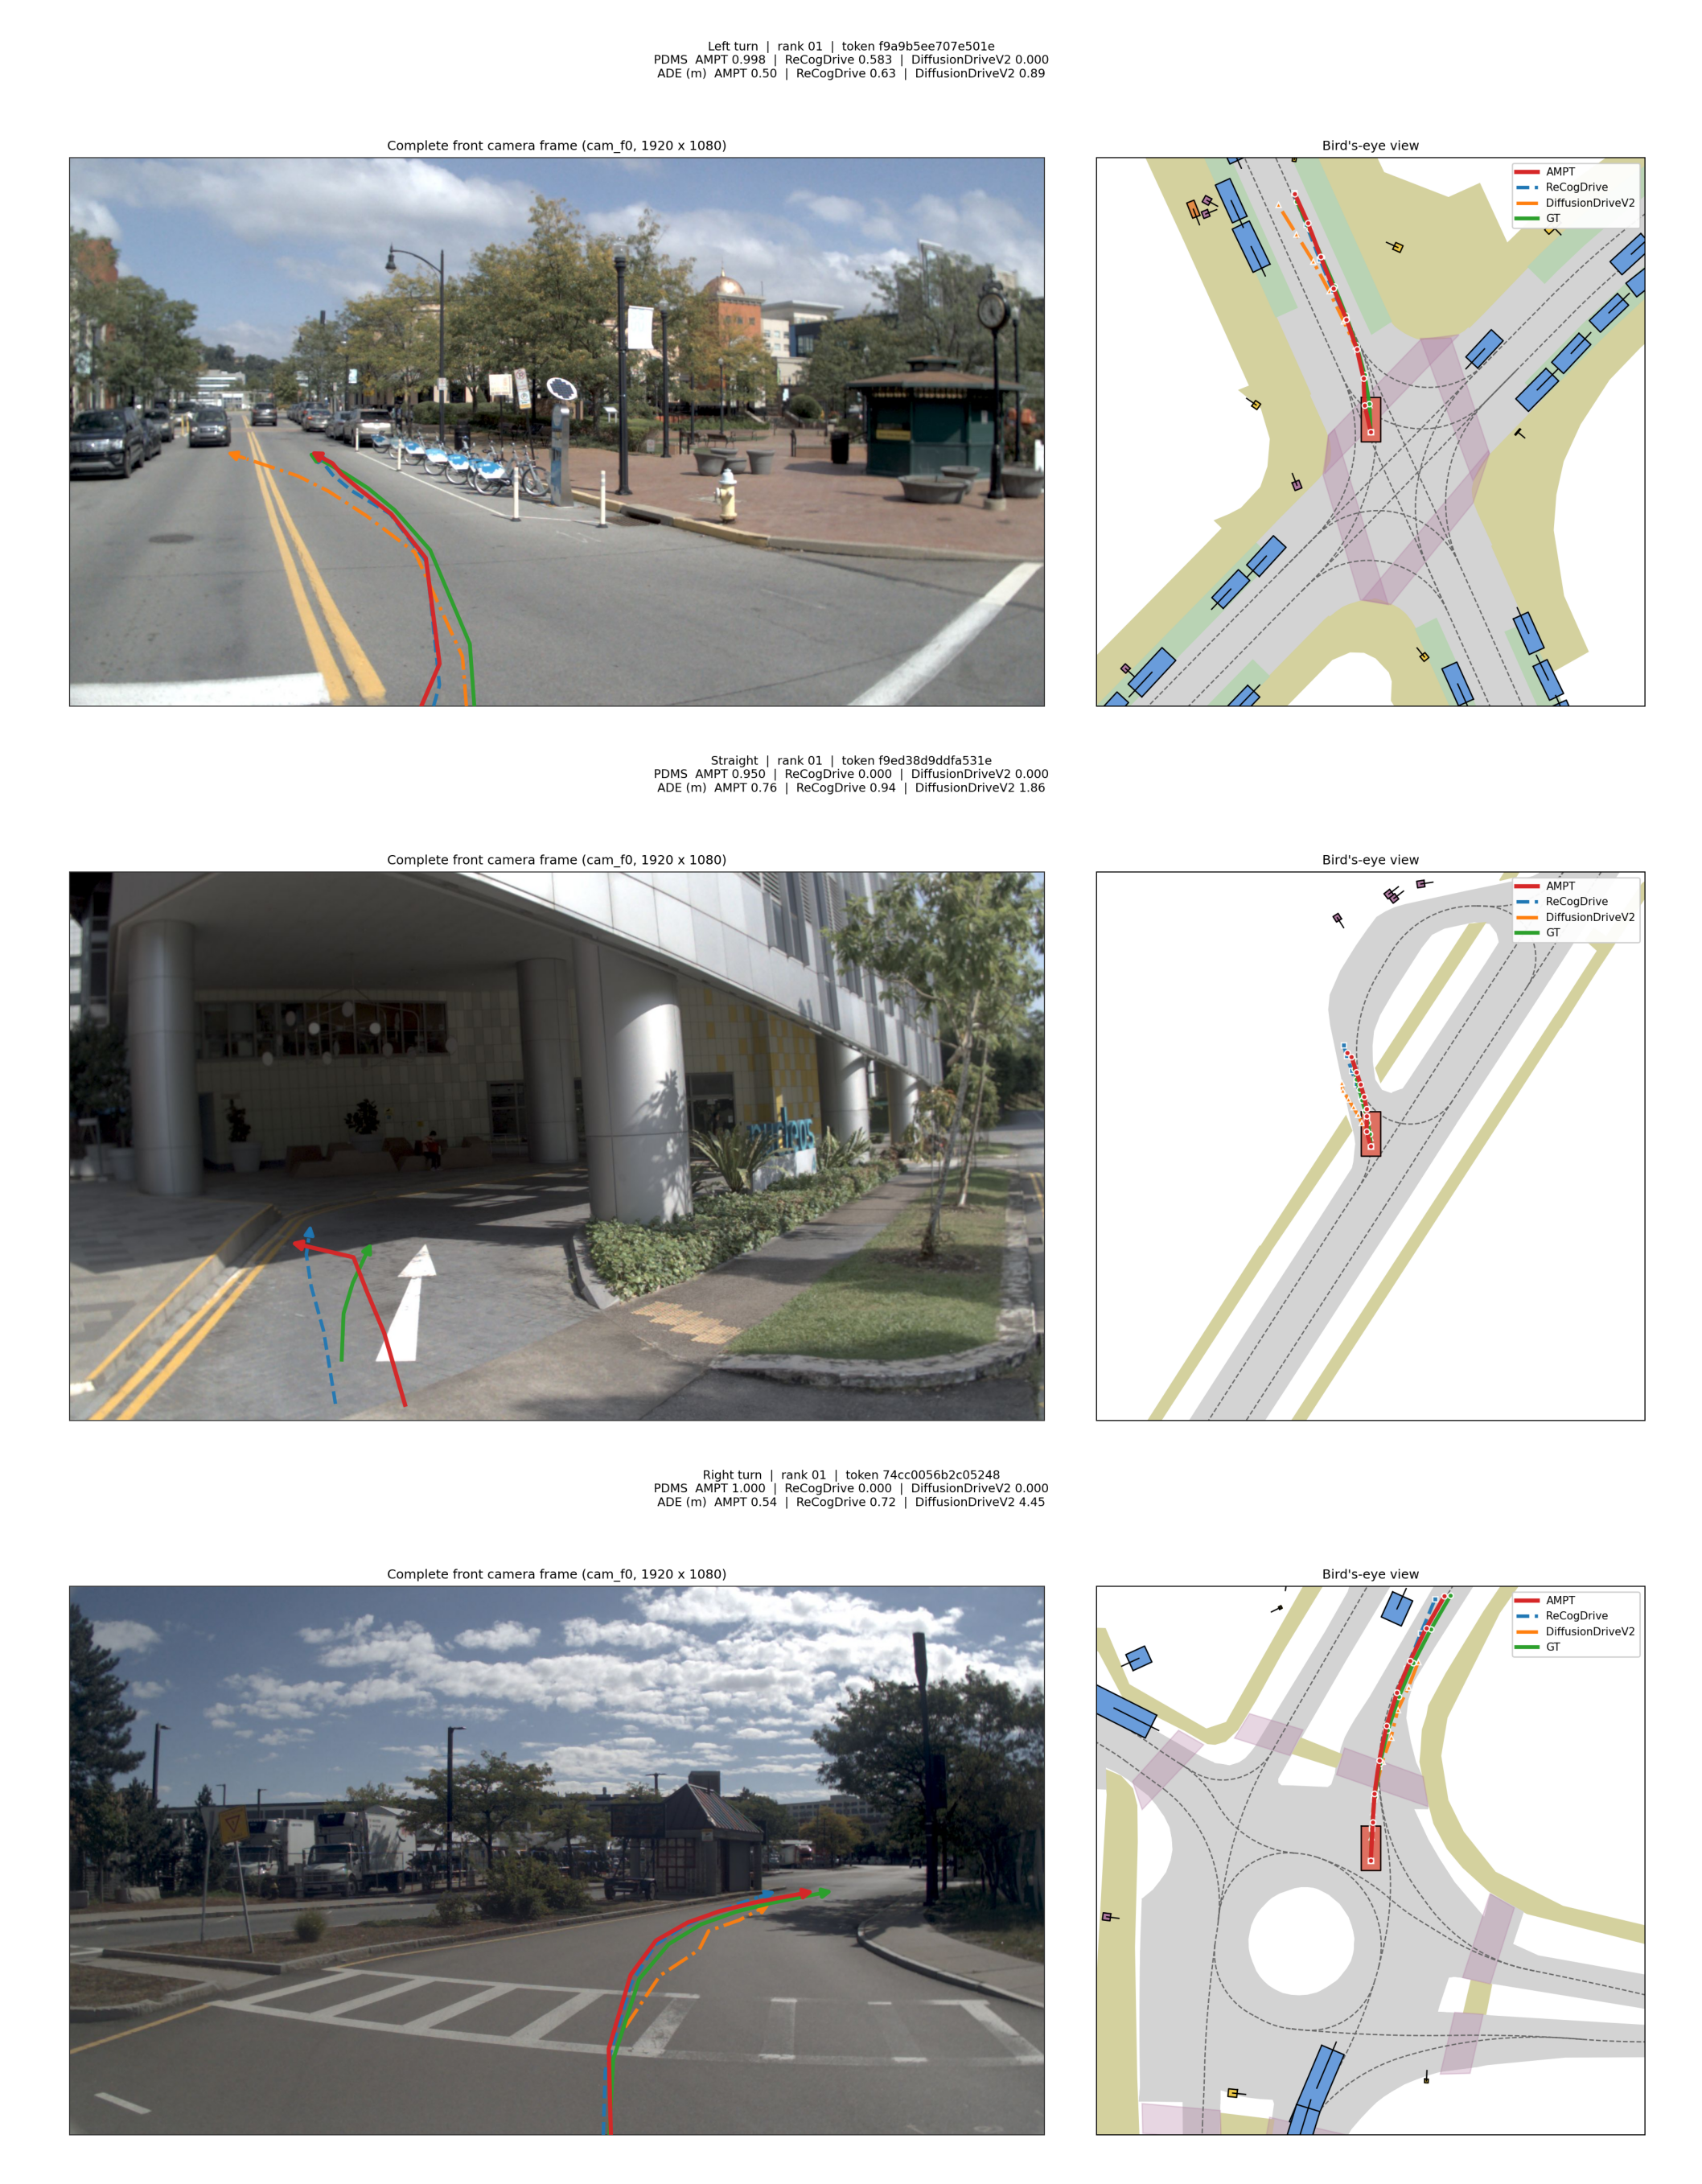
\includegraphics[width=0.92\textwidth]{figures/generated/qualitative_selected_cases.png}
  \caption{Three selected full-benchmark NAVSIM v1 cases (left, straight, and
  right commands) rendered from the separately audited final-AMPT manifest.
  Each row contains the complete front frame, bird's-eye view, scene ID,
  command, color legend, PDMS, and trajectory error.  These examples are not
  members of, and contribute no statistics to, the historical 658-scene
  recovery comparison; they illustrate final-policy behavior only.}
  \label{fig:qualitative-selected}
\end{figure*}

\clearpage

\section{Additional Related Work, Fair Comparison, and Limitations}
\label{sec:related-limitations}

\subsection{Related perspectives}

\textbf{Support-aware policy improvement.}
Conservative offline policy-improvement methods limit updates in regions where
the behavior data provide weak support.  SPIBB constrains uncertain decisions
to the baseline policy~\cite{spibb2019}, while BEAR regularizes a learned policy
toward the behavior distribution~\cite{bear2019}.  PC-MTS shares the support
intuition but applies it before optimization: it filters trajectory-level
supervision using samples from the frozen learner, with command-conditional
calibration and a local feasibility test.  It is not a general monotonic-
improvement guarantee; its role is to avoid moving the imitation policy into a
region where downstream rollout optimization has poor local support.

\textbf{Multi-objective and Pareto optimization.}
Multi-objective reinforcement learning studies policies under vector-valued
returns and alternative preference models~\cite{roijers2013}.  AMPT does not
seek a global set of Pareto-optimal policies.  PC-MTS uses a scene-local Pareto
filter for supervision, and FF-PGRPO uses a hierarchy: hard feasibility and
coherent-reference guards are evaluated before a rollout can receive positive
Pareto credit.  This order is essential when an aggregate score can compensate
for a protected regression.

\textbf{Advantage-weighted behavior learning.}
Advantage-weighted regression turns estimated advantages into weights for
supervised policy updates~\cite{awr2021}.  APR is related at the loss level,
but its weights are attached only after a candidate is compared with the
current single-trajectory prediction, locally interpolated, and re-evaluated.
Teacher admission and policy retention are therefore as important as the
weighting function itself.

\textbf{Model merging.}
Task arithmetic combines model displacements relative to a shared
anchor~\cite{taskarithmetic2023}, and TIES resolves redundancy and sign
conflicts before merging~\cite{ties2023}.  AMPT may use an anchor-constrained
variant to consolidate APR branches, but merging is optional and is separated
from teacher selection.  Passing parameter-space norm and sign checks does not
imply behavioral safety; every merged checkpoint must still undergo the same
single-trajectory evaluator audit.

\subsection{Fair-comparison boundary}
\label{sec:fair-comparison}

AMPT uses one predicted trajectory at inference.  Policy rollout banks,
candidate pools, coherent references, group sampling, specialist policies, and
the offline evaluator are training-only; there is no test-time scorer,
best-of-$N$ selection, or candidate reranking.  This contract is present in the
paper and is independently supported by the v1 submission provenance.

The released v1 scene export contains 12,138 successfully scored scenes from
12,146 predictions; the eight unscored predictions are disclosed rather than
imputed.  The v2 export contains 12,146 successful scene scores.  Its EC
aggregation follows the official evaluator, although a direct EC value is
present for 10,040 rows.  Scene-bootstrap intervals resample these scored
scenes and are explicitly labeled as scene uncertainty; they are not a
substitute for independent training runs.

The baseline rows in the main tables are treated as \emph{reported} unless a
local scene export and matching protocol are available.  AMPT's v1/v2 rows are
reproduced from scene-level outputs, but protocol matching is not established
for every external baseline.  Moreover, the audited v1 provenance records use
of navtest for checkpoint selection.  We therefore avoid a strict held-out
state-of-the-art claim and report protocol fields---backbone, sensors, training
data, inference candidates, and test-time scoring---alongside each comparison.

The 658-scene result uses the recovery checkpoint and checkpoint pair specified
by the main-paper analysis.  It is a fixed-subset diagnostic, not a claim that
every later checkpoint must induce the same transitions.  Reporting the full
$2\times2$ matrix in Eq.~\ref{eq:hard658-transition} makes the gross and net
notions of recovery explicit.

\subsection{Limitations}
\label{sec:limitations}

\textbf{Finite support estimates.}
Compatibility is estimated from a finite rollout bank.  Sparse commands or
multi-modal scenes can make a genuinely useful target appear distant, and the
calibrated neighborhood is only as representative as the frozen policy
samples.  Increasing bank size improves coverage but raises offline inference
and storage cost.

\textbf{Evaluator bias and non-reactive evaluation.}
All three stages use an offline NAVSIM evaluator for filtering, credit, or
teacher validation.  Systematic evaluator errors can therefore be amplified
across stages.  NAVSIM's non-reactive agents also cannot reveal how other road
users would respond to the learned trajectory; feasibility under this scorer
is not a closed-loop safety guarantee.

\textbf{Candidate-pool ceiling.}
APR can select and localize only behaviors represented in its multi-source
pool.  If no source proposes a valid maneuver, rebuilding the pool changes no
target.  The persistent case in Table~\ref{tab:hard658-cases} establishes
persistence under two audited checkpoints, but cannot diagnose this pool
ceiling without a per-scene candidate manifest.

\textbf{Locality can reject long-horizon value.}
The policy-compatibility filter intentionally favors learnable local targets.
It may reject a distant behavior that is initially difficult to imitate but
would be valuable after a longer curriculum.  Policy-dependent teacher-value
and cross-policy selection experiments are therefore important follow-ups.

\textbf{Benchmark-specific hierarchy.}
The ordering of NC/DAC feasibility, DDC/TLC guards, progress floors, and
continuous Pareto objectives reflects NAVSIM metrics.  Transferring AMPT to a
new benchmark requires revalidating the hierarchy and calibration thresholds,
not merely renaming metric fields.

\textbf{No behavioral semantics for parameter merging.}
Task-vector masks, direction agreement, and norm constraints bound parameter
movement but do not provide a semantic or safety guarantee.  If its independent
gain is not stable across seeds and step-matched controls, merging should
remain an implementation detail.

\textbf{Statistical scope.}
The supervision comparison, stage ablation, and APR round table are available
as reported point estimates rather than three-seed aggregates.  Small APR
increments must not be described as stable until the configured multi-seed
controls are run.  The paired 658-scene interval establishes a robust scene-
level net transition for one checkpoint pair, but does not measure training-
seed variation.

These limitations narrow rather than alter the paper's central claim.  The
currently traceable evidence establishes the supervision--optimization
reversal, a large feasibility-oriented stage gain, monotonic reported APR
rounds with preserved displayed safety components, and positive net recovery
on a fixed hard set.  Candidate-count matching, rollout-level credit traces,
step-matched APR controls, and multi-seed reruns are the remaining experiments
needed for stronger causal and stability claims.


\bibliographystyle{plain}
\bibliography{supplementary}
\end{document}
 to
% include only the appendix body from an existing manuscript preamble.
\ifdefined\AMPTMainPaper
  \makeatletter
  \def\input@path{{supplementary/}{supplementary/sections/}}
  \makeatother
  \graphicspath{{supplementary/}}
  \appendix
  \section{Additional Method Details}
\label{sec:additional-method}

This appendix makes explicit the contracts that connect the three training
stages.  This is important because the central claim of AMPT is not that a
trajectory with a high offline score is automatically a useful target, but
that supervision, rollout credit, and policy-relative refinement must agree on
what the current policy can safely learn.  We use three provenance labels
throughout.  \emph{Paper-reported} denotes a value stated in the main paper,
\emph{scene-level reproduced} denotes a value recomputed from an archived
per-scene evaluator export, and \emph{proposed reproduction} denotes a fully
specified setting for rerunning an experiment whose resolved training manifest
was not retained.  The last category is a protocol, not an observed result.

\subsection{Policy-Compatible Multi-Trajectory Supervision}
\label{sec:pc-mts-details}

\paragraph{Candidate construction and source balancing.}
For a scene $s$, let $\tau_s^0$ be the logged trajectory and let
$\mathcal C_s=\cup_m\mathcal C_s^{(m)}$ be the union of candidates supplied by
the configured proposal generators.  PC-MTS is source agnostic: a source may
be another policy seed, a structured trajectory expander, or a specialist
planner, but source identity is retained in the manifest and geometric near-
duplicates are merged before scoring.  The logged target is immutable and
is never removed.  A final Stage-1 source-count manifest was not found.  To
make the controlled reconstruction executable without presenting invented
counts as measurements, our \emph{proposed reproduction} caps every non-GT
source at eight candidates per scene before filtering.  When comparing Score,
Pareto, and PC-MTS, we use the same source
cap and retain the same number of non-GT candidates by taking the best valid
items under the corresponding rule.  Thus a difference cannot be attributed
to exposing one variant to a larger target set.

\begin{table*}[t]
\centering
\small
\caption{Candidate-source and audit budgets for PC-MTS on the NAVSIM training universe. Counts tagged proposed are reproduction settings rather than observations; higher/lower is not applicable.}
\label{tab:candidate_sources}
\resizebox{\textwidth}{!}{%
\begin{tabular}{lccccc}
\toprule
source & role & per\_scene\_budget & scene\_universe & retention\_or\_use & status \\
\midrule
Logged trajectory & immutable fallback and retention target & 1 & 103,288 expected navtrain scenes & always retained & paper-described / historical contract \\
Frozen-policy rollout bank & compatibility support estimate & 16 & 103,288-scene reproduction universe & distance calibration only & proposed reproduction setting \\
Multi-source candidate proposals & quality and Pareto targets & 8 per source & 103,288-scene reproduction universe & subject to quality/Pareto/compatibility gates & proposed reproduction budget \\
Correlated local perturbations & local feasibility audit & 8 per retained proposal & same candidate scenes & pass-rate threshold 0.75 & proposed reproduction setting \\
\bottomrule
\end{tabular}%
}
\end{table*}


\paragraph{Quality, feasibility, and Pareto filtering.}
Every complete trajectory is scored by the same offline evaluator used for
training diagnostics.  We first require hard feasibility, then a sufficient
aggregate score, and only then form the scene-wise component Pareto front.  A
candidate $a$ dominates $b$ only if it is no worse on every active Pareto
objective and is strictly better on at least one.  This order matters: a high
progress value cannot compensate for collision or leaving the drivable area.
The paper does not archive the numerical Stage-1 aggregate cutoff.  In the
\emph{proposed reproduction}, a training-split quantile is selected once so
that comparison variants are matched to the minimum retained count, followed
by a source-balanced top-$k$ tie break.  The sealed cutoff is applied
identically to all splits and is never used to synthesize a reported score.

The benchmark-specific partition is summarized below.  On NAVSIM v1, NC and
DAC are hard gates; DDC is protected; and EP, TTC, and comfort are optimized
inside the admissible region.  On NAVSIM v2, NC, DAC, DDC, and TLC are the
multiplicative compliance gates.  The historical metric adapter uses EP, TTC,
and a composite $Q=(\mathrm{LK}+\mathrm{HC}+\mathrm{EC})/3$ as its three
continuous Pareto axes; the official EPDMS report still exposes LK, HC, and EC
separately.  For binary scorer outputs the \emph{proposed reproduction}
requires a value of one up to $10^{-6}$.  The archived safety contract uses
reference-relative tolerances of $0.01$ for DDC/comfort and $0.02$ for TTC/EP;
TLC remains a hard v2 gate.  These are historical implementation values, not a
claim about the unresolved configuration of the paper checkpoint.

\begin{table}[t]
\centering
\small
\caption{NAVSIM v1/v2 metric partition used by PC-MTS and FF-PGRPO. Hard feasibility is tested before protected non-regression and Pareto quality.}
\label{tab:metric_partition}
\resizebox{\linewidth}{!}{%
\begin{tabular}{lcccc}
\toprule
benchmark & hard\_feasibility & protected\_guards & pareto\_quality & aggregate \\
\midrule
NAVSIM v1 & NC, DAC & DDC; non-regression in TTC and feasibility & EP, TTC, C & PDMS \\
NAVSIM v2 & NC, DAC, DDC, TLC & DDC/TLC feasibility; non-regression in TTC & EP, TTC, LK, HC, EC & EPDMS \\
\bottomrule
\end{tabular}%
}
\end{table}


\paragraph{Policy compatibility.}
Let $\mathcal R_s=\{\rho_j\}_{j=1}^{M}$ be rollouts sampled from the frozen
GT-only policy under the same command as the candidate.  We standardize
waypoint displacement with per-timestep, command-conditioned robust scales
fitted on the calibration split, and write the resulting trajectory distance
as $d(\tau,\rho)$.  The archived implementation additionally exposes final
displacement, heading, and velocity diagnostics, but the proposed controlled
comparison changes only the normalized waypoint statistic.  The compatibility
statistic is
\begin{equation}
 d_{\mathrm{PC}}(\tau,\mathcal R_s)
 =\frac{1}{K}\sum_{\rho\in\operatorname{NN}_{K}(\tau;\mathcal R_s)}
 d(\tau,\rho).
\end{equation}
The threshold $q_c$ is the command-specific quantile of leave-one-out policy
rollout distances on calibration scenes.  The archived code proves
leave-one-out calibration within each policy cloud, but its retained manifest
does not prove driving-log-level independence.  The proposed reconstruction
therefore enforces log-disjoint calibration and query scenes.  The paper states the general
$K$-nearest statistic but does not report $M$, $K$, or $q_c$.  The archived
implementation realizes the valid $K=1$ special case.  Our \emph{proposed
reproduction} uses $M=16$, $K=3$, and $q_c$ at the 95th percentile, with
command groups merged into a global fallback only when a command group has
fewer than 16 calibration observations.  This choice is also the center point
of the supplied sensitivity grid, rather than a retrospectively selected
result.

\paragraph{Local feasibility tube.}
Compatibility to one rollout neighborhood does not by itself establish that a
target is robust to small prediction errors.  For every candidate that passes
the previous gates, PC-MTS adds correlated perturbations to $(x,y,\psi)$ and
the implied velocity sequence.  The perturbations are sampled from normalized
policy residuals, smoothed over time, and projected back to the command-consistent
trajectory representation before exact re-evaluation.  This changes whole
trajectory segments rather than independently jittering waypoints.  The
archived implementation supports 16 or 32 perturbations; the \emph{proposed
reproduction} uses eight lower-cost perturbations, preserves the empirical
temporal covariance of policy residuals, and accepts a candidate when at least
six of eight perturbations pass
the hard feasibility gates and the protected guards.  The P1 configuration
evaluates 4/8/16 perturbations and does not tune the threshold on the test
split.

\paragraph{Target sampling and fallback.}
After filtering, the training set for scene $s$ is
$\mathcal T_s=\{\tau_s^0\}\cup\mathcal A_s$, where $\mathcal A_s$ contains
accepted candidates.  A training update draws exactly one target for the
scene, so scenes with many proposals do not receive larger gradients.  The
\emph{proposed reproduction} draws the logged target with probability $0.5$
and otherwise samples uniformly from $\mathcal A_s$; if $\mathcal A_s$ is
empty, it deterministically uses $\tau_s^0$.  Candidate identity is sampled
before the diffusion timestep, so all noisy versions in that update correspond
to a single coherent target.  Fine-tuning uses the same denoising objective as
GT-only training and produces $\pi_{\mathrm{initial}}$.

\paragraph{Implementation correspondence.}
The source-balanced builder and immutable-GT path are implemented at
\path{41a8613:navsim/agents/recogdrive/curriculum/builder.py}
and \path{41a8613:navsim/agents/recogdrive/curriculum/proposals.py}.
Physical distance and calibrated reachability are at
\path{41a8613:navsim/agents/recogdrive/curriculum/reachability.py};
the feasibility and correlated-perturbation checks are at
\path{41a8613:navsim/agents/recogdrive/curriculum/safety.py} and
\path{41a8613:navsim/agents/recogdrive/curriculum/robustness.py}.
These are historical mechanism-level implementations; the audit does not claim
that this commit is a complete hash-identical release of the final checkpoint.

\subsection{Feasibility-First Pareto GRPO}
\label{sec:ff-pgrpo-details}

\paragraph{A coherent scene reference.}
FF-PGRPO compares a rollout with one executable reference trajectory, never
with an envelope assembled from different trajectories.  The ordered source
set is: the logged trajectory, a retained PC-MTS candidate, and the current
single-trajectory prediction.  The paper-level rule selects the highest-scoring
feasible row.  The audited historical selector makes this precise by ranking
validity, hard feasibility, reference guard, robustness, core eligibility,
PDMS, distance to the current prediction, and source priority lexicographically.
Thus no higher score can bypass an earlier safety/eligibility tier.  If none is feasible, the
logged trajectory is retained only as a weak recovery target when it passes
the evaluator's basic physical checks.  Otherwise no recovery target is used
and every sampled rollout receives non-positive credit.  A component-wise
envelope is invalid because its NC, progress, and TTC values may come from
mutually incompatible plans; positive credit relative to such a synthetic
point would have no executable safety witness.

\paragraph{Group states and admissibility.}
For each scene the paper reports a group of $G=16$ policy rollouts.  We assign
the group to one of three states.  An \emph{all-feasible} group contains only
rollouts that satisfy hard feasibility; its quality statistic normalizes the
continuous score components because the binary gates are constant.  A
\emph{mixed} group contains both feasible and infeasible rollouts; feasibility
is applied first and feasible trajectories must additionally pass the coherent
reference guards.  An \emph{all-infeasible} group contains no feasible
rollout; it is not allowed to create a positive advantage by merely ranking
unsafe samples against one another.

For NAVSIM v1, admissibility requires NC and DAC and protects DDC, TTC, and an
EP floor relative to the coherent reference.  NAVSIM v2 additionally treats
DDC and TLC as hard compliance checks.  The archived safety-contract defaults
use $\mathrm{DDC}(\tau)\geq\mathrm{DDC}(r)-0.01$,
$\mathrm{TTC}(\tau)\geq\mathrm{TTC}(r)-0.02$, and
$\mathrm{EP}(\tau)\geq\mathrm{EP}(r)-0.02$.  The joint EP--TTC guard prevents
the optimizer from receiving positive credit for increasing safety merely by
stopping, or for increasing progress by collapsing the collision margin.

\paragraph{Credit assignment.}
Within a group that contains a feasible rollout, let $\widehat A_i$ be a
quality-shaped, group-relative score and let $P_i$ indicate membership in the
admissible Pareto front.  FF-PGRPO assigns
\begin{equation}
 A_i=\begin{cases}
 \max(\widehat A_i,0),
   & \substack{\text{feasible, guard-passing,}\\\text{and Pareto-positive}},\\
 \min(\widehat A_i,0),
   & \substack{\text{feasible but not}\\\text{admissible Pareto}},\\
 -\lambda_{\mathrm{unsafe}}+\min(\widehat A_i,0),
   & \text{infeasible}.
 \end{cases}
\end{equation}
Thus aggregate quality controls magnitude, whereas feasibility, a coherent
reference, and non-domination control the sign.  For mixed groups the quality
term also includes the EP-floor and joint EP--TTC penalties.  The historical
implementation preserves signs with RMS scaling rather than mean centering and
uses an archived default clip of $[-3,3]$; the \emph{proposed reproduction}
uses the predeclared sensitivity setting $[-5,5]$.

For an all-infeasible group, violation severity is the normalized sum of hard
gate deficits and protected-metric deficits.  Credit is the non-positive
within-group rank of negative severity, shifted by the unsafe penalty.  The
group loss is downweighted to $0.25$; when a valid recovery reference exists,
a diffusion recovery term with coefficient $0.25$ is added.  The proposed
regularization uses KL weight $0.02$ and anneals the BC coefficient linearly
from $0.10$ to $0.05$ over the first five epochs.  These numerical values are
historical implementation defaults and proposed rerun values, not recovered
resolved parameters for the paper's final FF-PGRPO run.

\paragraph{Diffusion credit and inference.}
One trajectory-level advantage is broadcast to every transition in that
trajectory's denoising chain.  The audited planner uses a discounted
transition-wise mean, while the paper objective writes the chain likelihood in
accumulated form; the proposed reconstruction preserves the planner reduction
and logs it in the resolved manifest.  This avoids assigning mutually
inconsistent metric credit to intermediate noisy states that are not executable
plans.  At inference, AMPT runs one denoising chain and emits one trajectory.
Group sampling, the Pareto computation, the reference selector, the offline
evaluator, and candidate reranking are absent from test time.

\paragraph{Implementation correspondence.}
Group classification, Pareto gating, violation ranking, sign-preserving
normalization, and clipping are at
\path{41a8613:navsim/agents/recogdrive/stage3_ff_pareto.py}.
The coherent-row API is at
\path{41a8613:navsim/agents/recogdrive/stage3_reference_selector.py},
and positive-credit assertions are at
\path{41a8613:navsim/agents/recogdrive/stage3_positive_credit_contract.py}.
The archived tensor layout is anchor-local; the paper-level protocol is the
union of 16 scene rollouts.  Because a final resolved layout manifest was not
found, we do not infer the number of anchors from a class default.

\subsection{Adaptive Pareto-Guided Policy Refinement}
\label{sec:apr-details}

\paragraph{Dynamic multi-source pool.}
At APR round $r$, the current policy $\pi_r$ supplies one local prediction for
every scene.  Candidate teachers come from historical policy checkpoints,
independent GRPO seeds, structured trajectory expansion, and safety-,
progress-, and regularity-oriented specialists.  Source labels survive
deduplication so per-source acceptance can be audited, but final three-round
source proportions were not archived.  The audited initial construction keeps
its observed 25,402/13,859 source mixture.  The proposed source-ablation reports
each source separately instead of claiming an unrecorded balancing rule.

\paragraph{Teacher audit.}
For a policy prediction $p_s$ and candidate teacher $t$, APR first requires
feasibility and an aggregate margin $R(t)-R(p_s)\geq m_R$.  It then applies
absolute and reference-relative protected guards.  Behavioral distance,
curvature, and jerk rank otherwise admissible teachers; they are preferences,
not claimed historical hard thresholds.  In the audited APR branch,
$m_R=0$ with a strict positive comparison, DDC has absolute floor 0.99 and
maximum drop 0.01, TTC has absolute floor 0.95 and maximum drop 0.02, and the
jerk coefficient 0.005 is a soft training regularizer.  At the interpolation
audit, the proposed reconstruction additionally applies the command-conditioned
95th-percentile compatibility calibration from PC-MTS.

\paragraph{Local interpolation and exact re-evaluation.}
An accepted teacher is not copied directly.  APR evaluates
\begin{equation}
 \tau_{s,\alpha}=p_s+\alpha(t-p_s)
\end{equation}
for a descending list of interpolation coefficients.  The first (largest)
coefficient that remains feasible, improves the aggregate score, preserves
protected metrics, and passes the current compatibility test becomes the local
target.  Every interpolated trajectory is scored anew; endpoint scores are
never linearly interpolated.  One audited branch used $\alpha=0.25$.  The
\emph{proposed reproduction} fixes the descending list to
$[1.0,0.75,0.50,0.25]$, which includes that audited setting and tests the
teacher endpoint before progressively more conservative steps.  If all
coefficients fail, the teacher is
rejected for the current round rather than kept with a smaller unscored step.

\paragraph{Weighted distillation, retention, and lifecycle.}
For verified gain $\Delta_s=R(\tau_{s,\alpha})-R(p_s)>0$, the target weight is
\begin{equation}
 w_s=\min\{5,\exp(\Delta_s/0.05)\}.
\end{equation}
The temperature $0.05$ and clip 5 are present in an audited APR training
branch.  The same diffusion denoising loss is applied to weighted local
targets, while current predictions provide retention targets with audited
weight 1.0.  At most the top one positive-advantage target is used per scene; a
scene without a valid teacher contributes retention only.  After training, the
candidate checkpoint is promoted only if aggregate validation score increases
and none of the protected aggregate components regresses beyond the audit
tolerances.  The promoted checkpoint becomes the dynamic anchor, its
predictions and rollout bank are regenerated, and the complete teacher pool is
audited again.  A previously accepted teacher is defined as \emph{expired} when
it loses its margin or guard, while a previously rejected one is \emph{newly
activated} when it passes under the new policy.  Historical scripts rebuild
round files but do not persist these labels; the proposed pipeline obtains them
by joining teacher hashes across consecutive round manifests.  The paper reports three
rounds.  The proposed stop rule is the earlier of three promotions, an empty
teacher set, or no checkpoint passing the promotion rule; it does not turn a
small unverified score fluctuation into a promotion.

\paragraph{Optional branch consolidation.}
Safety, progress, and regularity branches may be consolidated after their
teacher updates.  This is an optional checkpoint operation, not a substitute
for teacher auditing.  The audited anchor-constrained variant keeps the top
20\% salient coordinates of each base-relative task vector, removes
coordinates with inconsistent directions, clips every branch displacement to
the norm of its accepted branch, and caps total displacement at $1.05$ times
the largest accepted branch displacement.  The anchor is the current promoted
policy and is therefore updated across rounds.  If no merge candidate passes
the same evaluation guard as an ordinary APR checkpoint, the best accepted
single branch is retained.

\paragraph{Implementation correspondence.}
Teacher audits are implemented at
\path{fb96a03:scripts/stage3/build_pdms_strict_teacher_buffer.py}
and \path{fb96a03:scripts/stage3/build_pdms_safety_repair_teacher_buffer.py}.
Interpolation and exact rescoring are at
\path{ab9124c:scripts/stage3/build_pdms_blended_teacher_reference.py},
with local safety-tube checks at
\path{ab9124c:scripts/stage3/filter_pdms_teacher_reference_by_safety_tube.py}.
Retention schedules are built by
\path{fb96a03:scripts/stage3/build_pdms_teacher_refinement_schedule.py},
and the optional merge is at
\path{64f5531:scripts/stage3/merge_conflict_free_anchored_task_vector.py}.
APR is an orchestrated sequence of these audited operations; the repository
does not contain a single monolithic \texttt{APR.run} entry point.

  \section{Algorithms}
\label{sec:algorithms}

The three procedures below are separated deliberately.  PC-MTS constructs a
supervision distribution before policy optimization; FF-PGRPO assigns credit
inside one rollout group; and APR rebuilds policy-relative teachers between
training rounds.  Combining them into one loop would obscure both their
different inputs and the interfaces tested by the implementation.  A code
comment names the closest audited historical function; ``paper contract''
marks a step for which no end-to-end final-checkpoint call graph was retained.

\paragraph{Algorithm 1: Policy-Compatible Multi-Trajectory Supervision.}
\label{alg:pcmts}
\begin{quote}
\small
\textbf{Input:} logged scenes $\mathcal D=\{(o_s,\tau_s^0,c_s)\}$; candidate
sources $\{\mathcal C_s^{(m)}\}$; frozen GT policy $\pi_{\mathrm{GT}}$;
offline evaluator $E$; compatibility and robustness configuration $\xi$.

\textbf{Output:} accepted per-scene target sets $\{\mathcal T_s\}$ and the
initialized policy $\pi_{\mathrm{initial}}$.

\begin{enumerate}
  \item Load source manifests, preserve source identity, form
  $\mathcal C_s=\cup_m\mathcal C_s^{(m)}$, merge geometric near-duplicates,
  and mark
  $\tau_s^0$ immutable.  \emph{Implementation:}
  \path{41a8613:navsim/agents/recogdrive/curriculum/proposals.py:load_scene_proposals},
  \path{deduplicate_proposals}; immutable retention is enforced by
  \path{builder.py:finalize_scene_record}.

  \item Evaluate every complete candidate with $E$; reject candidates that
  fail hard feasibility, the aggregate-quality threshold, intent checks, or
  reference-relative protected guards.  \emph{Implementation:}
  \path{41a8613:navsim/agents/recogdrive/curriculum/builder.py:build_scene_intermediate},
  \path{safety.py:absolute_feasibility} and
  \path{relative_nonregression}.

  \item Compute the component-wise Pareto front among survivors and apply the
  fixed source/role quota.  Do not allow a continuous metric to restore a
  candidate removed by a hard gate.  \emph{Implementation:} component-wise
  Pareto filtering is the paper contract; the audited tree exposes the later
  role/quota step at
  \path{41a8613:navsim/agents/recogdrive/curriculum/quota_selector.py:role_aware_quota_select},
  but no separately named Pareto-front function.

  \item Sample the policy rollout cloud $\mathcal R_s$ from frozen
  $\pi_{\mathrm{GT}}$.  Fit robust distance scales and command-specific
  quantiles using leave-one-out rollout queries.  Enforce log-disjoint
  calibration/query scenes in the proposed rerun; the archived manifest proves
  leave-one-out only.  \emph{Implementation:}
  \path{41a8613:navsim/agents/recogdrive/curriculum/builder.py:_policy_cloud_for_scene},
  \path{reachability.py:fit_reachability_calibration}.

  \item For each Pareto survivor $\tau$, compute its calibrated nearest-policy
  distance $d_{\mathrm{PC}}(\tau,\mathcal R_s)$ and retain it only when the
  relevant command threshold is met.  The archived branch implements $K=1$;
  the proposed rerun sets $K$ through $\xi$.  \emph{Implementation:}
  \path{41a8613:navsim/agents/recogdrive/curriculum/reachability.py:physical_distance_components},
  \path{evaluate_reachability}.

  \item Draw temporally correlated residual trajectories around every
  compatibility-passing candidate, score each perturbation with $E$, and keep
  the center candidate only if the required fraction remains feasible and
  guard-passing.  \emph{Implementation:}
  \path{41a8613:navsim/agents/recogdrive/curriculum/robustness.py:CorrelatedErrorModel.sample_perturbations},
  \path{evaluate_robustness_tube}.

  \item Set $\mathcal T_s=\{\tau_s^0\}\cup\mathcal A_s$.  If no non-GT
  candidate survives, set $\mathcal T_s=\{\tau_s^0\}$; never borrow a target
  from another scene.  \emph{Implementation:}
  \path{41a8613:navsim/agents/recogdrive/curriculum/builder.py:finalize_scene_record}.

  \item At each visit to $s$, sample exactly one member of $\mathcal T_s$
  according to the fixed GT/candidate mixture and then sample one diffusion
  timestep.  \emph{Implementation:}
  \path{41a8613:navsim/agents/recogdrive/stage2_role_sampler.py},
  \path{stage2_bridge.py}.

  \item Fine-tune a copy of $\pi_{\mathrm{GT}}$ with the unchanged diffusion
  noise-prediction loss and return it as $\pi_{\mathrm{initial}}$.
  \emph{Implementation:}
  \path{41a8613:navsim/agents/recogdrive/first_drive_v7_planner.py}.
\end{enumerate}
\end{quote}

\paragraph{Algorithm 2: Feasibility-First Pareto GRPO Credit Assignment.}
\label{alg:ffpgrpo}
\begin{quote}
\small
\textbf{Input:} scene $o_s$; policy $\pi_\theta$; the paper's $G=16$ sampled
denoising chains and final trajectories $\{(z_i,\tau_i)\}_{i=1}^{G}$; logged,
retained, and current-policy reference candidates; evaluator $E$; credit
configuration $\zeta$.

\textbf{Output:} trajectory advantages $\{A_i\}$ and the regularized
FF-PGRPO loss.

\begin{enumerate}
  \item Convert exact evaluator outputs for every $\tau_i$ to hard-feasibility,
  continuous-quality, protected-guard, and violation-severity tensors.
  \emph{Implementation:}
  \path{41a8613:navsim/agents/recogdrive/stage3_metric_adapter.py}.

  \item Rank complete logged, retained, and current-policy rows
  lexicographically by validity, hard feasibility, reference guard,
  robustness, core eligibility, PDMS, distance, and fixed source priority;
  choose the first row $r_s$.  Never take a different trajectory for each
  reference component.  Record whether a safe recovery reference is
  available.  \emph{Implementation:}
  \path{41a8613:navsim/agents/recogdrive/stage3_reference_selector.py:CoherentReferenceSelector.select},
  \path{gather_reference_rows}.

  \item Classify the rollout group as \textsc{all-safe}, \textsc{mixed}, or
  \textsc{no-safe}.  For safe rollouts, evaluate coherent-reference guards and
  admissible Pareto membership.  The audited function consumes anchor-local
  $[B,K,R]$ tensors; the final $K\times R$ layout is unresolved, so the proposed
  rerun seals $K=8,R=2$ to preserve $G=16$.  \emph{Implementation:}
  \path{41a8613:navsim/agents/recogdrive/stage3_ff_pareto.py:classify_group_state},
  \path{anchor_local_pareto}.

  \item If the state is \textsc{all-safe}, form $\widehat A_i$ from only the
  continuous score terms.  If it is \textsc{mixed}, form $\widehat A_i$ from
  aggregate quality plus EP-floor and joint EP--TTC shaping.  Preserve the
  scene grouping during normalization.  \emph{Implementation:}
  \path{41a8613:navsim/agents/recogdrive/stage3_ff_pareto.py:FeasibilityFirstCreditAssigner.compute}.

  \item For an \textsc{all-safe} or \textsc{mixed} group, set positive credit
  only for safe, guard-passing, Pareto trajectories; clamp safe dominated or
  guard-failing trajectories to non-positive credit; and apply an additional
  unsafe penalty to infeasible trajectories.  \emph{Implementation:}
  \path{41a8613:navsim/agents/recogdrive/stage3_ff_pareto.py:FeasibilityFirstCreditAssigner.compute}.

  \item For a \textsc{no-safe} group, rank negative violation severity and
  assign only non-positive credit.  Downweight the group and, if $r_s$ is a
  valid recovery reference, add weak diffusion supervision toward $r_s$.
  \emph{Implementation:}
  \path{41a8613:navsim/agents/recogdrive/stage3_ff_pareto.py:FeasibilityFirstCreditAssigner.compute};
  the exact final recovery-loss integration is not retained.

  \item Apply sign-preserving RMS scaling and symmetric clipping.  Assert that
  no positive-credit rollout is infeasible, dominated, reference-regressing,
  or drawn from a no-safe group; log both numerator and denominator of every
  violation rate.  \emph{Implementation:}
  \path{41a8613:navsim/agents/recogdrive/stage3_ff_pareto.py:rms_scale_without_mean_centering},
  \path{stage3_positive_credit_contract.py:assert_positive_credit_contract}.

  \item Broadcast $A_i$ over the transitions of chain $z_i$, compute the
  planner's discounted transition-wise mean, and optimize it with KL/BC and
  optional recovery losses.  No evaluator or group operation is exported to
  inference.  \emph{Implementation:} the historical transition reduction is in
  \path{41a8613:navsim/agents/recogdrive/first_drive_v7_planner.py}; the audited
  commit does not expose a verified end-to-end call from that planner to
  \path{FeasibilityFirstCreditAssigner}.
\end{enumerate}
\end{quote}

\paragraph{Algorithm 3: Adaptive Pareto-Guided Policy Refinement.}
\label{alg:apr}
\begin{quote}
\small
\textbf{Input:} FF-PGRPO policy $\pi_0$; multi-source teacher pool
$\mathcal P$; evaluator $E$; interpolation list $\mathcal L$; number of rounds
$R=3$; audit and promotion configuration $\eta$.

\textbf{Output:} promoted single-trajectory policy $\pi_R$ and a round-wise
teacher lifecycle manifest derived by joining teacher hashes.

\begin{enumerate}
  \item At round $r$, run $\pi_r$ once on every training scene and cache the
  prediction, score components, trajectory geometry, and rollout-neighborhood
  calibration as the dynamic anchor.  \emph{Implementation:} policy inference
  and evaluator exports precede
  \path{fb96a03:scripts/stage3/build_pdms_teacher_refinement_schedule.py:make_refinement_schedule},
  which consumes rather than creates those cached predictions.

  \item Load and deduplicate candidates from historical policies, independent
  GRPO seeds, structured expansion, and safety/progress/regularity specialists.
  Retain source and trajectory hashes in every record.  \emph{Implementation:}
  \path{ab9124c:scripts/stage3/build_pdms_external_safety_repair_teacher_buffer.py:choose_external_safety_teachers}.

  \item Relative to the current prediction, reject a candidate unless it is
  feasible, clears the score margin, and preserves protected metrics.  Rank
  survivors by verified gain and then by smaller behavioral distance,
  curvature, and jerk; select at most one teacher for the scene.  These last
  quantities are preferences, not claimed historical hard gates.
  \emph{Implementation:}
  \path{fb96a03:scripts/stage3/build_pdms_strict_teacher_buffer.py:_strict_teacher_upgrade},
  \path{build_teacher_record}.

  \item For the selected teacher $t_s$, test
  $p_s+\alpha(t_s-p_s)$ in descending $\alpha\in\mathcal L$.  Score every
  interpolation with $E$ and choose the largest one that remains feasible,
  improves score, preserves guards, and remains policy compatible.  If none
  passes, create no teacher target for $s$.  \emph{Implementation:} the audited
  script evaluates one supplied $\alpha$ per invocation; descending search is
  the proposed outer orchestration around
  \path{ab9124c:scripts/stage3/build_pdms_blended_teacher_reference.py:blend_trajectory},
  \path{_score_one}, \path{accept_scored_teacher}.

  \item Assign each verified target the clipped exponential advantage weight
  and construct a teacher/retention schedule that records source identity.
  Scenes without
  an accepted target contribute only their current prediction as retention.
  \emph{Implementation:} weighting is in
  \path{ab9124c:navsim/agents/recogdrive/recogdrive_diffusion_planner.py};
  retention sampling is in
  \path{fb96a03:scripts/stage3/build_pdms_teacher_refinement_schedule.py:make_refinement_schedule}.

  \item Fine-tune the diffusion planner with weighted teacher loss, retention
  loss, and KL/distillation control.  If specialist branches are enabled,
  train each from the same dynamic anchor and with the same step budget.
  \emph{Implementation:}
  \path{ab9124c:scripts/stage3/launch_pdms91_external_teacher_retention_3ep.sh}.

  \item Optionally consolidate accepted specialist branches using salient,
  direction-consistent coordinates and an anchor-relative norm bound; also
  retain every unmerged branch as a promotion candidate.  \emph{Implementation:}
  \path{64f5531:scripts/stage3/merge_conflict_free_anchored_task_vector.py:conflict_free_anchored_graft}.

  \item Evaluate all candidates with single-trajectory inference.  Promote
  only a candidate that improves aggregate validation score without violating
  protected-component tolerances; otherwise keep $\pi_r$.  Record the input,
  output, and evaluator hashes.  \emph{Implementation:}
  \path{ba5908d:navsim/planning/script/run_pdm_score_from_submission.py:run_pdm_score}
  for NAVSIM v1 and
  \path{ab9124c:scripts/evaluation/score_recogdrive_predictions_navsim_v2.py:main}
  for NAVSIM v2.

  \item Rebuild the pool relative to the promoted policy.  Mark teachers that
  no longer pass as expired and previously rejected candidates that now pass as
  newly activated by joining source/trajectory hashes across consecutive
  manifests.  Stop after $R$ rounds or earlier if the teacher set is empty
  or no checkpoint passes promotion.  Return the last promoted policy, not the
  numerically largest unguarded branch.  \emph{Implementation:} the historical
  scripts rebuild each round but do not emit lifecycle labels; the proposed
  manifest join supplies them.  No monolithic APR entry point is claimed.
\end{enumerate}
\end{quote}

  \section{Implementation and Evaluation Protocol}
\label{sec:implementation}

This section separates the protocol that produced the paper's reported results
from settings chosen to make the released reconstruction executable.  It also
defines the unit of inference and the failure-recovery population; without
these distinctions, additional samples, evaluator-guided reranking, or a
different 658-scene checkpoint pair could silently change the claim being
tested.

\subsection{Architecture and Trajectory Interface}
\label{sec:architecture}

AMPT uses the paper-reported InternVL3-2B visual-language backbone and the
ReCogDrive conditional diffusion planner.  The paper describes multi-view
camera features, ego state and motion history, and a discrete high-level
command.  One audited APR command instead resolves \texttt{cam\_type=single};
because the exact final checkpoint manifest is incomplete, this is recorded as
a protocol discrepancy rather than silently attributed to every reported row.
The planning head predicts a four-second ego trajectory as eight
poses at 0.5-second spacing, stored as an $8\times3$ tensor of local-frame
$(x,y,\mathrm{heading})$.  The VLM context conditions every diffusion step;
the supervised objective samples a noisy version of one target trajectory and
regresses the corresponding diffusion noise.

The archived agent configuration sets \texttt{train\_backbone=false} and the
planner accepts cached VLM features.  Accordingly, the \emph{proposed
reproduction} freezes InternVL3-2B and optimizes the ReCogDrive diffusion
planner in all four training phases.  This makes the supervision variants
differ only in target construction and makes the policy-optimization variants
differ only in credit and refinement.  The archived planner default uses five
DDIM denoising steps; the proposed rerun keeps five steps for rollout sampling,
log-probability evaluation, and final inference.  A random training diffusion
timestep is still used for ordinary denoising supervision.

\subsection{Stage-Wise Training Protocol}
\label{sec:training-protocol}

The main paper reports 200 epochs for GT-only and multi-trajectory imitation
learning, 16 rollouts per scene and 10 epochs for GRPO, three APR rounds, and
eight NVIDIA A800 GPUs.  An archived historical Core-Pareto launcher contains
20 epochs; because it is not the resolved manifest for the reported run, it is
not used to overwrite the paper's 10-epoch protocol.  One audited APR branch
used AdamW, BF16, four GPUs, per-GPU batch size eight (global batch 32), learning
rate $5\times10^{-7}$ with minimum $2.5\times10^{-7}$, three epochs, advantage
temperature 0.05, and weight clip 5.  We identify those values as
\emph{branch-verified}, not as proof that every reported APR round used an
identical schedule.

The table marks each row as reported, branch-verified, historical, or
\emph{proposed reproduction}.  Where the final manifest is unresolved, the
proposed schedule uses AdamW with $(\beta_1,\beta_2)=(0.9,0.95)$, weight decay
$10^{-4}$, BF16, norm clipping at 1.0, and cosine decay.  GT-only and PC-MTS use
learning rate $10^{-4}$, a three-epoch warmup, minimum learning rate $10^{-6}$,
eight scenes per GPU and two-step gradient accumulation on eight GPUs (global
batch 128).  FF-PGRPO uses $10^{-4}$, two groups per GPU, four-step
accumulation on eight GPUs (64 scene groups per update), the paper's 16
rollouts per group, and the regularization schedule in
Section~\ref{sec:ff-pgrpo-details}.  APR follows the branch-verified optimizer
settings and trains three epochs per promoted round.  Proposed training seeds
are 20260726, 20260727, and 20260728; they are future rerun identifiers and are not assigned
to any existing point estimate.

\begin{table*}[t]
\centering
\small
\caption{Stage-wise training protocol. Reported/reproduced settings are distinguished from bounded reproduction settings; `not recorded' is an explicit provenance value, not a blank. Inference always emits one trajectory.}
\label{tab:stage_hyperparameters}
\resizebox{\textwidth}{!}{%
\begin{tabular}{lccccc}
\toprule
field & GT-only & PC-MTS & FF-PGRPO & APR & status \\
\midrule
Target & logged GT & one sampled GT/candidate & sampled policy trajectories & audited teacher + policy retention & mixed provenance \\
Epochs & 200 & 200 & 10 & 3 per audited branch; 3 paper rounds & paper reported / APR branch reproduced \\
Optimizer & AdamW & AdamW & AdamW & AdamW & historical implementation / reproduction setting \\
Peak learning rate & 1e-4 & 1e-4 & 1e-4 & 5e-7 & historical configs / APR reproduced \\
Minimum learning rate & 1e-6 & 1e-6 & 1e-6 & 2.5e-7 & historical configs / APR reproduced \\
Weight decay & 1e-4 & 1e-4 & 1e-4 & 1e-4 & historical / proposed for APR \\
Batch per GPU & 8 & 8 & 2 & 8 & historical / FF and APR manifests \\
GPUs & 8 & 8 & 8 & 4 & paper reports 8 overall; APR branch used 4 \\
Gradient accumulation & 2 & 2 & 4 & 1 & historical / FF and APR manifests \\
Effective batch & 128 & 128 & 64 & 32 & deterministic from rows above \\
Precision & bf16-mixed & bf16-mixed & bf16-mixed & bf16-mixed & historical / APR reproduced \\
Warmup epochs & 3 & 3 & not recorded & 0 & historical / APR reproduced \\
Gradient clipping & 1.0 & 1.0 & 1.0 & 1.0 & historical / proposed where unresolved \\
Rollouts per scene & not applicable & 16 support rollouts & 16 & 8 offline candidates & proposed PC-MTS; paper FF; APR manifest \\
Advantage temperature & not applicable & not applicable & group normalized & 0.05 & APR reproduced \\
Advantage/weight clip & not applicable & not applicable & 3.0 & 5.0 & historical FF default / APR reproduced \\
BC or retention weight & not applicable & not applicable & 0.10 to 0.05 & 1.0 retention & archived FF / APR reproduced \\
Reference KL & not applicable & not applicable & 0.02 & 0.02 prior distance & archived FF / APR reproduced \\
Inference trajectories & 1 & 1 & 1 & 1 & paper and submission provenance \\
\bottomrule
\end{tabular}%
}
\end{table*}


No new multi-GPU training was started for this supplement.  The launchers are
dry-run by default and require both \texttt{ALLOW\_TRAIN=1} and an explicit
\texttt{--execute} flag.  Wall-clock time and
storage are explicitly recorded as \emph{not measured}; no scheduler estimate
is presented as an experiment.  Offline cost is reported in evaluator calls
rather than guessed wall
time: one call per retained scene trajectory for a benchmark evaluation, eight
additional calls per Stage-1 robustness center under the proposed tube, and at
most four calls per APR teacher under the proposed interpolation list.  Every
future launch records wall time, peak device memory, output bytes, resolved
configuration, Git revision, and SHA-256 hashes.

\subsection{Benchmark Evaluation}
\label{sec:evaluation-protocol}

\paragraph{NAVSIM v1.}
The scene-level reproduced export contains 12,146 single-trajectory predictions
on \texttt{navtest}; 12,138 have metric caches and are scored.  Their mean is
PDMS 0.9145046521, with NC 0.9852941176, DAC 0.9798978415, TTC
0.9600428407, comfort 1.0, and EP 0.8674798204.  These reproduce the rounded
91.4/98.5/98.0/96.0/100/86.7 row in the main paper.  The archived inference
seed is 20260726.  The eight unscored predictions are excluded from component
and aggregate means and remain listed in provenance; they are not imputed.
The scorer implementation is mapped to
\path{ba5908d:navsim/evaluate/pdm_score.py:pdm_score}.

\paragraph{NAVSIM v2.}
The reproduced \texttt{navtest} export has 12,146 successful trajectories and
mean EPDMS 0.8911677436.  Its component means reproduce the rounded main-paper
row: NC 98.4, DAC 97.7, DDC 99.0, TLC 99.7, TTC 97.7, EP 89.4, LK 91.7, HC
97.1, and EC 87.7.  The official evaluator revision recorded with this export
is \texttt{0a380a9063d7162ec93d0f51e9990ebac585f720}.  EC has 10,040 direct
per-scene values and is aggregated by the official evaluator; we do not
pretend that the other 2,106 rows contain directly observed EC entries.

\begin{table*}[t]
\centering
\small
\caption{Scene-level reproduction of the AMPT main results under one-trajectory inference without test-time scoring or reranking. All metrics are percentages and higher is better. NAVSIM v1 has 12,138 scored scenes; v2 has 12,146.}
\label{tab:reproduced_main}
\resizebox{\textwidth}{!}{%
\begin{tabular}{lccccccccccccccc}
\toprule
Benchmark & Scenes & Inference & Runs & NC & DAC & TTC & C & EP & PDMS & DDC & TLC & LK & HC & EC & EPDMS \\
\midrule
NAVSIM v1 & 12138 & 1 trajectory & 1 archived inference seed & 98.53 & 97.99 & 96.00 & 100.00 & 86.75 & 91.45 & not recorded & not recorded & not recorded & not recorded & not recorded & not recorded \\
NAVSIM v2 & 12146 & 1 trajectory & 1 export; seed not recorded & 98.42 & 97.69 & 97.66 & not recorded & 89.45 & not recorded & 99.00 & 99.71 & 91.73 & 97.09 & 87.74 & 89.12 \\
\bottomrule
\end{tabular}%
}
\end{table*}


\begin{figure*}[t]
  \centering
  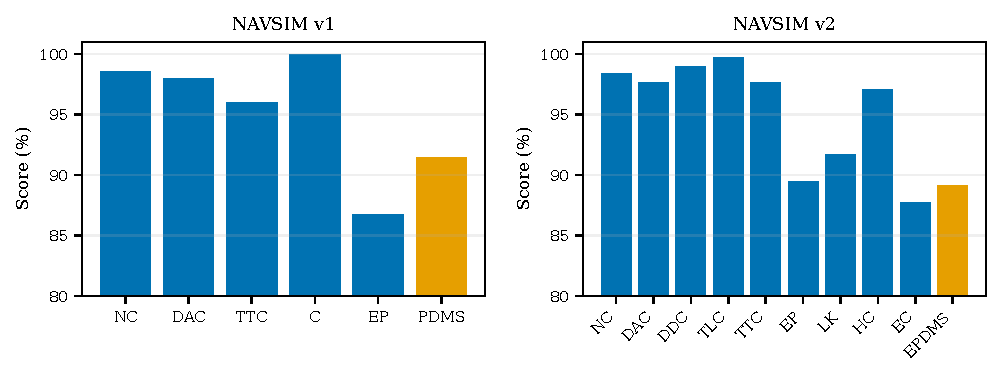
\includegraphics[width=0.76\textwidth]{figures/generated/ampt_metric_profiles.pdf}
  \caption{Scene-level reproduced AMPT component profiles on NAVSIM v1 and
  v2.  All metrics are percentages and higher is better; aggregate PDMS/EPDMS
  is shown in orange.  The profiles use 12,138 and 12,146 scored scenes,
  respectively, from one inference realization.}
  \label{fig:metric-profiles}
\end{figure*}

\paragraph{Single-trajectory inference.}
For each scene and inference seed, the model receives one observation, runs one
five-step denoising chain, and submits its single final $8\times3$ trajectory.
There is no test-time group sampling, evaluator call, candidate scoring,
reference lookup, model ensemble, or reranking.  The v1 submission provenance
independently records candidate count one, so this is a scene-level reproduced
property rather than only a methodological statement.

\paragraph{Runs and uncertainty.}
The archived v1/v2 headline exports each establish a scene-level mean for one
policy realization; they do not establish across-seed variance.  We therefore
do not attach a fabricated standard deviation to the 0.1--0.3 point increments
in the paper.  For the proposed rerun, each of seeds
20260726/20260727/20260728 produces a
complete scene export.  We first compute the mean for each run and report the
mean $\pm$ standard deviation across the three runs.  Method differences use
10,000 paired bootstrap resamples of shared scenes (resampling seeds and then
scenes within seed when multiple seeds are present), with a fixed analysis seed
of 2027 and a two-sided 95\% interval.  Recovery proportions use Wilson 95\%
intervals.  Scene bootstrap intervals from one model run describe variation
over the evaluated scenes and are explicitly not interpreted as training-seed
stability.

\paragraph{Model selection disclosure.}
The archived final v1 provenance states that \texttt{navtest} participated in
checkpoint selection.  We therefore describe the headline table as a
paper-reported benchmark comparison, not as a clean held-out model-selection
study.  The proposed rerun selects checkpoints only on the training/validation
partition, seals a checkpoint hash before \texttt{navtest}, and evaluates each
sealed hash once per inference seed.  This disclosure does not change a main
paper number; it narrows the fairness claim to what the available provenance
supports.

\subsection{The Fixed 658-Scene Recovery Protocol}
\label{sec:hard658-protocol}

The hard population is fixed before comparing optimization methods.  A scene
enters the set when the ReCogDrive IL policy receives PDMS zero in all five
sampling attempts because of collision, drivable-area violation, or both.
The resulting intersection contains 658 scene IDs.  A method \emph{recovers} a
scene when its single submitted trajectory has PDMS strictly greater than
zero under the same evaluator; the threshold is not retuned per method.

For consistency with the main paper, every supplementary hard-set analysis
uses the same archived scalar-GRPO versus historical Core-Pareto recovery pair that produced
367 and 440 positive-score scenes.  It does not substitute a later
full-benchmark checkpoint.  On the 658 fixed scenes, scalar GRPO has 367
positive and 291 zero-score outcomes, whereas the manuscript recovery
checkpoint has 440 positive and 218 zero-score outcomes.  Their paired
transition counts are 347 retained successes, 20 new failures, 93 repaired
failures, and 198 persistent failures.  Hence the net recovery is
$93-20=73$ scenes, exactly the change $440-367$, rather than a gain obtained by
hiding newly failed scenes.  The corresponding recovery rates are 55.8\%
(Wilson 95\% CI 52.0--59.5; $n=658$) and 66.9\% (63.2--70.4; $n=658$).  A
10,000-sample paired scene bootstrap gives an absolute difference of 11.1
percentage points with a 95\% interval of 8.1--14.3 points.
These intervals describe one archived checkpoint pair; no training-seed
identifier was retained for this hard-set export.

The fixed-set construction contains 480 DAC-only, 165 collision-only, and 13
joint collision-and-DAC cases according to the archived cause manifest.  The
same IDs and failure labels are used in all hard-set transition and case-table
analyses.  In particular, ``440 recovered'' means 440 positive outcomes on the
fixed original population; the transition table is required whenever the
claim is interpreted as a policy-to-policy improvement.

\subsection{Baseline and Controlled-Comparison Protocol}
\label{sec:baseline-protocol}

\begin{table*}[t]
\centering
\small
\caption{Fair-comparison protocol for main-paper baselines. All methods use one inference candidate and no test-time scorer in the paper table; unreported backbone/sensor/data details are not inferred. Result identity distinguishes reported from reproduced.}
\label{tab:baseline_protocol}
\resizebox{\textwidth}{!}{%
\begin{tabular}{lcccccc}
\toprule
method & backbone & sensors & training\_data & inference\_candidates & test\_time\_scorer & result\_identity \\
\midrule
AMPT & InternVL3-2B + ReCogDrive diffusion planner & multi-view in paper; one audited APR command resolves single camera & NAVSIM plus offline candidate/teacher pools & 1 & no & locally reproduced v1/v2 final rows; camera-manifest discrepancy disclosed \\
ReCogDrive & not disclosed in current PDF & not disclosed in current PDF & not disclosed in current PDF & 1 & no & paper reported \\
DiffusionDriveV2 & not disclosed in current PDF & not disclosed in current PDF & not disclosed in current PDF & 1 & no & paper reported \\
Drive-JEPA & not disclosed in current PDF & not disclosed in current PDF & not disclosed in current PDF & 1 & no & paper reported \\
\bottomrule
\end{tabular}%
}
\end{table*}


AMPT's v1 and v2 rows are locally reproduced from scene-level outputs.  Other
headline baseline rows are values reported in the main paper and their cited
sources; no local checkpoint, common prediction export, or common seed manifest
was found for them.  They are consequently labeled \emph{reported}, not
\emph{reproduced}.  The table records backbone, sensor interface, training
data, number of inference candidates, and use of a test-time scorer whenever
the cited evidence establishes those fields.  An unavailable field is marked
``not established by the audited source'' rather than filled by analogy with
AMPT.

For the GT/Score/Pareto/PC-MTS comparison, the paper reports a shared
initialization, diffusion SFT loss, optimizer, epoch budget, scalar-GRPO
configuration, and evaluation protocol.  The controlled reproduction
additionally seals the candidate-source manifest, fixes the proposed non-GT
sampling probability, matches the accepted candidate count, draws one target
per scene-update, and uses the same three proposed training seeds.  For Scalar GRPO versus FF-PGRPO, all rollout
chains are generated from the same initialization and sampled with the same
seed before the credit function is changed.  For No APR versus Full APR, total
optimizer steps are matched by continuing the no-APR policy with retention
targets.  These are proposed control procedures until their launch manifests
and outputs exist; the main-paper point estimates remain labeled
paper-reported.

\subsection{Reproduction and Integrity Checks}
\label{sec:reproduction-checks}

The canonical dataset stores normalized scores, benchmark and split, method,
stage, variant, round, scene ID, seed when recorded, feasibility/failure
transitions, teacher status, and its source-file/key provenance.  Validation
checks expected scene counts, duplicate scene-method records, score ranges,
the benchmark aggregate formulas, paired scene sets, and failure-state logic.
Final tables and figures are generated from that dataset; a validation failure
stops manuscript generation.  The build manifest records the command, analysis
seed, package versions, Git revision, and SHA-256 hashes of inputs and outputs.
All raw result directories are read-only, and all derived files remain under
the supplementary directory.

  \section{PC-MTS Analyses: Supervision--Optimization Alignment}
\label{sec:pcmts-analysis}

This section is needed because the quality of a supervision target and its
value for subsequent policy optimization are different quantities.  PC-MTS is
designed for the latter: it keeps a target only when its score, component-wise
trade-off, local feasibility, and proximity to the frozen learner's rollout
support are jointly acceptable.  We first examine the observed
imitation-to-optimization reversal, and then specify the controls required to
separate policy compatibility from candidate count and training budget.

\subsection{The observed supervision--optimization reversal}
\label{sec:pcmts-mismatch}

Table~\ref{tab:supervision_mismatch} restates the reported comparison from the
main paper and makes the change induced by the common scalar-GRPO stage
explicit.  Score and Pareto selection produce the two strongest imitation
checkpoints (87.2 and 87.5 PDMS), yet both deteriorate under the subsequent
optimizer.  In contrast, PC-MTS deliberately gives up 0.3--0.6 imitation
points relative to those selectors and improves by 4.2 points after the same
optimization stage.  GT supervision also improves, but finishes 0.8 points
below PC-MTS.  Thus, ranking target sets by imitation PDMS would select Pareto,
whereas ranking them by optimized PDMS selects PC-MTS.  This reversal is the
direct evidence for the mismatch claimed in the paper.

\begin{table}[t]
\centering
\small
\caption{Supervision--optimization comparison on NAVSIM v1 under single-trajectory inference. All four rows are one paper-reported run; higher PDMS and GRPO change are better, and no variance is implied.}
\label{tab:supervision_mismatch}
\resizebox{\linewidth}{!}{%
\begin{tabular}{lccccc}
\toprule
method & il\_pdms & post\_scalar\_grpo\_pdms & grpo\_change\_points & evidence & runs \\
\midrule
GT & 86.4 & 90.3 & 3.9 & paper reported & 1 reported \\
Score & 87.2 & 85.8 & -1.4 & paper reported & 1 reported \\
Pareto & 87.5 & 86.7 & -0.8 & paper reported & 1 reported \\
PC-MTS & 86.9 & 91.1 & 4.2 & paper reported & 1 reported \\
\bottomrule
\end{tabular}%
}
\end{table}


\begin{figure}[t]
  \centering
  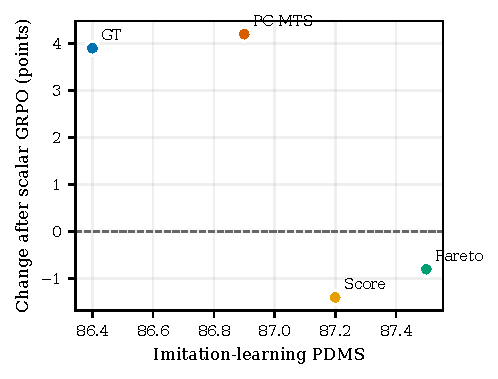
\includegraphics[width=\linewidth]{figures/generated/supervision_mismatch.pdf}
  \caption{Paper-reported imitation PDMS versus the change after the common
  scalar-GRPO stage on NAVSIM v1.  A high imitation score alone does not
  predict optimization value: Score and Pareto regress, whereas PC-MTS gains
  4.2 points.  Each marker is one reported point estimate; the paper does not
  state run/seed aggregation and no synthetic error bars are shown.}
  \label{fig:supervision-mismatch}
\end{figure}

The comparison should be interpreted at the level supported by the evidence.
It demonstrates that a higher-scoring imitation checkpoint need not be a
better starting distribution for GRPO, and that the PC-MTS set is compatible
with a large positive update in this run.  The archived paper table does not
contain scene-level outputs, acceptance counts, or multiple seeds for these
four cells.  Consequently, it does not by itself establish that the reversal
is invariant to seed, nor does it isolate candidate count from the four
filtering decisions.  We therefore do not attach synthetic error bars or
policy-distance values to these points.

\subsection{Candidate-count-matched reconstruction protocol}
\label{sec:pcmts-matched-protocol}

The released reproduction configuration turns the missing causal controls
into a predeclared, low-ambiguity experiment.  All four variants start from the
same GT-only checkpoint, use the same candidate sources, contribute exactly
one target per scene and update, train imitation learning for 200 epochs, and
then run scalar GRPO with 16 rollouts per scene for 10 epochs.  Within each
navigation-command/source stratum, accepted candidates are deterministically
subsampled to the smallest retained count across variants.  The non-GT
sampling probability is held fixed, so a method cannot receive more gradient
updates merely because it retains more candidates.  Empty strata fall back to
the logged trajectory.  In addition to final PDMS, a 300-update diagnostic
records the early GRPO gain before long-horizon training effects can dominate.

For a fully specified reconstruction when the original resolved PC-MTS
manifest is unavailable, the release marks the following as \emph{proposed
reproduction settings}, not measured settings of the reported run: a rollout
bank of 16, $K=3$ neighbors, a command-conditional 0.95 calibration quantile,
and eight temporally correlated local perturbations.  The rollout bank and
calibration queries are disjoint by construction.  Three predeclared training
seeds (20260726, 20260727, and 20260728) are used for the reconstruction, while
bootstrap seed 2027 is reserved for analysis and is never treated as an additional
training run.  These choices fill the executable configuration without
retroactively attributing unrecorded hyperparameters to the main-paper result.

For each run, the pipeline records retained candidates, acceptance rate,
candidate-source composition, feasible rollout rate, feasible high-quality
rate, all-infeasible-group rate, zero-score rate, the 10th percentile,
CVaR-10, 300-update gain, and final scalar-GRPO PDMS.  Method differences are
computed on identical scenes with a 10,000-resample paired bootstrap; means
and standard deviations are reported across the three training seeds.

\subsection{Filter attribution and sensitivity}
\label{sec:pcmts-components}

The component experiment is cumulative: (i) aggregate Score only, (ii) Score
plus the component-wise Pareto gate, (iii) the preceding gates plus calibrated
policy compatibility, and (iv) the full selector with local-feasibility
testing.  Counts are matched after each gate, rather than relaxing a stricter
gate to reach a target count.  This distinction matters: a matched count must
not reintroduce candidates that failed the mechanism being tested.  The
decisive diagnostic is not imitation PDMS alone, but whether adding a gate
raises feasible rollout density and converts the fixed-budget GRPO change from
negative to positive.

The companion sensitivity protocol varies one factor at a time: rollout-bank
size in $\{8,16,32\}$, $K$ in $\{1,3,5\}$, calibration quantile in
$\{0.90,0.95,0.975\}$, and perturbation count in $\{4,8,16\}$.  Compatibility
alternatives are compared at the same acceptance rate: candidate-to-GT
ADE/FDE, distance to the deterministic policy output, minimum rollout-bank
distance, average $K$-nearest distance, and command-calibrated $K$-nearest
distance.  These are evidence-bounded planned analyses: the release contains
their configurations and logging schema, but no unexecuted outcome is used to
support the paper's reported 91.1 PDMS.

Taken together, the existing reversal and the matched protocol close two
different parts of the argument.  The former establishes that isolated target
quality can disagree with downstream optimization value; the latter defines
the experiment needed to attribute that disagreement specifically to policy
compatibility rather than supervision quantity.

  \section{FF-PGRPO Analyses: Feasibility Before Positive Credit}
\label{sec:ffpgrpo-analysis}

Aggregate reward can hide an unsafe trade: progress or comfort may increase
enough to give positive standardized advantage even when collision avoidance,
drivable-area compliance, or a protected reference metric regresses.  The
purpose of FF-PGRPO is therefore not merely to reshape the scalar score, but to
change which rollouts are eligible for positive credit.

\subsection{What the stage ablation establishes}
\label{sec:ffpgrpo-stage-ablation}

On NAVSIM v1, the no-stage baseline in the main ablation has 86.5 PDMS, 98.1
NC, 94.7 DAC, 94.2 TTC, and 80.9 EP.  Applying FF-PGRPO without PC-MTS reaches
91.0 PDMS, with 98.4 NC, 98.0 DAC, 95.8 TTC, and 85.93 EP.  With PC-MTS as the
initialization, FF-PGRPO reaches 91.1 PDMS, 98.5 NC, 98.0 DAC, 96.0 TTC, and
86.0 EP before APR.  The improvement is therefore not produced by sacrificing
the displayed hard-safety components for progress: DAC improves by 3.3 points
and TTC by 1.6 points in the FF-PGRPO-only row, while EP increases by 5.03
points.  These are paper-reported point estimates whose run/seed aggregation
is not stated, so the small 0.1-point
difference between the two FF-PGRPO rows is not presented as a stable gain.

\begin{table*}[t]
\centering
\small
\caption{Stage-wise NAVSIM v1 ablation under single-trajectory inference. Higher is better. Rows are one paper-reported run; only the final AMPT row is independently reproduced from 12,138 scene scores.}
\label{tab:stage_ablation}
\resizebox{\textwidth}{!}{%
\begin{tabular}{lcccccccccccc}
\toprule
configuration & pcmts & scalar\_grpo & ff\_pgrpo & apr & NC & DAC & TTC & C & EP & PDMS & evidence & runs \\
\midrule
GT-only & no & no & no & no & 98.1 & 94.7 & 94.2 & 100.0 & 80.9 & 86.5 & paper reported & 1 reported \\
PC-MTS & yes & no & no & no & 98.2 & 95.2 & 94.5 & 100.0 & 81.3 & 86.9 & paper reported & 1 reported \\
Scalar optimization & no & yes & no & no & 98.4 & 98.0 & 95.8 & 100.0 & 85.93 & 91.0 & paper reported & 1 reported \\
PC-MTS + FF-PGRPO & yes & no & yes & no & 98.5 & 98.0 & 96.0 & 100.0 & 86.0 & 91.1 & paper reported & 1 reported \\
Full AMPT & yes & no & yes & yes & 98.5 & 98.0 & 96.0 & 100.0 & 86.7 & 91.4 & paper reported / final row scene-reproduced & 1 reported + 12138 scenes final \\
\bottomrule
\end{tabular}%
}
\end{table*}


This result is consistent with the proposed ordering---recover feasibility,
then optimize continuous quality---but an aggregate stage ablation cannot
directly reveal the sign of individual rollout credits.  The fixed hard-scene
transition in Section~\ref{sec:hard658} provides scene-level evidence, and the
instrumentation below defines the rollout-level test.

\subsection{Credit diagnostics}
\label{sec:ffpgrpo-credit-diagnostics}

For rollout $i$, let $A_i>0$ denote positive assigned advantage and let
$V_i=1$ denote a violation of any hard-feasibility, protected-reference, or
admissible-Pareto condition.  We report
\begin{equation}
  \mathrm{PCVR} =
  \frac{\sum_i \mathbb{1}[A_i>0]V_i}
       {\sum_i \mathbb{1}[A_i>0]},
  \label{eq:positive-credit-violation}
\end{equation}
and separately count reference-regressing and Pareto-dominated positive
credits.  A denominator of zero is reported as ``no positive credits,'' not as
zero violation.  FF-PGRPO's implementation makes a violating rollout
ineligible for positive credit and exposes assertions for this contract.  The
archived training run, however, does not contain the per-rollout trace needed
to quote an observed PCVR; we do not convert a code invariant into a fabricated
measured rate.

The stepwise mechanism ablation adds: (i) the hard feasibility gate, (ii) the
coherent-reference guard, (iii) the Pareto positive-credit gate, and (iv) the
all-infeasible recovery rule.  Every variant logs group state
(all-feasible/mixed/all-infeasible), feasibility rate, positive and negative
advantage means, PCVR, reference-regressing positive-credit rate,
dominated-positive-credit rate, zero-to-feasible repair, positive-to-zero
regression, and updates until the first feasible rollout.  The coherent
reference is always one executable trajectory.  The historical
component-wise envelope remains only as an ablation because combining the best
value of each metric from different trajectories may describe no realizable
plan and can make every sampled rollout appear to regress.

The low-cost diagnostic run uses the paper's group size of 16 and stops at 300
updates; the final run uses the reported 10 epochs.  All variants share the
same sampled rollout tensors when credit is recomputed offline, which makes
the initial credit-assignment comparison independent of policy drift.  New
training is required only for the subsequent learning curves and remains
disabled unless explicitly enabled.

\subsection{Hard-scene evidence for feasibility-first recovery}
\label{sec:ffpgrpo-hard-evidence}

The manuscript recovery checkpoint is evaluated on the same 658-scene set as
scalar GRPO.  Scalar GRPO produces a positive score in 367 scenes (55.8\%,
95\% Wilson CI 52.0--59.5\%), whereas the AMPT recovery checkpoint is positive
in 440 scenes (66.9\%, CI 63.2--70.4\%).  The comparison uses a single
trajectory per scene and neither method uses test-time sampling, scoring, or
reranking.  Crucially, the paired transition is not merely a difference of
gross counts: 93 scalar-GRPO zeros become positive, 20 scalar-GRPO positives
become zero, 347 successes are retained, and 198 failures persist.  Net
recovery is therefore $93-20=73$ scenes, or 11.1 percentage points.  A
10,000-resample scene-paired bootstrap (analysis seed 2027) gives a 95\% CI of
8.1--14.3 percentage points for this paired change.  This interval quantifies
scene variation for this fixed checkpoint pair; it does not replace missing
multi-seed training uncertainty.

The subset mean PDMS increases from 0.5101 to 0.6145.  The corresponding
component means change from 0.8381 to 0.8815 for NC, 0.7052 to 0.7781 for DAC,
0.7705 to 0.8161 for TTC, and 0.4956 to 0.5932 for EP; comfort increases from
0.9985 to 1.0000, while DDC changes from 0.9567 to 0.9521.  This last decrease
is why protected metrics must be reported next to aggregate recovery rather
than summarized as universal component-wise improvement.  The complete
transition and failure-type decomposition are given in
Section~\ref{sec:hard658}.

The aggregate ablation, paired hard-scene transition, and positive-credit
instrumentation serve complementary roles.  The first shows the overall stage
gain, the second verifies that recovery is net positive rather than purchased
entirely with new failures, and the third is the predeclared test of the
claimed credit-assignment mechanism.

  \section{APR Analyses: Dynamic, Policy-Relative Teachers}
\label{sec:apr-analysis}

APR addresses a moving-target problem.  A trajectory that is a useful local
teacher for the current policy can become redundant after refinement, while a
previously distant candidate can enter the policy's compatible neighborhood.
The relevant question is therefore not whether additional optimization steps
help, but whether rebuilding and re-auditing the teacher set provides useful
targets while retaining already safe behavior.

\subsection{Round-wise behavior and protected components}
\label{sec:apr-rounds}

The main paper reports a monotonic sequence of 91.10, 91.21, 91.37, and 91.45
PDMS from Round 0 through Round 3, corresponding to gains of $+0.11$, $+0.16$,
and $+0.08$.  In the stage ablation, adding APR to the PC-MTS+FF-PGRPO policy
raises PDMS from 91.1 to 91.4 and EP from 86.0 to 86.7, while the displayed NC,
DAC, TTC, and comfort values remain 98.5, 98.0, 96.0, and 100, respectively.
This pattern is aligned with APR's design: local teacher updates increase
progress without visible regression in the protected components at the
reported precision.

Each round value is a reported checkpoint summary; its run/seed aggregation is
not stated.  No across-seed
standard deviation is available, and the 0.08--0.16 point increments are not
claimed to be independently significant.  Moreover, the archived experiment
history contains accepted and rejected branches rather than a single complete
three-round hash chain; the four values above are therefore treated as the
paper's round-level summary, not as permission to infer missing intermediate
measurements.

\begin{table}[t]
\centering
\small
\caption{Paper-reported NAVSIM v1 APR progression under single-trajectory inference. Higher is better. Run/seed aggregation is not stated and no training-seed confidence interval is available.}
\label{tab:apr_rounds}
\resizebox{\linewidth}{!}{%
\begin{tabular}{lcccc}
\toprule
round & pdms & gain\_points & evidence & runs \\
\midrule
0 & 91.1 & 0.0 & paper reported & reported point; run/seed aggregation not stated \\
1 & 91.21 & 0.11 & paper reported & reported point; run/seed aggregation not stated \\
2 & 91.37 & 0.16 & paper reported & reported point; run/seed aggregation not stated \\
3 & 91.45 & 0.08 & paper reported / final score scene-reproduced & reported point + 12138 final scenes; run aggregation not stated \\
\bottomrule
\end{tabular}%
}
\end{table}


\begin{figure}[t]
  \centering
  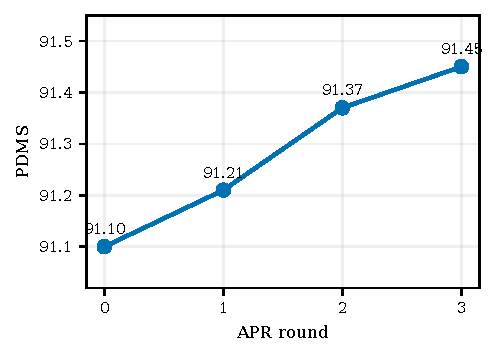
\includegraphics[width=\linewidth]{figures/generated/apr_rounds.pdf}
  \caption{Paper-reported NAVSIM v1 progression across APR rounds.  The final
  point is reproduced at scene level, but the small round increments are from
  one reported sequence and carry no across-seed error bar.}
  \label{fig:apr-rounds}
\end{figure}

\subsection{Teacher audit and post-interpolation evaluation}
\label{sec:apr-teacher-audit}

One traceable APR teacher-construction pass starts from 39,261 strict external
trajectories: 25,402 (64.7\%) from one driving-policy source and 13,859
(35.3\%) from a second source.  After interpolation with coefficient 0.25 and
exact re-evaluation, 28,910 targets remain, an acceptance rate of 73.6\%; the
remaining 10,351 are rejected.  These counts are from one audited navtrain
construction pass and are not presented as the source proportions of every
APR round.  They nevertheless establish an important operational fact:
interpolation is followed by evaluator-based admission, and the check is
non-vacuous---more than one quarter of the pre-audit union does not enter the
distillation set.

\begin{table}[t]
\centering
\small
\caption{Audited APR teacher-pool construction on NAVSIM navtrain. Counts are from one archived teacher audit; the 28,910 accepted teachers follow interpolation and exact re-evaluation. Higher acceptance is not inherently better because guards constrain quality.}
\label{tab:apr_teacher_pool}
\resizebox{\linewidth}{!}{%
\begin{tabular}{lcccc}
\toprule
step & source & count & acceptance\_definition & evidence \\
\midrule
source selection & DriVor & 25402 & source-specific strict candidates & archived APR runbook \\
source selection & DiffusionDriveV2 & 13859 & source-specific strict candidates & archived APR runbook \\
strict union & merged sources & 39261 & feasible and component-protected before interpolation & deterministic sum of audited source counts \\
post-interpolation audit & accepted teachers & 28910 & alpha 0.25 then exact re-evaluation & archived APR runbook \\
\bottomrule
\end{tabular}%
}
\end{table}


Teacher status is defined relative to the current policy.  A candidate is
\emph{accepted} when its evaluated local target is feasible, exceeds the
current single prediction by the required margin, preserves protected
metrics, and stays inside the current rollout neighborhood.  An accepted
teacher becomes \emph{expired} if it fails those tests after the policy is
updated.  A previously rejected candidate is \emph{newly activated} if it
passes after the rollout bank and current prediction are regenerated.  These
definitions prevent lifecycle counts from being conflated with raw pool size.

The interpolation search is descending: larger moves are evaluated first and
the first admissible move is retained.  Every accepted target stores the
teacher, current prediction, interpolation coefficient, post-interpolation
score, protected-metric deltas, compatibility distance, and evaluator hash.
No-interpolation and no-post-evaluation controls remove different safeguards:
the former jumps directly to the teacher, whereas the latter retains a local
trajectory without verifying that interpolation preserved feasibility.

\subsection{Step-matched controls}
\label{sec:apr-controls}

The release defines eight variants from the same Round-0 checkpoint and
matches the total number of optimizer updates: extra training on the existing
mixture, one-shot distillation, repeated use of a fixed teacher set, dynamic
teachers, dynamic teachers without interpolation, without post-interpolation
re-evaluation, without policy retention, and full APR.  The dynamic-teacher
and full-APR variants rebuild predictions, rollout banks, and teacher audits at
the same three round boundaries reported in the paper.  The fixed-teacher
variant repeats the Round-1 set without re-ranking it; the extra-training
control receives the same update count but no new teacher target.  This design
separates four possible explanations: more updates, teacher supervision in
general, teacher-set rebuilding, and the interpolation/retention safeguards.

For every round, the required report contains PDMS and all components,
regressed scenes, new failures, accepted/expired/newly activated teachers,
mean and median verified teacher advantage, interpolation-coefficient
distribution, and scene coverage.  A checkpoint is promoted only if its
single-trajectory aggregate score improves and protected metrics pass the
same non-regression audit; otherwise the previous checkpoint remains the
dynamic anchor.  Training ends after three promoted rounds or when no audited
local target remains.  These controls are configured but not represented as
measured results in this supplement, because running them would require new
training.

Optional task-vector consolidation is kept separate from teacher discovery.
The implementation can mask low-salience coordinates, require directional
agreement, bound each branch norm and the total displacement from the current
anchor, and then evaluate the merged checkpoint.  The best-branch, simple
average, task-arithmetic, and TIES-style controls are required before assigning
an independent gain to merging~\cite{taskarithmetic2023,ties2023}.  In the
absence of a stable, step-matched gain, merging should be read as a conservative
checkpoint-consolidation detail, not as the source of APR's teacher lifecycle.

The present evidence therefore supports two bounded statements: the reported
APR rounds are monotonic and preserve the displayed safety/compliance metrics,
and an audited construction pass materially filters proposed local targets
after re-evaluation.  The step-matched variants above are the necessary test
for the stronger causal claim that dynamic rebuilding, rather than additional
training alone, explains the full increment.

\begin{table}[t]
\centering
\small
\caption{APR fixed-teacher diagnostic on NAVSIM v1. The archived fixed-set continuation decreases from its 91.2766 anchor, whereas the 91.45 endpoint is the paper's compressed dynamic-round report; the rows are diagnostic rather than a step-matched causal ablation.}
\label{tab:apr_fixed_teacher}
\resizebox{\linewidth}{!}{%
\begin{tabular}{lccc}
\toprule
policy\_or\_epoch & pdms & interpretation & evidence \\
\midrule
dynamic-teacher anchor & 91.2766 & accepted dynamic-teacher checkpoint & archived APR runbook \\
fixed-set continuation epoch 0 & 91.2526 & below dynamic-teacher anchor & archived APR runbook \\
fixed-set continuation epoch 1 & 91.2311 & further below dynamic-teacher anchor & archived APR runbook \\
paper APR round 3 & 91.45 & compressed round-level paper report & paper reported \\
\bottomrule
\end{tabular}%
}
\end{table}


  \section{Failure Recovery and Qualitative Diagnostics}
\label{sec:failure-qualitative}

Qualitative evidence is most useful when organized by a mechanism and tied to
scene-level metrics.  We therefore analyze the fixed hard set first, then give
traceable examples of recovered, persistent, and newly introduced failures.
All quantitative hard-set results and the mechanism-organized case table use
the same historical checkpoint pair as the main paper's 367-versus-440
recovery claim.  The final full-benchmark visualization is separately labeled
and is not used in the 658-scene recovery analysis.

\subsection{Construction of the fixed 658-scene set}
\label{sec:hard658}

The set contains 658 NAVSIM v1 scenes for which the initial ReCogDrive policy
obtained exactly zero PDMS in all five construction samples because of an
at-fault collision (NC), drivable-area violation (DAC), or both.  The set is
fixed before comparing the scalar-GRPO and AMPT recovery checkpoints.  Under
single-trajectory evaluation, scalar GRPO is positive on 367 and zero on 291
scenes; the AMPT recovery checkpoint is positive on 440 and zero on 218.

The paired $2\times2$ transition is
\begin{equation}
\begin{array}{c|cc|c}
 & \multicolumn{2}{c|}{\text{AMPT recovery checkpoint}} & \\
\text{scalar GRPO} & \text{zero} & \text{positive} & \text{row total} \\
\hline
\text{zero}     & 198 & 93  & 291 \\
\text{positive} & 20  & 347 & 367 \\
\hline
\text{column total} & 218 & 440 & 658
\end{array}.
\label{eq:hard658-transition}
\end{equation}
Hence 93 failures are repaired, 347 successes are retained, 198 failures
persist, and 20 new failures appear.  The net change is $93-20=73$, exactly the
difference between the gross positive counts $440-367$.  This distinction is
important: 440/658 is the gross recovery rate relative to the policy used to
construct the hard set, whereas 93 and 20 describe the paired transition from
scalar GRPO to the AMPT recovery checkpoint.  The resulting 11.1-percentage-
point paired improvement has a scene-bootstrap 95\% CI of 8.1--14.3 points
(10,000 resamples, seed 2027).  It is a net improvement rather than an exchange
of an equal number of old and new failures.

\begin{table}[t]
\centering
\small
\caption{Recovery on the same 658 NAVSIM v1 scenes under one archived comparison. Rates use Wilson 95\% intervals over scenes; this interval does not represent training-seed uncertainty. Higher recovery is better.}
\label{tab:failure_recovery}
\resizebox{\linewidth}{!}{%
\begin{tabular}{lcccccc}
\toprule
Method & Positive & Zero & Recovery rate (\%) & Wilson 95\% CI (\%) & Runs & Scenes \\
\midrule
Scalar GRPO & 367 & 291 & 55.8 & [52.0, 59.5] & 1 archived comparison & 658 \\
AMPT recovery checkpoint & 440 & 218 & 66.9 & [63.2, 70.4] & 1 archived comparison & 658 \\
\bottomrule
\end{tabular}%
}
\end{table}

\begin{table}[t]
\centering
\small
\caption{Paired recovery change on 658 NAVSIM v1 scenes. The 11.1-point gain has a scene-paired bootstrap interval (10,000 resamples, analysis seed 2027); higher net repair is better. One archived model pair is available.}
\label{tab:failure_net_gain}
\resizebox{\linewidth}{!}{%
\begin{tabular}{lcccccc}
\toprule
Absolute gain (pp) & Paired 95\% CI (pp) & Zero-to-positive & Positive-to-zero & Net repair & Scenes & Runs \\
\midrule
11.1 & [8.1, 14.3] & 93 & 20 & 73 & 658 & 1 archived comparison \\
\bottomrule
\end{tabular}%
}
\end{table}


\begin{figure}[t]
  \centering
  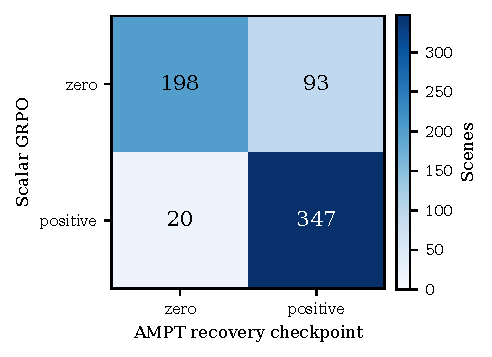
\includegraphics[width=\linewidth]{figures/generated/failure_transition.pdf}
  \caption{Scalar-GRPO to AMPT transition on the fixed 658-scene set.  The
  off-diagonal cells expose both 93 repairs and 20 regressions, rather than
  reporting gross recovery alone.}
  \label{fig:failure-transition}
\end{figure}

The original hard-set taxonomy contains 480 DAC-only scenes, 165 collision-
only scenes, 13 scenes failing both, and no residual ``other'' category.  The
paired repairs/new failures are 59/14 for DAC-only, 32/6 for collision-only,
and 2/0 for the joint category, giving net changes of 45, 26, and 2 scenes.
The gains are therefore not concentrated in only one failure type, although
the small joint category is descriptive rather than statistically decisive.

\begin{table}[t]
\centering
\small
\caption{Failure-type decomposition for the fixed 658 NAVSIM v1 scenes. Repairs and regressions use the scalar-GRPO to AMPT transition; net repairs sum to 73. One archived comparison; higher net repair is better.}
\label{tab:failure_causes}
\resizebox{\linewidth}{!}{%
\begin{tabular}{lcccc}
\toprule
Failure type & Scenes & Repairs & Regressions & Net repair \\
\midrule
DAC-only/all-fail & 480 & 59 & 14 & 45 \\
collision-only/all-fail & 165 & 32 & 6 & 26 \\
collision + DAC & 13 & 2 & 0 & 2 \\
\bottomrule
\end{tabular}%
}
\end{table}


\begin{figure}[t]
  \centering
  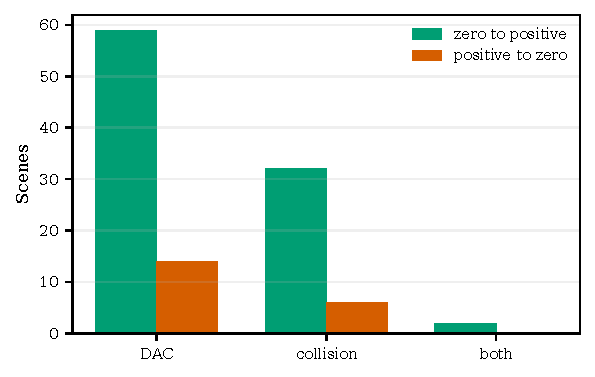
\includegraphics[width=\linewidth]{figures/generated/failure_cause_recovery.pdf}
  \caption{Repairs and regressions by the fixed hard-set cause taxonomy.  The
  net changes are 45 DAC, 26 collision, and 2 joint cases, totaling 73.}
  \label{fig:failure-causes}
\end{figure}

\subsection{Traceable scene cases}
\label{sec:traceable-cases}

Table~\ref{tab:hard658-cases} selects cases by transition type, not by visual
appeal.  Navigation commands come from the corresponding NAVSIM scene
metadata; scores and components come from the fixed paired evaluation.  The
table uses full scene identifiers so every row can be regenerated.  Component
pairs are scalar-GRPO $\rightarrow$ AMPT-recovery values.

\begin{table*}[t]
\centering
\small
\caption{Mechanism-organized examples from the fixed 658-scene set. Scene IDs and PDMS values are reproduced from the archived comparison; commands are joined from audited scene metadata. These selected cases are not an unbiased benchmark sample.}
\label{tab:hard658-cases}
\resizebox{\textwidth}{!}{%
\begin{tabular}{lccccccccc}
\toprule
Scene ID & Command & Outcome & PDMS & NC & DAC & TTC & EP & DDC & Diagnosis \\
\midrule
00fcad6d092c5e8e & left & repaired & 0.000 -> 1.000 & 0.000 -> 1.000 & 1.000 -> 1.000 & 0.000 -> 1.000 & 0.000 -> 1.000 & 1.000 -> 1.000 & Collision/TTC failure repaired without protected regression. \\
03aa8a0576a25b63 & right & repaired & 0.000 -> 0.963 & 1.000 -> 1.000 & 0.000 -> 1.000 & 1.000 -> 1.000 & 0.000 -> 0.912 & 1.000 -> 1.000 & Drivable-area failure repaired while NC and TTC remain feasible. \\
1148c72f141c532d & left & partial repair & 0.000 -> 0.583 & 0.000 -> 1.000 & 0.000 -> 1.000 & 0.000 -> 0.000 & 0.000 -> 1.000 & 1.000 -> 1.000 & Both hard failures repaired; TTC remains the limiting component. \\
00016f8b45c25a1d & left & persistent & 0.000 -> 0.000 & 1.000 -> 1.000 & 0.000 -> 0.000 & 1.000 -> 1.000 & 0.000 -> 0.000 & 0.000 -> 0.000 & DAC/progress failure persists under both audited checkpoints. \\
4b4a268bee4c5ab5 & left & regressed & 1.000 -> 0.000 & 1.000 -> 1.000 & 1.000 -> 0.000 & 1.000 -> 1.000 & 1.000 -> 0.000 & 1.000 -> 1.000 & A DAC regression creates a new zero and motivates retention. \\
\bottomrule
\end{tabular}%
}
\end{table*}


The first two cases are consistent with feasibility-oriented recovery: a hard
component changes from zero to one and positive PDMS returns.  Scene-level
before/after metrics do not identify the temporal order of training updates.
The third shows why ``recovered'' does not mean component-wise perfect.  The
fourth remains a DAC/progress failure under both audited checkpoints; without a
candidate/rollout manifest, the metrics do not identify whether pool coverage,
policy support, or optimization is responsible.  The fifth prevents
survivorship bias in the qualitative analysis and
motivates APR retention; it is one of the 20 positive-to-zero transitions
already charged against net recovery.

\subsection{Mechanism-centered visualization protocol}
\label{sec:qualitative-protocol}

The supplied renderer groups panels by decision rather than by scene
similarity.  A PC-MTS panel overlays an accepted candidate, a rejected distant
candidate, the logged trajectory, and the frozen-policy rollout neighborhood.
An FF-PGRPO mixed-group panel distinguishes unsafe, feasible-but-dominated,
and admissible Pareto-positive rollouts and prints their assigned advantages;
an all-infeasible panel shows the coherent recovery reference.  An APR panel
shows the current prediction, raw teacher, evaluated interpolant, and the
accepted/expired/newly-activated lifecycle state.  Every rendered panel reads
the scene id, command, component scores, and method name from its manifest and
uses a common legend: blue for the current prediction, green for an accepted
or positively credited trajectory, orange for a dominated/expired trajectory,
red for an unsafe trajectory, and black dashed for the coherent reference.

This protocol is also a safeguard against overinterpretation.  A camera/BEV
image is emitted only when the frame, command, all trajectories, and evaluator
record share the same scene identifier.  The metric-only cases in
Table~\ref{tab:hard658-cases} remain quantitative case studies if those visual
assets are unavailable; no unrelated camera frame or hand-drawn trajectory is
substituted merely to complete a panel.

\begin{figure*}[t]
  \centering
  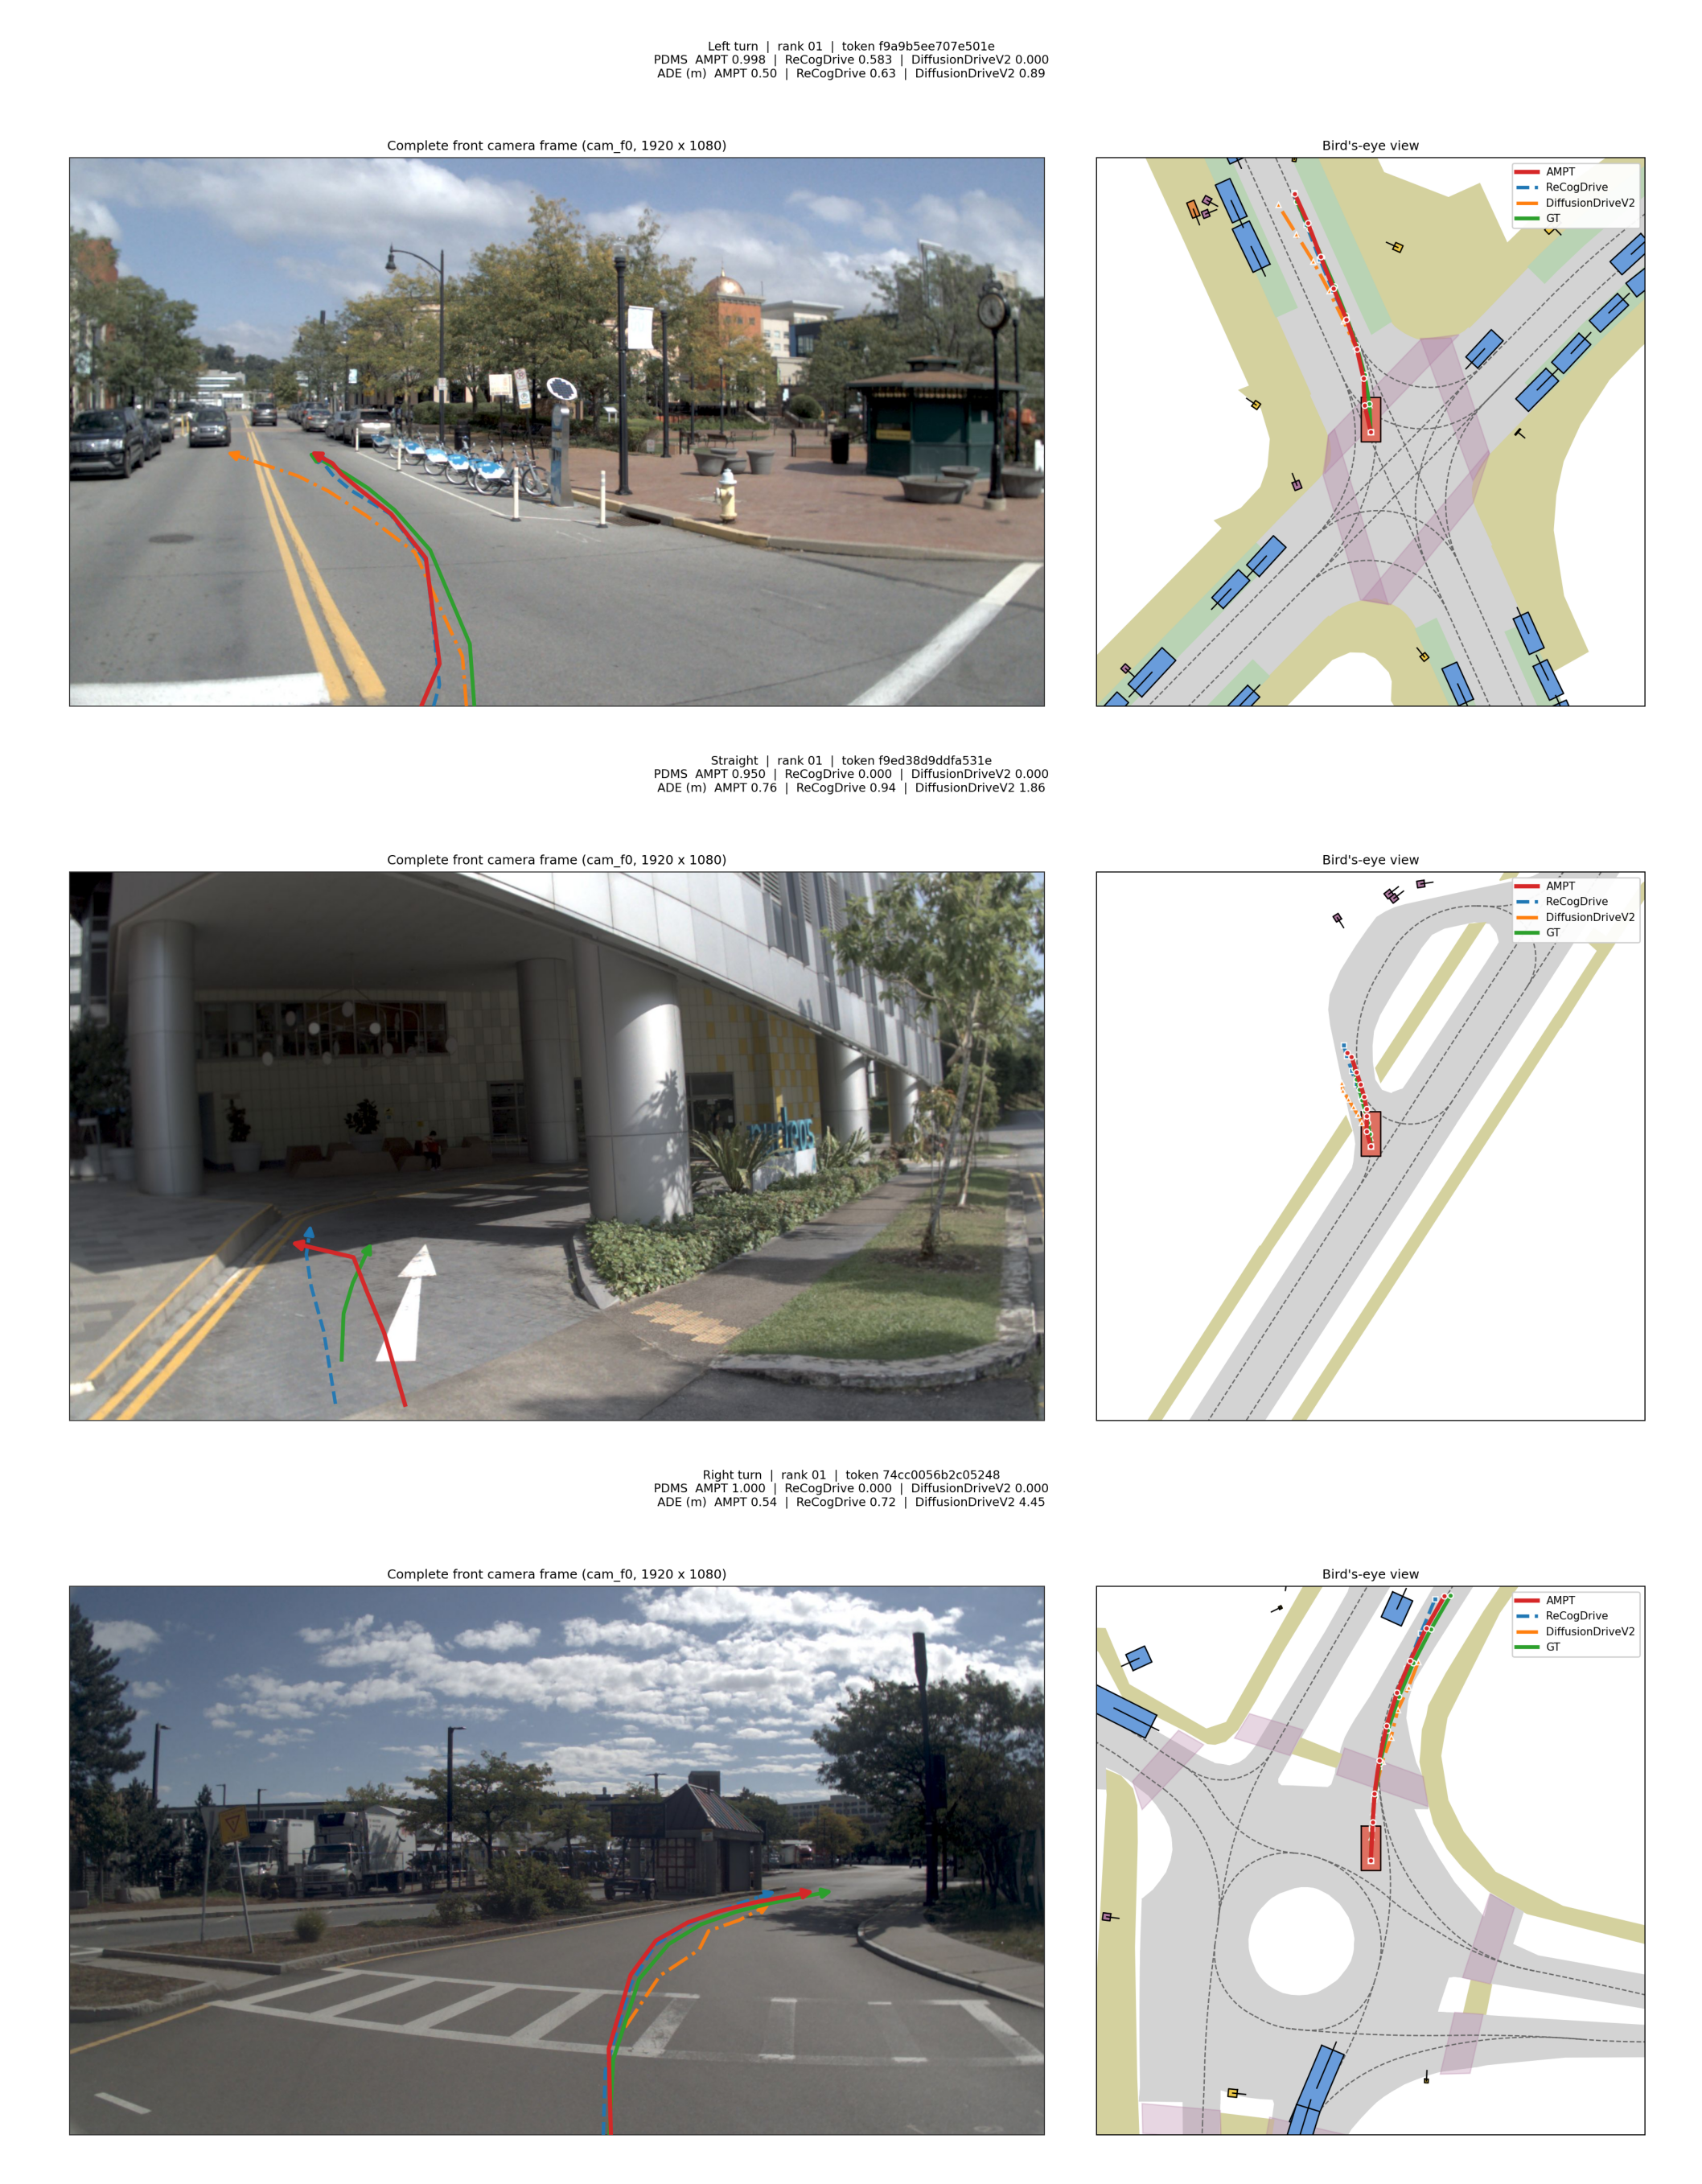
\includegraphics[width=0.92\textwidth]{figures/generated/qualitative_selected_cases.png}
  \caption{Three selected full-benchmark NAVSIM v1 cases (left, straight, and
  right commands) rendered from the separately audited final-AMPT manifest.
  Each row contains the complete front frame, bird's-eye view, scene ID,
  command, color legend, PDMS, and trajectory error.  These examples are not
  members of, and contribute no statistics to, the historical 658-scene
  recovery comparison; they illustrate final-policy behavior only.}
  \label{fig:qualitative-selected}
\end{figure*}

\clearpage

  \section{Additional Related Work, Fair Comparison, and Limitations}
\label{sec:related-limitations}

\subsection{Related perspectives}

\textbf{Support-aware policy improvement.}
Conservative offline policy-improvement methods limit updates in regions where
the behavior data provide weak support.  SPIBB constrains uncertain decisions
to the baseline policy~\cite{spibb2019}, while BEAR regularizes a learned policy
toward the behavior distribution~\cite{bear2019}.  PC-MTS shares the support
intuition but applies it before optimization: it filters trajectory-level
supervision using samples from the frozen learner, with command-conditional
calibration and a local feasibility test.  It is not a general monotonic-
improvement guarantee; its role is to avoid moving the imitation policy into a
region where downstream rollout optimization has poor local support.

\textbf{Multi-objective and Pareto optimization.}
Multi-objective reinforcement learning studies policies under vector-valued
returns and alternative preference models~\cite{roijers2013}.  AMPT does not
seek a global set of Pareto-optimal policies.  PC-MTS uses a scene-local Pareto
filter for supervision, and FF-PGRPO uses a hierarchy: hard feasibility and
coherent-reference guards are evaluated before a rollout can receive positive
Pareto credit.  This order is essential when an aggregate score can compensate
for a protected regression.

\textbf{Advantage-weighted behavior learning.}
Advantage-weighted regression turns estimated advantages into weights for
supervised policy updates~\cite{awr2021}.  APR is related at the loss level,
but its weights are attached only after a candidate is compared with the
current single-trajectory prediction, locally interpolated, and re-evaluated.
Teacher admission and policy retention are therefore as important as the
weighting function itself.

\textbf{Model merging.}
Task arithmetic combines model displacements relative to a shared
anchor~\cite{taskarithmetic2023}, and TIES resolves redundancy and sign
conflicts before merging~\cite{ties2023}.  AMPT may use an anchor-constrained
variant to consolidate APR branches, but merging is optional and is separated
from teacher selection.  Passing parameter-space norm and sign checks does not
imply behavioral safety; every merged checkpoint must still undergo the same
single-trajectory evaluator audit.

\subsection{Fair-comparison boundary}
\label{sec:fair-comparison}

AMPT uses one predicted trajectory at inference.  Policy rollout banks,
candidate pools, coherent references, group sampling, specialist policies, and
the offline evaluator are training-only; there is no test-time scorer,
best-of-$N$ selection, or candidate reranking.  This contract is present in the
paper and is independently supported by the v1 submission provenance.

The released v1 scene export contains 12,138 successfully scored scenes from
12,146 predictions; the eight unscored predictions are disclosed rather than
imputed.  The v2 export contains 12,146 successful scene scores.  Its EC
aggregation follows the official evaluator, although a direct EC value is
present for 10,040 rows.  Scene-bootstrap intervals resample these scored
scenes and are explicitly labeled as scene uncertainty; they are not a
substitute for independent training runs.

The baseline rows in the main tables are treated as \emph{reported} unless a
local scene export and matching protocol are available.  AMPT's v1/v2 rows are
reproduced from scene-level outputs, but protocol matching is not established
for every external baseline.  Moreover, the audited v1 provenance records use
of navtest for checkpoint selection.  We therefore avoid a strict held-out
state-of-the-art claim and report protocol fields---backbone, sensors, training
data, inference candidates, and test-time scoring---alongside each comparison.

The 658-scene result uses the recovery checkpoint and checkpoint pair specified
by the main-paper analysis.  It is a fixed-subset diagnostic, not a claim that
every later checkpoint must induce the same transitions.  Reporting the full
$2\times2$ matrix in Eq.~\ref{eq:hard658-transition} makes the gross and net
notions of recovery explicit.

\subsection{Limitations}
\label{sec:limitations}

\textbf{Finite support estimates.}
Compatibility is estimated from a finite rollout bank.  Sparse commands or
multi-modal scenes can make a genuinely useful target appear distant, and the
calibrated neighborhood is only as representative as the frozen policy
samples.  Increasing bank size improves coverage but raises offline inference
and storage cost.

\textbf{Evaluator bias and non-reactive evaluation.}
All three stages use an offline NAVSIM evaluator for filtering, credit, or
teacher validation.  Systematic evaluator errors can therefore be amplified
across stages.  NAVSIM's non-reactive agents also cannot reveal how other road
users would respond to the learned trajectory; feasibility under this scorer
is not a closed-loop safety guarantee.

\textbf{Candidate-pool ceiling.}
APR can select and localize only behaviors represented in its multi-source
pool.  If no source proposes a valid maneuver, rebuilding the pool changes no
target.  The persistent case in Table~\ref{tab:hard658-cases} establishes
persistence under two audited checkpoints, but cannot diagnose this pool
ceiling without a per-scene candidate manifest.

\textbf{Locality can reject long-horizon value.}
The policy-compatibility filter intentionally favors learnable local targets.
It may reject a distant behavior that is initially difficult to imitate but
would be valuable after a longer curriculum.  Policy-dependent teacher-value
and cross-policy selection experiments are therefore important follow-ups.

\textbf{Benchmark-specific hierarchy.}
The ordering of NC/DAC feasibility, DDC/TLC guards, progress floors, and
continuous Pareto objectives reflects NAVSIM metrics.  Transferring AMPT to a
new benchmark requires revalidating the hierarchy and calibration thresholds,
not merely renaming metric fields.

\textbf{No behavioral semantics for parameter merging.}
Task-vector masks, direction agreement, and norm constraints bound parameter
movement but do not provide a semantic or safety guarantee.  If its independent
gain is not stable across seeds and step-matched controls, merging should
remain an implementation detail.

\textbf{Statistical scope.}
The supervision comparison, stage ablation, and APR round table are available
as reported point estimates rather than three-seed aggregates.  Small APR
increments must not be described as stable until the configured multi-seed
controls are run.  The paired 658-scene interval establishes a robust scene-
level net transition for one checkpoint pair, but does not measure training-
seed variation.

These limitations narrow rather than alter the paper's central claim.  The
currently traceable evidence establishes the supervision--optimization
reversal, a large feasibility-oriented stage gain, monotonic reported APR
rounds with preserved displayed safety components, and positive net recovery
on a fixed hard set.  Candidate-count matching, rollout-level credit traces,
step-matched APR controls, and multi-seed reruns are the remaining experiments
needed for stronger causal and stability claims.

  \expandafter\endinput
\fi

\documentclass[10pt,twocolumn]{article}
\usepackage[letterpaper,margin=0.72in]{geometry}
\usepackage[T1]{fontenc}
\usepackage{lmodern}
\usepackage{microtype}
\usepackage{amsmath,amssymb}
\usepackage{booktabs}
\usepackage{graphicx}
\usepackage{xcolor}
\usepackage{url}
\usepackage[hidelinks]{hyperref}
\setlength{\columnsep}{0.22in}
\setlength{\textfloatsep}{7pt plus 2pt minus 2pt}
\setlength{\floatsep}{6pt plus 2pt minus 2pt}
\setlength{\intextsep}{6pt plus 2pt minus 2pt}

\newcommand{\method}{AMPT}
\newcommand{\pc}{PC-MTS}
\newcommand{\ff}{FF-PGRPO}
\newcommand{\apr}{APR}
\newcommand{\reported}{\textsuperscript{R}}
\newcommand{\reproduced}{\textsuperscript{S}}
\newcommand{\proposed}{\textsuperscript{P}}

\title{Supplementary Material for\\
\textit{Aligning Multi-Trajectory Supervision with Policy Optimization for VLA Driving}}
\author{Anonymous Submission}
\date{}

\begin{document}
\maketitle
\begin{abstract}
This supplement specifies the three stages of Aligned Multi-Trajectory Policy
Training (AMPT), records implementation and evaluation provenance, and expands
the supervision, credit-assignment, policy-refinement, and failure-recovery
analyses.  Superscripts R, S, and P denote paper-reported, scene-level
reproduced, and proposed-but-unrun reproduction settings, respectively.  This
distinction prevents a proposed control from being mistaken for an observed
result.  Unless stated otherwise, evaluation emits one trajectory and performs
neither test-time scoring nor candidate reranking.
\end{abstract}

\appendix
\section{Additional Method Details}
\label{sec:additional-method}

This appendix makes explicit the contracts that connect the three training
stages.  This is important because the central claim of AMPT is not that a
trajectory with a high offline score is automatically a useful target, but
that supervision, rollout credit, and policy-relative refinement must agree on
what the current policy can safely learn.  We use three provenance labels
throughout.  \emph{Paper-reported} denotes a value stated in the main paper,
\emph{scene-level reproduced} denotes a value recomputed from an archived
per-scene evaluator export, and \emph{proposed reproduction} denotes a fully
specified setting for rerunning an experiment whose resolved training manifest
was not retained.  The last category is a protocol, not an observed result.

\subsection{Policy-Compatible Multi-Trajectory Supervision}
\label{sec:pc-mts-details}

\paragraph{Candidate construction and source balancing.}
For a scene $s$, let $\tau_s^0$ be the logged trajectory and let
$\mathcal C_s=\cup_m\mathcal C_s^{(m)}$ be the union of candidates supplied by
the configured proposal generators.  PC-MTS is source agnostic: a source may
be another policy seed, a structured trajectory expander, or a specialist
planner, but source identity is retained in the manifest and geometric near-
duplicates are merged before scoring.  The logged target is immutable and
is never removed.  A final Stage-1 source-count manifest was not found.  To
make the controlled reconstruction executable without presenting invented
counts as measurements, our \emph{proposed reproduction} caps every non-GT
source at eight candidates per scene before filtering.  When comparing Score,
Pareto, and PC-MTS, we use the same source
cap and retain the same number of non-GT candidates by taking the best valid
items under the corresponding rule.  Thus a difference cannot be attributed
to exposing one variant to a larger target set.

\begin{table*}[t]
\centering
\small
\caption{Candidate-source and audit budgets for PC-MTS on the NAVSIM training universe. Counts tagged proposed are reproduction settings rather than observations; higher/lower is not applicable.}
\label{tab:candidate_sources}
\resizebox{\textwidth}{!}{%
\begin{tabular}{lccccc}
\toprule
source & role & per\_scene\_budget & scene\_universe & retention\_or\_use & status \\
\midrule
Logged trajectory & immutable fallback and retention target & 1 & 103,288 expected navtrain scenes & always retained & paper-described / historical contract \\
Frozen-policy rollout bank & compatibility support estimate & 16 & 103,288-scene reproduction universe & distance calibration only & proposed reproduction setting \\
Multi-source candidate proposals & quality and Pareto targets & 8 per source & 103,288-scene reproduction universe & subject to quality/Pareto/compatibility gates & proposed reproduction budget \\
Correlated local perturbations & local feasibility audit & 8 per retained proposal & same candidate scenes & pass-rate threshold 0.75 & proposed reproduction setting \\
\bottomrule
\end{tabular}%
}
\end{table*}


\paragraph{Quality, feasibility, and Pareto filtering.}
Every complete trajectory is scored by the same offline evaluator used for
training diagnostics.  We first require hard feasibility, then a sufficient
aggregate score, and only then form the scene-wise component Pareto front.  A
candidate $a$ dominates $b$ only if it is no worse on every active Pareto
objective and is strictly better on at least one.  This order matters: a high
progress value cannot compensate for collision or leaving the drivable area.
The paper does not archive the numerical Stage-1 aggregate cutoff.  In the
\emph{proposed reproduction}, a training-split quantile is selected once so
that comparison variants are matched to the minimum retained count, followed
by a source-balanced top-$k$ tie break.  The sealed cutoff is applied
identically to all splits and is never used to synthesize a reported score.

The benchmark-specific partition is summarized below.  On NAVSIM v1, NC and
DAC are hard gates; DDC is protected; and EP, TTC, and comfort are optimized
inside the admissible region.  On NAVSIM v2, NC, DAC, DDC, and TLC are the
multiplicative compliance gates.  The historical metric adapter uses EP, TTC,
and a composite $Q=(\mathrm{LK}+\mathrm{HC}+\mathrm{EC})/3$ as its three
continuous Pareto axes; the official EPDMS report still exposes LK, HC, and EC
separately.  For binary scorer outputs the \emph{proposed reproduction}
requires a value of one up to $10^{-6}$.  The archived safety contract uses
reference-relative tolerances of $0.01$ for DDC/comfort and $0.02$ for TTC/EP;
TLC remains a hard v2 gate.  These are historical implementation values, not a
claim about the unresolved configuration of the paper checkpoint.

\begin{table}[t]
\centering
\small
\caption{NAVSIM v1/v2 metric partition used by PC-MTS and FF-PGRPO. Hard feasibility is tested before protected non-regression and Pareto quality.}
\label{tab:metric_partition}
\resizebox{\linewidth}{!}{%
\begin{tabular}{lcccc}
\toprule
benchmark & hard\_feasibility & protected\_guards & pareto\_quality & aggregate \\
\midrule
NAVSIM v1 & NC, DAC & DDC; non-regression in TTC and feasibility & EP, TTC, C & PDMS \\
NAVSIM v2 & NC, DAC, DDC, TLC & DDC/TLC feasibility; non-regression in TTC & EP, TTC, LK, HC, EC & EPDMS \\
\bottomrule
\end{tabular}%
}
\end{table}


\paragraph{Policy compatibility.}
Let $\mathcal R_s=\{\rho_j\}_{j=1}^{M}$ be rollouts sampled from the frozen
GT-only policy under the same command as the candidate.  We standardize
waypoint displacement with per-timestep, command-conditioned robust scales
fitted on the calibration split, and write the resulting trajectory distance
as $d(\tau,\rho)$.  The archived implementation additionally exposes final
displacement, heading, and velocity diagnostics, but the proposed controlled
comparison changes only the normalized waypoint statistic.  The compatibility
statistic is
\begin{equation}
 d_{\mathrm{PC}}(\tau,\mathcal R_s)
 =\frac{1}{K}\sum_{\rho\in\operatorname{NN}_{K}(\tau;\mathcal R_s)}
 d(\tau,\rho).
\end{equation}
The threshold $q_c$ is the command-specific quantile of leave-one-out policy
rollout distances on calibration scenes.  The archived code proves
leave-one-out calibration within each policy cloud, but its retained manifest
does not prove driving-log-level independence.  The proposed reconstruction
therefore enforces log-disjoint calibration and query scenes.  The paper states the general
$K$-nearest statistic but does not report $M$, $K$, or $q_c$.  The archived
implementation realizes the valid $K=1$ special case.  Our \emph{proposed
reproduction} uses $M=16$, $K=3$, and $q_c$ at the 95th percentile, with
command groups merged into a global fallback only when a command group has
fewer than 16 calibration observations.  This choice is also the center point
of the supplied sensitivity grid, rather than a retrospectively selected
result.

\paragraph{Local feasibility tube.}
Compatibility to one rollout neighborhood does not by itself establish that a
target is robust to small prediction errors.  For every candidate that passes
the previous gates, PC-MTS adds correlated perturbations to $(x,y,\psi)$ and
the implied velocity sequence.  The perturbations are sampled from normalized
policy residuals, smoothed over time, and projected back to the command-consistent
trajectory representation before exact re-evaluation.  This changes whole
trajectory segments rather than independently jittering waypoints.  The
archived implementation supports 16 or 32 perturbations; the \emph{proposed
reproduction} uses eight lower-cost perturbations, preserves the empirical
temporal covariance of policy residuals, and accepts a candidate when at least
six of eight perturbations pass
the hard feasibility gates and the protected guards.  The P1 configuration
evaluates 4/8/16 perturbations and does not tune the threshold on the test
split.

\paragraph{Target sampling and fallback.}
After filtering, the training set for scene $s$ is
$\mathcal T_s=\{\tau_s^0\}\cup\mathcal A_s$, where $\mathcal A_s$ contains
accepted candidates.  A training update draws exactly one target for the
scene, so scenes with many proposals do not receive larger gradients.  The
\emph{proposed reproduction} draws the logged target with probability $0.5$
and otherwise samples uniformly from $\mathcal A_s$; if $\mathcal A_s$ is
empty, it deterministically uses $\tau_s^0$.  Candidate identity is sampled
before the diffusion timestep, so all noisy versions in that update correspond
to a single coherent target.  Fine-tuning uses the same denoising objective as
GT-only training and produces $\pi_{\mathrm{initial}}$.

\paragraph{Implementation correspondence.}
The source-balanced builder and immutable-GT path are implemented at
\path{41a8613:navsim/agents/recogdrive/curriculum/builder.py}
and \path{41a8613:navsim/agents/recogdrive/curriculum/proposals.py}.
Physical distance and calibrated reachability are at
\path{41a8613:navsim/agents/recogdrive/curriculum/reachability.py};
the feasibility and correlated-perturbation checks are at
\path{41a8613:navsim/agents/recogdrive/curriculum/safety.py} and
\path{41a8613:navsim/agents/recogdrive/curriculum/robustness.py}.
These are historical mechanism-level implementations; the audit does not claim
that this commit is a complete hash-identical release of the final checkpoint.

\subsection{Feasibility-First Pareto GRPO}
\label{sec:ff-pgrpo-details}

\paragraph{A coherent scene reference.}
FF-PGRPO compares a rollout with one executable reference trajectory, never
with an envelope assembled from different trajectories.  The ordered source
set is: the logged trajectory, a retained PC-MTS candidate, and the current
single-trajectory prediction.  The paper-level rule selects the highest-scoring
feasible row.  The audited historical selector makes this precise by ranking
validity, hard feasibility, reference guard, robustness, core eligibility,
PDMS, distance to the current prediction, and source priority lexicographically.
Thus no higher score can bypass an earlier safety/eligibility tier.  If none is feasible, the
logged trajectory is retained only as a weak recovery target when it passes
the evaluator's basic physical checks.  Otherwise no recovery target is used
and every sampled rollout receives non-positive credit.  A component-wise
envelope is invalid because its NC, progress, and TTC values may come from
mutually incompatible plans; positive credit relative to such a synthetic
point would have no executable safety witness.

\paragraph{Group states and admissibility.}
For each scene the paper reports a group of $G=16$ policy rollouts.  We assign
the group to one of three states.  An \emph{all-feasible} group contains only
rollouts that satisfy hard feasibility; its quality statistic normalizes the
continuous score components because the binary gates are constant.  A
\emph{mixed} group contains both feasible and infeasible rollouts; feasibility
is applied first and feasible trajectories must additionally pass the coherent
reference guards.  An \emph{all-infeasible} group contains no feasible
rollout; it is not allowed to create a positive advantage by merely ranking
unsafe samples against one another.

For NAVSIM v1, admissibility requires NC and DAC and protects DDC, TTC, and an
EP floor relative to the coherent reference.  NAVSIM v2 additionally treats
DDC and TLC as hard compliance checks.  The archived safety-contract defaults
use $\mathrm{DDC}(\tau)\geq\mathrm{DDC}(r)-0.01$,
$\mathrm{TTC}(\tau)\geq\mathrm{TTC}(r)-0.02$, and
$\mathrm{EP}(\tau)\geq\mathrm{EP}(r)-0.02$.  The joint EP--TTC guard prevents
the optimizer from receiving positive credit for increasing safety merely by
stopping, or for increasing progress by collapsing the collision margin.

\paragraph{Credit assignment.}
Within a group that contains a feasible rollout, let $\widehat A_i$ be a
quality-shaped, group-relative score and let $P_i$ indicate membership in the
admissible Pareto front.  FF-PGRPO assigns
\begin{equation}
 A_i=\begin{cases}
 \max(\widehat A_i,0),
   & \substack{\text{feasible, guard-passing,}\\\text{and Pareto-positive}},\\
 \min(\widehat A_i,0),
   & \substack{\text{feasible but not}\\\text{admissible Pareto}},\\
 -\lambda_{\mathrm{unsafe}}+\min(\widehat A_i,0),
   & \text{infeasible}.
 \end{cases}
\end{equation}
Thus aggregate quality controls magnitude, whereas feasibility, a coherent
reference, and non-domination control the sign.  For mixed groups the quality
term also includes the EP-floor and joint EP--TTC penalties.  The historical
implementation preserves signs with RMS scaling rather than mean centering and
uses an archived default clip of $[-3,3]$; the \emph{proposed reproduction}
uses the predeclared sensitivity setting $[-5,5]$.

For an all-infeasible group, violation severity is the normalized sum of hard
gate deficits and protected-metric deficits.  Credit is the non-positive
within-group rank of negative severity, shifted by the unsafe penalty.  The
group loss is downweighted to $0.25$; when a valid recovery reference exists,
a diffusion recovery term with coefficient $0.25$ is added.  The proposed
regularization uses KL weight $0.02$ and anneals the BC coefficient linearly
from $0.10$ to $0.05$ over the first five epochs.  These numerical values are
historical implementation defaults and proposed rerun values, not recovered
resolved parameters for the paper's final FF-PGRPO run.

\paragraph{Diffusion credit and inference.}
One trajectory-level advantage is broadcast to every transition in that
trajectory's denoising chain.  The audited planner uses a discounted
transition-wise mean, while the paper objective writes the chain likelihood in
accumulated form; the proposed reconstruction preserves the planner reduction
and logs it in the resolved manifest.  This avoids assigning mutually
inconsistent metric credit to intermediate noisy states that are not executable
plans.  At inference, AMPT runs one denoising chain and emits one trajectory.
Group sampling, the Pareto computation, the reference selector, the offline
evaluator, and candidate reranking are absent from test time.

\paragraph{Implementation correspondence.}
Group classification, Pareto gating, violation ranking, sign-preserving
normalization, and clipping are at
\path{41a8613:navsim/agents/recogdrive/stage3_ff_pareto.py}.
The coherent-row API is at
\path{41a8613:navsim/agents/recogdrive/stage3_reference_selector.py},
and positive-credit assertions are at
\path{41a8613:navsim/agents/recogdrive/stage3_positive_credit_contract.py}.
The archived tensor layout is anchor-local; the paper-level protocol is the
union of 16 scene rollouts.  Because a final resolved layout manifest was not
found, we do not infer the number of anchors from a class default.

\subsection{Adaptive Pareto-Guided Policy Refinement}
\label{sec:apr-details}

\paragraph{Dynamic multi-source pool.}
At APR round $r$, the current policy $\pi_r$ supplies one local prediction for
every scene.  Candidate teachers come from historical policy checkpoints,
independent GRPO seeds, structured trajectory expansion, and safety-,
progress-, and regularity-oriented specialists.  Source labels survive
deduplication so per-source acceptance can be audited, but final three-round
source proportions were not archived.  The audited initial construction keeps
its observed 25,402/13,859 source mixture.  The proposed source-ablation reports
each source separately instead of claiming an unrecorded balancing rule.

\paragraph{Teacher audit.}
For a policy prediction $p_s$ and candidate teacher $t$, APR first requires
feasibility and an aggregate margin $R(t)-R(p_s)\geq m_R$.  It then applies
absolute and reference-relative protected guards.  Behavioral distance,
curvature, and jerk rank otherwise admissible teachers; they are preferences,
not claimed historical hard thresholds.  In the audited APR branch,
$m_R=0$ with a strict positive comparison, DDC has absolute floor 0.99 and
maximum drop 0.01, TTC has absolute floor 0.95 and maximum drop 0.02, and the
jerk coefficient 0.005 is a soft training regularizer.  At the interpolation
audit, the proposed reconstruction additionally applies the command-conditioned
95th-percentile compatibility calibration from PC-MTS.

\paragraph{Local interpolation and exact re-evaluation.}
An accepted teacher is not copied directly.  APR evaluates
\begin{equation}
 \tau_{s,\alpha}=p_s+\alpha(t-p_s)
\end{equation}
for a descending list of interpolation coefficients.  The first (largest)
coefficient that remains feasible, improves the aggregate score, preserves
protected metrics, and passes the current compatibility test becomes the local
target.  Every interpolated trajectory is scored anew; endpoint scores are
never linearly interpolated.  One audited branch used $\alpha=0.25$.  The
\emph{proposed reproduction} fixes the descending list to
$[1.0,0.75,0.50,0.25]$, which includes that audited setting and tests the
teacher endpoint before progressively more conservative steps.  If all
coefficients fail, the teacher is
rejected for the current round rather than kept with a smaller unscored step.

\paragraph{Weighted distillation, retention, and lifecycle.}
For verified gain $\Delta_s=R(\tau_{s,\alpha})-R(p_s)>0$, the target weight is
\begin{equation}
 w_s=\min\{5,\exp(\Delta_s/0.05)\}.
\end{equation}
The temperature $0.05$ and clip 5 are present in an audited APR training
branch.  The same diffusion denoising loss is applied to weighted local
targets, while current predictions provide retention targets with audited
weight 1.0.  At most the top one positive-advantage target is used per scene; a
scene without a valid teacher contributes retention only.  After training, the
candidate checkpoint is promoted only if aggregate validation score increases
and none of the protected aggregate components regresses beyond the audit
tolerances.  The promoted checkpoint becomes the dynamic anchor, its
predictions and rollout bank are regenerated, and the complete teacher pool is
audited again.  A previously accepted teacher is defined as \emph{expired} when
it loses its margin or guard, while a previously rejected one is \emph{newly
activated} when it passes under the new policy.  Historical scripts rebuild
round files but do not persist these labels; the proposed pipeline obtains them
by joining teacher hashes across consecutive round manifests.  The paper reports three
rounds.  The proposed stop rule is the earlier of three promotions, an empty
teacher set, or no checkpoint passing the promotion rule; it does not turn a
small unverified score fluctuation into a promotion.

\paragraph{Optional branch consolidation.}
Safety, progress, and regularity branches may be consolidated after their
teacher updates.  This is an optional checkpoint operation, not a substitute
for teacher auditing.  The audited anchor-constrained variant keeps the top
20\% salient coordinates of each base-relative task vector, removes
coordinates with inconsistent directions, clips every branch displacement to
the norm of its accepted branch, and caps total displacement at $1.05$ times
the largest accepted branch displacement.  The anchor is the current promoted
policy and is therefore updated across rounds.  If no merge candidate passes
the same evaluation guard as an ordinary APR checkpoint, the best accepted
single branch is retained.

\paragraph{Implementation correspondence.}
Teacher audits are implemented at
\path{fb96a03:scripts/stage3/build_pdms_strict_teacher_buffer.py}
and \path{fb96a03:scripts/stage3/build_pdms_safety_repair_teacher_buffer.py}.
Interpolation and exact rescoring are at
\path{ab9124c:scripts/stage3/build_pdms_blended_teacher_reference.py},
with local safety-tube checks at
\path{ab9124c:scripts/stage3/filter_pdms_teacher_reference_by_safety_tube.py}.
Retention schedules are built by
\path{fb96a03:scripts/stage3/build_pdms_teacher_refinement_schedule.py},
and the optional merge is at
\path{64f5531:scripts/stage3/merge_conflict_free_anchored_task_vector.py}.
APR is an orchestrated sequence of these audited operations; the repository
does not contain a single monolithic \texttt{APR.run} entry point.

\section{Algorithms}
\label{sec:algorithms}

The three procedures below are separated deliberately.  PC-MTS constructs a
supervision distribution before policy optimization; FF-PGRPO assigns credit
inside one rollout group; and APR rebuilds policy-relative teachers between
training rounds.  Combining them into one loop would obscure both their
different inputs and the interfaces tested by the implementation.  A code
comment names the closest audited historical function; ``paper contract''
marks a step for which no end-to-end final-checkpoint call graph was retained.

\paragraph{Algorithm 1: Policy-Compatible Multi-Trajectory Supervision.}
\label{alg:pcmts}
\begin{quote}
\small
\textbf{Input:} logged scenes $\mathcal D=\{(o_s,\tau_s^0,c_s)\}$; candidate
sources $\{\mathcal C_s^{(m)}\}$; frozen GT policy $\pi_{\mathrm{GT}}$;
offline evaluator $E$; compatibility and robustness configuration $\xi$.

\textbf{Output:} accepted per-scene target sets $\{\mathcal T_s\}$ and the
initialized policy $\pi_{\mathrm{initial}}$.

\begin{enumerate}
  \item Load source manifests, preserve source identity, form
  $\mathcal C_s=\cup_m\mathcal C_s^{(m)}$, merge geometric near-duplicates,
  and mark
  $\tau_s^0$ immutable.  \emph{Implementation:}
  \path{41a8613:navsim/agents/recogdrive/curriculum/proposals.py:load_scene_proposals},
  \path{deduplicate_proposals}; immutable retention is enforced by
  \path{builder.py:finalize_scene_record}.

  \item Evaluate every complete candidate with $E$; reject candidates that
  fail hard feasibility, the aggregate-quality threshold, intent checks, or
  reference-relative protected guards.  \emph{Implementation:}
  \path{41a8613:navsim/agents/recogdrive/curriculum/builder.py:build_scene_intermediate},
  \path{safety.py:absolute_feasibility} and
  \path{relative_nonregression}.

  \item Compute the component-wise Pareto front among survivors and apply the
  fixed source/role quota.  Do not allow a continuous metric to restore a
  candidate removed by a hard gate.  \emph{Implementation:} component-wise
  Pareto filtering is the paper contract; the audited tree exposes the later
  role/quota step at
  \path{41a8613:navsim/agents/recogdrive/curriculum/quota_selector.py:role_aware_quota_select},
  but no separately named Pareto-front function.

  \item Sample the policy rollout cloud $\mathcal R_s$ from frozen
  $\pi_{\mathrm{GT}}$.  Fit robust distance scales and command-specific
  quantiles using leave-one-out rollout queries.  Enforce log-disjoint
  calibration/query scenes in the proposed rerun; the archived manifest proves
  leave-one-out only.  \emph{Implementation:}
  \path{41a8613:navsim/agents/recogdrive/curriculum/builder.py:_policy_cloud_for_scene},
  \path{reachability.py:fit_reachability_calibration}.

  \item For each Pareto survivor $\tau$, compute its calibrated nearest-policy
  distance $d_{\mathrm{PC}}(\tau,\mathcal R_s)$ and retain it only when the
  relevant command threshold is met.  The archived branch implements $K=1$;
  the proposed rerun sets $K$ through $\xi$.  \emph{Implementation:}
  \path{41a8613:navsim/agents/recogdrive/curriculum/reachability.py:physical_distance_components},
  \path{evaluate_reachability}.

  \item Draw temporally correlated residual trajectories around every
  compatibility-passing candidate, score each perturbation with $E$, and keep
  the center candidate only if the required fraction remains feasible and
  guard-passing.  \emph{Implementation:}
  \path{41a8613:navsim/agents/recogdrive/curriculum/robustness.py:CorrelatedErrorModel.sample_perturbations},
  \path{evaluate_robustness_tube}.

  \item Set $\mathcal T_s=\{\tau_s^0\}\cup\mathcal A_s$.  If no non-GT
  candidate survives, set $\mathcal T_s=\{\tau_s^0\}$; never borrow a target
  from another scene.  \emph{Implementation:}
  \path{41a8613:navsim/agents/recogdrive/curriculum/builder.py:finalize_scene_record}.

  \item At each visit to $s$, sample exactly one member of $\mathcal T_s$
  according to the fixed GT/candidate mixture and then sample one diffusion
  timestep.  \emph{Implementation:}
  \path{41a8613:navsim/agents/recogdrive/stage2_role_sampler.py},
  \path{stage2_bridge.py}.

  \item Fine-tune a copy of $\pi_{\mathrm{GT}}$ with the unchanged diffusion
  noise-prediction loss and return it as $\pi_{\mathrm{initial}}$.
  \emph{Implementation:}
  \path{41a8613:navsim/agents/recogdrive/first_drive_v7_planner.py}.
\end{enumerate}
\end{quote}

\paragraph{Algorithm 2: Feasibility-First Pareto GRPO Credit Assignment.}
\label{alg:ffpgrpo}
\begin{quote}
\small
\textbf{Input:} scene $o_s$; policy $\pi_\theta$; the paper's $G=16$ sampled
denoising chains and final trajectories $\{(z_i,\tau_i)\}_{i=1}^{G}$; logged,
retained, and current-policy reference candidates; evaluator $E$; credit
configuration $\zeta$.

\textbf{Output:} trajectory advantages $\{A_i\}$ and the regularized
FF-PGRPO loss.

\begin{enumerate}
  \item Convert exact evaluator outputs for every $\tau_i$ to hard-feasibility,
  continuous-quality, protected-guard, and violation-severity tensors.
  \emph{Implementation:}
  \path{41a8613:navsim/agents/recogdrive/stage3_metric_adapter.py}.

  \item Rank complete logged, retained, and current-policy rows
  lexicographically by validity, hard feasibility, reference guard,
  robustness, core eligibility, PDMS, distance, and fixed source priority;
  choose the first row $r_s$.  Never take a different trajectory for each
  reference component.  Record whether a safe recovery reference is
  available.  \emph{Implementation:}
  \path{41a8613:navsim/agents/recogdrive/stage3_reference_selector.py:CoherentReferenceSelector.select},
  \path{gather_reference_rows}.

  \item Classify the rollout group as \textsc{all-safe}, \textsc{mixed}, or
  \textsc{no-safe}.  For safe rollouts, evaluate coherent-reference guards and
  admissible Pareto membership.  The audited function consumes anchor-local
  $[B,K,R]$ tensors; the final $K\times R$ layout is unresolved, so the proposed
  rerun seals $K=8,R=2$ to preserve $G=16$.  \emph{Implementation:}
  \path{41a8613:navsim/agents/recogdrive/stage3_ff_pareto.py:classify_group_state},
  \path{anchor_local_pareto}.

  \item If the state is \textsc{all-safe}, form $\widehat A_i$ from only the
  continuous score terms.  If it is \textsc{mixed}, form $\widehat A_i$ from
  aggregate quality plus EP-floor and joint EP--TTC shaping.  Preserve the
  scene grouping during normalization.  \emph{Implementation:}
  \path{41a8613:navsim/agents/recogdrive/stage3_ff_pareto.py:FeasibilityFirstCreditAssigner.compute}.

  \item For an \textsc{all-safe} or \textsc{mixed} group, set positive credit
  only for safe, guard-passing, Pareto trajectories; clamp safe dominated or
  guard-failing trajectories to non-positive credit; and apply an additional
  unsafe penalty to infeasible trajectories.  \emph{Implementation:}
  \path{41a8613:navsim/agents/recogdrive/stage3_ff_pareto.py:FeasibilityFirstCreditAssigner.compute}.

  \item For a \textsc{no-safe} group, rank negative violation severity and
  assign only non-positive credit.  Downweight the group and, if $r_s$ is a
  valid recovery reference, add weak diffusion supervision toward $r_s$.
  \emph{Implementation:}
  \path{41a8613:navsim/agents/recogdrive/stage3_ff_pareto.py:FeasibilityFirstCreditAssigner.compute};
  the exact final recovery-loss integration is not retained.

  \item Apply sign-preserving RMS scaling and symmetric clipping.  Assert that
  no positive-credit rollout is infeasible, dominated, reference-regressing,
  or drawn from a no-safe group; log both numerator and denominator of every
  violation rate.  \emph{Implementation:}
  \path{41a8613:navsim/agents/recogdrive/stage3_ff_pareto.py:rms_scale_without_mean_centering},
  \path{stage3_positive_credit_contract.py:assert_positive_credit_contract}.

  \item Broadcast $A_i$ over the transitions of chain $z_i$, compute the
  planner's discounted transition-wise mean, and optimize it with KL/BC and
  optional recovery losses.  No evaluator or group operation is exported to
  inference.  \emph{Implementation:} the historical transition reduction is in
  \path{41a8613:navsim/agents/recogdrive/first_drive_v7_planner.py}; the audited
  commit does not expose a verified end-to-end call from that planner to
  \path{FeasibilityFirstCreditAssigner}.
\end{enumerate}
\end{quote}

\paragraph{Algorithm 3: Adaptive Pareto-Guided Policy Refinement.}
\label{alg:apr}
\begin{quote}
\small
\textbf{Input:} FF-PGRPO policy $\pi_0$; multi-source teacher pool
$\mathcal P$; evaluator $E$; interpolation list $\mathcal L$; number of rounds
$R=3$; audit and promotion configuration $\eta$.

\textbf{Output:} promoted single-trajectory policy $\pi_R$ and a round-wise
teacher lifecycle manifest derived by joining teacher hashes.

\begin{enumerate}
  \item At round $r$, run $\pi_r$ once on every training scene and cache the
  prediction, score components, trajectory geometry, and rollout-neighborhood
  calibration as the dynamic anchor.  \emph{Implementation:} policy inference
  and evaluator exports precede
  \path{fb96a03:scripts/stage3/build_pdms_teacher_refinement_schedule.py:make_refinement_schedule},
  which consumes rather than creates those cached predictions.

  \item Load and deduplicate candidates from historical policies, independent
  GRPO seeds, structured expansion, and safety/progress/regularity specialists.
  Retain source and trajectory hashes in every record.  \emph{Implementation:}
  \path{ab9124c:scripts/stage3/build_pdms_external_safety_repair_teacher_buffer.py:choose_external_safety_teachers}.

  \item Relative to the current prediction, reject a candidate unless it is
  feasible, clears the score margin, and preserves protected metrics.  Rank
  survivors by verified gain and then by smaller behavioral distance,
  curvature, and jerk; select at most one teacher for the scene.  These last
  quantities are preferences, not claimed historical hard gates.
  \emph{Implementation:}
  \path{fb96a03:scripts/stage3/build_pdms_strict_teacher_buffer.py:_strict_teacher_upgrade},
  \path{build_teacher_record}.

  \item For the selected teacher $t_s$, test
  $p_s+\alpha(t_s-p_s)$ in descending $\alpha\in\mathcal L$.  Score every
  interpolation with $E$ and choose the largest one that remains feasible,
  improves score, preserves guards, and remains policy compatible.  If none
  passes, create no teacher target for $s$.  \emph{Implementation:} the audited
  script evaluates one supplied $\alpha$ per invocation; descending search is
  the proposed outer orchestration around
  \path{ab9124c:scripts/stage3/build_pdms_blended_teacher_reference.py:blend_trajectory},
  \path{_score_one}, \path{accept_scored_teacher}.

  \item Assign each verified target the clipped exponential advantage weight
  and construct a teacher/retention schedule that records source identity.
  Scenes without
  an accepted target contribute only their current prediction as retention.
  \emph{Implementation:} weighting is in
  \path{ab9124c:navsim/agents/recogdrive/recogdrive_diffusion_planner.py};
  retention sampling is in
  \path{fb96a03:scripts/stage3/build_pdms_teacher_refinement_schedule.py:make_refinement_schedule}.

  \item Fine-tune the diffusion planner with weighted teacher loss, retention
  loss, and KL/distillation control.  If specialist branches are enabled,
  train each from the same dynamic anchor and with the same step budget.
  \emph{Implementation:}
  \path{ab9124c:scripts/stage3/launch_pdms91_external_teacher_retention_3ep.sh}.

  \item Optionally consolidate accepted specialist branches using salient,
  direction-consistent coordinates and an anchor-relative norm bound; also
  retain every unmerged branch as a promotion candidate.  \emph{Implementation:}
  \path{64f5531:scripts/stage3/merge_conflict_free_anchored_task_vector.py:conflict_free_anchored_graft}.

  \item Evaluate all candidates with single-trajectory inference.  Promote
  only a candidate that improves aggregate validation score without violating
  protected-component tolerances; otherwise keep $\pi_r$.  Record the input,
  output, and evaluator hashes.  \emph{Implementation:}
  \path{ba5908d:navsim/planning/script/run_pdm_score_from_submission.py:run_pdm_score}
  for NAVSIM v1 and
  \path{ab9124c:scripts/evaluation/score_recogdrive_predictions_navsim_v2.py:main}
  for NAVSIM v2.

  \item Rebuild the pool relative to the promoted policy.  Mark teachers that
  no longer pass as expired and previously rejected candidates that now pass as
  newly activated by joining source/trajectory hashes across consecutive
  manifests.  Stop after $R$ rounds or earlier if the teacher set is empty
  or no checkpoint passes promotion.  Return the last promoted policy, not the
  numerically largest unguarded branch.  \emph{Implementation:} the historical
  scripts rebuild each round but do not emit lifecycle labels; the proposed
  manifest join supplies them.  No monolithic APR entry point is claimed.
\end{enumerate}
\end{quote}

\section{Implementation and Evaluation Protocol}
\label{sec:implementation}

This section separates the protocol that produced the paper's reported results
from settings chosen to make the released reconstruction executable.  It also
defines the unit of inference and the failure-recovery population; without
these distinctions, additional samples, evaluator-guided reranking, or a
different 658-scene checkpoint pair could silently change the claim being
tested.

\subsection{Architecture and Trajectory Interface}
\label{sec:architecture}

AMPT uses the paper-reported InternVL3-2B visual-language backbone and the
ReCogDrive conditional diffusion planner.  The paper describes multi-view
camera features, ego state and motion history, and a discrete high-level
command.  One audited APR command instead resolves \texttt{cam\_type=single};
because the exact final checkpoint manifest is incomplete, this is recorded as
a protocol discrepancy rather than silently attributed to every reported row.
The planning head predicts a four-second ego trajectory as eight
poses at 0.5-second spacing, stored as an $8\times3$ tensor of local-frame
$(x,y,\mathrm{heading})$.  The VLM context conditions every diffusion step;
the supervised objective samples a noisy version of one target trajectory and
regresses the corresponding diffusion noise.

The archived agent configuration sets \texttt{train\_backbone=false} and the
planner accepts cached VLM features.  Accordingly, the \emph{proposed
reproduction} freezes InternVL3-2B and optimizes the ReCogDrive diffusion
planner in all four training phases.  This makes the supervision variants
differ only in target construction and makes the policy-optimization variants
differ only in credit and refinement.  The archived planner default uses five
DDIM denoising steps; the proposed rerun keeps five steps for rollout sampling,
log-probability evaluation, and final inference.  A random training diffusion
timestep is still used for ordinary denoising supervision.

\subsection{Stage-Wise Training Protocol}
\label{sec:training-protocol}

The main paper reports 200 epochs for GT-only and multi-trajectory imitation
learning, 16 rollouts per scene and 10 epochs for GRPO, three APR rounds, and
eight NVIDIA A800 GPUs.  An archived historical Core-Pareto launcher contains
20 epochs; because it is not the resolved manifest for the reported run, it is
not used to overwrite the paper's 10-epoch protocol.  One audited APR branch
used AdamW, BF16, four GPUs, per-GPU batch size eight (global batch 32), learning
rate $5\times10^{-7}$ with minimum $2.5\times10^{-7}$, three epochs, advantage
temperature 0.05, and weight clip 5.  We identify those values as
\emph{branch-verified}, not as proof that every reported APR round used an
identical schedule.

The table marks each row as reported, branch-verified, historical, or
\emph{proposed reproduction}.  Where the final manifest is unresolved, the
proposed schedule uses AdamW with $(\beta_1,\beta_2)=(0.9,0.95)$, weight decay
$10^{-4}$, BF16, norm clipping at 1.0, and cosine decay.  GT-only and PC-MTS use
learning rate $10^{-4}$, a three-epoch warmup, minimum learning rate $10^{-6}$,
eight scenes per GPU and two-step gradient accumulation on eight GPUs (global
batch 128).  FF-PGRPO uses $10^{-4}$, two groups per GPU, four-step
accumulation on eight GPUs (64 scene groups per update), the paper's 16
rollouts per group, and the regularization schedule in
Section~\ref{sec:ff-pgrpo-details}.  APR follows the branch-verified optimizer
settings and trains three epochs per promoted round.  Proposed training seeds
are 20260726, 20260727, and 20260728; they are future rerun identifiers and are not assigned
to any existing point estimate.

\begin{table*}[t]
\centering
\small
\caption{Stage-wise training protocol. Reported/reproduced settings are distinguished from bounded reproduction settings; `not recorded' is an explicit provenance value, not a blank. Inference always emits one trajectory.}
\label{tab:stage_hyperparameters}
\resizebox{\textwidth}{!}{%
\begin{tabular}{lccccc}
\toprule
field & GT-only & PC-MTS & FF-PGRPO & APR & status \\
\midrule
Target & logged GT & one sampled GT/candidate & sampled policy trajectories & audited teacher + policy retention & mixed provenance \\
Epochs & 200 & 200 & 10 & 3 per audited branch; 3 paper rounds & paper reported / APR branch reproduced \\
Optimizer & AdamW & AdamW & AdamW & AdamW & historical implementation / reproduction setting \\
Peak learning rate & 1e-4 & 1e-4 & 1e-4 & 5e-7 & historical configs / APR reproduced \\
Minimum learning rate & 1e-6 & 1e-6 & 1e-6 & 2.5e-7 & historical configs / APR reproduced \\
Weight decay & 1e-4 & 1e-4 & 1e-4 & 1e-4 & historical / proposed for APR \\
Batch per GPU & 8 & 8 & 2 & 8 & historical / FF and APR manifests \\
GPUs & 8 & 8 & 8 & 4 & paper reports 8 overall; APR branch used 4 \\
Gradient accumulation & 2 & 2 & 4 & 1 & historical / FF and APR manifests \\
Effective batch & 128 & 128 & 64 & 32 & deterministic from rows above \\
Precision & bf16-mixed & bf16-mixed & bf16-mixed & bf16-mixed & historical / APR reproduced \\
Warmup epochs & 3 & 3 & not recorded & 0 & historical / APR reproduced \\
Gradient clipping & 1.0 & 1.0 & 1.0 & 1.0 & historical / proposed where unresolved \\
Rollouts per scene & not applicable & 16 support rollouts & 16 & 8 offline candidates & proposed PC-MTS; paper FF; APR manifest \\
Advantage temperature & not applicable & not applicable & group normalized & 0.05 & APR reproduced \\
Advantage/weight clip & not applicable & not applicable & 3.0 & 5.0 & historical FF default / APR reproduced \\
BC or retention weight & not applicable & not applicable & 0.10 to 0.05 & 1.0 retention & archived FF / APR reproduced \\
Reference KL & not applicable & not applicable & 0.02 & 0.02 prior distance & archived FF / APR reproduced \\
Inference trajectories & 1 & 1 & 1 & 1 & paper and submission provenance \\
\bottomrule
\end{tabular}%
}
\end{table*}


No new multi-GPU training was started for this supplement.  The launchers are
dry-run by default and require both \texttt{ALLOW\_TRAIN=1} and an explicit
\texttt{--execute} flag.  Wall-clock time and
storage are explicitly recorded as \emph{not measured}; no scheduler estimate
is presented as an experiment.  Offline cost is reported in evaluator calls
rather than guessed wall
time: one call per retained scene trajectory for a benchmark evaluation, eight
additional calls per Stage-1 robustness center under the proposed tube, and at
most four calls per APR teacher under the proposed interpolation list.  Every
future launch records wall time, peak device memory, output bytes, resolved
configuration, Git revision, and SHA-256 hashes.

\subsection{Benchmark Evaluation}
\label{sec:evaluation-protocol}

\paragraph{NAVSIM v1.}
The scene-level reproduced export contains 12,146 single-trajectory predictions
on \texttt{navtest}; 12,138 have metric caches and are scored.  Their mean is
PDMS 0.9145046521, with NC 0.9852941176, DAC 0.9798978415, TTC
0.9600428407, comfort 1.0, and EP 0.8674798204.  These reproduce the rounded
91.4/98.5/98.0/96.0/100/86.7 row in the main paper.  The archived inference
seed is 20260726.  The eight unscored predictions are excluded from component
and aggregate means and remain listed in provenance; they are not imputed.
The scorer implementation is mapped to
\path{ba5908d:navsim/evaluate/pdm_score.py:pdm_score}.

\paragraph{NAVSIM v2.}
The reproduced \texttt{navtest} export has 12,146 successful trajectories and
mean EPDMS 0.8911677436.  Its component means reproduce the rounded main-paper
row: NC 98.4, DAC 97.7, DDC 99.0, TLC 99.7, TTC 97.7, EP 89.4, LK 91.7, HC
97.1, and EC 87.7.  The official evaluator revision recorded with this export
is \texttt{0a380a9063d7162ec93d0f51e9990ebac585f720}.  EC has 10,040 direct
per-scene values and is aggregated by the official evaluator; we do not
pretend that the other 2,106 rows contain directly observed EC entries.

\begin{table*}[t]
\centering
\small
\caption{Scene-level reproduction of the AMPT main results under one-trajectory inference without test-time scoring or reranking. All metrics are percentages and higher is better. NAVSIM v1 has 12,138 scored scenes; v2 has 12,146.}
\label{tab:reproduced_main}
\resizebox{\textwidth}{!}{%
\begin{tabular}{lccccccccccccccc}
\toprule
Benchmark & Scenes & Inference & Runs & NC & DAC & TTC & C & EP & PDMS & DDC & TLC & LK & HC & EC & EPDMS \\
\midrule
NAVSIM v1 & 12138 & 1 trajectory & 1 archived inference seed & 98.53 & 97.99 & 96.00 & 100.00 & 86.75 & 91.45 & not recorded & not recorded & not recorded & not recorded & not recorded & not recorded \\
NAVSIM v2 & 12146 & 1 trajectory & 1 export; seed not recorded & 98.42 & 97.69 & 97.66 & not recorded & 89.45 & not recorded & 99.00 & 99.71 & 91.73 & 97.09 & 87.74 & 89.12 \\
\bottomrule
\end{tabular}%
}
\end{table*}


\begin{figure*}[t]
  \centering
  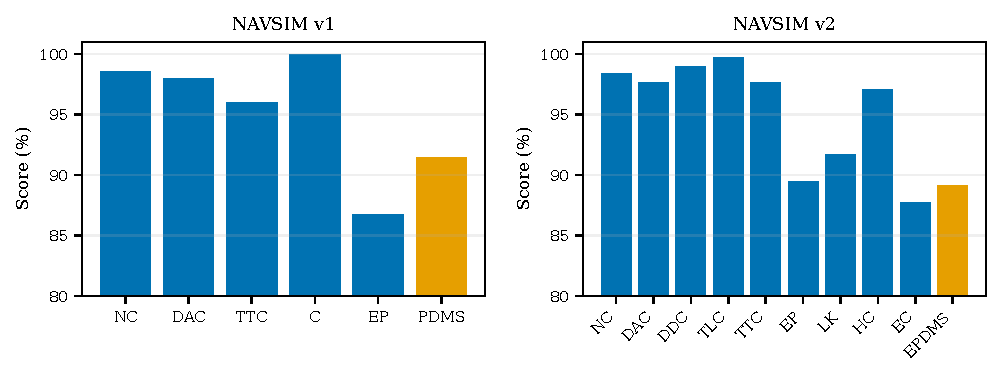
\includegraphics[width=0.76\textwidth]{figures/generated/ampt_metric_profiles.pdf}
  \caption{Scene-level reproduced AMPT component profiles on NAVSIM v1 and
  v2.  All metrics are percentages and higher is better; aggregate PDMS/EPDMS
  is shown in orange.  The profiles use 12,138 and 12,146 scored scenes,
  respectively, from one inference realization.}
  \label{fig:metric-profiles}
\end{figure*}

\paragraph{Single-trajectory inference.}
For each scene and inference seed, the model receives one observation, runs one
five-step denoising chain, and submits its single final $8\times3$ trajectory.
There is no test-time group sampling, evaluator call, candidate scoring,
reference lookup, model ensemble, or reranking.  The v1 submission provenance
independently records candidate count one, so this is a scene-level reproduced
property rather than only a methodological statement.

\paragraph{Runs and uncertainty.}
The archived v1/v2 headline exports each establish a scene-level mean for one
policy realization; they do not establish across-seed variance.  We therefore
do not attach a fabricated standard deviation to the 0.1--0.3 point increments
in the paper.  For the proposed rerun, each of seeds
20260726/20260727/20260728 produces a
complete scene export.  We first compute the mean for each run and report the
mean $\pm$ standard deviation across the three runs.  Method differences use
10,000 paired bootstrap resamples of shared scenes (resampling seeds and then
scenes within seed when multiple seeds are present), with a fixed analysis seed
of 2027 and a two-sided 95\% interval.  Recovery proportions use Wilson 95\%
intervals.  Scene bootstrap intervals from one model run describe variation
over the evaluated scenes and are explicitly not interpreted as training-seed
stability.

\paragraph{Model selection disclosure.}
The archived final v1 provenance states that \texttt{navtest} participated in
checkpoint selection.  We therefore describe the headline table as a
paper-reported benchmark comparison, not as a clean held-out model-selection
study.  The proposed rerun selects checkpoints only on the training/validation
partition, seals a checkpoint hash before \texttt{navtest}, and evaluates each
sealed hash once per inference seed.  This disclosure does not change a main
paper number; it narrows the fairness claim to what the available provenance
supports.

\subsection{The Fixed 658-Scene Recovery Protocol}
\label{sec:hard658-protocol}

The hard population is fixed before comparing optimization methods.  A scene
enters the set when the ReCogDrive IL policy receives PDMS zero in all five
sampling attempts because of collision, drivable-area violation, or both.
The resulting intersection contains 658 scene IDs.  A method \emph{recovers} a
scene when its single submitted trajectory has PDMS strictly greater than
zero under the same evaluator; the threshold is not retuned per method.

For consistency with the main paper, every supplementary hard-set analysis
uses the same archived scalar-GRPO versus historical Core-Pareto recovery pair that produced
367 and 440 positive-score scenes.  It does not substitute a later
full-benchmark checkpoint.  On the 658 fixed scenes, scalar GRPO has 367
positive and 291 zero-score outcomes, whereas the manuscript recovery
checkpoint has 440 positive and 218 zero-score outcomes.  Their paired
transition counts are 347 retained successes, 20 new failures, 93 repaired
failures, and 198 persistent failures.  Hence the net recovery is
$93-20=73$ scenes, exactly the change $440-367$, rather than a gain obtained by
hiding newly failed scenes.  The corresponding recovery rates are 55.8\%
(Wilson 95\% CI 52.0--59.5; $n=658$) and 66.9\% (63.2--70.4; $n=658$).  A
10,000-sample paired scene bootstrap gives an absolute difference of 11.1
percentage points with a 95\% interval of 8.1--14.3 points.
These intervals describe one archived checkpoint pair; no training-seed
identifier was retained for this hard-set export.

The fixed-set construction contains 480 DAC-only, 165 collision-only, and 13
joint collision-and-DAC cases according to the archived cause manifest.  The
same IDs and failure labels are used in all hard-set transition and case-table
analyses.  In particular, ``440 recovered'' means 440 positive outcomes on the
fixed original population; the transition table is required whenever the
claim is interpreted as a policy-to-policy improvement.

\subsection{Baseline and Controlled-Comparison Protocol}
\label{sec:baseline-protocol}

\begin{table*}[t]
\centering
\small
\caption{Fair-comparison protocol for main-paper baselines. All methods use one inference candidate and no test-time scorer in the paper table; unreported backbone/sensor/data details are not inferred. Result identity distinguishes reported from reproduced.}
\label{tab:baseline_protocol}
\resizebox{\textwidth}{!}{%
\begin{tabular}{lcccccc}
\toprule
method & backbone & sensors & training\_data & inference\_candidates & test\_time\_scorer & result\_identity \\
\midrule
AMPT & InternVL3-2B + ReCogDrive diffusion planner & multi-view in paper; one audited APR command resolves single camera & NAVSIM plus offline candidate/teacher pools & 1 & no & locally reproduced v1/v2 final rows; camera-manifest discrepancy disclosed \\
ReCogDrive & not disclosed in current PDF & not disclosed in current PDF & not disclosed in current PDF & 1 & no & paper reported \\
DiffusionDriveV2 & not disclosed in current PDF & not disclosed in current PDF & not disclosed in current PDF & 1 & no & paper reported \\
Drive-JEPA & not disclosed in current PDF & not disclosed in current PDF & not disclosed in current PDF & 1 & no & paper reported \\
\bottomrule
\end{tabular}%
}
\end{table*}


AMPT's v1 and v2 rows are locally reproduced from scene-level outputs.  Other
headline baseline rows are values reported in the main paper and their cited
sources; no local checkpoint, common prediction export, or common seed manifest
was found for them.  They are consequently labeled \emph{reported}, not
\emph{reproduced}.  The table records backbone, sensor interface, training
data, number of inference candidates, and use of a test-time scorer whenever
the cited evidence establishes those fields.  An unavailable field is marked
``not established by the audited source'' rather than filled by analogy with
AMPT.

For the GT/Score/Pareto/PC-MTS comparison, the paper reports a shared
initialization, diffusion SFT loss, optimizer, epoch budget, scalar-GRPO
configuration, and evaluation protocol.  The controlled reproduction
additionally seals the candidate-source manifest, fixes the proposed non-GT
sampling probability, matches the accepted candidate count, draws one target
per scene-update, and uses the same three proposed training seeds.  For Scalar GRPO versus FF-PGRPO, all rollout
chains are generated from the same initialization and sampled with the same
seed before the credit function is changed.  For No APR versus Full APR, total
optimizer steps are matched by continuing the no-APR policy with retention
targets.  These are proposed control procedures until their launch manifests
and outputs exist; the main-paper point estimates remain labeled
paper-reported.

\subsection{Reproduction and Integrity Checks}
\label{sec:reproduction-checks}

The canonical dataset stores normalized scores, benchmark and split, method,
stage, variant, round, scene ID, seed when recorded, feasibility/failure
transitions, teacher status, and its source-file/key provenance.  Validation
checks expected scene counts, duplicate scene-method records, score ranges,
the benchmark aggregate formulas, paired scene sets, and failure-state logic.
Final tables and figures are generated from that dataset; a validation failure
stops manuscript generation.  The build manifest records the command, analysis
seed, package versions, Git revision, and SHA-256 hashes of inputs and outputs.
All raw result directories are read-only, and all derived files remain under
the supplementary directory.

\section{PC-MTS Analyses: Supervision--Optimization Alignment}
\label{sec:pcmts-analysis}

This section is needed because the quality of a supervision target and its
value for subsequent policy optimization are different quantities.  PC-MTS is
designed for the latter: it keeps a target only when its score, component-wise
trade-off, local feasibility, and proximity to the frozen learner's rollout
support are jointly acceptable.  We first examine the observed
imitation-to-optimization reversal, and then specify the controls required to
separate policy compatibility from candidate count and training budget.

\subsection{The observed supervision--optimization reversal}
\label{sec:pcmts-mismatch}

Table~\ref{tab:supervision_mismatch} restates the reported comparison from the
main paper and makes the change induced by the common scalar-GRPO stage
explicit.  Score and Pareto selection produce the two strongest imitation
checkpoints (87.2 and 87.5 PDMS), yet both deteriorate under the subsequent
optimizer.  In contrast, PC-MTS deliberately gives up 0.3--0.6 imitation
points relative to those selectors and improves by 4.2 points after the same
optimization stage.  GT supervision also improves, but finishes 0.8 points
below PC-MTS.  Thus, ranking target sets by imitation PDMS would select Pareto,
whereas ranking them by optimized PDMS selects PC-MTS.  This reversal is the
direct evidence for the mismatch claimed in the paper.

\begin{table}[t]
\centering
\small
\caption{Supervision--optimization comparison on NAVSIM v1 under single-trajectory inference. All four rows are one paper-reported run; higher PDMS and GRPO change are better, and no variance is implied.}
\label{tab:supervision_mismatch}
\resizebox{\linewidth}{!}{%
\begin{tabular}{lccccc}
\toprule
method & il\_pdms & post\_scalar\_grpo\_pdms & grpo\_change\_points & evidence & runs \\
\midrule
GT & 86.4 & 90.3 & 3.9 & paper reported & 1 reported \\
Score & 87.2 & 85.8 & -1.4 & paper reported & 1 reported \\
Pareto & 87.5 & 86.7 & -0.8 & paper reported & 1 reported \\
PC-MTS & 86.9 & 91.1 & 4.2 & paper reported & 1 reported \\
\bottomrule
\end{tabular}%
}
\end{table}


\begin{figure}[t]
  \centering
  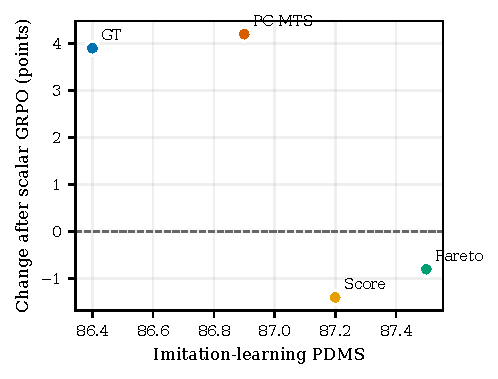
\includegraphics[width=\linewidth]{figures/generated/supervision_mismatch.pdf}
  \caption{Paper-reported imitation PDMS versus the change after the common
  scalar-GRPO stage on NAVSIM v1.  A high imitation score alone does not
  predict optimization value: Score and Pareto regress, whereas PC-MTS gains
  4.2 points.  Each marker is one reported point estimate; the paper does not
  state run/seed aggregation and no synthetic error bars are shown.}
  \label{fig:supervision-mismatch}
\end{figure}

The comparison should be interpreted at the level supported by the evidence.
It demonstrates that a higher-scoring imitation checkpoint need not be a
better starting distribution for GRPO, and that the PC-MTS set is compatible
with a large positive update in this run.  The archived paper table does not
contain scene-level outputs, acceptance counts, or multiple seeds for these
four cells.  Consequently, it does not by itself establish that the reversal
is invariant to seed, nor does it isolate candidate count from the four
filtering decisions.  We therefore do not attach synthetic error bars or
policy-distance values to these points.

\subsection{Candidate-count-matched reconstruction protocol}
\label{sec:pcmts-matched-protocol}

The released reproduction configuration turns the missing causal controls
into a predeclared, low-ambiguity experiment.  All four variants start from the
same GT-only checkpoint, use the same candidate sources, contribute exactly
one target per scene and update, train imitation learning for 200 epochs, and
then run scalar GRPO with 16 rollouts per scene for 10 epochs.  Within each
navigation-command/source stratum, accepted candidates are deterministically
subsampled to the smallest retained count across variants.  The non-GT
sampling probability is held fixed, so a method cannot receive more gradient
updates merely because it retains more candidates.  Empty strata fall back to
the logged trajectory.  In addition to final PDMS, a 300-update diagnostic
records the early GRPO gain before long-horizon training effects can dominate.

For a fully specified reconstruction when the original resolved PC-MTS
manifest is unavailable, the release marks the following as \emph{proposed
reproduction settings}, not measured settings of the reported run: a rollout
bank of 16, $K=3$ neighbors, a command-conditional 0.95 calibration quantile,
and eight temporally correlated local perturbations.  The rollout bank and
calibration queries are disjoint by construction.  Three predeclared training
seeds (20260726, 20260727, and 20260728) are used for the reconstruction, while
bootstrap seed 2027 is reserved for analysis and is never treated as an additional
training run.  These choices fill the executable configuration without
retroactively attributing unrecorded hyperparameters to the main-paper result.

For each run, the pipeline records retained candidates, acceptance rate,
candidate-source composition, feasible rollout rate, feasible high-quality
rate, all-infeasible-group rate, zero-score rate, the 10th percentile,
CVaR-10, 300-update gain, and final scalar-GRPO PDMS.  Method differences are
computed on identical scenes with a 10,000-resample paired bootstrap; means
and standard deviations are reported across the three training seeds.

\subsection{Filter attribution and sensitivity}
\label{sec:pcmts-components}

The component experiment is cumulative: (i) aggregate Score only, (ii) Score
plus the component-wise Pareto gate, (iii) the preceding gates plus calibrated
policy compatibility, and (iv) the full selector with local-feasibility
testing.  Counts are matched after each gate, rather than relaxing a stricter
gate to reach a target count.  This distinction matters: a matched count must
not reintroduce candidates that failed the mechanism being tested.  The
decisive diagnostic is not imitation PDMS alone, but whether adding a gate
raises feasible rollout density and converts the fixed-budget GRPO change from
negative to positive.

The companion sensitivity protocol varies one factor at a time: rollout-bank
size in $\{8,16,32\}$, $K$ in $\{1,3,5\}$, calibration quantile in
$\{0.90,0.95,0.975\}$, and perturbation count in $\{4,8,16\}$.  Compatibility
alternatives are compared at the same acceptance rate: candidate-to-GT
ADE/FDE, distance to the deterministic policy output, minimum rollout-bank
distance, average $K$-nearest distance, and command-calibrated $K$-nearest
distance.  These are evidence-bounded planned analyses: the release contains
their configurations and logging schema, but no unexecuted outcome is used to
support the paper's reported 91.1 PDMS.

Taken together, the existing reversal and the matched protocol close two
different parts of the argument.  The former establishes that isolated target
quality can disagree with downstream optimization value; the latter defines
the experiment needed to attribute that disagreement specifically to policy
compatibility rather than supervision quantity.

\section{FF-PGRPO Analyses: Feasibility Before Positive Credit}
\label{sec:ffpgrpo-analysis}

Aggregate reward can hide an unsafe trade: progress or comfort may increase
enough to give positive standardized advantage even when collision avoidance,
drivable-area compliance, or a protected reference metric regresses.  The
purpose of FF-PGRPO is therefore not merely to reshape the scalar score, but to
change which rollouts are eligible for positive credit.

\subsection{What the stage ablation establishes}
\label{sec:ffpgrpo-stage-ablation}

On NAVSIM v1, the no-stage baseline in the main ablation has 86.5 PDMS, 98.1
NC, 94.7 DAC, 94.2 TTC, and 80.9 EP.  Applying FF-PGRPO without PC-MTS reaches
91.0 PDMS, with 98.4 NC, 98.0 DAC, 95.8 TTC, and 85.93 EP.  With PC-MTS as the
initialization, FF-PGRPO reaches 91.1 PDMS, 98.5 NC, 98.0 DAC, 96.0 TTC, and
86.0 EP before APR.  The improvement is therefore not produced by sacrificing
the displayed hard-safety components for progress: DAC improves by 3.3 points
and TTC by 1.6 points in the FF-PGRPO-only row, while EP increases by 5.03
points.  These are paper-reported point estimates whose run/seed aggregation
is not stated, so the small 0.1-point
difference between the two FF-PGRPO rows is not presented as a stable gain.

\begin{table*}[t]
\centering
\small
\caption{Stage-wise NAVSIM v1 ablation under single-trajectory inference. Higher is better. Rows are one paper-reported run; only the final AMPT row is independently reproduced from 12,138 scene scores.}
\label{tab:stage_ablation}
\resizebox{\textwidth}{!}{%
\begin{tabular}{lcccccccccccc}
\toprule
configuration & pcmts & scalar\_grpo & ff\_pgrpo & apr & NC & DAC & TTC & C & EP & PDMS & evidence & runs \\
\midrule
GT-only & no & no & no & no & 98.1 & 94.7 & 94.2 & 100.0 & 80.9 & 86.5 & paper reported & 1 reported \\
PC-MTS & yes & no & no & no & 98.2 & 95.2 & 94.5 & 100.0 & 81.3 & 86.9 & paper reported & 1 reported \\
Scalar optimization & no & yes & no & no & 98.4 & 98.0 & 95.8 & 100.0 & 85.93 & 91.0 & paper reported & 1 reported \\
PC-MTS + FF-PGRPO & yes & no & yes & no & 98.5 & 98.0 & 96.0 & 100.0 & 86.0 & 91.1 & paper reported & 1 reported \\
Full AMPT & yes & no & yes & yes & 98.5 & 98.0 & 96.0 & 100.0 & 86.7 & 91.4 & paper reported / final row scene-reproduced & 1 reported + 12138 scenes final \\
\bottomrule
\end{tabular}%
}
\end{table*}


This result is consistent with the proposed ordering---recover feasibility,
then optimize continuous quality---but an aggregate stage ablation cannot
directly reveal the sign of individual rollout credits.  The fixed hard-scene
transition in Section~\ref{sec:hard658} provides scene-level evidence, and the
instrumentation below defines the rollout-level test.

\subsection{Credit diagnostics}
\label{sec:ffpgrpo-credit-diagnostics}

For rollout $i$, let $A_i>0$ denote positive assigned advantage and let
$V_i=1$ denote a violation of any hard-feasibility, protected-reference, or
admissible-Pareto condition.  We report
\begin{equation}
  \mathrm{PCVR} =
  \frac{\sum_i \mathbb{1}[A_i>0]V_i}
       {\sum_i \mathbb{1}[A_i>0]},
  \label{eq:positive-credit-violation}
\end{equation}
and separately count reference-regressing and Pareto-dominated positive
credits.  A denominator of zero is reported as ``no positive credits,'' not as
zero violation.  FF-PGRPO's implementation makes a violating rollout
ineligible for positive credit and exposes assertions for this contract.  The
archived training run, however, does not contain the per-rollout trace needed
to quote an observed PCVR; we do not convert a code invariant into a fabricated
measured rate.

The stepwise mechanism ablation adds: (i) the hard feasibility gate, (ii) the
coherent-reference guard, (iii) the Pareto positive-credit gate, and (iv) the
all-infeasible recovery rule.  Every variant logs group state
(all-feasible/mixed/all-infeasible), feasibility rate, positive and negative
advantage means, PCVR, reference-regressing positive-credit rate,
dominated-positive-credit rate, zero-to-feasible repair, positive-to-zero
regression, and updates until the first feasible rollout.  The coherent
reference is always one executable trajectory.  The historical
component-wise envelope remains only as an ablation because combining the best
value of each metric from different trajectories may describe no realizable
plan and can make every sampled rollout appear to regress.

The low-cost diagnostic run uses the paper's group size of 16 and stops at 300
updates; the final run uses the reported 10 epochs.  All variants share the
same sampled rollout tensors when credit is recomputed offline, which makes
the initial credit-assignment comparison independent of policy drift.  New
training is required only for the subsequent learning curves and remains
disabled unless explicitly enabled.

\subsection{Hard-scene evidence for feasibility-first recovery}
\label{sec:ffpgrpo-hard-evidence}

The manuscript recovery checkpoint is evaluated on the same 658-scene set as
scalar GRPO.  Scalar GRPO produces a positive score in 367 scenes (55.8\%,
95\% Wilson CI 52.0--59.5\%), whereas the AMPT recovery checkpoint is positive
in 440 scenes (66.9\%, CI 63.2--70.4\%).  The comparison uses a single
trajectory per scene and neither method uses test-time sampling, scoring, or
reranking.  Crucially, the paired transition is not merely a difference of
gross counts: 93 scalar-GRPO zeros become positive, 20 scalar-GRPO positives
become zero, 347 successes are retained, and 198 failures persist.  Net
recovery is therefore $93-20=73$ scenes, or 11.1 percentage points.  A
10,000-resample scene-paired bootstrap (analysis seed 2027) gives a 95\% CI of
8.1--14.3 percentage points for this paired change.  This interval quantifies
scene variation for this fixed checkpoint pair; it does not replace missing
multi-seed training uncertainty.

The subset mean PDMS increases from 0.5101 to 0.6145.  The corresponding
component means change from 0.8381 to 0.8815 for NC, 0.7052 to 0.7781 for DAC,
0.7705 to 0.8161 for TTC, and 0.4956 to 0.5932 for EP; comfort increases from
0.9985 to 1.0000, while DDC changes from 0.9567 to 0.9521.  This last decrease
is why protected metrics must be reported next to aggregate recovery rather
than summarized as universal component-wise improvement.  The complete
transition and failure-type decomposition are given in
Section~\ref{sec:hard658}.

The aggregate ablation, paired hard-scene transition, and positive-credit
instrumentation serve complementary roles.  The first shows the overall stage
gain, the second verifies that recovery is net positive rather than purchased
entirely with new failures, and the third is the predeclared test of the
claimed credit-assignment mechanism.

\section{APR Analyses: Dynamic, Policy-Relative Teachers}
\label{sec:apr-analysis}

APR addresses a moving-target problem.  A trajectory that is a useful local
teacher for the current policy can become redundant after refinement, while a
previously distant candidate can enter the policy's compatible neighborhood.
The relevant question is therefore not whether additional optimization steps
help, but whether rebuilding and re-auditing the teacher set provides useful
targets while retaining already safe behavior.

\subsection{Round-wise behavior and protected components}
\label{sec:apr-rounds}

The main paper reports a monotonic sequence of 91.10, 91.21, 91.37, and 91.45
PDMS from Round 0 through Round 3, corresponding to gains of $+0.11$, $+0.16$,
and $+0.08$.  In the stage ablation, adding APR to the PC-MTS+FF-PGRPO policy
raises PDMS from 91.1 to 91.4 and EP from 86.0 to 86.7, while the displayed NC,
DAC, TTC, and comfort values remain 98.5, 98.0, 96.0, and 100, respectively.
This pattern is aligned with APR's design: local teacher updates increase
progress without visible regression in the protected components at the
reported precision.

Each round value is a reported checkpoint summary; its run/seed aggregation is
not stated.  No across-seed
standard deviation is available, and the 0.08--0.16 point increments are not
claimed to be independently significant.  Moreover, the archived experiment
history contains accepted and rejected branches rather than a single complete
three-round hash chain; the four values above are therefore treated as the
paper's round-level summary, not as permission to infer missing intermediate
measurements.

\begin{table}[t]
\centering
\small
\caption{Paper-reported NAVSIM v1 APR progression under single-trajectory inference. Higher is better. Run/seed aggregation is not stated and no training-seed confidence interval is available.}
\label{tab:apr_rounds}
\resizebox{\linewidth}{!}{%
\begin{tabular}{lcccc}
\toprule
round & pdms & gain\_points & evidence & runs \\
\midrule
0 & 91.1 & 0.0 & paper reported & reported point; run/seed aggregation not stated \\
1 & 91.21 & 0.11 & paper reported & reported point; run/seed aggregation not stated \\
2 & 91.37 & 0.16 & paper reported & reported point; run/seed aggregation not stated \\
3 & 91.45 & 0.08 & paper reported / final score scene-reproduced & reported point + 12138 final scenes; run aggregation not stated \\
\bottomrule
\end{tabular}%
}
\end{table}


\begin{figure}[t]
  \centering
  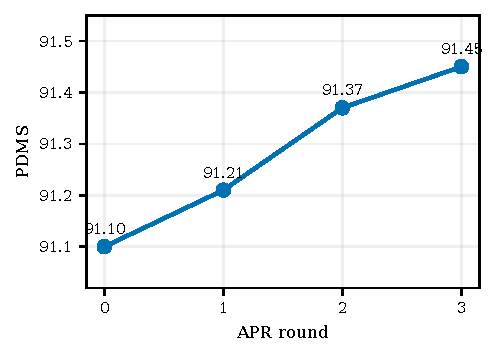
\includegraphics[width=\linewidth]{figures/generated/apr_rounds.pdf}
  \caption{Paper-reported NAVSIM v1 progression across APR rounds.  The final
  point is reproduced at scene level, but the small round increments are from
  one reported sequence and carry no across-seed error bar.}
  \label{fig:apr-rounds}
\end{figure}

\subsection{Teacher audit and post-interpolation evaluation}
\label{sec:apr-teacher-audit}

One traceable APR teacher-construction pass starts from 39,261 strict external
trajectories: 25,402 (64.7\%) from one driving-policy source and 13,859
(35.3\%) from a second source.  After interpolation with coefficient 0.25 and
exact re-evaluation, 28,910 targets remain, an acceptance rate of 73.6\%; the
remaining 10,351 are rejected.  These counts are from one audited navtrain
construction pass and are not presented as the source proportions of every
APR round.  They nevertheless establish an important operational fact:
interpolation is followed by evaluator-based admission, and the check is
non-vacuous---more than one quarter of the pre-audit union does not enter the
distillation set.

\begin{table}[t]
\centering
\small
\caption{Audited APR teacher-pool construction on NAVSIM navtrain. Counts are from one archived teacher audit; the 28,910 accepted teachers follow interpolation and exact re-evaluation. Higher acceptance is not inherently better because guards constrain quality.}
\label{tab:apr_teacher_pool}
\resizebox{\linewidth}{!}{%
\begin{tabular}{lcccc}
\toprule
step & source & count & acceptance\_definition & evidence \\
\midrule
source selection & DriVor & 25402 & source-specific strict candidates & archived APR runbook \\
source selection & DiffusionDriveV2 & 13859 & source-specific strict candidates & archived APR runbook \\
strict union & merged sources & 39261 & feasible and component-protected before interpolation & deterministic sum of audited source counts \\
post-interpolation audit & accepted teachers & 28910 & alpha 0.25 then exact re-evaluation & archived APR runbook \\
\bottomrule
\end{tabular}%
}
\end{table}


Teacher status is defined relative to the current policy.  A candidate is
\emph{accepted} when its evaluated local target is feasible, exceeds the
current single prediction by the required margin, preserves protected
metrics, and stays inside the current rollout neighborhood.  An accepted
teacher becomes \emph{expired} if it fails those tests after the policy is
updated.  A previously rejected candidate is \emph{newly activated} if it
passes after the rollout bank and current prediction are regenerated.  These
definitions prevent lifecycle counts from being conflated with raw pool size.

The interpolation search is descending: larger moves are evaluated first and
the first admissible move is retained.  Every accepted target stores the
teacher, current prediction, interpolation coefficient, post-interpolation
score, protected-metric deltas, compatibility distance, and evaluator hash.
No-interpolation and no-post-evaluation controls remove different safeguards:
the former jumps directly to the teacher, whereas the latter retains a local
trajectory without verifying that interpolation preserved feasibility.

\subsection{Step-matched controls}
\label{sec:apr-controls}

The release defines eight variants from the same Round-0 checkpoint and
matches the total number of optimizer updates: extra training on the existing
mixture, one-shot distillation, repeated use of a fixed teacher set, dynamic
teachers, dynamic teachers without interpolation, without post-interpolation
re-evaluation, without policy retention, and full APR.  The dynamic-teacher
and full-APR variants rebuild predictions, rollout banks, and teacher audits at
the same three round boundaries reported in the paper.  The fixed-teacher
variant repeats the Round-1 set without re-ranking it; the extra-training
control receives the same update count but no new teacher target.  This design
separates four possible explanations: more updates, teacher supervision in
general, teacher-set rebuilding, and the interpolation/retention safeguards.

For every round, the required report contains PDMS and all components,
regressed scenes, new failures, accepted/expired/newly activated teachers,
mean and median verified teacher advantage, interpolation-coefficient
distribution, and scene coverage.  A checkpoint is promoted only if its
single-trajectory aggregate score improves and protected metrics pass the
same non-regression audit; otherwise the previous checkpoint remains the
dynamic anchor.  Training ends after three promoted rounds or when no audited
local target remains.  These controls are configured but not represented as
measured results in this supplement, because running them would require new
training.

Optional task-vector consolidation is kept separate from teacher discovery.
The implementation can mask low-salience coordinates, require directional
agreement, bound each branch norm and the total displacement from the current
anchor, and then evaluate the merged checkpoint.  The best-branch, simple
average, task-arithmetic, and TIES-style controls are required before assigning
an independent gain to merging~\cite{taskarithmetic2023,ties2023}.  In the
absence of a stable, step-matched gain, merging should be read as a conservative
checkpoint-consolidation detail, not as the source of APR's teacher lifecycle.

The present evidence therefore supports two bounded statements: the reported
APR rounds are monotonic and preserve the displayed safety/compliance metrics,
and an audited construction pass materially filters proposed local targets
after re-evaluation.  The step-matched variants above are the necessary test
for the stronger causal claim that dynamic rebuilding, rather than additional
training alone, explains the full increment.

\begin{table}[t]
\centering
\small
\caption{APR fixed-teacher diagnostic on NAVSIM v1. The archived fixed-set continuation decreases from its 91.2766 anchor, whereas the 91.45 endpoint is the paper's compressed dynamic-round report; the rows are diagnostic rather than a step-matched causal ablation.}
\label{tab:apr_fixed_teacher}
\resizebox{\linewidth}{!}{%
\begin{tabular}{lccc}
\toprule
policy\_or\_epoch & pdms & interpretation & evidence \\
\midrule
dynamic-teacher anchor & 91.2766 & accepted dynamic-teacher checkpoint & archived APR runbook \\
fixed-set continuation epoch 0 & 91.2526 & below dynamic-teacher anchor & archived APR runbook \\
fixed-set continuation epoch 1 & 91.2311 & further below dynamic-teacher anchor & archived APR runbook \\
paper APR round 3 & 91.45 & compressed round-level paper report & paper reported \\
\bottomrule
\end{tabular}%
}
\end{table}


\section{Failure Recovery and Qualitative Diagnostics}
\label{sec:failure-qualitative}

Qualitative evidence is most useful when organized by a mechanism and tied to
scene-level metrics.  We therefore analyze the fixed hard set first, then give
traceable examples of recovered, persistent, and newly introduced failures.
All quantitative hard-set results and the mechanism-organized case table use
the same historical checkpoint pair as the main paper's 367-versus-440
recovery claim.  The final full-benchmark visualization is separately labeled
and is not used in the 658-scene recovery analysis.

\subsection{Construction of the fixed 658-scene set}
\label{sec:hard658}

The set contains 658 NAVSIM v1 scenes for which the initial ReCogDrive policy
obtained exactly zero PDMS in all five construction samples because of an
at-fault collision (NC), drivable-area violation (DAC), or both.  The set is
fixed before comparing the scalar-GRPO and AMPT recovery checkpoints.  Under
single-trajectory evaluation, scalar GRPO is positive on 367 and zero on 291
scenes; the AMPT recovery checkpoint is positive on 440 and zero on 218.

The paired $2\times2$ transition is
\begin{equation}
\begin{array}{c|cc|c}
 & \multicolumn{2}{c|}{\text{AMPT recovery checkpoint}} & \\
\text{scalar GRPO} & \text{zero} & \text{positive} & \text{row total} \\
\hline
\text{zero}     & 198 & 93  & 291 \\
\text{positive} & 20  & 347 & 367 \\
\hline
\text{column total} & 218 & 440 & 658
\end{array}.
\label{eq:hard658-transition}
\end{equation}
Hence 93 failures are repaired, 347 successes are retained, 198 failures
persist, and 20 new failures appear.  The net change is $93-20=73$, exactly the
difference between the gross positive counts $440-367$.  This distinction is
important: 440/658 is the gross recovery rate relative to the policy used to
construct the hard set, whereas 93 and 20 describe the paired transition from
scalar GRPO to the AMPT recovery checkpoint.  The resulting 11.1-percentage-
point paired improvement has a scene-bootstrap 95\% CI of 8.1--14.3 points
(10,000 resamples, seed 2027).  It is a net improvement rather than an exchange
of an equal number of old and new failures.

\begin{table}[t]
\centering
\small
\caption{Recovery on the same 658 NAVSIM v1 scenes under one archived comparison. Rates use Wilson 95\% intervals over scenes; this interval does not represent training-seed uncertainty. Higher recovery is better.}
\label{tab:failure_recovery}
\resizebox{\linewidth}{!}{%
\begin{tabular}{lcccccc}
\toprule
Method & Positive & Zero & Recovery rate (\%) & Wilson 95\% CI (\%) & Runs & Scenes \\
\midrule
Scalar GRPO & 367 & 291 & 55.8 & [52.0, 59.5] & 1 archived comparison & 658 \\
AMPT recovery checkpoint & 440 & 218 & 66.9 & [63.2, 70.4] & 1 archived comparison & 658 \\
\bottomrule
\end{tabular}%
}
\end{table}

\begin{table}[t]
\centering
\small
\caption{Paired recovery change on 658 NAVSIM v1 scenes. The 11.1-point gain has a scene-paired bootstrap interval (10,000 resamples, analysis seed 2027); higher net repair is better. One archived model pair is available.}
\label{tab:failure_net_gain}
\resizebox{\linewidth}{!}{%
\begin{tabular}{lcccccc}
\toprule
Absolute gain (pp) & Paired 95\% CI (pp) & Zero-to-positive & Positive-to-zero & Net repair & Scenes & Runs \\
\midrule
11.1 & [8.1, 14.3] & 93 & 20 & 73 & 658 & 1 archived comparison \\
\bottomrule
\end{tabular}%
}
\end{table}


\begin{figure}[t]
  \centering
  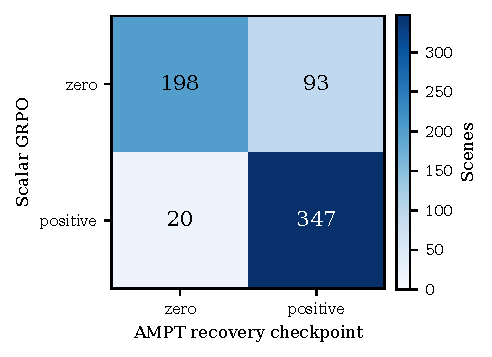
\includegraphics[width=\linewidth]{figures/generated/failure_transition.pdf}
  \caption{Scalar-GRPO to AMPT transition on the fixed 658-scene set.  The
  off-diagonal cells expose both 93 repairs and 20 regressions, rather than
  reporting gross recovery alone.}
  \label{fig:failure-transition}
\end{figure}

The original hard-set taxonomy contains 480 DAC-only scenes, 165 collision-
only scenes, 13 scenes failing both, and no residual ``other'' category.  The
paired repairs/new failures are 59/14 for DAC-only, 32/6 for collision-only,
and 2/0 for the joint category, giving net changes of 45, 26, and 2 scenes.
The gains are therefore not concentrated in only one failure type, although
the small joint category is descriptive rather than statistically decisive.

\begin{table}[t]
\centering
\small
\caption{Failure-type decomposition for the fixed 658 NAVSIM v1 scenes. Repairs and regressions use the scalar-GRPO to AMPT transition; net repairs sum to 73. One archived comparison; higher net repair is better.}
\label{tab:failure_causes}
\resizebox{\linewidth}{!}{%
\begin{tabular}{lcccc}
\toprule
Failure type & Scenes & Repairs & Regressions & Net repair \\
\midrule
DAC-only/all-fail & 480 & 59 & 14 & 45 \\
collision-only/all-fail & 165 & 32 & 6 & 26 \\
collision + DAC & 13 & 2 & 0 & 2 \\
\bottomrule
\end{tabular}%
}
\end{table}


\begin{figure}[t]
  \centering
  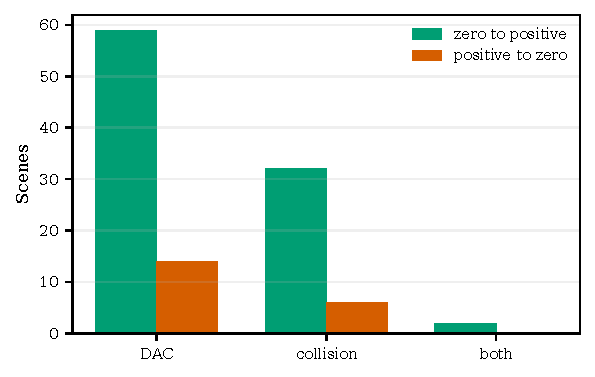
\includegraphics[width=\linewidth]{figures/generated/failure_cause_recovery.pdf}
  \caption{Repairs and regressions by the fixed hard-set cause taxonomy.  The
  net changes are 45 DAC, 26 collision, and 2 joint cases, totaling 73.}
  \label{fig:failure-causes}
\end{figure}

\subsection{Traceable scene cases}
\label{sec:traceable-cases}

Table~\ref{tab:hard658-cases} selects cases by transition type, not by visual
appeal.  Navigation commands come from the corresponding NAVSIM scene
metadata; scores and components come from the fixed paired evaluation.  The
table uses full scene identifiers so every row can be regenerated.  Component
pairs are scalar-GRPO $\rightarrow$ AMPT-recovery values.

\begin{table*}[t]
\centering
\small
\caption{Mechanism-organized examples from the fixed 658-scene set. Scene IDs and PDMS values are reproduced from the archived comparison; commands are joined from audited scene metadata. These selected cases are not an unbiased benchmark sample.}
\label{tab:hard658-cases}
\resizebox{\textwidth}{!}{%
\begin{tabular}{lccccccccc}
\toprule
Scene ID & Command & Outcome & PDMS & NC & DAC & TTC & EP & DDC & Diagnosis \\
\midrule
00fcad6d092c5e8e & left & repaired & 0.000 -> 1.000 & 0.000 -> 1.000 & 1.000 -> 1.000 & 0.000 -> 1.000 & 0.000 -> 1.000 & 1.000 -> 1.000 & Collision/TTC failure repaired without protected regression. \\
03aa8a0576a25b63 & right & repaired & 0.000 -> 0.963 & 1.000 -> 1.000 & 0.000 -> 1.000 & 1.000 -> 1.000 & 0.000 -> 0.912 & 1.000 -> 1.000 & Drivable-area failure repaired while NC and TTC remain feasible. \\
1148c72f141c532d & left & partial repair & 0.000 -> 0.583 & 0.000 -> 1.000 & 0.000 -> 1.000 & 0.000 -> 0.000 & 0.000 -> 1.000 & 1.000 -> 1.000 & Both hard failures repaired; TTC remains the limiting component. \\
00016f8b45c25a1d & left & persistent & 0.000 -> 0.000 & 1.000 -> 1.000 & 0.000 -> 0.000 & 1.000 -> 1.000 & 0.000 -> 0.000 & 0.000 -> 0.000 & DAC/progress failure persists under both audited checkpoints. \\
4b4a268bee4c5ab5 & left & regressed & 1.000 -> 0.000 & 1.000 -> 1.000 & 1.000 -> 0.000 & 1.000 -> 1.000 & 1.000 -> 0.000 & 1.000 -> 1.000 & A DAC regression creates a new zero and motivates retention. \\
\bottomrule
\end{tabular}%
}
\end{table*}


The first two cases are consistent with feasibility-oriented recovery: a hard
component changes from zero to one and positive PDMS returns.  Scene-level
before/after metrics do not identify the temporal order of training updates.
The third shows why ``recovered'' does not mean component-wise perfect.  The
fourth remains a DAC/progress failure under both audited checkpoints; without a
candidate/rollout manifest, the metrics do not identify whether pool coverage,
policy support, or optimization is responsible.  The fifth prevents
survivorship bias in the qualitative analysis and
motivates APR retention; it is one of the 20 positive-to-zero transitions
already charged against net recovery.

\subsection{Mechanism-centered visualization protocol}
\label{sec:qualitative-protocol}

The supplied renderer groups panels by decision rather than by scene
similarity.  A PC-MTS panel overlays an accepted candidate, a rejected distant
candidate, the logged trajectory, and the frozen-policy rollout neighborhood.
An FF-PGRPO mixed-group panel distinguishes unsafe, feasible-but-dominated,
and admissible Pareto-positive rollouts and prints their assigned advantages;
an all-infeasible panel shows the coherent recovery reference.  An APR panel
shows the current prediction, raw teacher, evaluated interpolant, and the
accepted/expired/newly-activated lifecycle state.  Every rendered panel reads
the scene id, command, component scores, and method name from its manifest and
uses a common legend: blue for the current prediction, green for an accepted
or positively credited trajectory, orange for a dominated/expired trajectory,
red for an unsafe trajectory, and black dashed for the coherent reference.

This protocol is also a safeguard against overinterpretation.  A camera/BEV
image is emitted only when the frame, command, all trajectories, and evaluator
record share the same scene identifier.  The metric-only cases in
Table~\ref{tab:hard658-cases} remain quantitative case studies if those visual
assets are unavailable; no unrelated camera frame or hand-drawn trajectory is
substituted merely to complete a panel.

\begin{figure*}[t]
  \centering
  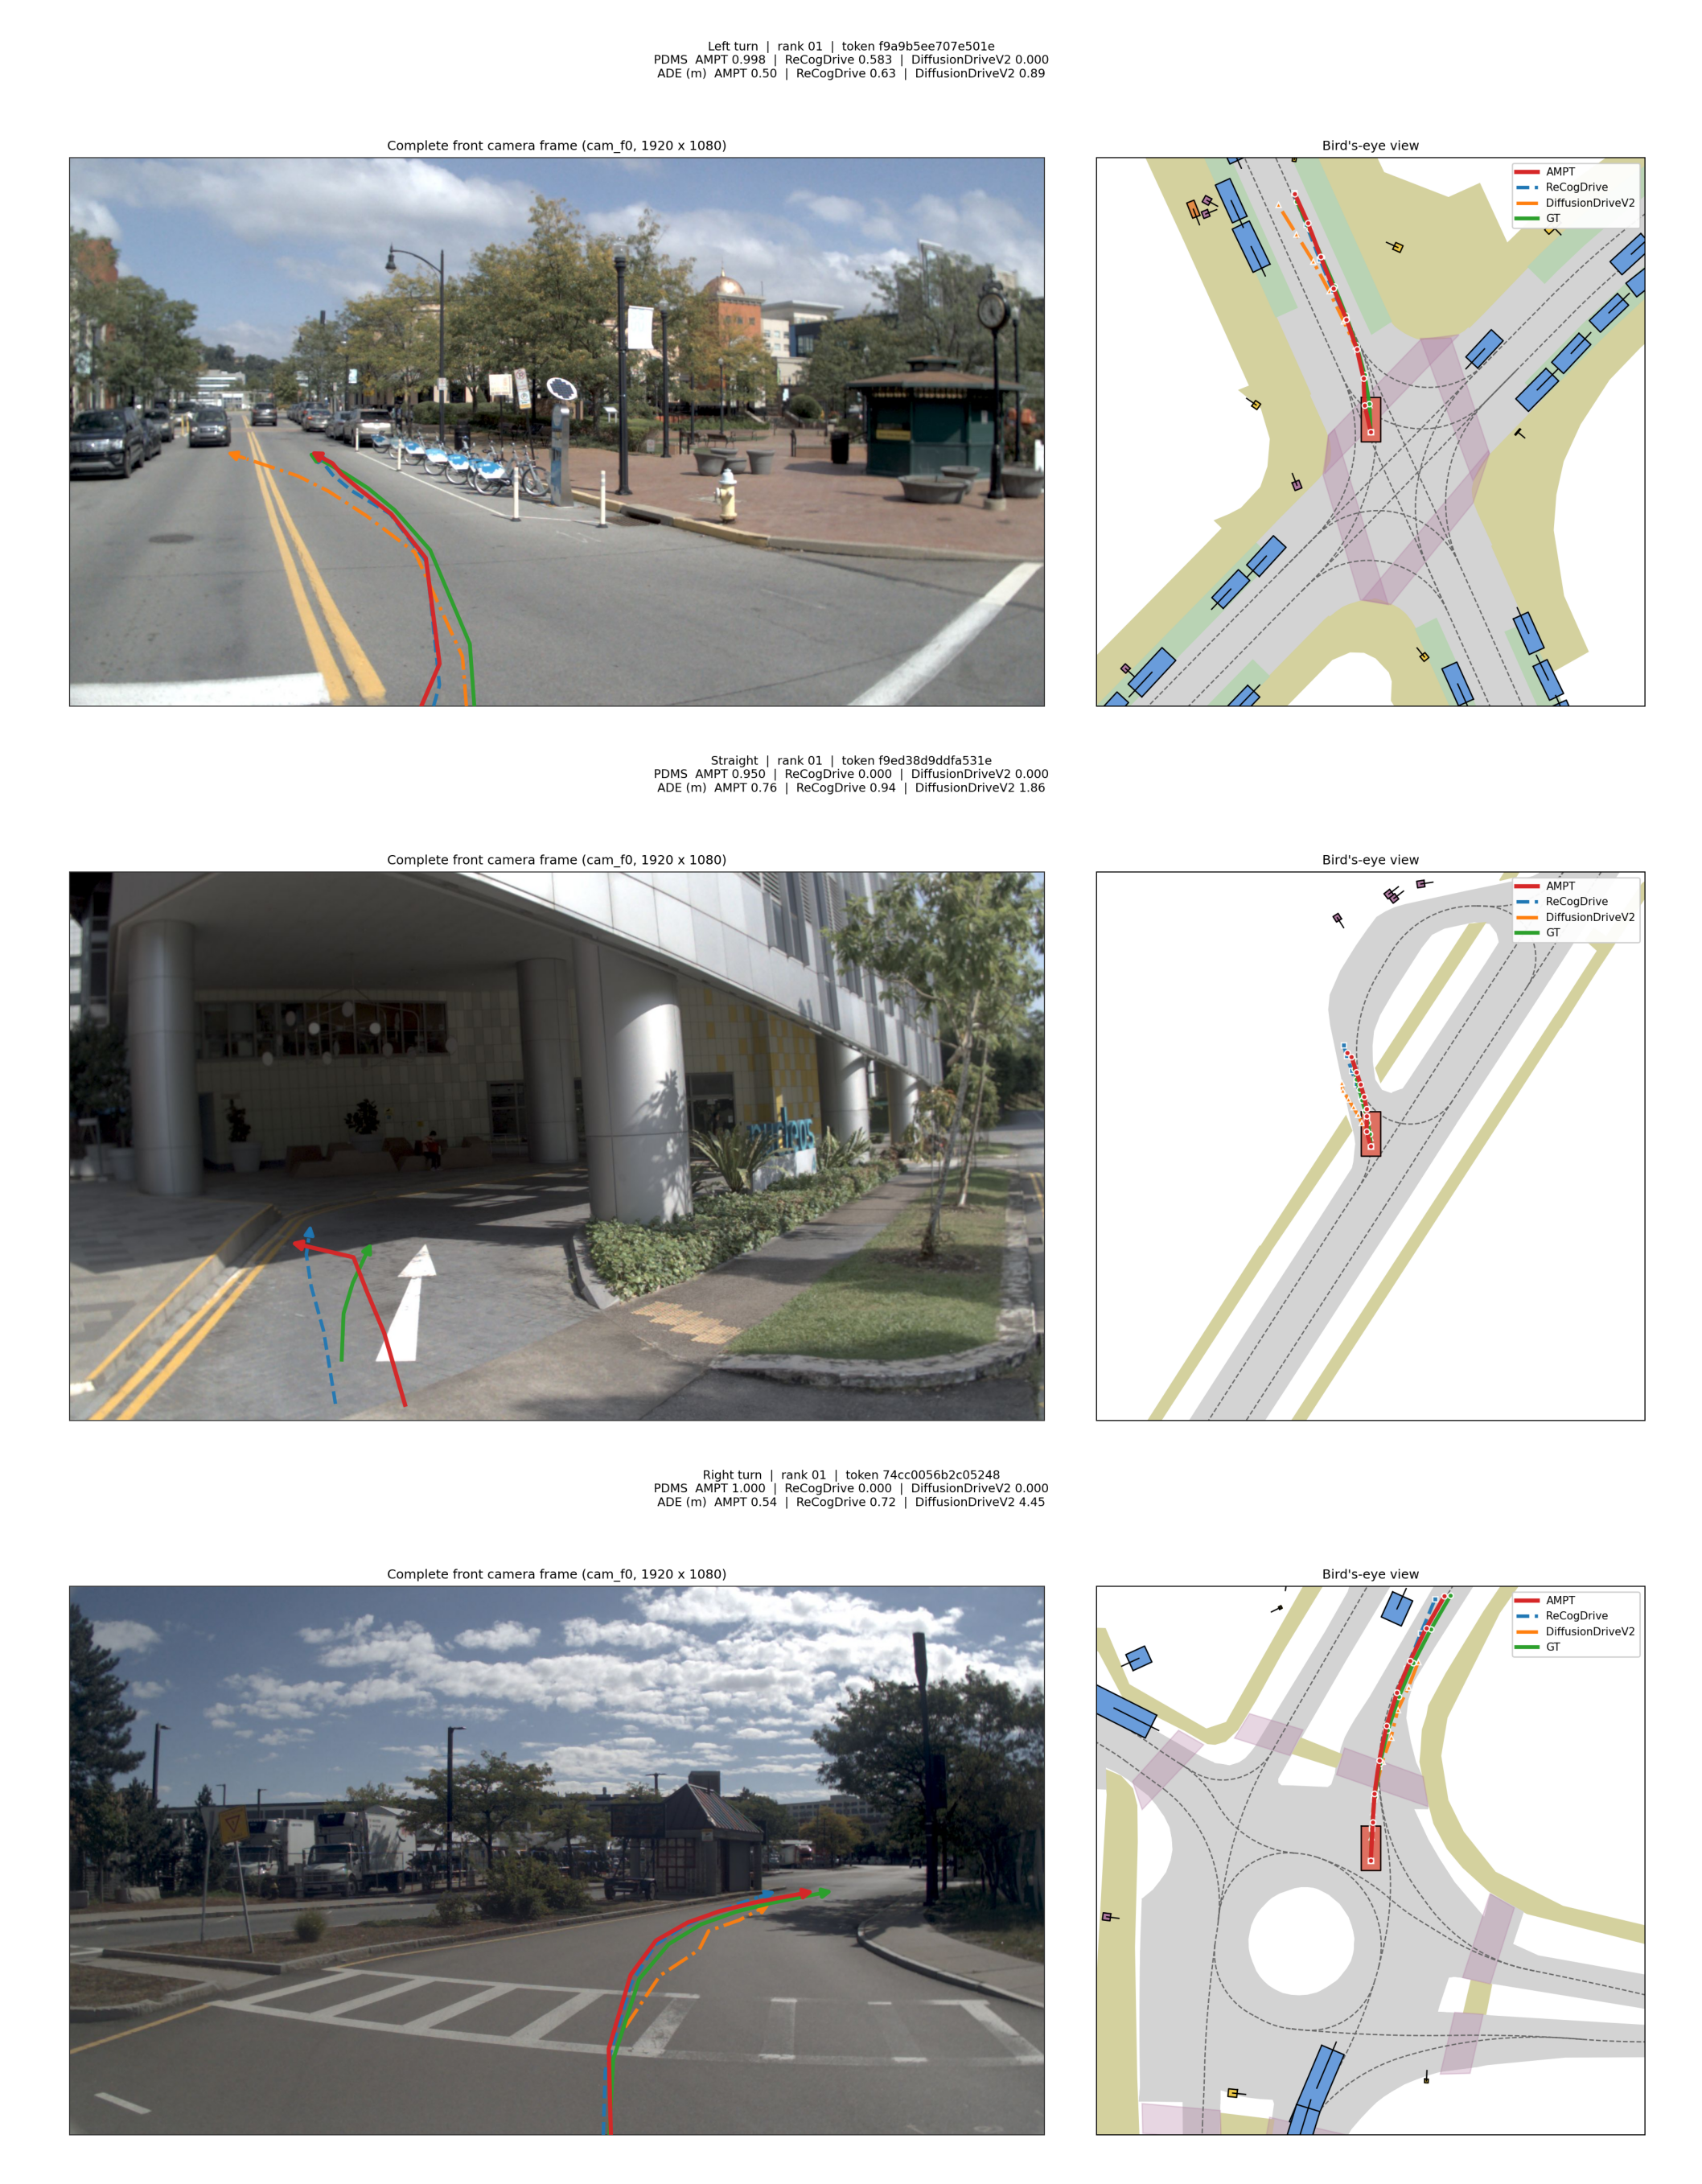
\includegraphics[width=0.92\textwidth]{figures/generated/qualitative_selected_cases.png}
  \caption{Three selected full-benchmark NAVSIM v1 cases (left, straight, and
  right commands) rendered from the separately audited final-AMPT manifest.
  Each row contains the complete front frame, bird's-eye view, scene ID,
  command, color legend, PDMS, and trajectory error.  These examples are not
  members of, and contribute no statistics to, the historical 658-scene
  recovery comparison; they illustrate final-policy behavior only.}
  \label{fig:qualitative-selected}
\end{figure*}

\clearpage

\section{Additional Related Work, Fair Comparison, and Limitations}
\label{sec:related-limitations}

\subsection{Related perspectives}

\textbf{Support-aware policy improvement.}
Conservative offline policy-improvement methods limit updates in regions where
the behavior data provide weak support.  SPIBB constrains uncertain decisions
to the baseline policy~\cite{spibb2019}, while BEAR regularizes a learned policy
toward the behavior distribution~\cite{bear2019}.  PC-MTS shares the support
intuition but applies it before optimization: it filters trajectory-level
supervision using samples from the frozen learner, with command-conditional
calibration and a local feasibility test.  It is not a general monotonic-
improvement guarantee; its role is to avoid moving the imitation policy into a
region where downstream rollout optimization has poor local support.

\textbf{Multi-objective and Pareto optimization.}
Multi-objective reinforcement learning studies policies under vector-valued
returns and alternative preference models~\cite{roijers2013}.  AMPT does not
seek a global set of Pareto-optimal policies.  PC-MTS uses a scene-local Pareto
filter for supervision, and FF-PGRPO uses a hierarchy: hard feasibility and
coherent-reference guards are evaluated before a rollout can receive positive
Pareto credit.  This order is essential when an aggregate score can compensate
for a protected regression.

\textbf{Advantage-weighted behavior learning.}
Advantage-weighted regression turns estimated advantages into weights for
supervised policy updates~\cite{awr2021}.  APR is related at the loss level,
but its weights are attached only after a candidate is compared with the
current single-trajectory prediction, locally interpolated, and re-evaluated.
Teacher admission and policy retention are therefore as important as the
weighting function itself.

\textbf{Model merging.}
Task arithmetic combines model displacements relative to a shared
anchor~\cite{taskarithmetic2023}, and TIES resolves redundancy and sign
conflicts before merging~\cite{ties2023}.  AMPT may use an anchor-constrained
variant to consolidate APR branches, but merging is optional and is separated
from teacher selection.  Passing parameter-space norm and sign checks does not
imply behavioral safety; every merged checkpoint must still undergo the same
single-trajectory evaluator audit.

\subsection{Fair-comparison boundary}
\label{sec:fair-comparison}

AMPT uses one predicted trajectory at inference.  Policy rollout banks,
candidate pools, coherent references, group sampling, specialist policies, and
the offline evaluator are training-only; there is no test-time scorer,
best-of-$N$ selection, or candidate reranking.  This contract is present in the
paper and is independently supported by the v1 submission provenance.

The released v1 scene export contains 12,138 successfully scored scenes from
12,146 predictions; the eight unscored predictions are disclosed rather than
imputed.  The v2 export contains 12,146 successful scene scores.  Its EC
aggregation follows the official evaluator, although a direct EC value is
present for 10,040 rows.  Scene-bootstrap intervals resample these scored
scenes and are explicitly labeled as scene uncertainty; they are not a
substitute for independent training runs.

The baseline rows in the main tables are treated as \emph{reported} unless a
local scene export and matching protocol are available.  AMPT's v1/v2 rows are
reproduced from scene-level outputs, but protocol matching is not established
for every external baseline.  Moreover, the audited v1 provenance records use
of navtest for checkpoint selection.  We therefore avoid a strict held-out
state-of-the-art claim and report protocol fields---backbone, sensors, training
data, inference candidates, and test-time scoring---alongside each comparison.

The 658-scene result uses the recovery checkpoint and checkpoint pair specified
by the main-paper analysis.  It is a fixed-subset diagnostic, not a claim that
every later checkpoint must induce the same transitions.  Reporting the full
$2\times2$ matrix in Eq.~\ref{eq:hard658-transition} makes the gross and net
notions of recovery explicit.

\subsection{Limitations}
\label{sec:limitations}

\textbf{Finite support estimates.}
Compatibility is estimated from a finite rollout bank.  Sparse commands or
multi-modal scenes can make a genuinely useful target appear distant, and the
calibrated neighborhood is only as representative as the frozen policy
samples.  Increasing bank size improves coverage but raises offline inference
and storage cost.

\textbf{Evaluator bias and non-reactive evaluation.}
All three stages use an offline NAVSIM evaluator for filtering, credit, or
teacher validation.  Systematic evaluator errors can therefore be amplified
across stages.  NAVSIM's non-reactive agents also cannot reveal how other road
users would respond to the learned trajectory; feasibility under this scorer
is not a closed-loop safety guarantee.

\textbf{Candidate-pool ceiling.}
APR can select and localize only behaviors represented in its multi-source
pool.  If no source proposes a valid maneuver, rebuilding the pool changes no
target.  The persistent case in Table~\ref{tab:hard658-cases} establishes
persistence under two audited checkpoints, but cannot diagnose this pool
ceiling without a per-scene candidate manifest.

\textbf{Locality can reject long-horizon value.}
The policy-compatibility filter intentionally favors learnable local targets.
It may reject a distant behavior that is initially difficult to imitate but
would be valuable after a longer curriculum.  Policy-dependent teacher-value
and cross-policy selection experiments are therefore important follow-ups.

\textbf{Benchmark-specific hierarchy.}
The ordering of NC/DAC feasibility, DDC/TLC guards, progress floors, and
continuous Pareto objectives reflects NAVSIM metrics.  Transferring AMPT to a
new benchmark requires revalidating the hierarchy and calibration thresholds,
not merely renaming metric fields.

\textbf{No behavioral semantics for parameter merging.}
Task-vector masks, direction agreement, and norm constraints bound parameter
movement but do not provide a semantic or safety guarantee.  If its independent
gain is not stable across seeds and step-matched controls, merging should
remain an implementation detail.

\textbf{Statistical scope.}
The supervision comparison, stage ablation, and APR round table are available
as reported point estimates rather than three-seed aggregates.  Small APR
increments must not be described as stable until the configured multi-seed
controls are run.  The paired 658-scene interval establishes a robust scene-
level net transition for one checkpoint pair, but does not measure training-
seed variation.

These limitations narrow rather than alter the paper's central claim.  The
currently traceable evidence establishes the supervision--optimization
reversal, a large feasibility-oriented stage gain, monotonic reported APR
rounds with preserved displayed safety components, and positive net recovery
on a fixed hard set.  Candidate-count matching, rollout-level credit traces,
step-matched APR controls, and multi-seed reruns are the remaining experiments
needed for stronger causal and stability claims.


\bibliographystyle{plain}
\bibliography{supplementary}
\end{document}
